% Welcome to openmp-examples.tex.
% This is the main LaTex file for the OpenMP Examples document.
%
% The files in this set include:
%
%    openmp-examples.tex              - this file, the main file
%    Makefile                         - makes the document
%    openmp.sty                       - the main style file
%    Title_Page.tex                   - the title page
%    openmplogo.png                   - the logo
%    Forward_Chapt.tex                - unnumbered introductory chapter
%    Chap_*.tex                       - example chapters
%    */sources/*.c, *.f               - C/C++/Fortran example source files
%
% When editing this file:
%
%    1. To change formatting, appearance, or style, please edit openmp.sty.
%
%    2. Custom commands and macros are defined in openmp.sty.
%
%    3. Be kind to other editors -- keep a consistent style by copying-and-pasting to
%       create new content.
%
%    4. We use semantic markup, e.g. (see openmp.sty for a full list):
%         \code{}     % for bold monospace keywords, code, operators, etc.
%         \plc{}      % for italic placeholder names, grammar, etc.
%
%    5. Other recommendations:
%         Use the convenience macros defined in openmp.sty for the minor headers
%         such as Comments, Syntax, etc.
%
%         To keep items together on the same page, prefer the use of 
%         \begin{samepage}.... Avoid \parbox for text blocks as it interrupts line numbering.
%         When possible, avoid \filbreak, \pagebreak, \newpage, \clearpage unless that's
%         what you mean. Use \needspace{} cautiously for troublesome paragraphs.
%
%         Avoid absolute lengths and measures in this file; use relative units when possible.
%         Vertical space can be relative to \baselineskip or ex units. Horizontal space
%         can be relative to \linewidth or em units.
%
%         Prefer \emph{} to italicize terminology, e.g.:
%             This is a \emph{definition}, not a placeholder.
%             This is a \plc{var-name}.
%

% The following says letter size, but the style sheet may change the size
\documentclass[10pt,letterpaper,twoside,makeidx,hidelinks]{scrreprt}

% input a generated file with additional definitions
\input{generated-include}

% Text to appear in the footer on even-numbered pages:
\newcommand{\footerText}{OpenMP Examples Version \VER{} - \VERDATE}

% Unified style sheet for OpenMP documents:
% This is openmp.sty, the preamble and style definitions for the OpenMP specification.
% This is an include file. Please see the main file for more information.
%
% When editing this file:
%
%    1. To change formatting, appearance, or style, please edit openmp.sty.
%
%    2. Custom commands and macros are defined in openmp.sty.
%
%    3. Be kind to other editors -- keep a consistent style by copying-and-pasting to
%       create new content.
%
%    4. We use semantic markup, e.g. (see openmp.sty for a full list):
%         \code{}     % for bold monospace keywords, code, operators, etc.
%         \plc{}      % for italic placeholder names, grammar, etc.
%
%    5. Other recommendations:
%         Use the convenience macros defined in openmp.sty for the minor headers
%         such as Comments, Syntax, etc.
%
%         To keep items together on the same page, prefer the use of 
%         \begin{samepage}.... Avoid \parbox for text blocks as it interrupts line numbering.
%         When possible, avoid \filbreak, \pagebreak, \newpage, \clearpage unless that's
%         what you mean. Use \needspace{} cautiously for troublesome paragraphs.
%
%         Avoid absolute lengths and measures in this file; use relative units when possible.
%         Vertical space can be relative to \baselineskip or ex units. Horizontal space
%         can be relative to \linewidth or em units.
%
%         Prefer \emph{} to italicize terminology, e.g.:
%             This is a \emph{definition}, not a placeholder.
%             This is a \plc{var-name}.
%
% Quick list of the environments, commands and macros supported. Search below for more details.
%
%    \binding                   % makes header of the same name
%    \comments
%    \constraints
%    \crossreferences
%    \descr
%    \effect
%    \format
%    \restrictions
%    \summary
%    \syntax
%    
%    \code{}                    % monospace, bold
%    \plc{}                     % for any kind of placeholder: italic
%    \begin{codepar}            % for blocks of verbatim code: monospace, bold
%    \begin{boxedcode}          % outlined verbatim code for syntax definitions, prototypes, etc.
%    \begin{indentedcodelist}   % used with,e.g., "where clause is one of the following:"
%
%    \specref{}                 % formats the cross-reference "Section X on page Y"
%    
%    \begin{note}               % black horizontal rule for Notes
%    \end{note}
%    
%    \begin{cspecific}          % blue horizontal rule for C-specific text
%    \end{cspecific}
%    
%    \begin{cppspecific}        % blue horizontal rule for C++ -specific text
%    \end{cppspecific}
%    
%    \begin{ccppspecific}       % blue horizontal rule for C/C++ -specific text
%    \end{ccppspecific}
%    
%    \begin{fortranspecific}    % blue horizontal rule for Fortran-specific text
%    \end{fortranspecific}
%    
%    \glossaryterm              % for use in formatting glossary entries
%    \glossarydefstart
%    \glossarydefend
%
%    \compactitem               % single-spaced itemized lists for the Examples doc
%    \cexample                  % C/C++ code example for the Examples doc
%    \fexample                  % Fortran code example for the Examples doc


\usepackage{comment}            % allow use of \begin{comment}
\usepackage{ifpdf,ifthen}       % allow conditional tests in LaTeX definitions
\usepackage{makecell}           % Allows common formatting in cells with \thread & \makecell


%%%%%%%%%%%%%%%%%%%%%%%%%%%%%%%%%%%%%%%%%%%%%%%%%%%%%%%%%%%%%%%%%%%%%%%%%%%%%%%%%%%%%%%%%%%%%%
% Document data
%
\author{}


%%%%%%%%%%%%%%%%%%%%%%%%%%%%%%%%%%%%%%%%%%%%%%%%%%%%%%%%%%%%%%%%%%%%%%%%%%%%%%%%%%%%%%%%%%%%%
% Fonts

\usepackage{amsmath}
\usepackage{amsfonts}
\usepackage{amssymb}
\usepackage{courier}
\usepackage{helvet}
\usepackage[utf8]{inputenc}

% Main body serif font:
\usepackage{tgtermes}
\usepackage[T1]{fontenc}


%%%%%%%%%%%%%%%%%%%%%%%%%%%%%%%%%%%%%%%%%%%%%%%%%%%%%%%%%%%%%%%%%%%%%%%%%%%%%%%%%%%%%%%%%%%%%
% Graphic elements

\usepackage{graphicx}
\usepackage{framed}    % for making boxes with \begin{framed}
\usepackage{tikz}      % for flow charts, diagrams, arrows
\usepackage{subcaption} % For subfigure
\usepackage{float}      % To fix location of figure: \begin{figure}[H] for no float

%%%%%%%%%%%%%%%%%%%%%%%%%%%%%%%%%%%%%%%%%%%%%%%%%%%%%%%%%%%%%%%%%%%%%%%%%%%%%%%%%%%%%%%%%%%%%
% Page formatting
%
% The PDF and book version need different margin spaces.  The bookbuild
% macro is set by the build system (see Makefile) to determine whether
% we are building the PDF or the print-on-demand book version of the spec.
%
\ifdefined\bookbuild
  % we are building the book version of the spec, so we need to have a bit
  % more margin for the publisher to print
  \usepackage[paperwidth=8in, paperheight=10in,
    top=1.25in, bottom=1.5in, left=1.65in, right=0.85in]{geometry}
  \setlength{\oddsidemargin}{0.875in}
  \setlength{\evensidemargin}{0.385in}
\else
  % we are building the PDF version of the spec, so we can use the default
  % margins
  \usepackage[paperwidth=7.5in, paperheight=9in,
    top=0.75in, bottom=1.0in, left=1.4in, right=0.6in]{geometry}
  \setlength{\oddsidemargin}{0.45in}
  \setlength{\evensidemargin}{0.185in}
\fi
\usepackage{changepage}   % allows left/right-page margin readjustments

\raggedbottom


%%%%%%%%%%%%%%%%%%%%%%%%%%%%%%%%%%%%%%%%%%%%%%%%%%%%%%%%%%%%%%%%%%%%%%%%%%%%%%%%%%%%%%%%%%%%%
% Paragraph formatting

\usepackage{setspace}     % allows use of \singlespacing, \onehalfspacing
\usepackage{needspace}    % allows use of \needspace to keep lines together
\usepackage{parskip}      % removes paragraph indenting

\raggedright
\usepackage[raggedrightboxes]{ragged2e}  % is this needed?

\lefthyphenmin=60         % only hyphenate if the left part is >= this many chars
\righthyphenmin=60        % only hyphenate if the right part is >= this many chars


%%%%%%%%%%%%%%%%%%%%%%%%%%%%%%%%%%%%%%%%%%%%%%%%%%%%%%%%%%%%%%%%%%%%%%%%%%%%%%%%%%%%%%%%%%%%%%
% Bulleted (itemized) lists
%    Align bullets with section header
%    Align text left
%    Small bullets
%    \compactitem for single-spaced lists (used in the Examples doc)

\usepackage{enumitem}     % for setting margins on lists
\setlist{leftmargin=*}    % don't indent bullet items
\renewcommand{\labelitemi}{{\normalsize$\bullet$}} % bullet size

% There is a \compactitem defined in package parlist (and perhaps others), however,
% we'll define our own version of compactitem in terms of package enumitem that
% we already use:
\newenvironment{compactitem}
{\begin{itemize}[itemsep=-1.2ex]}
{\end{itemize}}


%%%%%%%%%%%%%%%%%%%%%%%%%%%%%%%%%%%%%%%%%%%%%%%%%%%%%%%%%%%%%%%%%%%%%%%%%%%%%%%%%%%%%%%%%%%%%%
% Tables

% This allows tables to flow across page breaks, headers on each new page, etc.
\usepackage{supertabular}
\usepackage{caption}


%%%%%%%%%%%%%%%%%%%%%%%%%%%%%%%%%%%%%%%%%%%%%%%%%%%%%%%%%%%%%%%%%%%%%%%%%%%%%%%%%%%%%%%%%%%%%
% Line numbering

\usepackage[pagewise]{lineno}       % for line numbers on left side of the page
\pagewiselinenumbers
\setlength\linenumbersep{6em}
\renewcommand\linenumberfont{\normalfont\small\sffamily}
\nolinenumbers            % start with line numbers off


%%%%%%%%%%%%%%%%%%%%%%%%%%%%%%%%%%%%%%%%%%%%%%%%%%%%%%%%%%%%%%%%%%%%%%%%%%%%%%%%%%%%%%%%%%%%%
% Footers

\usepackage{fancyhdr}     % makes right/left footers
\pagestyle{fancy}
\fancyhead{} % clear all header fields
\cfoot{}
\renewcommand{\headrulewidth}{0pt}

% Left side on even pages:
% This requires that \footerText be defined in the main document:
\fancyfoot[LE]{\bfseries \thepage \mdseries \hspace{2em} \footerText}
\fancyhfoffset[E]{4em}

% Right side on odd pages:
\fancyfoot[RO]{\mdseries  \leftmark \hspace{2em} \bfseries \thepage}


%%%%%%%%%%%%%%%%%%%%%%%%%%%%%%%%%%%%%%%%%%%%%%%%%%%%%%%%%%%%%%%%%%%%%%%%%%%%%%%%%%%%%%%%%%%%%
% Section header format - we use four levels: \chapter \section \subsection \subsubsection.

\usepackage{titlesec}     % format headers with \titleformat{}
\usepackage{tocloft}

% Format and spacing for chapter, section, subsection, and subsubsection headers:

\setcounter{secnumdepth}{4}          % show numbers down to subsubsection level

\titleformat{\chapter}[hang]%
{\normalfont\sffamily\upshape\Huge\bfseries\fontsize{20}{20}\selectfont}%
{\thechapter}{0.5em}{}
\titlespacing{\chapter}{0ex}{0em plus 1em minus 1em}{2em plus 1em minus 0em}[10em]

\titleformat{\section}[hang]{\huge\bfseries\sffamily\fontsize{16}{16}\selectfont}{\thesection}{0.5em}{}
\titlespacing{\section}{0em}{3em plus 1em minus 1em}{1em plus 0.5em minus 0em}[10em]

\titleformat{\subsection}[hang]{\LARGE\bfseries\sffamily\fontsize{14}{14}\selectfont}{\thesubsection}{0.5em}{}
\titlespacing{\subsection}{0em}{3em plus 1em minus 1em}{0.75em plus 0.5em minus 0em}[10em]

\titleformat{\subsubsection}[hang]{\needspace{1\baselineskip}%
\Large\bfseries\sffamily\fontsize{12}{12}\selectfont}{\thesubsubsection}{0.5em}{}
\titlespacing{\subsubsection}{0em}{3em plus 1em minus 1em}{0.5em plus 0.5em minus 0em}[10em]

\setlength{\cftbeforetoctitleskip}{1.0ex}
\setlength{\cftaftertoctitleskip}{3.0ex}
\setlength{\cftbeforeloftitleskip}{1.0ex}
\setlength{\cftafterloftitleskip}{3.0ex}
\setlength{\cftbeforelottitleskip}{1.0ex}
\setlength{\cftafterlottitleskip}{3.0ex}
\renewcommand{\cftchapaftersnum}{}
\makeatletter
\renewcommand{\l@section}{\@dottedtocline{1}{1.5em}{2.6em}}
\renewcommand{\l@subsection}{\@dottedtocline{2}{4.1em}{3.4em}}
\makeatother

%%%%%%%%%%%%%%%%%%%%%%%%%%%%%%%%%%%%%%%%%%%%%%%%%%%%%%%%%%%%%%%%%%%%%%%%%%%%%%%%%%%%%%%%%%%%%%
% Macros for minor headers: Summary, Syntax, Description, etc.
% These headers are defined in terms of \paragraph

\titleformat{\paragraph}[block]{\large\bfseries\sffamily\fontsize{11}{11}\selectfont}{}{}{}
\titlespacing{\paragraph}{0em}{1.5em plus 0.55em minus 0.5em}{0.0em plus 0.55em minus 0.0em}

% Use one of the convenience macros below, or \littleheader{} for an arbitrary header
\newcommand{\littleheader}[1] {\paragraph*{#1}}

\newcommand{\binding} {\littleheader{Binding}}
\newcommand{\comments} {\littleheader{Comments}}
\newcommand{\constraints} {\littleheader{Constraints on Arguments}}
\newcommand{\crossreferences} {\littleheader{Cross References}}
\newcommand{\descr} {\littleheader{Description}}
\newcommand{\effect} {\littleheader{Effect}}
\newcommand{\format} {\littleheader{Format}}
\newcommand{\restrictions} {\littleheader{Restrictions}}
\newcommand{\summary} {\littleheader{Summary}}
\newcommand{\syntax} {\littleheader{Syntax}}

\usepackage{scrlayer}
\DeclareNewLayer[foreground,textarea,contents={
\phantom{a}
\emph{This page intentionally left blank}
    }
]{intentionally.text}
\DeclareNewPageStyleByLayers{intentionally}{intentionally.text}
\renewcommand{\cleardoublepage}{\cleardoubleoddpageusingstyle{intentionally}}
\newcommand{\chapdirname}{}
\newcommand{\cchapter}[2] {\cleardoublepage\chapter{#1}%
   \renewcommand{\chapdirname}{#2}}
\newcommand{\bchapter}[1] {\chapter*{#1}%
   \addcontentsline{toc}{chapter}{\protect\numberline{}#1}}
%\newcommand{\sinput}[1] {\input{\chapdirname/#1}}


%%%%%%%%%%%%%%%%%%%%%%%%%%%%%%%%%%%%%%%%%%%%%%%%%%%%%%%%%%%%%%%%%%%%%%%%%%%%%%%%%%%%%%%%%%%%%%
% Code and placeholder semantic tagging.
%
% When possible, prefer semantic tags instead of typographic tags. The
% following semantics tags are defined here:
%
%     \code{}     % for bold monospace keywords, code, operators, etc.
%     \plc{}      % for italic placeholder names, grammar, etc.
%
% For function prototypes or other code snippets, you can use \code{} as
% the outer wrapper, and use \plc{{} inside. Example:
%
%     \code{\#pragma omp directive ( \plc{some-placeholder-identifier} :}
%
% To format text in italics for emphasis (rather than text as a placeholder),
% use the generic \emph{} command. Example:
%
%     This sentence \emph{emphasizes some non-placeholder words}.

% Enable \alltt{} for formatting blocks of code:
\usepackage{alltt}
\usepackage{toolbox}         % for \toolboxReplace

% This sets the default \code{} font to tt (monospace) and bold:
\newcommand\code[1]{\texttt{\textbf{#1}}}
\newcommand\scode[1]{\protect\textbf{\protect\texttt{\protect\detokenize{#1}}}}

% This defines the \plc{} placeholder font to be tt normal slanted:
\newcommand\plc[1]{\textrm{\textmd{\itshape{#1}}}}
\newcommand\splc[1]{\protect\textit{\protect\textrm{\protect\detokenize{#1}}}}

% This is an updated set of macros for code style work
% kcode - keywords, vcode - value, bcode - base language,
% pvar - variables, pout - program outputs
\protected\def\DoReplaceU#1{\def\utexttmp{#1}%
   \toolboxReplace{_}{\_}\utexttmp\utexttmp}
\protected\def\myreplacedmt#1#2{\def\stexttmp{#1}%
   \toolboxReplace{_}{\_}\stexttmp%
   \toolboxReplace{ }{\rmfamily{ }\ttfamily#2}\stexttmp%
   {\ttfamily#2\stexttmp}}
\newcommand\kcode[1]{\myreplacedmt{#1}{\bfseries\upshape}}
\newcommand\vcode[1]{\myreplacedmt{#1}{\mdseries\upshape}}
\newcommand\bcode[1]{\kcode{#1}}
\newcommand\ucode[1]{\myreplacedmt{#1}{\mdseries\slshape}}
\newcommand\pvar[1]{\ucode{#1}}
\newcommand\pout[1]{\vcode{#1}}
\newcommand\docref[1]{\textrm{\mdseries\itshape{#1}}}
\newcommand\example[1]{\splc{#1}}

\newcommand\examplesrepo{https://github.com/OpenMP/Examples}
\newcommand\examplestree[2]{\href{\examplesrepo/tree/v#1}{#2}}
\newcommand\examplesref[1]{\examplestree{#1}{#1}}
\newcommand\examplesblob[1]{\href{\examplesrepo/blob/#1}{#1}}

% Environment for a paragraph of literal code, single-spaced, no outline, no indenting:
\usepackage{listings}
\lstnewenvironment{codepar}{%
  }{}
%\newenvironment{codepar}[1]
%{\begin{alltt}\bfseries #1}
%{\end{alltt}}

% For blocks of code inside a box frame:
\lstnewenvironment{boxedcode}{%
  \lstset{framesep=1.2ex,frame=l,framerule=3pt,
          backgroundcolor=\color{white!90!black}}}{}
\lstnewenvironment{boxeducode}{%
  \lstset{framesep=1.2ex,frame=l,framerule=3pt,
          basicstyle=\ttfamily\mdseries\slshape,
          backgroundcolor=\color{white!90!black}}}{}
%\newenvironment{boxedcode}[1]
%{\vspace{0.25em plus 5em minus %0.25em}\begin{framed}\begin{minipage}[t]{\textwidth}\begin{alltt}\bfseries #1}
%{\end{alltt}\end{minipage}\end{framed}\vspace{0.25em plus 5em minus 0.25em}}

% This sets the margins in the framed box:
\setlength{\FrameSep}{0.6em}

% For indented lists of verbatim code at a relaxed line spacing,
% e.g., for use after "where clause is one of the following:"
\usepackage{setspace}
\lstnewenvironment{indentedcodelist}{%
  \lstset{xleftmargin=0.25in}}{}
%\newenvironment{indentedcodelist}{%
%\begin{adjustwidth}{0.25in}{}\vspace{-0.2\baselineskip}\begin{spacing}{1.2}\beg%in{alltt}\bfseries}
%    {\end{alltt}\end{spacing}\vspace{-0.2\baselineskip}\end{adjustwidth}}

\lstdefinestyle{openmp}{
  showstringspaces=false,
  basicstyle=\ttfamily\bfseries,
  linewidth=.99\linewidth,
  xleftmargin=0.01\linewidth,
  columns=fullflexible,
  keepspaces=true,
  escapechar=@,
  belowskip=\smallskipamount,
  aboveskip=\smallskipamount,
  morecomment=[l][\color{red}\sout]{\%DIF\ <},         % deleted empty lines
  morecomment=[l][\color{blue}\uwave]{\%DIF\ >},       % added empty lines
  moredelim=[il][\color{red}\sout]{\%DIF\ <\ },        % deleted lines
  moredelim=[il][\color{blue}\uwave]{\%DIF\ >\ },      % added lines
  moredelim=**[is][\rmfamily\mdseries\itshape]{\\plc\{}{\}},
  moredelim=**[is][\textsubscript]{\\textsubscript\{}{\}},
  moredelim=**[is][]{\\textnormal\{}{\}},
  moredelim=**[is][\rmfamily\mdseries\itshape]{\\textsl\{}{\}},
  moredelim=**[is][\ttfamily\mdseries\slshape]{\\ucode\{}{\}},
  moredelim=**[is][\ttfamily\bfseries\upshape]{\\kcode\{}{\}},
  moredelim=**[is][]{\\code\{}{\}},
  moredelim=**[is][]{\\scode\{}{\}},
  moredelim=*[is][\color{red}\sout]{*!----}{----!*},
  moredelim=*[is][\color{blue}\uwave]{*!++++}{++++!*},
  moredelim=**[is][\mdseries\rmfamily]{\\text\{}{\}},
}
\lstset{style=openmp}


%%%%%%%%%%%%%%%%%%%%%%%%%%%%%%%%%%%%%%%%%%%%%%%%%%%%%%%%%%%%%%%%%%%%%%%%%%%%%%%%%%%%%%%%%%%%%%
% Macros for the black and blue lines and arrows delineating language-specific
% and notes sections. Example:
%
%   \fortranspecificstart
%   This is text that applies to Fortran.
%   \fortranspecificend

% local parameters for use \linewitharrows and \notelinewitharrows:
\newlength{\sbsz}\setlength{\sbsz}{0.05in}  % size of arrows
\newlength{\sblw}\setlength{\sblw}{1.35pt}  % line width (thickness)
\newlength{\sbtw}                           % text width
\newlength{\sblen}                          % total width of horizontal rule
\newlength{\sbht}                           % height of arrows
\newlength{\sbhadj}                         % vertical adjustment for aligning arrows with the line
\newlength{\sbns}\setlength{\sbns}{7\baselineskip}       % arg for \needspace for downward arrows

% \notelinewitharrows is a helper command that makes a black Note marker:
%     arg 1 = 1 or -1 for up or down arrows
%     arg 2 = solid or dashed or loosely dashed, etc.
\newcommand{\notelinewitharrows}[2]{%
    \needspace{0.1\baselineskip}%
    \vbox{\begin{tikzpicture}%
        \setlength{\sblen}{\linewidth}%
        \setlength{\sbht}{#1\sbsz}\setlength{\sbht}{1.4\sbht}%
        \setlength{\sbhadj}{#1\sblw}\setlength{\sbhadj}{0.25\sbhadj}%
        \filldraw (\sblen, 0) -- (\sblen - \sbsz, \sbht) -- (\sblen - 2\sbsz, 0) -- (\sblen, 0);
        \draw[line width=\sblw, #2] (2\sbsz - \sblw, \sbhadj) -- (\sblen - 2\sbsz + \sblw, \sbhadj);
        \filldraw (0, 0) -- (\sbsz, \sbht) -- (0 + 2\sbsz, 0) -- (0, 0);
    \end{tikzpicture}}}

% \linewitharrows is a helper command that makes a blue horizontal line, up or down arrows, and some text:
% arg 1 = 1 or -1 for up or down arrows
% arg 2 = solid or dashed or loosely dashed, etc.
% arg 3 = text
% arg 4 = text width
\newcommand{\linewitharrows}[4]{%
    \needspace{0.1\baselineskip}%
    \vbox to 1\baselineskip {\begin{tikzpicture}%
        \setlength{\sbtw}{#4}%
        \setlength{\sblen}{\linewidth}%
        \setlength{\sbht}{#1\sbsz}\setlength{\sbht}{1.4\sbht}%
        \setlength{\sbhadj}{#1\sblw}\setlength{\sbhadj}{0.25\sbhadj}%
        \filldraw[color=blue!40] (\sblen, 0) -- (\sblen - \sbsz, \sbht) -- (\sblen - 2\sbsz, 0) -- (\sblen, 0);
        \draw[line width=\sblw, color=blue!40, #2] (2\sbsz - \sblw, \sbhadj) -- (0.5\sblen - 0.5\sbtw, \sbhadj);
        \draw[line width=\sblw, color=blue!40, #2] (0.5\sblen + 0.5\sbtw, \sbhadj) -- (\sblen - 2\sbsz + \sblw, \sbhadj);
        \filldraw[color=blue!40] (0, 0) -- (\sbsz, \sbht) -- (0 + 2\sbsz, 0) -- (0, 0);
        \node[color=blue!90] at (0.5\sblen, 0) {\large  \textsf{\textup{#3}}};
    \end{tikzpicture}}}

\newcommand{\VSPb}{\vspace{0.5ex plus 5ex minus 0.25ex}}
\newcommand{\VSPa}{\vspace{0.25ex plus 5ex minus 0.25ex}}

% remove language marker definition if either ccpp or fortran is undefined
\ifthenelse{\boolean{ccpp}\and\boolean{fortran}}{}%
{\renewcommand{\linewitharrows}[4]{\par}}
\newcommand{\langselect}{}
\ifccpp\else\renewcommand{\langselect}{Fortran~}\fi
\iffortran\else\renewcommand{\langselect}{C/C++~}\fi

% C
\ifccpp
\newenvironment{cspecific}[1][0ex]{\vspace{#1}\cspecificstart\vspace{-#1}}{\cspecificend}
\else
\excludecomment{cspecific}
\fi
\newcommand{\cspecificstart}{\needspace{\sbns}\linewitharrows{-1}{solid}{C}{3em}}
\newcommand{\cspecificend}{\linewitharrows{1}{solid}{C}{3em}\bigskip}

% C/C++
\ifccpp
\newenvironment{ccppspecific}[1][0ex]{\vspace{#1}\ccppspecificstart\vspace{-#1}}{\ccppspecificend}
\else
\excludecomment{ccppspecific}
\fi
\newcommand{\ccppspecificstart}{\VSPb\linewitharrows{-1}{solid}{C / C++}{6em}\VSPa}
\newcommand{\ccppspecificend}{\VSPb\linewitharrows{1}{solid}{C / C++}{6em}\VSPa}

% C++
\ifccpp
\newenvironment{cppspecific}[1][0ex]{\vspace{#1}\cppspecificstart\vspace{-#1}}{\cppspecificend}
\else
\excludecomment{cppspecific}
\fi
\newcommand{\cppspecificstart}{\needspace{\sbns}\linewitharrows{-1}{solid}{C++}{6em}}
\newcommand{\cppspecificend}{\linewitharrows{1}{solid}{C++}{6em}\bigskip}

% C90
\newenvironment{cNinetyspecific}{\cNinetyspecificstart}{\cNinetyspecificend}
\newcommand{\cNinetyspecificstart}{\needspace{\sbns}\linewitharrows{-1}{solid}{C90}{4em}}
\newcommand{\cNinetyspecificend}{\linewitharrows{1}{solid}{C90}{4em}\bigskip}

% C99
\newenvironment{cNinetyNinespecific}{\cNinetyNinespecificstart}{\cNinetyNinespecificend}
\newcommand{\cNinetyNinespecificstart}{\needspace{\sbns}\linewitharrows{-1}{solid}{C99}{4em}}
\newcommand{\cNinetyNinespecificend}{\linewitharrows{1}{solid}{C99}{4em}\bigskip}

% Fortran
\iffortran
\newenvironment{fortranspecific}[1][0ex]{\vspace{#1}\fortranspecificstart\vspace{-#1}}{\fortranspecificend}
\else
\excludecomment{fortranspecific}
\fi
\newcommand{\fortranspecificstart}{\VSPb\linewitharrows{-1}{solid}{Fortran}{6em}\VSPa}
\newcommand{\fortranspecificend}{\VSPb\linewitharrows{1}{solid}{Fortran}{6em}\VSPa}

% Note
\newenvironment{note}{\notestart}{\noteend}
\newcommand{\notestart}{\VSPb\notelinewitharrows{-1}{solid}\VSPa}
\newcommand{\noteend}{\VSPb\notelinewitharrows{1}{solid}\VSPa}

% convenience macro for formatting the word "Note:" at the beginning of note blocks:
\newcommand{\noteheader}{{\textrm{\textsf{\textbf\textup\normalsize{{{{Note }}}}}}}}

% blue line floater at top of a page for "Name (cont.)"
\newcommand{\topmarker}[1]{%
  \begin{figure}[t!]
  \linewitharrows{-1}{dashed}{#1 (cont.)}{8em}
  \end{figure}}


%%%%%%%%%%%%%%%%%%%%%%%%%%%%%%%%%%%%%%%%%%%%%%%%%%%%%%%%%%%%%%%%%%%%%%%%%%%%%%%%%%%%%%%%%%%%%%
% Glossary formatting

\newcommand{\glossaryterm}[1]{\needspace{1ex}
\begin{adjustwidth}{-0.75in}{0.0in}
\nolinenumbers\parbox[b][-0.95\baselineskip][t]{1.4in}{\flushright \textbf{#1}}
\end{adjustwidth}\linenumbers}

\newcommand{\glossarydefstart}{
\begin{adjustwidth}{0.79in}{0.0in}}

\newcommand{\glossarydefend}{
\end{adjustwidth}\vspace{-1.5\baselineskip}}


%%%%%%%%%%%%%%%%%%%%%%%%%%%%%%%%%%%%%%%%%%%%%%%%%%%%%%%%%%%%%%%%%%%%%%%%%%%%%%%%%%%%%%%%%%%%%
% Indexing and Table of Contents

\usepackage{makeidx}
\usepackage[nodotinlabels]{titletoc}   % required for its [nodotinlabels] option

% Clickable links in TOC and index:
\usepackage[hyperindex=true,linktocpage=true]{hyperref}
\hypersetup{
  bookmarksnumbered = true,
  bookmarksopen     = false,
  colorlinks  = true, % Colors links instead of red boxes
  urlcolor    = blue, % Color for external links
  linkcolor   = blue  % Color for internal links
}


%%%%%%%%%%%%%%%%%%%%%%%%%%%%%%%%%%%%%%%%%%%%%%%%%%%%%%%%%%%%%%%%%%%%%%%%%%%%%%%%%%%%%%%%%%%%%
% Formats a cross reference label as "Section X on page Y".

\newcommand{\nspecref}[2]{#1~\ref{#2} on page~\pageref{#2}}
\newcommand{\specref}[1]{\nspecref{Section}{#1}}

% For caption for supertabular and figure, by yanyh15
\captionsetup[table]{labelfont={sf,sc,bf},textfont=normalfont,singlelinecheck=off,labelformat=simple,labelsep=colon,aboveskip=00pt,belowskip=10pt}

\captionsetup[figure]{labelfont={sf,sc,bf},textfont=normalfont,singlelinecheck=off,labelformat=simple,labelsep=colon}


%%%%%%%%%%%%%%%%%%%%%%%%%%%%%%%%%%%%%%%%%%%%%%%%%%%%%%%%%%%%%%%%%%%%%%%%%%%%%%%%%%%%%%%%%%%%%
% Code example formatting for the Examples document
% This defines:
%     \cexample       formats blue markers, caption, and code for C examples
%     \cppexample     formats blue markers, caption, and code for C++ examples
%     \fexample       formats blue markers, caption, and code for Fortran (fixed) examples
%     \ffreeexample   formats blue markers, caption, and code for Fortran90 (free) examples

\usepackage{color,fancyvrb}  % for \VerbatimInput
\usepackage{xargs}           % for optional args

\renewcommand\theFancyVerbLine{\normalfont\footnotesize\sffamily S-\arabic{FancyVerbLine}}

\newcommand{\escstr}[1]{\DoReplaceU{#1}}
\newcommandx*\verlabel[2][1=]{(\code{\small{}#1omp\_#2})}

\newcommand{\exampleheader}[6]{%
   \ifthenelse{ \equal{#1}{} }{
      \def\cname{#2}
      \def\ename\cname
   }{
      \def\cname{#1.#2.#3}
% Use following line for old numbering
%      \def\ename{\thechapter.#2.#3}
% Use following for mneumonics
      \def\ename{\escstr{#1}.\escstr{#2}.#3}
   }
   \newcount\cnt
   \cnt=#4
   \ifthenelse{ \equal{#5}{0} }{}{\global\advance\cnt by #5}

   \def\cverno{\ref{ex_vtag:\cname}}
   \ifthenelse{ \equal{\cverno}{pre_3.0} }{\def\cverno{}}{}
   \ifthenelse{ \equal{\cverno}{??} }{\def\cverno{#6}}{}
   \def\stagcnt{\pageref{ex_vtag:\cname}}
   \ifthenelse{ \equal{\cverno}{} }{
      \global\advance\cnt by 1
      \def\vername{\;\;\verlabel[pre\_]{3.0}}
   }{
      \def\myver##1{\toolboxSplitAt{##1}{_}\lefttext\righttext
         \lefttext\toolboxIfElse{\ifx\righttext\undefined}%
         {\global\advance\cnt by 1}{\expandafter{\righttext}}}
      \def\vername{\;\;\verlabel{\myver{\cverno}}}
   }
   \def\fcnt{\the\cnt}
%   \def\fcnt{\stagcnt}
   \noindent
   \underline{\hypertarget{ex:\cname}{\textit{Example \ename}}\vername}
   %\vspace*{-3mm}
   \code{\VerbatimInput[numbers=left,numbersep=5ex,firstnumber=1,firstline=\fcnt,fontsize=\small]%
      {\chapdirname/sources/\cname}} 
}

\newcommandx*\cnexample[4][1=,4=0]{%
   \exampleheader{#2}{#3}{c}{7}{#4}{#1}
}

\newcommandx*\cppnexample[4][1=,4=0]{%
   \exampleheader{#2}{#3}{cpp}{7}{#4}{#1}
}

\newcommandx*\fnexample[4][1=,4=0]{%
   \exampleheader{#2}{#3}{f}{5}{#4}{#1}
}

\newcommandx*\ffreenexample[4][1=,4=0]{%
   \exampleheader{#2}{#3}{f90}{5}{#4}{#1}
}

\newcommandx*\srcnexample[5][1=,5=0]{%
   \exampleheader{#2}{#3}{#4}{0}{#5}{#1}
}

\newcommandx*\cexample[4][1=,4=0]{%
\ifccpp
\needspace{5\baselineskip}\begin{ccppspecific}
\cnexample[#1]{#2}{#3}[#4]
\end{ccppspecific}
\fi
}

\newcommandx*\cppexample[4][1=,4=0]{%
\ifccpp
\needspace{5\baselineskip}\begin{cppspecific}
\cppnexample[#1]{#2}{#3}[#4]
\end{cppspecific}
\fi
}

\newcommandx*\fexample[4][1=,4=0]{%
\iffortran
\needspace{5\baselineskip}
\begin{fortranspecific}
\fnexample[#1]{#2}{#3}[#4]
\end{fortranspecific}
\fi
}

\newcommandx*\ffreeexample[4][1=,4=0]{%
\iffortran
\needspace{5\baselineskip}
\begin{fortranspecific}
\ffreenexample[#1]{#2}{#3}[#4]
\end{fortranspecific}
\fi
}

\newcommandx*\hexentry[4][1=c,3=]{%
  \hyperlink{ex:#2.#1}{\splc{#2.#1}}%
    \ifthenelse{ \equal{#3}{} }{}{,~\hyperlink{ex:#2.#3}{\plc{#3}}}%
    & #4%:~\splc{same name}
}
\newcommandx*\hexmentry[5][1=c,3=]{%
  \hyperlink{ex:#2.#1}{\splc{#2.#1}}%
    \ifthenelse{ \equal{#3}{} }{}{,~\hyperlink{ex:#2.#3}{\plc{#3}}}%
    & #4:~\splc{#5.#1}\ifthenelse{ \equal{#3}{} }{}{,~\plc{#3}}
}


% Set default fonts:
\rmfamily\mdseries\upshape\normalsize


% This is the end of openmp.sty of the OpenMP specification.


\makeindex

\begin{document}
    \pagenumbering{roman}
    %%%%%%%%%%%%%%%%%%%%%%%%%%%%%%%%%%%%%%%%%%%%%%%%%%%%%%%%%%%%%%%%%%%%%%%%%%%%%%%%%%%%%%%%%%%%%%
% Title page

  \begin{titlepage}
    \begin{flushleft}
     \hspace{-6em} \includegraphics[width=0.4\textwidth]{openmp-logo.png}
    \end{flushleft}

    \begin{adjustwidth}{-0.75in}{0in}
    \begin{center}
      \Huge
      \textsf{OpenMP\\Application Programming\\Interface}

      % An optional subtitle can go here:
      \vspace{0.5in}\textsf{Examples}\vspace{-0.7in}
      \normalsize

      \vspace{1.0in}

      \textbf{Version \PVER{} -- \VERDATE}
    \end{center}
    \end{adjustwidth}

    \vspace{2.3in} %was 3.0

Source codes for OpenMP \VER{} Examples are available at
 \href{https://github.com/OpenMP/Examples/tree/v\VER}%
 {github (https://github.com/OpenMP/Examples/tree/v\VER)}.\\

\begin{adjustwidth}{0pt}{1em}\setlength{\parskip}{0.25\baselineskip}%
Copyright \copyright{} 1997-2022 OpenMP Architecture Review Board.\\
Permission to copy without fee all or part of this material is granted,
provided the OpenMP Architecture Review Board copyright notice and
the title of this document appear. Notice is given that copying is by
permission of OpenMP Architecture Review Board.\end{adjustwidth}

  \end{titlepage}

% Blank page

%\cleardoublepage

%For final version, uncomment the line above, comment out the lines below
%This working version enacted the following tickets: 287, 519, 550, 593, 
%674, 688, 689, 
%and a few other editorial changes.
%\vfill



    \chapter*{Foreword}
\label{chap:foreword}

The OpenMP Examples document has been updated with new features
found in the OpenMP \VER\ Specification. The additional examples and updates
are referenced in the Document Revision History of the Appendix on page~\pageref{chap:history}.

Text describing an example with a \VER\ feature specifically states
that the feature support begins in the OpenMP \VER\ Specification.  Also,
an \code{\small omp\_\VER} keyword is included in the  metadata of the source code.
These distinctions are presented to remind readers that a \VER\ compliant 
OpenMP implementation is necessary to use these features in codes.

Examples for most of the \VER\ features are included in this document,
and incremental releases will become available as more feature examples
and updates are submitted and approved by the OpenMP Examples Subcommittee.

Examples are accepted for this document after discussions, revisions and reviews
in the Examples Subcommittee, and two reviews/discussions and two votes
in the OpenMP Language Committee.
Draft examples are often derived from case studies for new features in the language,
and are revised to illustrate the basic application of the features with code comments,
and a text description. We are grateful to the numerous members of the Language Committee 
who took the time to prepare codes and descriptions, and shepherd them through
the acceptance process. We sincerely appreciate the Example Subcommittee members, who 
actively participated and contributed in weekly meetings over the years.

\bigskip
Examples Subcommittee Co-chairs: \smallskip\linebreak
Henry Jin (\textsc{NASA} Ames Research Center) \linebreak
Kent Milfeld (\textsc{TACC}, Texas Advanced Computing Center)



    \thispagestyle{empty}
    \newpage

    \setcounter{page}{1}
    \setcounter{tocdepth}{2}

    \begin{spacing}{1.3}
        \tableofcontents
        \clearpage
        \listoffigures
        \vspace*{5ex}
        \listoftables
    \end{spacing}

    % Uncomment the next line to enable line numbering on the main body text:
    \linenumbers\pagewiselinenumbers

    \cleardoublepage
    \pagenumbering{arabic}

    \setcounter{chapter}{0}  % start chapter numbering here

    % This is the introduction for the OpenMP Examples document.
% This is an included file. See the main file (openmp-examples.tex) for more information.
%
% When editing this file:
%
%    1. To change formatting, appearance, or style, please edit openmp.sty.
%
%    2. Custom commands and macros are defined in openmp.sty.
%
%    3. Be kind to other editors -- keep a consistent style by copying-and-pasting to
%       create new content.
%
%    4. We use semantic markup, e.g. (see openmp.sty for a full list):
%         \code{}     % for bold monospace keywords, code, operators, etc.
%         \plc{}      % for italic placeholder names, grammar, etc.
%
%    5. Other recommendations:
%         Use the convenience macros defined in openmp.sty for the minor headers
%         such as Comments, Syntax, etc.
%
%         To keep items together on the same page, prefer the use of 
%         \begin{samepage}.... Avoid \parbox for text blocks as it interrupts line numbering.
%         When possible, avoid \filbreak, \pagebreak, \newpage, \clearpage unless that's
%         what you mean. Use \needspace{} cautiously for troublesome paragraphs.
%
%         Avoid absolute lengths and measures in this file; use relative units when possible.
%         Vertical space can be relative to \baselineskip or ex units. Horizontal space
%         can be relative to \linewidth or em units.
%
%         Prefer \emph{} to italicize terminology, e.g.:
%             This is a \emph{definition}, not a placeholder.
%             This is a \plc{var-name}.
%

\cchapter{Introduction}{introduction}
\label{chap:introduction}

This collection of programming examples supplements the OpenMP API for Shared
Memory Parallelization specifications, and is not part of the formal specifications. It
assumes familiarity with the OpenMP specifications, and shares the typographical
conventions used in that document.

The OpenMP API specification provides a model for parallel programming that is
portable across shared memory architectures from different vendors. Compilers from
numerous vendors support the OpenMP API.

The directives, library routines, and environment variables demonstrated in this
document allow users to create and manage parallel programs while permitting
portability. The directives extend the C, C++ and Fortran base languages with \plc{single
program multiple data} (SPMD) constructs, \plc{tasking} constructs, \plc{device} constructs,
\plc{worksharing} constructs, and \plc{synchronization} constructs, and they provide support for
sharing and privatizing data. The functionality to control the runtime environment is
provided by library routines and environment variables. Compilers that support the
OpenMP API often include a command line option to the compiler that activates and
allows interpretation of all OpenMP directives.

The documents and source codes for OpenMP Examples can be downloaded from
\href{\examplesrepo}{\examplesrepo}.
Each directory holds the contents of a chapter and has a \plc{sources} subdirectory of its codes. 
This OpenMP Examples \VER{} document and its codes are tagged as  
\examplestree{\VER}{\plc{v\VER}}.

Complete information about the OpenMP API and a list of the compilers that support
the OpenMP API can be found at the OpenMP.org web site

\scode{https://www.openmp.org}

\clearpage

\section{Examples Organization}
\label{chap:examples}
\label{sec:examples}
\index{example label}
\index{example label!omp_verno@\kcode{omp_\plc{verno}}}
\index{omp_verno@\kcode{omp_\plc{verno}}}

This document includes examples of the OpenMP API directives, constructs, and routines.

Each example is labeled with \plc{ename.seq-id.ext}, where \plc{ename} is 
the example name, \plc{seq-id} is the sequence identifier in a section, and 
\plc{ext} is the source file extension to indicate the code type and 
source form.  \plc{ext} is one of the following:
\begin{description}[noitemsep,labelindent=5mm,widest=f90]
\item[\plc{c}] -- \ C code,
\item[\plc{cpp}] -- \ C++ code,
\item[\plc{f}] -- \ Fortran code in fixed form, and
\item[\plc{f90}] -- \ Fortran code in free form.
\end{description}

Example labels include version information of the form
\verlabel{\plc{verno}} to indicate features that are illustrated
by an example for a specific OpenMP version, such as 
``\example{scan.1.c} \;\verlabel{5.0}.''
Some of the example labels include version information of the form
\verlabel[pre\_]{3.0} to indicate features that are specified 
prior to OpenMP version 3.0, such as
``\example{ploop.1.c} \;\verlabel[pre\_]{3.0}.''

Language markers may be used to indicate text or codes that are specific 
to a particular base language.
\begin{ccppspecific}
This is C/C++ specific: 
A statement following a directive is compound only when necessary, and a 
non-compound statement is indented with respect to a directive preceding it.
\end{ccppspecific}
\begin{fortranspecific}
This is Fortran specific...
\end{fortranspecific}
\linewitharrows{-1}{dashed}{Fortran (cont.)}{8em}
This marks the continuation of language specific page.

\medskip
Throughout the examples document we assume that the number of threads 
used for a \kcode{parallel} region is the same as 
the number of threads requested, unless explicitly specified otherwise.



% This is the end of introduction.tex of the OpenMP Examples document.


    \cchapter{OpenMP Directive Syntax}{directives}
\label{chap:directive_syntax}
\index{directive syntax}

OpenMP \emph{directives} use base-language mechanisms to specify OpenMP program behavior.
In C code, the directives are formed exclusively with pragmas, whereas in C++
code, directives are formed from either pragmas or attributes.
Fortran directives are formed with comments in free form and fixed form sources (codes).
All of these mechanisms allow the compilation to ignore the OpenMP directives if
OpenMP is not supported or enabled.


The OpenMP directive is a combination of the base-language mechanism and a \plc{directive-specification},
as shown below. The \plc{directive-specification} consists
of the \plc{directive-name} which may seldomly have arguments, 
followed by optional \plc{clauses}. Full details of the syntax can be found in the OpenMP Specification.
Illustrations of the syntax is given in the examples.

The formats for combining a base-language mechanism and a \plc{directive-specification} are:

C/C++ pragmas
\begin{indentedcodelist}
\code{\#pragma omp} \plc{directive-specification}
\end{indentedcodelist}

C++ attributes
\begin{indentedcodelist}
\code{[[omp :: directive(} \plc{directive-specification} \code{)]]}
\code{[[using omp : directive(} \plc{directive-specification} \code{)]]}
\end{indentedcodelist}

Fortran comments
\begin{indentedcodelist}
\code{!\$omp} \plc{directive-specification}
\end{indentedcodelist}

where \code{c\$omp} and \code{*\$omp} may be used in Fortran fixed form sources.

Most OpenMP directives accept clauses that alter the semantics of the directive in some way, 
and some directives also accept parenthesized arguments that follow the directive name. 
A clause may just be a keyword (e.g., \scode{untied}) or it may also accept argument lists 
(e.g., \scode{shared(x,y,z)}) and/or optional modifiers (e.g., \scode{tofrom} in 
\scode{map(tofrom:}~\scode{x,y,z)}).
Clause modifiers may be "simple" or "complex" -- a complex modifier consists of a 
keyword followed by one or more parameters, bracketed by parentheses, while a simple 
modifier does not. An example of a complex modifier is the \scode{iterator} modifier, 
as in \scode{map(iterator(i=0:n),}~\scode{tofrom:}~\scode{p[i])}, or the \scode{step} modifier, as in 
\scode{linear(x:}~\scode{ref,}~\scode{step(4))}. 
In the preceding examples, \scode{tofrom} and \scode{ref} are simple modifiers.


%===== Examples Sections =====
%\pagebreak
\section{C/C++ Pragmas}
\label{sec:pragmas}
\index{directive syntax!pragma, C/C++}
\index{pragma syntax, C/C++}

OpenMP C and C++ directives can be specified with the C/C++ \code{\#pragma} directive.
An OpenMP directive begins with \code{\#pragma}~\code{omp} and is followed by the 
OpenMP directive name, and required and optional clauses. Lines are continued in the 
usual manner, and comments may be included at the end.
Directives are case sensitive.

The example below illustrates the use of the OpenMP pragma form.
The first pragma (PRAG 1) specifies a combined \code{parallel}~\code{for} 
directive, with a \code{num\_threads} clause, and a comment. 
%The NT macro is expanded in the clause. 
The second pragma (PRAG 2) shows the same directive split
across two lines. The next nested pragmas (PRAG 3 and 4) show the previous combined directive as 
two separate directives. The executable directives above all apply to the next 
statement. The \code{parallel} directive can be applied to a \plc{structured}~\plc{block}
as shown in PRAG 5.

\cexample{directive_syntax_pragma}{1}

\section{C++ Attributes}
\label{sec:attributes}
\index{directive syntax!attribute, C++}
\index{attribute syntax, C++}

OpenMP directives for C++ can also be specified with 
%the implementation-defined 
the \code{directive} extension for the C++11 standard \plc{attributes}.
%https://en.cppreference.com/w/cpp/language/attributes

The C++ example below shows two ways to parallelize a \code{for} loop using the \code{\#pragma} syntax.
The first pragma uses the combined \code{parallel}~\code{for} directive, and the second
applies the uncombined closely nested directives, \code{parallel} and \code{for}, directly to the same statement. 
These are labeled PRAG 1-3.

Using the attribute syntax, the same construct in PRAG 1
is applied two different ways in attribute form, as shown in the ATTR 1 and ATTR 2 sections.
In ATTR 1 the attribute syntax is used with the \code{omp ::} namespace form.
In ATTR 2 the attribute syntax is used with the \code{using omp :} namespace form.

Next, parallelization is attempted by applying directives using two different syntaxes.
For ATTR 3 and PRAG 4, the loop parallelization will fail to compile because multiple directives that
apply to the same statement must all use either the attribute syntax or the pragma syntax.
The lines have been commented out and labeled INVALID.

While multiple attributes may be applied to the same statement,
compilation may fail if the ordering of the directive matters.
For the ATTR 4-5 loop parallelization, the \code{parallel} directive precedes 
the \code{for} directive, but the compiler may reorder consecutive attributes.
If the directives are reversed, compilation will fail.

The attribute directive of the ATTR 6 section resolves the previous problem (in ATTR 4-5).
Here, the \code{sequence} attribute is used to apply ordering to the
directives of ATTR 4-5, using the \code{omp}~\code{::} namespace qualifier. (The
\code{using omp :} namespace form is not available for the \code{sequence} attribute.) 
Note, for the \code{sequence} attribute a comma must separate the \code{directive} extensions.


The last 3 pairs of sections (PRAG DECL 1-2, 3-4, and 5-6) show cases where 
directive ordering does not matter for \code{declare}~\code{simd} directives. 

In section PRAG DECL 1-2, the two loops use different SIMD forms of the \plc{P} function
(one with \code{simdlen(4)} and the other with \code{simdlen(8)}), 
as prescribed by the two different \code{declare}~\code{simd} directives
applied to the \plc{P} function definitions (at the beginning of the code). 
The directives use the pragma syntax, and order is not important. 
For the next set of loops 
(PRAG DECL 3-4) that use the \plc{Q} function, the attribute syntax is 
used for the \code{declare}~\code{simd} directives. 
The result is compliant code since directive order is irrelevant.
Sections ATTR DECL 5-6 are included for completeness. Here, the attribute 
form of the \code{simd} directive is used for loops calling the \plc{Q} function, 
in combination with the attribute form of the \code{declare}~\code{simd} 
directives declaring the variants for \plc{Q}.

\cppexample[5.0]{directive_syntax_attribute}{1}

%\pagebreak
\section{Fortran Comments (Fixed Source Form)}
\label{sec:fortran_fixed_format_comments}
\index{directive syntax!fixed form, Fortran}
\index{fixed form syntax, Fortran}

OpenMP directives in Fortran codes with fixed source form are specified as comments with one of the
\scode{!$omp}, \scode{c$omp}, and \scode{*$omp} sentinels, followed by a
directive name, and required and optional clauses.  The sentinel must begin in column 1.

In the example below the first directive (DIR 1) specifies the %parallel work-sharing 
\kcode{parallel do} combined directive, with a \kcode{num_threads} clause, and a comment.
The second directive (DIR 2) shows the same directive split
across two lines. The next nested directives (DIR 3 and 4) show the previous combined directive as
two separate directives. 
Here, an \kcode{end} directive (\kcode{end parallel}) must be specified to demarcate the range (region)
of the \kcode{parallel} directive.

\fexample{directive_syntax_F_fixed_comment}{1}
\clearpage

%\pagebreak
\begin{fortranspecific}[4ex]
\section{Fortran Comments (Free Source Form)}
\label{sec:fortran_free_format_comments}
\index{directive syntax!free form, Fortran}
\index{free form syntax, Fortran}

OpenMP directives in Fortran codes with free source form are specified as comments
that use the \scode{!$omp} sentinel, followed by the
directive name, and required and optional clauses.  Lines are continued with an ending ampersand (\scode{&}),
and the continued line begins with \scode{!$omp} or \scode{!$omp&}. Comments may appear on the
same line as the directive.  Directives are case insensitive.

In the example below the first directive (DIR 1) specifies the %parallel work-sharing 
\kcode{parallel do} combined directive, with a \kcode{num_threads} clause, and a comment.
The second directive (DIR 2) shows the same directive split across two lines. 
The next nested directives (DIR 3 and 4) show the previous combined directive as
two separate directives. 
Here, an \kcode{end} directive (\kcode{end parallel}) must be specified to demarcate the range (region)
of the \kcode{parallel} directive. 

\ffreenexample{directive_syntax_F_free_comment}{1}
\clearpage

As of OpenMP 5.1, \bcode{block} and \bcode{end block} statements can be used to designate 
a structured block for an OpenMP region, and any paired OpenMP \kcode{end} directive becomes optional,
as shown in the next example.  Note, the variables \ucode{i} and \ucode{thrd_no} are declared within the 
block structure and are hence private.
It was necessary to explicitly declare the \ucode{i} variable, due to the \bcode{implicit none} statement; 
it could have also been declared outside the structured block.

\topmarker{Fortran}
\ffreenexample[5.1]{directive_syntax_F_block}{1}

A Fortran \bcode{BLOCK} construct may eliminate the need for a paired \kcode{end} directive for an OpenMP construct, 
as illustrated in the following example.

The first \kcode{parallel} construct is specified with an OpenMP loosely structured block 
(where the first executable construct is not a Fortran 2008 \bcode{BLOCK} construct). 
A paired \kcode{end} directive must end the OpenMP construct.
The second \kcode{parallel} construct is specified with an OpenMP strictly structured block 
(consists only of a single Fortran \bcode{BLOCK} construct). 
The paired \kcode{end} directive is optional in this case, and is not used here.

The next two \kcode{parallel} directives form an enclosing outer \kcode{parallel} construct 
and a nested inner \kcode{parallel} construct. The first \kcode{end parallel} directive
that subsequently appears terminates the inner \kcode{parallel} construct, 
because a paired \kcode{end} directive immediately following a \bcode{BLOCK} construct that is 
a strictly structured block of an OpenMP construct is treated as the terminating end directive 
of that construct. 
The next \kcode{end parallel} directive is required to terminate the outer \kcode{parallel} construct.

\topmarker{Fortran}
\ffreenexample[5.1]{directive_syntax_F_block}{2}
\end{fortranspecific}




    \cchapter{Parallel Execution}{parallel_execution}
\label{chap:parallel_execution}

A single thread, the \plc{initial thread}, begins sequential execution of 
an OpenMP enabled program, as if the whole program is in an implicit parallel
region consisting of an implicit task executed by the \plc{initial thread}.

A \code{parallel} construct encloses code, 
forming a parallel region.  An \plc{initial thread} encountering a \code{parallel} 
region forks (creates) a team of threads at the beginning of the 
\code{parallel} region, and joins them (removes from execution) at the 
end of the region.  The initial thread becomes the primary thread of the team in a 
\code{parallel} region with a \plc{thread} number equal to zero, the other 
threads are numbered from 1 to number of threads minus 1. 
A team may be comprised of just a single thread.

Each thread of a team is assigned an implicit task consisting of code within the 
parallel region. The task that creates a parallel region is suspended while the
tasks of the team are executed.  A thread is tied to its task; that is,
only the thread assigned to the task can execute that task.  After completion 
of the \code{parallel} region, the primary thread resumes execution of the generating task.  

%After the \code{parallel} region the primary thread becomes the initial 
%thread again, and continues to execute the \plc{sequential part}.  

Any task within a \code{parallel} region is allowed to encounter another
\code{parallel} region to form a nested \code{parallel} region. The 
parallelism of a nested \code{parallel} region (whether it forks additional 
threads, or is executed serially by the encountering task) can be controlled by the
\code{OMP\_NESTED} environment variable or the \code{omp\_set\_nested()} 
API routine with arguments indicating true or false.

The number of threads of a \code{parallel} region can be set by the \code{OMP\_NUM\_THREADS}
environment variable, the \code{omp\_set\_num\_threads()} routine, or on the \code{parallel} 
directive with the \code{num\_threads}
clause. The routine overrides the environment variable, and the clause overrides all. 
Use the \code{OMP\_DYNAMIC}
or the \code{omp\_set\_dynamic()} function to specify that the OpenMP
implementation dynamically adjust the number of threads for
\code{parallel} regions.  The default setting for dynamic adjustment is implementation
defined. When dynamic adjustment is on and the number of threads is specified,
the number of threads becomes an upper limit for the number of threads to be
provided by the OpenMP runtime.

%\pagebreak
\bigskip
WORKSHARING CONSTRUCTS

A worksharing construct distributes the execution of the associated region
among the members of the team that encounter it.  There is an
implied barrier at the end of the worksharing region
(there is no barrier at the beginning). The worksharing
constructs are:

\begin{compactitem}

\item loop constructs: {\code{for} and \code{do} }
\item \code{sections}
\item \code{single}
\item \code{workshare}

\end{compactitem}

The \code{for} and \code{do} constructs (loop constructs) create a region 
consisting of a loop.  A loop controlled by a loop construct is called 
an \plc{associated} loop.  Nested loops can form a single region when the 
\code{collapse} clause (with an integer argument) designates the number of 
\plc{associated} loops to be executed in parallel, by forming a 
"single iteration space" for the specified number of nested loops.  
The \code{ordered} clause can also control multiple associated loops.

An associated loop must adhere to a "canonical form" (specified in the 
\plc{Canonical Loop Form} of the OpenMP Specifications document) which allows the 
iteration count (of all associated loops) to be computed before the 
(outermost) loop is executed. %[58:27-29].  
Most common loops comply with the canonical form, including C++ iterators.

A \code{single} construct forms a region in which only one thread (any one 
of the team) executes the region. 
The other threads wait at the implied 
barrier at the end, unless the \code{nowait} clause is specified.

The \code{sections} construct forms a region that contains one or more 
structured blocks.  Each block of a \code{sections} directive is 
constructed with a \code{section} construct, and executed once by 
one of the threads (any one) in the team.  (If only one block is 
formed in the region, the \code{section} construct, which is used to
separate blocks, is not required.)
The other threads wait at the implied 
barrier at the end, unless the \code{nowait} clause is specified.


The \code{workshare} construct is a Fortran feature that consists of a
region with a single structure block (section of code). Statements in the
\code{workshare} region are divided into units of work, and executed (once)
by threads of the team.  

\bigskip
MASKED CONSTRUCT

The \code{masked} construct is not a worksharing construct.  The \code{masked} region is
executed only by the primary thread. There is no implicit barrier (and flush) 
at the end of the \code{masked} region; hence the other threads of the team continue
execution beyond code statements beyond the \code{masked} region.
The \code{master} construct, which has been deprecated in OpenMP 5.1, has identical semantics
to the \code{masked} construct with no \code{filter} clause.


%===== Examples Sections =====
\pagebreak
\section{A Simple Parallel Loop}
\label{sec:ploop}
\index{combined constructs!parallel worksharing-loop}
\index{constructs!parallel@\kcode{parallel}}
\index{parallel construct@\kcode{parallel} construct}
\index{worksharing-loop constructs!for@\kcode{for}}
\index{worksharing-loop constructs!do@\kcode{do}}
\index{constructs!for@\kcode{for}}
\index{constructs!do@\kcode{do}}
\index{for construct@\kcode{for} construct}
\index{do construct@\kcode{do} construct}

The following example demonstrates how to parallelize a simple loop 
using the \kcode{parallel} worksharing-loop
construct. The loop iteration variable is private by default, so it is not 
necessary to specify it explicitly in a \kcode{private} clause.

\cexample{ploop}{1}

\fexample{ploop}{1}


\pagebreak
\section{\kcode{parallel} Construct}
\label{sec:parallel}
\index{constructs!parallel@\kcode{parallel}}
\index{parallel construct@\kcode{parallel} construct}

The \kcode{parallel} construct  can be used in coarse-grain parallel programs. 
In the following example, each thread in the \kcode{parallel} region decides what 
part of the global array \ucode{x} to work on, based on the thread number:

\cexample{parallel}{1}

\fexample{parallel}{1}


\pagebreak
\section{\code{teams} Construct on Host}
\label{sec:host_teams}
\index{constructs!teams@\code{teams}}
\index{teams construct@\code{teams} construct}

%{\color{blue} ... } {\color{violet} ... }
Originally the \code{teams} construct was created for devices (such as GPUs)
for independent executions of a structured block by teams within a league (on SMs).
It was only available through offloading with the \code{target} construct,
and the execution of a \code{teams} region could only be directed to host
execution by various means such as \code{if} and \code{device} clauses,
and the \code{OMP\_TARGET\_OFFLOAD} environment variable.

In OpenMP 5.0 the \code{teams} construct was extended to enable the host
to execute a \code{teams} region (without an associated \code{target} construct), 
with anticipation of further affinity and threading controls in future OpenMP releases.
%With additional affinity controls, a team could be
%assigned to execute on a socket or use only a specified number of threads.

In the example below the \code{teams} construct is used to create two
teams, one to execute single precision code, and the other
to execute double precision code. Two teams are required, and
the thread limit for each team is set to 1/2 of the number of 
available processors.

\cexample[5.0]{host_teams}{1}

\ffreeexample[5.0]{host_teams}{1}


%\pagebreak
\section{Controlling the Number of Threads on Multiple Nesting Levels}
\label{sec:nthrs_nesting}
\index{environment variables!OMP_NUM_THREADS@\kcode{OMP_NUM_THREADS}}
\index{OMP_NUM_THREADS@\kcode{OMP_NUM_THREADS}}

The following examples demonstrate how to use the \kcode{OMP_NUM_THREADS} environment 
variable  to control the number of threads on multiple nesting levels:

\cexample{nthrs_nesting}{1}[1]

\fexample{nthrs_nesting}{1}[1]



%\pagebreak
\section{Interaction Between the \kcode{num_threads} Clause and \kcode{omp_set_dynamic}}
\label{sec:nthrs_dynamic}
\index{clauses!num_threads@\kcode{num_threads}}
\index{num_threads clause@\kcode{num_threads} clause}
\index{routines!omp_set_dynamic@\kcode{omp_set_dynamic}}
\index{omp_set_dynamic routine@\kcode{omp_set_dynamic} routine}

The following example demonstrates the \kcode{num_threads} clause  and the effect 
of the \\
\kcode{omp_set_dynamic} routine  on it.

The call to the \kcode{omp_set_dynamic} routine with argument \ucode{0} in 
C/C++, or \ucode{.FALSE.} in Fortran, disables the dynamic adjustment of the number 
of threads in OpenMP implementations that support it. In this case, 10 threads 
are provided. Note that in case of an error the OpenMP implementation is free to 
abort the program or to supply any number of threads available.

\cexample{nthrs_dynamic}{1}

\fexample{nthrs_dynamic}{1}

%\pagebreak
The call to the \kcode{omp_set_dynamic} routine with a non-zero argument in 
C/C++, or \ucode{.TRUE.} in Fortran, allows the OpenMP implementation to choose 
any number of threads between 1 and 10.

\cexample{nthrs_dynamic}{2}

\fexample{nthrs_dynamic}{2}

It is good practice to set the \plc{dyn-var} ICV explicitly by calling the \kcode{omp_set_dynamic} 
routine, as its default setting is implementation defined.



\pagebreak
\section{Fortran Restrictions on the \kcode{do} Construct}
\label{sec:fort_do}
\index{constructs!do@\kcode{do}}
\index{do construct@\kcode{do} construct}
\fortranspecificstart

If an \kcode{end do} directive follows a \plc{do-construct} in which several 
\bcode{DO} statements share a \bcode{DO} termination statement, then a  \kcode{do} 
directive can only be specified for the outermost of these \bcode{DO} statements. 
The following example contains correct usages of 
\kcode{do} constructs:

\fnexample{fort_do}{1}

The following example is non-conforming because the matching \kcode{do} directive 
for the \kcode{end do} does not precede the outermost loop:

\fnexample{fort_do}{2}
\fortranspecificend



%\pagebreak
\section{\kcode{nowait} Clause}
\label{sec:nowait}
\index{clauses!nowait@\kcode{nowait}}
\index{nowait clause@\kcode{nowait} clause}

If there are multiple independent loops within a \kcode{parallel} region, you 
can use the \kcode{nowait} clause to avoid the implied barrier at the end of
the worksharing-loop construct, as follows:

\cexample{nowait}{1}

\fexample{nowait}{1}

\index{loop scheduling!static}
\index{static scheduling}
In the following example, static scheduling distributes the same logical iteration 
numbers to the threads that execute the three loop regions. This allows the \kcode{nowait} 
clause to be used, even though there is a data dependence between the loops. The 
dependence is satisfied as long the same thread executes the same logical iteration 
numbers in each loop.

Note that the iteration count of the loops must be the same. The example satisfies 
this requirement, since the iteration space of the first two loops is from \ucode{0} 
to \ucode{n-1} (from \ucode{1} to \ucode{N} in the Fortran version), while the 
iteration space of the last loop is from \ucode{1} to \ucode{n} (\ucode{2} to 
\ucode{N+1} in the Fortran version).

\cexample{nowait}{2}

\ffreeexample{nowait}{2}


\pagebreak
\section{\code{collapse} Clause}
\label{sec:collapse}
\index{clauses!collapse@\code{collapse}}
\index{collapse clause@\code{collapse} clause}

In the following example, the \code{k} and \code{j} loops are associated with 
the loop construct. So the iterations of the \code{k} and \code{j} loops are 
collapsed into one loop with a larger iteration space, and that loop is then divided 
among the threads in the current team. Since the \code{i} loop is not associated 
with the loop construct, it is not collapsed, and the \code{i} loop is executed 
sequentially in its entirety in every iteration of the collapsed \code{k} and 
\code{j} loop. 

The variable \code{j} can be omitted from the \code{private}  clause when the 
\code{collapse} clause is used since it is implicitly private. However, if the 
\code{collapse} clause is omitted then \code{j} will be shared if it is omitted 
from the \code{private} clause. In either case, \code{k} is implicitly private 
and could be omitted from the \code{private}  clause.

\cexample[3.0]{collapse}{1}

\fexample[3.0]{collapse}{1}

In the next example, the \code{k} and \code{j} loops are associated with the 
loop construct. So the iterations of the \code{k} and \code{j} loops are collapsed 
into one loop with a larger iteration space, and that loop is then divided among 
the threads in the current team.

The sequential execution of the iterations in the \code{k} and \code{j} loops 
determines the order of the iterations in the collapsed iteration space. This implies 
that in the sequentially last iteration of the collapsed iteration space, \code{k} 
will have the value \code{2} and \code{j} will have the value \code{3}. Since 
\code{klast} and \code{jlast} are \code{lastprivate}, their values are assigned 
by the sequentially last iteration of the collapsed \code{k} and \code{j} loop. 
This example prints: \code{2 3}.

\cexample[3.0]{collapse}{2}

\fexample[3.0]{collapse}{2}

\index{clauses!collapse@\code{collapse}}
\index{collapse clause@\code{collapse} clause}
\index{clauses!ordered@\code{ordered}}
\index{ordered clause@\code{ordered} clause}
The next example illustrates the interaction of the \code{collapse} and \code{ordered} 
 clauses.

In the example, the loop construct has both a \code{collapse} clause and an \code{ordered} 
clause. The \code{collapse} clause causes the iterations of the \code{k} and 
\code{j} loops to be collapsed into one loop with a larger iteration space, and 
that loop is divided among the threads in the current team. An \code{ordered} 
clause is added to the loop construct because an ordered region binds to the loop 
region arising from the loop construct.

According to Section 2.12.8 of the OpenMP 4.0 specification, 
a thread must not execute more than one ordered region that binds 
to the same loop region. So the \code{collapse} clause is required for the example 
to be conforming. With the \code{collapse} clause, the iterations of the \code{k} 
and \code{j} loops are collapsed into one loop, and therefore only one ordered 
region will bind to the collapsed \code{k} and \code{j} loop. Without the \code{collapse} 
clause, there would be two ordered regions that bind to each iteration of the \code{k} 
loop (one arising from the first iteration of the \code{j} loop, and the other 
arising from the second iteration of the \code{j} loop).

The code prints

\code{0 1 1}
\\
\code{0 1 2}
\\
\code{0 2 1}
\\
\code{1 2 2}
\\
\code{1 3 1}
\\
\code{1 3 2}

\cexample[3.0]{collapse}{3}

\fexample[3.0]{collapse}{3}
\clearpage


\index{non-rectangular loop nest}
The following example illustrates the collapse of a non-rectangular loop nest,
a new feature in OpenMP 5.0. In a loop nest, a non-rectangular loop has a
loop bound that references the iteration variable of an enclosing loop.

The motivation for this feature is illustrated
in the example below that creates a symmetric correlation matrix for a set of
variables. Note that the initial value of the second loop depends on the index
variable of the first loop for the loops to be collapsed.
Here the data are represented by a 2D array, each row corresponds to a variable
and each column corresponds to a sample of the variable -- the last two columns
are the sample mean and standard deviation (for Fortran, rows and columns are swapped).

\cexample[5.0]{collapse}{4}

\ffreeexample[5.0]{collapse}{4}

\section{\code{linear} Clause in Loop Constructs}
\label{sec:linear_in_loop}
\index{clauses!linear@\code{linear}}
\index{linear clause@\code{linear} clause}

The following example shows the use of the \code{linear} clause in a loop 
construct to allow the proper parallelization of a loop that contains 
an induction variable (\plc{j}).  At the end of the execution of 
the loop construct, the original variable \plc{j} is updated with 
the value \plc{N/2} from the last iteration of the loop.

\cexample[4.5]{linear_in_loop}{1}

\ffreeexample[4.5]{linear_in_loop}{1}


\pagebreak
\section{\code{parallel} \code{sections} Construct}
\label{sec:psections}
\index{combined constructs!parallel sections@\code{parallel}~\code{sections}}
\index{parallel sections construct@\code{parallel}~\code{sections} construct}

In the following example routines \code{XAXIS}, \code{YAXIS}, and \code{ZAXIS} can 
be executed concurrently. The first \code{section} directive is optional. Note 
that all \code{section} directives need to appear in the 
\code{parallel}~\code{sections} construct.

\cexample{psections}{1}

\fexample{psections}{1}


\pagebreak
\section{\kcode{firstprivate} Clause and \kcode{sections} Construct}
\label{sec:fpriv_sections}
\index{constructs!sections@\kcode{sections}}
\index{sections construct@\kcode{sections} construct}
\index{constructs!section@\kcode{section}}
\index{section construct@\kcode{section} construct}
\index{clauses!firstprivate@\kcode{firstprivate}}
\index{firstprivate clause@\kcode{firstprivate} clause}

In the following example of the \kcode{sections} construct  the \kcode{firstprivate} 
clause is used to initialize the private copy of \ucode{section_count} of each 
thread. The problem is that the \kcode{section} constructs modify \ucode{section_count}, 
which breaks the independence of the \kcode{section} constructs. When different 
threads execute each section, both sections will print the value 1. When the same 
thread executes the two sections, one section will print the value 1 and the other 
will print the value 2. Since the order of execution of the two sections in this 
case is unspecified, it is unspecified which section prints which value. 

\cexample{fpriv_sections}{1}

\ffreeexample{fpriv_sections}{1}



\pagebreak
\section{\code{single} Construct}
\label{sec:single}
\index{constructs!single@\code{single}}
\index{single construct@\code{single} construct}

The following example demonstrates the \code{single} construct. In the example, 
only one thread prints each of the progress messages. All other threads will skip 
the \code{single} region and stop at the barrier at the end of the \code{single} 
construct until all threads in the team have reached the barrier. If other threads 
can proceed without waiting for the thread executing the \code{single} region, 
a \code{nowait} clause can be specified, as is done in the third \code{single} 
construct in this example. The user must not make any assumptions as to which thread 
will execute a \code{single} region.

\cexample{single}{1}

\fexample{single}{1}



%\pagebreak
\section{\kcode{workshare} Construct}
\fortranspecificstart
\label{sec:workshare}
\index{constructs!workshare@\kcode{workshare}}
\index{workshare construct@\kcode{workshare} construct}

The following are examples of the \kcode{workshare} construct. 

In the following example, \kcode{workshare} spreads work across the threads executing 
the \kcode{parallel} region, and there is a barrier after the last statement. 
Implementations must enforce Fortran execution rules inside of the \kcode{workshare} 
block.

\fnexample{workshare}{1}

In the following example, the barrier at the end of the first \kcode{workshare} 
region is eliminated with a \kcode{nowait} clause. Threads doing \ucode{CC = 
DD} immediately begin work on \ucode{EE = FF} when they are done with \ucode{CC 
= DD}.

\pagebreak
\fnexample{workshare}{2}
\topmarker{Fortran}

The following example shows the use of an \kcode{atomic} directive inside a \kcode{workshare} 
construct. The computation of \ucode{SUM(AA)} is workshared, but the update to 
\ucode{R} is atomic.

\fnexample{workshare}{3}

Fortran \bcode{WHERE} and \bcode{FORALL} statements are \emph{compound statements}, 
made up of a \emph{control} part and a \emph{statement} part. When \kcode{workshare} 
is applied to one of these compound statements, both the control and the statement 
parts are workshared. The following example shows the use of a \bcode{WHERE} statement 
in a \kcode{workshare} construct.

Each task gets worked on in order by the threads:

\ucode{AA = BB} then
\\
\ucode{CC = DD} then
\\
\ucode{EE .ne. 0} then
\\
\ucode{FF = 1 / EE} then
\\
\ucode{GG = HH}

\fnexample{workshare}{4}
\topmarker{Fortran}

In the following example, an assignment to a shared scalar variable is performed 
by one thread in a \kcode{workshare} while all other threads in the team wait.

\fnexample{workshare}{5}

The following example contains an assignment to a private scalar variable, which 
is performed by one thread in a \kcode{workshare} while all other threads wait. 
It is non-conforming because the private scalar variable is undefined after the 
assignment statement. 

\fnexample{workshare}{6}

Fortran execution rules must be enforced inside a \kcode{workshare} construct. 
In the following example, the same result is produced in the following program 
fragment regardless of whether the code is executed sequentially or inside an OpenMP 
program with multiple threads:

\fnexample{workshare}{7}
\fortranspecificend



\pagebreak
\section{\code{masked} Construct}
\label{sec:masked}
\index{constructs!masked@\code{masked}}
\index{masked construct@\code{masked} construct}
\index{masked construct@\code{masked} construct!filter clause@\code{filter} clause}
\index{clauses!filter@\code{filter}}
\index{filter clause@\code{filter} clause}

The following example demonstrates the \code{masked} construct. 
In the example, the primary thread (thread number 0) 
keeps track of how many iterations have been executed and prints out 
a progress report in the iteration loop.
The other threads skip the \code{masked} region without waiting. 
The \code{filter} clause can be used to specify a thread number other 
than the primary thread to execute a structured block, as illustrated by
the second \code{masked} construct after the iteration loop.
If the thread specified in a \scode{filter} clause does not exist 
in the team then the structured block is not executed by any thread.

\cexample[5.1]{masked}{1}

\fexample[5.1]{masked}{1}



\pagebreak
\section{\code{loop} Construct}
\label{sec:loop}
\index{constructs!loop@\code{loop}}
\index{loop construct@\code{loop} construct}

The following example illustrates the use of the OpenMP 5.0 \code{loop}
construct for the execution of a loop.
The \code{loop} construct asserts to the compiler that the iterations 
of the loop are free of data dependencies and may be executed concurrently.
It allows the compiler to use heuristics to select the parallelization scheme
and compiler-level optimizations for the concurrency. 

\cexample[5.0]{loop}{1}
\ffreeexample[5.0]{loop}{1}

%\pagebreak
\begin{cppspecific}[4ex]
\section{Parallel Random Access Iterator Loop}
\label{sec:pra_iterator}
\index{random access iterator, C++}

The following example shows a parallel random access iterator loop.

\cppnexample[3.0]{pra_iterator}{1}
\end{cppspecific}



\pagebreak
\section{\code{omp\_set\_dynamic} and \\
\code{omp\_set\_num\_threads} Routines}
\label{sec:set_dynamic_nthrs}
\index{routines!omp_set_dynamic@\scode{omp_set_dynamic}}
\index{omp_set_dynamic routine@\scode{omp_set_dynamic} routine}
\index{routines!omp_set_num_threads@\scode{omp_set_num_threads}}
\index{omp_set_num_threads routine@\scode{omp_set_num_threads} routine}

Some programs rely on a fixed, prespecified number of threads to execute correctly. 
Because the default setting for the dynamic adjustment of the number of threads 
is implementation defined, such programs can choose to turn off the dynamic threads 
capability and set the number of threads explicitly to ensure portability. The 
following example shows how to do this using \code{omp\_set\_dynamic}, and \code{omp\_set\_num\_threads}.

In this example, the program executes correctly only if it is executed by 16 threads. 
If the implementation is not capable of supporting 16 threads, the behavior of 
this example is implementation defined. Note that the number of threads executing 
a \code{parallel} region remains constant during the region, regardless of the 
dynamic threads setting. The dynamic threads mechanism determines the number of 
threads to use at the start of the \code{parallel} region and keeps it constant 
for the duration of the region.

\cexample{set_dynamic_nthrs}{1}

\fexample{set_dynamic_nthrs}{1}



\pagebreak
\section{\kcode{omp_get_num_threads} Routine}
\label{sec:get_nthrs}
\index{routines!omp_get_num_threads@\kcode{omp_get_num_threads}}
\index{omp_get_num_threads routine@\kcode{omp_get_num_threads} routine}

In the following example, the \kcode{omp_get_num_threads} call returns 1 in 
the sequential part of the code, so \ucode{np} will always be equal to 1. To determine 
the number of threads that will be deployed for the \kcode{parallel} region, the 
call should be inside the \kcode{parallel} region.

\cexample{get_nthrs}{1}

\fexample{get_nthrs}{1}

\pagebreak
The following example shows how to rewrite this program without including a query 
for the number of threads:

\cexample{get_nthrs}{2}

\fexample{get_nthrs}{2}





    \cchapter{OpenMP Affinity}{affinity}
\label{chap:openmp_affinity}

OpenMP Affinity consists of a \code{proc\_bind} policy (thread affinity policy) and a specification of
places (\texttt{"}location units\texttt{"} or \plc{processors} that may be cores, hardware
threads, sockets, etc.).  
OpenMP Affinity enables users to bind computations on specific places.
The placement will hold for the duration of the parallel region. 
However, the runtime is free to migrate the OpenMP threads 
to different cores (hardware threads, sockets, etc.) prescribed within a given place, 
if two or more cores (hardware threads, sockets, etc.) have been assigned to a given place.

Often the binding can be managed without resorting to explicitly setting places.
Without the specification of places in the \code{OMP\_PLACES} variable, 
the OpenMP runtime will distribute and bind threads using the entire range of processors for 
the OpenMP program, according to the \code{OMP\_PROC\_BIND} environment variable
or the \code{proc\_bind} clause.  When places are specified, the OMP runtime
binds threads to the places according to a default distribution policy, or
those specified in the \code{OMP\_PROC\_BIND} environment variable or the
\code{proc\_bind} clause.

In the OpenMP Specifications document a processor refers to an execution unit that
is enabled for an OpenMP thread to use.  A processor is a core when there is
no SMT (Simultaneous Multi-Threading) support or SMT is disabled.  When 
SMT is enabled, a processor is a hardware thread (HW-thread). (This is the
usual case; but actually, the execution unit is implementation defined.) Processor
numbers are numbered sequentially from 0 to the number of cores less one (without SMT), or
0 to the number HW-threads less one (with SMT). OpenMP places use the processor number to designate
binding locations (unless an \texttt{"}abstract name\texttt{"} is used.) 


The processors available to a process may be a subset of the system's
processors.  This restriction may be the result of a 
wrapper process controlling the execution (such as \code{numactl} on Linux systems), 
compiler options, library-specific environment variables, or default
kernel settings.  For instance, the execution of multiple MPI processes,
launched on a single compute node, will each have a subset of processors as
determined by the MPI launcher or set by MPI affinity environment 
variables for the MPI library.  %Forked threads within an MPI process
%(for a hybrid execution of MPI and OpenMP code) inherit the valid 
%processor set for execution from the parent process (the initial task region) 
%when a parallel region forks threads.  The binding policy set in 
%\code{OMP\_PROC\_BIND} or the \code{proc\_bind} clause will be applied to 
%the subset of processors available to \plc{the particular} MPI process.

%Also, setting an explicit list of processor numbers in the \code{OMP\_PLACES} 
%variable before an MPI launch (which involves more than one MPI process) will
%result in unspecified behavior (and doesn't make sense) because the set of 
%processors in the places list must not contain processors outside the subset 
%of processors for an MPI process. A separate \code{OMP\_PLACES} variable must
%be set for each MPI process, and is usually accomplished by launching a script 
%which sets \code{OMP\_PLACES} specifically for the MPI process. 

Threads of a team are positioned onto places in a compact manner, a 
scattered distribution, or onto the primary thread's place, by setting the 
\code{OMP\_PROC\_BIND} environment variable or the \code{proc\_bind} clause  to 
\code{close}, \code{spread}, or \code{primary} (\code{master} has been deprecated), respectively.  When 
\code{OMP\_PROC\_BIND} is set to FALSE no binding is enforced; and 
when the value is TRUE, the binding is implementation defined to 
a set of places in the \code{OMP\_PLACES} variable or to places 
defined by the implementation if the \code{OMP\_PLACES} variable 
is not set. 

The \code{OMP\_PLACES} variable can also be set to an abstract name 
(\code{threads}, \code{cores}, \code{sockets}) to specify that a place is
either a single hardware thread, a core, or a socket, respectively. 
This description of the \code{OMP\_PLACES} is most useful when the 
number of threads is equal to the number of hardware thread, cores
or sockets.  It can also be used with a \code{close} or \code{spread} 
distribution policy when the equality doesn't hold.


% We need an example of using sockets, cores and threads:

% case 1 cores:

%     Hyper-Threads on (2 hardware threads per core)
%     1 socket x 4 cores x 2 HW-threads
%   
%     export OMP_NUM_THREADS=4
%     export OMP_PLACES=threads
%     
%          core #      0    1    2    3
%     processor #     0,1  2,3  4,5  6,7  
%     thread #     0  * _  _ _  _ _  _ _   #mask for thread 0
%     thread #     1  _ _  * _  _ _  _ _   #mask for thread 1
%     thread #     2  _ _  _ _  * _  _ _   #mask for thread 2
%     thread #     3  _ _  _ _  _ _  * _   #mask for thread 3

% case 2 threads:
%   
%     Hyper-Threads on (2 hardware threads per core)
%     1 socket x 4 cores x 2 HW-threads
%    
%     export OMP_NUM_THREADS=4
%     export OMP_PLACES=cores
%     
%          core #      0    1    2    3
%     processor #     0,1  2,3  4,5  6,7  
%     thread #     0  * *  _ _  _ _  _ _   #mask for thread 0
%     thread #     1  _ _  * *  _ _  _ _   #mask for thread 1
%     thread #     2  _ _  _ _  * *  _ _   #mask for thread 2
%     thread #     3  _ _  _ _  _ _  * *   #mask for thread 3

% case 3 sockets:
%   
%     No Hyper-Threads
%     3 socket x 4 cores 
%     
%     export OMP_NUM_THREADS=3
%     export OMP_PLACES=sockets
%     
%        socket #        0         1          2
%     processor #     0,1,2,3   4,5,6,7   8,9,10,11
%     thread #     0  * * * *   _ _ _ _   _ _  _  _   #mask for thread 0
%     thread #     0  _ _ _ _   * * * *   _ _  _  _   #mask for thread 1
%     thread #     0  _ _ _ _   _ _ _ _   * *  *  *   #mask for thread 2


%===== Examples Sections =====
\pagebreak
\section{\kcode{proc_bind} Clause}
\label{sec:affinity}
\index{affinity!proc_bind clause@\kcode{proc_bind} clause}
\index{clauses!proc_bind@\kcode{proc_bind}}
\index{proc_bind clause@\kcode{proc_bind} clause}

The following examples demonstrate how to use the \kcode{proc_bind} clause to 
control the thread binding for a team of threads in a \kcode{parallel} region. 
The machine architecture is depicted in Figure~\ref{fig:mach_arch}. It consists of two sockets, 
each equipped with a quad-core processor and configured to execute two hardware 
threads simultaneously on each core. These examples assume a contiguous core numbering 
starting from 0, such that the hardware threads 0,1 form the first physical core.

\ifpdf
\begin{figure}[htb]
\centerline{\includegraphics[width=3.0in,keepaspectratio=true]%
{figs/proc_bind_fig.pdf}}
\caption{A machine architecture with two quad-core processors}
\label{fig:mach_arch}
\end{figure}
\fi

The following equivalent place list declarations consist of eight places (which 
we designate as p0 to p7):
\begin{boxeducode}
\kcode{export OMP_PLACES=}"{0,1},{2,3},{4,5},{6,7},{8,9},{10,11},{12,13},
{14,15}"
\end{boxeducode}
or
\begin{boxeducode}
\kcode{export OMP_PLACES=}"{0:2}:8:2"
\end{boxeducode}

\subsection{Spread Affinity Policy}
\label{subsec:affinity_spread}
\index{affinity!spread policy@\kcode{spread} policy}
\index{spread policy@\kcode{spread} policy}


The following example shows the result of the \kcode{spread} affinity policy on 
the partition list when the number of threads is less than or equal to the number 
of places in the parent's place partition, for the machine architecture depicted 
above. Note that the threads are bound to the first place of each subpartition.

\cexample[4.0]{affinity}{1}

\fexample[4.0]{affinity}{1}

It is unspecified on which place the primary thread is initially started. If the 
primary thread is initially started on p0, the following placement of threads will 
be applied in the parallel region:

\begin{compactitem}
\item thread 0 executes on p0 with the place partition p0,p1

\item thread 1 executes on p2 with the place partition p2,p3

\item thread 2 executes on p4 with the place partition p4,p5

\item thread 3 executes on p6 with the place partition p6,p7
\end{compactitem}


If the primary thread would initially be started on p2, the placement of threads 
and distribution of the place partition would be as follows:

\begin{compactitem}
\item thread 0 executes on p2 with the place partition p2,p3

\item thread 1 executes on p4 with the place partition p4,p5

\item thread 2 executes on p6 with the place partition p6,p7

\item thread 3 executes on p0 with the place partition p0,p1
\end{compactitem}

The following example illustrates the \kcode{spread} thread affinity policy when 
the number of threads is greater than the number of places in the parent's place 
partition.

Let \ucode{T} be the number of threads in the team, and \ucode{P} be the number of places in the 
parent's place partition. The first \ucode{T/P} threads of the team (including the primary
thread) execute on the parent's place. The next \ucode{T/P} threads execute on the next 
place in the place partition, and so on, with wrap around. 

\cexample[4.0]{affinity}{2}

\ffreeexample[4.0]{affinity}{2}

It is unspecified on which place the primary thread is initially started. If the 
primary thread is initially started on p0, the following placement of threads will 
be applied in the parallel region:

\begin{compactitem}
\item threads 0,1 execute on p0 with the place partition p0

\item threads 2,3 execute on p1 with the place partition p1

\item threads 4,5 execute on p2 with the place partition p2

\item threads 6,7 execute on p3 with the place partition p3

\item threads 8,9 execute on p4 with the place partition p4

\item threads 10,11 execute on p5 with the place partition p5

\item threads 12,13 execute on p6 with the place partition p6

\item threads 14,15 execute on p7 with the place partition p7
\end{compactitem}

If the primary thread would initially be started on p2, the placement of threads 
and distribution of the place partition would be as follows:

\begin{compactitem}
\item threads 0,1 execute on p2 with the place partition p2

\item threads 2,3 execute on p3 with the place partition p3

\item threads 4,5 execute on p4 with the place partition p4

\item threads 6,7 execute on p5 with the place partition p5

\item threads 8,9 execute on p6 with the place partition p6

\item threads 10,11 execute on p7 with the place partition p7

\item threads 12,13 execute on p0 with the place partition p0

\item threads 14,15 execute on p1 with the place partition p1
\end{compactitem}

\subsection{Close Affinity Policy}
\label{subsec:affinity_close}
\index{affinity!close policy@\kcode{close} policy}
\index{close policy@\kcode{close} policy}

The following example shows the result of the \kcode{close} affinity policy on 
the partition list when the number of threads is less than or equal to the number 
of places in parent's place partition, for the machine architecture depicted above. 
The place partition is not changed by the \kcode{close} policy.

\cexample[4.0]{affinity}{3}

\fexample[4.0]{affinity}{3}

It is unspecified on which place the primary thread is initially started. If the 
primary thread is initially started on p0, the following placement of threads will 
be applied in the \kcode{parallel} region:

\begin{compactitem}
\item thread 0 executes on p0 with the place partition p0-p7

\item thread 1 executes on p1 with the place partition p0-p7

\item thread 2 executes on p2 with the place partition p0-p7

\item thread 3 executes on p3 with the place partition p0-p7
\end{compactitem}

If the primary thread would initially be started on p2, the placement of threads 
and distribution of the place partition would be as follows:

\begin{compactitem}
\item thread 0 executes on p2 with the place partition p0-p7

\item thread 1 executes on p3 with the place partition p0-p7

\item thread 2 executes on p4 with the place partition p0-p7

\item thread 3 executes on p5 with the place partition p0-p7
\end{compactitem}

The following example illustrates the \kcode{close} thread affinity policy when 
the number of threads is greater than the number of places in the parent's place 
partition.

Let \ucode{T} be the number of threads in the team, and \ucode{P} be the number of places in the 
parent's place partition. The first \ucode{T/P} threads of the team (including the primary
thread) execute on the parent's place. The next \ucode{T/P} threads execute on the next 
place in the place partition, and so on, with wrap around. The place partition 
is not changed by the \kcode{close} policy.

\cexample[4.0]{affinity}{4}

\ffreeexample[4.0]{affinity}{4}

It is unspecified on which place the primary thread is initially started. If the 
primary thread is initially running on p0, the following placement of threads will 
be applied in the parallel region:

\begin{compactitem}
\item threads 0,1 execute on p0 with the place partition p0-p7

\item threads 2,3 execute on p1 with the place partition p0-p7

\item threads 4,5 execute on p2 with the place partition p0-p7

\item threads 6,7 execute on p3 with the place partition p0-p7

\item threads 8,9 execute on p4 with the place partition p0-p7

\item threads 10,11 execute on p5 with the place partition p0-p7

\item threads 12,13 execute on p6 with the place partition p0-p7

\item threads 14,15 execute on p7 with the place partition p0-p7
\end{compactitem}

If the primary thread would initially be started on p2, the placement of threads 
and distribution of the place partition would be as follows:

\begin{compactitem}
\item threads 0,1 execute on p2 with the place partition p0-p7

\item threads 2,3 execute on p3 with the place partition p0-p7

\item threads 4,5 execute on p4 with the place partition p0-p7

\item threads 6,7 execute on p5 with the place partition p0-p7

\item threads 8,9 execute on p6 with the place partition p0-p7

\item threads 10,11 execute on p7 with the place partition p0-p7

\item threads 12,13 execute on p0 with the place partition p0-p7

\item threads 14,15 execute on p1 with the place partition p0-p7
\end{compactitem}

\subsection{Primary Affinity Policy}
\label{subsec:affinity_primary}
\index{affinity!primary policy@\kcode{primary} policy}
\index{primary policy@\kcode{primary} policy}

The following example shows the result of the \kcode{primary} affinity policy on 
the partition list for the machine architecture depicted above. The place partition 
is not changed by the primary policy.

\cexample[5.1]{affinity}{5}

\fexample[5.1]{affinity}{5}
\clearpage

It is unspecified on which place the primary thread is initially started. If the 
primary thread is initially running on p0, the following placement of threads will 
be applied in the parallel region:

\begin{compactitem}
\item threads 0-3 execute on p0 with the place partition p0-p7
\end{compactitem}

If the primary thread would initially be started on p2, the placement of threads 
and distribution of the place partition would be as follows:

\begin{compactitem}
\item threads 0-3 execute on p2 with the place partition p0-p7
\end{compactitem}



\section{Task Affinity}
\label{sec: task_affinity}
\index{affinity!task affinity}
\index{affinity!affinity clause@\code{affinity} clause}
\index{clauses!affinity@\code{affinity}}
\index{affinity clause@\code{affinity} clause}

The next example illustrates the use of the \code{affinity}
clause with a \code{task} construct.
The variables in the \code{affinity} clause provide a
hint to the runtime that the task should execute
``close'' to the physical storage location of the variables. For example,
on a two-socket platform with a local memory component
close to each processor socket, the runtime will attempt to
schedule the task execution on the socket where the storage is located.

Because the C/C++ code employs a pointer, an array section is used in
the \code{affinity} clause.
Fortran code can use an array reference to specify the storage, as
shown here.

Note, in the second task of the C/C++ code the \plc{B} pointer is declared
shared.  Otherwise, by default, it would be firstprivate since it is a local
variable, and would probably be saved for the second task before being assigned
a storage address by the first task.  Also, one might think it reasonable to use
the \code{affinity} clause \plc{affinity(B[:N])} on the second \code{task} construct.
However, the storage behind \plc{B} is created in the first task, and the 
array section reference may not be valid when the second task is generated.
The use of the \plc{A} array is sufficient for this case, because one
would expect the storage for \plc{A} and \plc{B} would be physically ``close''
(as provided by the hint in the first task).

\cexample[5.0]{affinity}{6}

\ffreeexample[5.0]{affinity}{6}


\section{Affinity Display}
\label{sec:affinity_display}
\index{affinity display!OMP_DISPLAY_AFFINITY@\kcode{OMP_DISPLAY_AFFINITY}}
\index{environment variables!OMP_DISPLAY_AFFINITY@\kcode{OMP_DISPLAY_AFFINITY}}
\index{OMP_DISPLAY_AFFINITY@\kcode{OMP_DISPLAY_AFFINITY}}
\index{affinity display!OMP_AFFINITY_FORMAT@\kcode{OMP_AFFINITY_FORMAT}}
\index{environment variables!OMP_AFFINITY_FORMAT@\kcode{OMP_AFFINITY_FORMAT}}
\index{OMP_AFFINITY_FORMAT@\kcode{OMP_AFFINITY_FORMAT}}
\index{affinity display!omp_display_affinity routine@\kcode{omp_display_affinity} routine}
\index{routines!omp_display_affinity@\kcode{omp_display_affinity}}
\index{omp_display_affinity routine@\kcode{omp_display_affinity} routine}

The following examples illustrate ways to display thread affinity.
Automatic display of affinity can be invoked by setting
the \kcode{OMP_DISPLAY_AFFINITY} environment variable to \vcode{TRUE}.  
The format of the output can be customized by setting the 
\kcode{OMP_AFFINITY_FORMAT} environment variable to an appropriate string.  
Also, there are API calls for the user to display thread affinity 
at selected locations within code.

For the first example the environment variable \kcode{OMP_DISPLAY_AFFINITY} has been
set to \vcode{TRUE}, and execution occurs on an 8-core system with \kcode{OMP_NUM_THREADS} set to 8.

The affinity for the primary thread is reported through a call to the API
\kcode{omp_display_affinity()} routine. For default affinity settings
the report shows that the primary thread can execute on any of the cores. 
In the following parallel region the affinity for each of the team threads is reported
automatically since the \kcode{OMP_DISPLAY_AFFINITY} environment variable has been set
to \vcode{TRUE}.

These two reports are often useful (as in hybrid codes using both MPI and OpenMP) 
to observe the affinity (for an MPI task) before the parallel region,
and during an OpenMP parallel region. Note: the next parallel region uses the 
same number of threads as in the previous parallel region and affinities are 
not changed, so affinity is NOT reported.

In the last parallel region, the thread affinities are reported
because the thread affinity has changed.

\cexample[5.0]{affinity_display}{1}[1]

\ffreeexample[5.0]{affinity_display}{1}[1]


In the following example 2 threads are forked, and each executes on a socket. Next,
a nested parallel region runs half of the available threads on each socket.

These OpenMP environment variables have been set:

\begin{boxeducode}
\kcode{export OMP_PROC_BIND=}"TRUE"
\kcode{export OMP_NUM_THREADS=}"2,4"
\kcode{export OMP_PLACES=}"{0,2,4,6},{1,3,5,7}"
\kcode{export OMP_AFFINITY_FORMAT=}"nest_level= %L, parent_thrd_num= %a,
thrd_num= %n, thrd_affinity= %A"
\end{boxeducode}

where the numbers correspond to core ids for the system. Note, \kcode{OMP_DISPLAY_AFFINITY} is not
set and is \vcode{FALSE} by default.  This example shows how to use API routines to
perform affinity display operations.

\index{environment variables!OMP_PLACES@\kcode{OMP_PLACES}}
\index{OMP_PLACES@\kcode{OMP_PLACES}}
For each of the two first-level threads the \kcode{OMP_PLACES} variable specifies
a place with all the core-ids of the socket (\{0,2,4,6\} for one thread and \{1,3,5,7\} for the other).
(As is sometimes the case in 2-socket systems, one socket may consist
of the even id numbers, while the other may have the odd id numbers.)  The affinities
are printed according to the \kcode{OMP_AFFINITY_FORMAT} format: providing
the parallel nesting level (\ucode{\%L}), the ancestor thread number (\ucode{\%a}), the thread number (\ucode{\%n})
and the thread affinity (\ucode{\%A}). In the nested parallel region within the \ucode{socket_work} routine
the affinities for the threads on each socket are printed according to this format.

\cexample[5.0]{affinity_display}{2}[3]

\ffreeexample[5.0]{affinity_display}{2}[3]

%\newpage
\index{affinity display!omp_get_affinity_format routine@\kcode{omp_get_affinity_format} routine}
\index{routines!omp_get_affinity_format@\kcode{omp_get_affinity_format}}
\index{omp_get_affinity_format routine@\kcode{omp_get_affinity_format} routine}
\index{affinity display!omp_set_affinity_format routine@\kcode{omp_set_affinity_format} routine}
\index{routines!omp_set_affinity_format@\kcode{omp_set_affinity_format}}
\index{omp_set_affinity_format routine@\kcode{omp_set_affinity_format} routine}
The next example illustrates more details about affinity formatting.
First, the \kcode{omp_get_affinity_format()} API routine is used to 
obtain the default format. The code checks to make sure the storage 
provides enough space to hold the format.  
Next, the \kcode{omp_set_affinity_format()} API routine sets a user-defined 
format: \ucode{host=\%20H~thrd_num=\%0.4n~binds_to=\%A}.   

The host, thread number and affinity fields are specified by \ucode{\%20H}, 
\ucode{\%0.4n} and \ucode{\%A}: \ucode{H}, \ucode{n} and \ucode{A} are single character ``short names''
for the host, thread\_num and thread\_affinity data to be printed,
with format sizes of \ucode{20}, \ucode{4}, and ``size as needed''.
The period (.) indicates that the field is displayed right-justified (default is left-justified) 
and the ``0'' indicates that any unused space is to be prefixed with zeros
(e.g. instead of ``1'', ``0001'' is displayed for the field size of 4).

%The period (.) indicates that the field is displayed left-justified and the ``0'' indicates
%that leading zeros are to be added so that the total length for the display of this “n” (thread_num) field is 4.

%The period (\plc{.}) indicates right justified and \plc{0} leading zeros.  
%All other text in the format is just user narrative.

\index{affinity display!omp_capture_affinity routine@\kcode{omp_capture_affinity} routine}
\index{routines!omp_capture_affinity@\kcode{omp_capture_affinity}}
\index{omp_capture_affinity routine@\kcode{omp_capture_affinity} routine}
Within the parallel region the affinity for each thread is captured by 
\kcode{omp_capture_affinity()} into a buffer array with elements indexed 
by the thread number (\ucode{thrd_num}).
After the parallel region, the thread affinities are printed in thread-number order.

If the storage area in buffer is inadequate for holding the affinity
data, the stored affinity data is truncated.  
%The \plc{max} reduction on the required storage, returned by 
%\code{omp\_capture\_affinity} in \plc{nchars}, is used to report 
%possible truncation (if \plc{max\_req\_store}  >  \plc{buffer\_store}).
The maximum value for the number of characters (\ucode{nchars}) returned by 
\kcode{omp_capture_affinity} is captured by the \kcode{reduction(max: \ucode{max_req_store})}
clause and the \ucode{if(nchars >= max_req_store) max_req_store=nchars} statement. 
It is used to report possible truncation (if \ucode{max_req_store} > \ucode{buffer_store}).

\cexample[5.0]{affinity_display}{3}

\ffreeexample[5.0]{affinity_display}{3}


\section{Affinity Query Functions}
\label{sec: affinity_query}
\index{affinity query!omp_get_num_places routine@\scode{omp_get_num_places} routine}
\index{routines!omp_get_num_places@\scode{omp_get_num_places}}
\index{omp_get_num_places routine@\scode{omp_get_num_places} routine}
\index{affinity query!omp_get_place_num routine@\scode{omp_get_place_num} routine}
\index{routines!omp_get_place_num@\scode{omp_get_place_num}}
\index{omp_get_place_num routine@\scode{omp_get_place_num} routine}
\index{affinity query!omp_get_place_num_procs routine@\scode{omp_get_place_num_procs} routine}
\index{routines!omp_get_place_num_procs@\scode{omp_get_place_num_procs}}
\index{omp_get_place_num_procs routine@\scode{omp_get_place_num_procs} routine}
\index{affinity!spread policy@\code{spread} policy}
\index{spread policy@\code{spread} policy}
\index{environment variables!OMP_PLACES@\scode{OMP_PLACES}}
\index{OMP_PLACES@\scode{OMP_PLACES}}

In the example below a team of threads is generated on each socket of
the system, using nested parallelism. Several query functions are used
to gather information to support the creation of the teams and to obtain 
socket and thread numbers.

For proper execution of the code, the user must create a place partition, such that
each place is a listing of the core numbers for a socket. For example,
in a 2 socket system with 8 cores in each socket, and sequential numbering
in the socket for the core numbers, the \code{OMP\_PLACES} variable would be set
to "\{0:8\},\{8:8\}", using the place syntax \{\plc{lower\_bound}:\plc{length}:\plc{stride}\},
and the default stride of 1.

The code determines the number of sockets (\plc{n\_sockets})
using the \code{omp\_get\_num\_places()} query function.
In this example each place is constructed with a list of 
each socket's core numbers, hence the number of places is equal
to the number of sockets. 

The outer parallel region forms a team of threads, and each thread 
executes on a socket (place) because the \code{proc\_bind} clause uses 
\code{spread} in the outer \code{parallel} construct.
Next, in the \plc{socket\_init} function, an inner parallel region creates a team 
of threads equal to the number of elements (core numbers) from the place
of the parent thread. Because the outer \code{parallel} construct uses 
a \code{spread} affinity policy, each of its threads inherits a subpartition of 
the original partition.  Hence, the \code{omp\_get\_place\_num\_procs} query function
returns the number of elements (here procs = cores) in the subpartition of the thread.  
After each parent thread creates its nested parallel region on the section,
the socket number and thread number are reported.

Note: Portable tools like hwloc (Portable HardWare LOCality package), which support
many common operating systems, can be used to determine the configuration of a system.  
On some systems there are utilities, files or user guides that provide configuration
information.  For instance, the socket number and proc\_id's for a socket 
can be found in the /proc/cpuinfo text file on Linux systems.

\cexample[4.5]{affinity_query}{1}

\ffreeexample[4.5]{affinity_query}{1}




    \cchapter{Tasking}{tasking}
\label{chap:tasking}

Tasking constructs provide units of work to a thread for execution.  
Worksharing constructs do this, too (e.g. \code{for}, \code{do}, 
\code{sections}, and \code{singles} constructs); 
but the work units are tightly controlled by an iteration limit and limited 
scheduling, or a limited number of \code{sections} or \code{single} regions. 
Worksharing was designed 
with \texttt{"}data parallel\texttt{"} computing in mind.  Tasking was designed for 
\texttt{"}task parallel\texttt{"} computing and often involves non-locality or irregularity 
in memory access.

The \code{task} construct can be used to execute work chunks: in a while loop; 
while traversing nodes in a list; at nodes in a tree graph; 
or in a normal loop (with a \code{taskloop} construct).  
Unlike the statically scheduled loop iterations of worksharing, a task is 
often enqueued, and then dequeued for execution by any of the threads of the
team within a parallel region. The generation of tasks can be from a single 
generating thread (creating sibling tasks), or from multiple generators
in a recursive graph tree traversals. 
%(creating a parent-descendents hierarchy of tasks, see example 4 and 7  below). 
A \code{taskloop} construct
bundles iterations of an associated loop into tasks, and provides 
similar controls found in the \code{task} construct.

Sibling tasks are synchronized by the \code{taskwait} construct, and tasks
and their descendent tasks can be synchronized by containing them in
a \code{taskgroup} region.  Ordered execution is accomplished by specifying
dependences with a \code{depend} clause. Also, priorities can be
specified as hints to the scheduler through a \code{priority} clause.

Various clauses can be used to manage and optimize task generation,
as well as reduce the overhead of execution and to relinquish 
control of threads for work balance and forward progress. 

Once a thread starts executing a task, it is the designated thread 
for executing the task to completion, even though it may leave the
execution at a scheduling point and return later.  The thread is tied
to the task.  Scheduling points can be introduced with the \code{taskyield}
construct.  With an \code{untied} clause any other thread is allowed to continue
the task.  An \code{if} clause with an expression that evaluates to \plc{false} 
results in an \emph{undeferred} task, which instructs the runtime to suspend
the generating task until the undeferred task completes its execution.
By including the data environment of the generating task into the generated task with the 
\code{mergeable} and \code{final} clauses, task generation overhead can be reduced.

A complete list of the tasking constructs and details of their clauses
can be found in the \plc{Tasking Constructs} chapter of the OpenMP Specifications,
in the \plc{OpenMP Application Programming Interface} section.


%===== Examples Sections =====
\pagebreak
\section{\kcode{task} and \kcode{taskwait} Constructs}
\label{sec:task_taskwait}
\index{constructs!task@\kcode{task}}
\index{task construct@\kcode{task} construct}
\index{constructs!taskwait@\kcode{taskwait}}
\index{taskwait construct@\kcode{taskwait} construct}

The following example shows how to traverse a tree-like structure using explicit 
tasks. Note that the \ucode{traverse} function should be called from within a 
\kcode{parallel} region for the different specified tasks to be executed in parallel. Also 
note that the tasks will be executed in no specified order because there are no 
synchronization directives. Thus, assuming that the traversal will be done in post 
order, as in the sequential code, is wrong.

\cexample[3.0]{tasking}{1}

\ffreeexample[3.0]{tasking}{1}

In the next example, we force a postorder traversal of the tree by adding a \kcode{taskwait} 
directive. Now, we can safely assume that the left and right sons have been executed 
before we process the current node.

\cexample[3.0]{tasking}{2}

\ffreeexample[3.0]{tasking}{2}

The following example demonstrates how to use the \kcode{task} construct to process 
elements of a linked list in parallel. The thread executing the \kcode{single} 
region generates all of the explicit tasks, which are then executed by the threads 
in the current team. The pointer \ucode{p} is firstprivate by default 
on the \kcode{task} construct so it is not necessary to specify it in a \kcode{firstprivate} 
clause.
%

\cexample[3.0]{tasking}{3}

\ffreeexample[3.0]{tasking}{3}

The \ucode{fib()} function should be called from within a \kcode{parallel} region 
for the different specified tasks to be executed in parallel. Also, only one thread 
of the \kcode{parallel} region should call \ucode{fib()} unless multiple concurrent 
Fibonacci computations are desired. 

\cexample[3.0]{tasking}{4}

\fexample[3.0]{tasking}{4}
\clearpage

Note: There are more efficient algorithms for computing Fibonacci numbers. This 
classic recursion algorithm is for illustrative purposes.

The following example demonstrates a way to generate a large number of tasks with 
one thread and execute them with the threads in the team. While generating these 
tasks, the implementation may reach its limit on unassigned tasks.  If it does, 
the implementation is allowed to cause the thread executing the task generating 
loop to suspend its task at the task scheduling point in the \kcode{task} directive, 
and start executing unassigned tasks.  Once the number of unassigned tasks is sufficiently 
low, the thread may resume execution of the task generating loop.

\cexample[3.0]{tasking}{5}

\fexample[3.0]{tasking}{5}

\index{task construct@\kcode{task} construct!untied clause@\kcode{untied} clause}
\index{untied clause@\kcode{untied} clause}
\index{clauses!untied@\kcode{untied}}
\index{task scheduling point}
The following example is the same as the previous one, except that the tasks are 
generated in an untied task. While generating the tasks, the implementation may 
reach its limit on unassigned tasks. If it does, the implementation is allowed 
to cause the thread executing the task generating loop to suspend its task at the 
task scheduling point in the \kcode{task} directive, and start executing unassigned 
tasks.  If that thread begins execution of a task that takes a long time to complete, 
the other threads may complete all the other tasks before it is finished.

In this case, since the loop is in an untied task, any other thread is eligible 
to resume the task generating loop. In the previous examples, the other threads 
would be forced to idle until the generating thread finishes its long task, since 
the task generating loop was in a tied task.

\cexample[3.0]{tasking}{6}

\fexample[3.0]{tasking}{6}

The following two examples demonstrate how the scheduling rules illustrated in 
the \docref{Task Scheduling} section of the OpenMP 4.0 specification affect the usage of 
threadprivate variables in tasks. A threadprivate 
variable can be modified by another task that is executed by the same thread. Thus, 
the value of a threadprivate variable cannot be assumed to be unchanged 
across a task scheduling point. In untied tasks, task scheduling points may be 
added in any place by the implementation.

A task switch may occur at a task scheduling point. A single thread may execute 
both of the \kcode{task} regions that modify \ucode{tp}. The parts of these \kcode{task} regions 
in which \ucode{tp} is modified may be executed in any order so the resulting 
value of \ucode{var} can be either 1 or 2.

\cexample[3.0]{tasking}{7}

\fexample[3.0]{tasking}{7}

In this example, scheduling constraints prohibit a thread in the team from executing 
a new task that modifies \ucode{tp} while another such \kcode{task} region tied to the 
same thread is suspended. Therefore, the value written will persist across the 
task scheduling point.

\cexample[3.0]{tasking}{8}

\fexample[3.0]{tasking}{8}

The following two examples demonstrate how the scheduling rules illustrated in 
\docref{Task Scheduling} section of the OpenMP 4.0 specification affect the usage of locks 
and critical sections in tasks.  If a lock is held 
across a task scheduling point, no attempt should be made to acquire the same lock 
in any code that may be interleaved.  Otherwise, a deadlock is possible.

In the example below, suppose the thread executing task 1 defers task 2.  When 
it encounters the task scheduling point at task 3, it could suspend task 1 and 
begin task 2 which will result in a deadlock when it tries to enter \kcode{critical} region 
1.

\cexample[3.0]{tasking}{9}

\fexample[3.0]{tasking}{9}

In the following example, \ucode{lock} is held across a task scheduling point. 
 However, according to the scheduling restrictions, the executing thread can't 
begin executing one of the non-descendant tasks that also acquires \ucode{lock} before 
the \kcode{task} region is complete.  Therefore, no deadlock is possible.

\cexample[3.0]{tasking}{10}

\ffreeexample[3.0]{tasking}{10}
\clearpage

\index{task construct@\kcode{task} construct!mergeable clause@\kcode{mergeable} clause}
\index{clauses!mergeable@\kcode{mergeable}}
\index{mergeable clause@\kcode{mergeable} clause}
The following examples illustrate the use of the \kcode{mergeable} clause in the 
\kcode{task} construct. In this first example, the \kcode{task} construct has 
been annotated with the \kcode{mergeable}  clause. The addition of this clause 
allows the implementation to reuse the data environment (including the ICVs) of 
the parent task for the task inside \ucode{foo} if the task is included or undeferred. 
Thus, the result of the execution may differ depending on whether the task is merged 
or not. Therefore the mergeable clause needs to be used with caution. In this example, 
the use of the mergeable clause is safe. As \ucode{x} is a shared variable the 
outcome does not depend on whether or not the task is merged (that is, the task 
will always increment the same variable and will always compute the same value 
for \ucode{x}).

\cexample[3.1]{tasking}{11}

\ffreeexample[3.1]{tasking}{11}

This second example shows an incorrect use of the \kcode{mergeable} clause. In 
this example, the created task will access different instances of the variable 
\ucode{x} if the task is not merged, as \ucode{x} is firstprivate, but 
it will access the same variable \ucode{x} if the task is merged. As a result, 
the behavior of the program is unspecified, and it can print two different values 
for \ucode{x} depending on the decisions taken by the implementation.

\cexample[3.1]{tasking}{12}

\ffreeexample[3.1]{tasking}{12}

\index{task construct@\kcode{task} construct!final clause@\kcode{final} clause}
\index{clauses!final@\kcode{final}}
\index{final clause@\kcode{final} clause}
\index{routines!omp_in_final@\kcode{omp_in_final}}
\index{omp_in_final routine@\kcode{omp_in_final} routine}
The following example shows the use of the \kcode{final} clause and the \kcode{omp_in_final} 
API call in a recursive binary search program. To reduce overhead, once a certain 
depth of recursion is reached the program uses the \kcode{final} clause to create 
only included tasks, which allow additional optimizations.

The use of the \kcode{omp_in_final} API call allows programmers to optimize 
their code by specifying which parts of the program are not necessary when a task 
can create only included tasks (that is, the code is inside a final task). 
In this example, the use of a different state variable is not necessary so once 
the program reaches the part of the computation that is finalized and copying from 
the parent state to the new state is eliminated. The allocation of \ucode{new_state} 
in the stack could also be avoided but it would make this example less clear. The 
\kcode{final} clause is most effective when used in conjunction with the \kcode{mergeable} 
clause since all tasks created in a final \kcode{task} region are included tasks 
that can be merged if the \kcode{mergeable} clause is present.

\cexample[3.1]{tasking}{13}

\ffreeexample[3.1]{tasking}{13}

\index{task construct@\kcode{task} construct!if clause@\kcode{if} clause}
\index{clauses!if@\kcode{if}}
\index{if clause@\kcode{if} clause}
The following example illustrates the difference between the \kcode{if}  and the 
\kcode{final} clauses. The \kcode{if} clause has a local effect. In the first 
nest of tasks, the one that has the \kcode{if} clause will be undeferred but 
the task nested inside that task will not be affected by the \kcode{if} clause 
and will be created as usual. Alternatively, the \kcode{final} clause affects 
all \kcode{task} constructs in the final \kcode{task} region but not the final 
task itself. In the second nest of tasks, the nested tasks will be created as included 
tasks. Note also that the conditions for the \kcode{if} and \kcode{final} clauses 
are usually the opposite.

\cexample[3.1]{tasking}{14}

\ffreeexample[3.1]{tasking}{14}


%\pagebreak
\section{Task Priority}
\label{sec:task_priority}
\index{task construct@\kcode{task} construct!priority clause@\kcode{priority} clause}
\index{priority clause@\kcode{priority} clause}
\index{clauses!priority@\kcode{priority}}


%\subsection{Task Priority}
%\label{subsec:task_priority}

In this example we compute arrays in a matrix through a \ucode{compute_array} routine.
Each task has a priority value equal to the value of the loop variable \ucode{i} at the
moment of its creation. A higher priority on a task means that a task is a candidate
to run sooner.

The creation of tasks occurs in ascending order (according to the iteration space of
the loop) but a hint, by means of the \kcode{priority} clause, is provided to reverse
the execution order.

\cexample[4.5]{task_priority}{1}

\ffreeexample[4.5]{task_priority}{1}


\pagebreak
\section{Task Dependences}
\label{sec:task_depend}
\index{dependences!task dependences}

\subsection{Flow Dependence}
\label{subsec:task_flow_depend}
\index{task dependences!flow dependence}
\index{task construct@\code{task} construct!depend clause@\code{depend} clause}
\index{task construct@\code{task} construct}
\index{constructs!task@\code{task}}
\index{depend clause@\code{depend} clause}
\index{clauses!depend@\code{depend}}

This example shows a simple flow dependence using a \code{depend} 
clause on the \code{task} construct.

\cexample[4.0]{task_dep}{1}

\ffreeexample[4.0]{task_dep}{1}

The program will always print ``x = 2'', because the \code{depend} 
clauses enforce the ordering of the tasks. If the \code{depend} clauses had been 
omitted, then the tasks could execute in any order and the program and the program 
would have a race condition.

\subsection{Anti-dependence}
\label{subsec:task_anti_depend}
\index{task dependences!anti dependence}

This example shows an anti-dependence using the \code{depend} 
clause on the \code{task} construct.

\cexample[4.0]{task_dep}{2}

\ffreeexample[4.0]{task_dep}{2}

The program will always print ``x = 1'', because the \code{depend} 
clauses enforce the ordering of the tasks. If the \code{depend} clauses had been 
omitted, then the tasks could execute in any order and the program would have a 
race condition.

\subsection{Output Dependence}
\label{subsec:task_out_depend}
\index{task dependences!output dependence}

This example shows an output dependence using the \code{depend} 
clause on the \code{task} construct.

\cexample[4.0]{task_dep}{3}

\ffreeexample[4.0]{task_dep}{3}

The program will always print ``x = 2'', because the \code{depend} 
clauses enforce the ordering of the tasks. If the \code{depend} clauses had been 
omitted, then the tasks could execute in any order and the program would have a 
race condition.

\pagebreak
\subsection{Concurrent Execution with Dependences}
\label{subsec:task_concurrent_depend}
\index{task dependences!concurrent execution with}

In this example we show potentially concurrent execution of tasks using multiple 
flow dependences expressed using the \code{depend} clause on the \code{task} 
construct.

The last two tasks are dependent on the first task. However, there is no dependence 
between the last two tasks, which may execute in any order (or concurrently if 
more than one thread is available). Thus, the possible outputs are ``x 
+ 1 = 3. x + 2 = 4.'' and ``x + 2 = 4. x + 1 = 3.''. 
If the \code{depend} clauses had been omitted, then all of the tasks could execute 
in any order and the program would have a race condition.

\cexample[4.0]{task_dep}{4}

\ffreeexample[4.0]{task_dep}{4}

The following example illustrates the semantic difference between \scode{inout}
and \scode{inoutset} dependence types.  In CASE 1, tasks generated at T1
inside the loop have dependences among themselves due to 
the \scode{inout} dependence type and with task T2.
As a result, these tasks are executed sequentially before the print
statement from task T2.
In CASE 2, tasks generated at T3 inside the loop have no dependences
among themselves from the \scode{inoutset} dependence type, but have 
dependences with task T4.
As a result, these tasks are executed concurrently before the print
statement from task T4.

\cexample[5.1]{task_dep}{4b}

\ffreeexample[5.1]{task_dep}{4b}

\subsection{Matrix multiplication}
\label{subsec:task_matrix_mult}
\index{task dependences!matrix multiplication}

This example shows a task-based blocked matrix multiplication. Matrices are of 
NxN elements, and the multiplication is implemented using blocks of BSxBS elements.

\cexample[4.0]{task_dep}{5}

\ffreeexample[4.0]{task_dep}{5}

\subsection{\code{taskwait} with Dependences}
\label{subsec:taskwait_depend}
\index{task dependences!taskwait construct with@\code{taskwait} construct with}
\index{taskwait construct@\code{taskwait} construct}
\index{constructs!taskwait@\code{taskwait}}
\index{taskwait construct@\code{taskwait} construct!depend clause@\code{depend} clause}
\index{depend clause@\code{depend} clause}
\index{clauses!depend@\code{depend}}

In this subsection three examples illustrate how the
\code{depend} clause can be applied to a \code{taskwait} construct to make the
generating task wait for specific child tasks to complete. This is an OpenMP 5.0 feature.
 In the same manner that
dependences can order executions among child tasks with \code{depend} clauses on
\code{task} constructs, the generating task can be scheduled to wait on child tasks
at a \code{taskwait} before it can proceed.

Note: Since the \code{depend} clause on a \code{taskwait} construct relaxes the
default synchronization behavior (waiting for all children to finish), it is important to
realize that child tasks that are not predecessor tasks, as determined by the \code{depend}
clause of the \code{taskwait} construct, may be running concurrently while the
generating task is executing after the taskwait.

In the first example the generating task waits at the \code{taskwait} construct
for the completion of the first child task because a dependence on the first task
is produced by \plc{x} with an \code{in} dependence type within the \code{depend}
clause of the \code{taskwait} construct.
Immediately after the first \code{taskwait} construct it is safe to access the
\plc{x} variable by the generating task, as shown in the print statement.
There is no completion restraint on the second child task.
Hence, immediately after the first \code{taskwait} it is unsafe to access the
\plc{y} variable since the second child task may still be executing.
The second \code{taskwait} ensures that the second child task has completed; hence
it is safe to access the \plc{y} variable in the following print statement.

\cexample[5.0]{task_dep}{6}

\ffreeexample[5.0]{task_dep}{6}

In this example the first two tasks are serialized, because a dependence on
the first child is produced by \plc{x} with the \code{in} dependence type
in the \code{depend} clause of the second task.
However, the generating task at the first \code{taskwait} waits only on the
first child task to complete, because a dependence on only the first child task
is produced by \plc{x} with an \code{in} dependence type within the
\code{depend} clause of the \code{taskwait} construct.
The second \code{taskwait} (without a \code{depend} clause) is included
to guarantee completion of the second task before \plc{y} is accessed.
(While unnecessary, the \code{depend(inout:} \code{y)} clause on the  2nd child task is
included to illustrate how the child task dependences can be completely annotated
in a data-flow model.)


\cexample[5.0]{task_dep}{7}

\ffreeexample[5.0]{task_dep}{7}
\clearpage


This example is similar to the previous one, except the generating task is
directed to also wait for completion of the second task.

The \code{depend} clause of the \code{taskwait} construct now includes an
\code{in} dependence type for \plc{y}.  Hence the generating task must now
wait on completion of any child task having \plc{y} with an \code{out}
(here \code{inout}) dependence type in its \code{depend} clause.
So, the \code{depend} clause of the \code{taskwait} construct now constrains
the second task to complete at the \code{taskwait}, too.
%--both tasks must now complete execution at the \code{taskwait}. 
(This change makes the second \code{taskwait} of the previous example unnecessary--
it has been removed in this example.)

Note: While a taskwait construct ensures that all child tasks have completed; a depend clause on a taskwait
construct only waits for specific child tasks (prescribed by the dependence type and list
items in the \code{taskwait}'s \code{depend} clause).
This and the previous example illustrate the need to carefully determine
the dependence type of variables in the \code{taskwait} \code{depend} clause
when selecting child tasks that the generating task must wait on, so that its execution after the
taskwait does not produce race conditions on variables accessed by non-completed child tasks.

\cexample[5.0]{task_dep}{8}

\ffreeexample[5.0]{task_dep}{8}

\pagebreak
\subsection{Mutually Exclusive Execution with Dependences}
\label{subsec:task_dep_mutexinoutset}
\index{task dependences!mutually exclusive execution}

In this example we show a series of tasks, including mutually exclusive
tasks, expressing dependences using the \code{depend} clause on the
\code{task} construct.

The program will always print~6. Tasks T1, T2 and T3 will be scheduled first,
in any order. Task T4 will be scheduled after tasks T1 and T2 are
completed. T5 will be scheduled after tasks T1 and T3 are completed. Due
to the \code{mutexinoutset} dependence type on \code{c}, T4 and T5 may be
scheduled in any order with respect to each other, but not at the same
time. Tasks T6 will be scheduled after both T4 and T5 are completed.

\cexample[5.0]{task_dep}{9}

\ffreeexample[5.0]{task_dep}{9}

The following example demonstrates a situation where the \code{mutexinoutset}
dependence type is advantageous. If \code{shortTaskB} completes
before \code{longTaskA}, the runtime can take advantage of this by
scheduling \code{longTaskBC} before \code{shortTaskAC}.

\cexample[5.0]{task_dep}{10}

\ffreeexample[5.0]{task_dep}{10}

\subsection{Multidependences Using Iterators}
\label{subsec:depend_iterator}
\index{task dependences!using iterators}
\index{depend clause@\code{depend} clause!iterator modifier@\code{iterator} modifier}
\index{iterator modifier@\code{iterator} modifier}

The following example uses an iterator to define a dynamic number of
dependences.

In the \code{single} construct of a parallel region a loop generates n tasks
and each task has an \code{out} dependence specified through an element of
the \plc{v} array.  This is followed by a single task that defines an \code{in}
dependence on each element of the array.  This is accomplished by
using the \code{iterator} modifier in the \code{depend} clause, supporting a dynamic number
of dependences (\plc{n} here).

The task for the \plc{print\_all\_elements} function is not executed until all dependences
prescribed (or registered) by the iterator are fulfilled; that is,
after all the tasks generated by the loop have completed.

Note, one cannot simply use an array section in the \code{depend} clause
of the second task construct because this would violate the \code{depend} clause restriction:

``List items used in \code{depend} clauses of the same task or sibling tasks
must indicate identical storage locations or disjoint storage locations''.

In this case each of the loop tasks use a single disjoint (different storage)
element in their \code{depend} clause; however,
the array-section storage area prescribed in the commented directive is neither
identical nor disjoint to the storage prescribed by the elements of the
loop tasks.  The iterator overcomes this restriction by effectively
creating n disjoint storage areas.

\cexample[5.0]{task_dep}{11}

\ffreeexample[5.0]{task_dep}{11}

\subsection{Dependence for Undeferred Tasks}
\label{subsec:depend_undefer_task}
\index{task dependences!undeferred tasks}

In the following example, we show that even if a task is undeferred as specified
by an \code{if} clause that evaluates to \plc{false}, task dependences are
still honored.

The \code{depend} clauses of the first and second explicit tasks specify that
the first task is completed before the second task.

The second explicit task has an \code{if} clause that evaluates to \plc{false}.
This means that the execution of the generating task (the implicit task of
the \code{single} region) must be suspended until the second explicit task
is completed.
But, because of the dependence, the first explicit task must complete first,
then the second explicit task can execute and complete, and only then 
the generating task can resume to the print statement.
Thus, the program will always print ``\texttt{x = 2}''.

\cexample[4.0]{task_dep}{12}
\clearpage

\ffreeexample[4.0]{task_dep}{12}


In OpenMP 5.1 the \scode{omp_all_memory} \splc{reserved locator} was introduced
to specify storage of all objects in memory. In the following example,
it is used in Task 4 as a convenient way to specify that the locator
(list item) denotes the storage of all objects (locations) in memory, and 
will therefore match the \splc{a} and \splc{d} locators of Task 2, Task 3 and Task 6.
The dependences guarantee the ordered execution of Tasks 2 and 3 before 4, and
Task 4 before Task 6.
Since there are no dependences imposed on Task 1 and Task 5, they can be
scheduled to execute at any time, with no ordering.

\cexample[5.1]{task_dep}{13}
\ffreeexample[5.1]{task_dep}{13}

\pagebreak
\section{Task Detachment}
\label{sec:task_detachment}
\index{task construct@\code{task} construct!detach clause@\code{detach} clause}
\index{detach clause@\code{detach} clause}
\index{clauses!detach@\code{detach}}
\index{routines!omp_fulfill_event@\scode{omp_fulfill_event}}
\index{omp_fulfill_event routine@\scode{omp_fulfill_event} routine}

% if used, then generated task must be completed.
% No definition of a detachable task

The \code{detach} clause on a \code{task} construct provides a mechanism for an asynchronous
routine to be called within a task block, and for the routine's
callback to signal completion to the OpenMP runtime, through an 
event fulfillment, triggered by a call to the \code{omp\_fulfill\_event} routine.
When a \code{detach} clause is used on a task construct,
completion of the \emph{detachable} task occurs when the task's structured
block is completed AND an \plc{allow-completion} event is
fulfilled by a call to the \code{omp\_fulfill\_event} 
routine with the \plc{event-handle} argument.

The first example illustrates the basic components used in a detachable task.
The second example is a program that executes asynchronous IO, and illustrates 
methods that are also inherent in asynchronous messaging within MPI and asynchronous commands in 
streams within GPU codes.
Interfaces to asynchronous operations found in IO, MPI and GPU parallel computing platforms
and their programming models are not standardized. 

-------------------------

The first example creates a detachable task
that executes the asynchronous \plc{async\_work} routine,
passing the \plc{omp\_fulfill\_event} function and the (firstprivate) event handle
to the function. Here, the \code{omp\_fulfill\_event} function is
the ``callback'' function to be executed at the end of the \plc{async\_work} function's
asynchronous operations,
with the associated data, \plc{event}. 

\cexample[5.0]{task_detach}{1}

\ffreeexample[5.0]{task_detach}{1}
\clearpage

%ASYNCHRONOUS IO

In the following example, text data is written asynchronously to the file \plc{async\_data},
using POSIX asynchronous IO (aio). An aio ``control block'', \plc{cb}, is set up to
send a signal when IO is complete, and the \plc{sigaction} function registers
the signal action, a callback to \plc{callback\_aioSigHandler}.

The first task (TASK1) starts the asynchronous IO and runs as a detachable task.
The second and third tasks (TASK2 and TASK3) perform synchronous IO to stdout with print statements.
The difference between the two types of tasks is that the thread for TASK1 is freed for 
other execution within the parallel region, while the threads for TASK2 and TASK3 wait
on the (synchronous) IO to complete, and cannot perform other work while the 
operating system is performing the synchronous IO. 
The \code{if} clause ensures that the detachable task is launched 
and the call to the \splc{aio_write} function returns
before TASK2 and TASK3 are generated (while the async IO occurs in the ``background'' and eventually
executes the callback function).  The barrier at the end of the parallel region ensures that the
detachable task has completed.

\cexample[5.0]{task_detach}{2}


\pagebreak
\section{\code{taskgroup} Construct}
\label{sec:taskgroup}
\index{constructs!taskgroup@\code{taskgroup}}
\index{taskgroup construct@\code{taskgroup} construct}

In this example, tasks are grouped and synchronized using the \code{taskgroup} 
construct.

Initially, one task (the task executing the \code{start\_background\_work()} 
call) is created in the \code{parallel} region, and later a parallel tree traversal 
is started (the task executing the root of the recursive \code{compute\_tree()} 
calls). While synchronizing tasks at the end of each tree traversal, using the 
\code{taskgroup} construct ensures that the formerly started background task 
does not participate in the synchronization and is left free to execute in parallel. 
This is opposed to the behavior of the \code{taskwait} construct, which would 
include the background tasks in the synchronization.

\cexample[4.0]{taskgroup}{1}

\ffreeexample[4.0]{taskgroup}{1}


\pagebreak
\section{\code{taskyield} Construct}
\label{sec:taskyield}
\index{constructs!taskyield@\code{taskyield}}
\index{taskyield construct@\code{taskyield} construct}

The following example illustrates the use of the \code{taskyield}  directive. 
The tasks in the example compute something useful and then do some computation 
that must be done in a critical region. By using \code{taskyield} when a task 
cannot get access to the \code{critical} region the implementation can suspend 
the current task and schedule some other task that can do something useful. 

\cexample[3.1]{taskyield}{1}

\ffreeexample[3.1]{taskyield}{1}


%\pagebreak
\section{\kcode{taskloop} Construct}
\label{sec:taskloop}
\index{constructs!taskloop@\kcode{taskloop}}
\index{taskloop construct@\kcode{taskloop} construct}
\index{taskloop construct@\kcode{taskloop} construct!grainsize clause@\kcode{grainsize} clause}
\index{taskloop construct@\kcode{taskloop} construct!nogroup clause@\kcode{nogroup} clause}
\index{clauses!grainsize@\kcode{grainsize}}
\index{grainsize clause@\kcode{grainsize} clause}
\index{clauses!nogroup@\kcode{nogroup}}
\index{nogroup clause@\kcode{nogroup} clause}

The following example illustrates how to execute a long running task concurrently with tasks created
with a \kcode{taskloop} directive for a loop having unbalanced amounts of work for its iterations.

The \kcode{grainsize} clause specifies that each task is to execute at least \ucode{500} iterations of the loop. 

The \kcode{nogroup} clause removes the implicit taskgroup of the \kcode{taskloop} construct; 
the explicit \kcode{taskgroup} construct in the example ensures that the function is not exited 
before the long-running task and the loops have finished execution.

\cexample[4.5]{taskloop}{1}

\ffreeexample[4.5]{taskloop}{1}

%\clearpage

Because a \kcode{taskloop} construct encloses a loop, it is often incorrectly 
perceived as a worksharing construct (when it is directly nested in 
a \kcode{parallel} region).

While a worksharing construct distributes the loop iterations across all threads in a team,
the entire loop of a \kcode{taskloop} construct is executed by every thread of the team.

In the example below the first taskloop occurs closely nested within 
a \kcode{parallel} region and the entire loop is executed by each of the \ucode{T} threads; 
hence the reduction sum is executed \ucode{T}*\ucode{N} times.
 
The loop of the second taskloop is within a \kcode{single} region and is executed
by a single thread so that only \ucode{N} reduction sums occur.  (The other
\ucode{N}-1 threads of the \kcode{parallel} region will participate in executing the 
tasks. This is the common use case for the \kcode{taskloop} construct.)

In the example, the code thus prints \pout{x1 = 16384} (\ucode{T}*\ucode{N}) and 
\pout{x2 = 1024} (\ucode{N}).

\cexample[4.5]{taskloop}{2}

\ffreeexample[4.5]{taskloop}{2}

%\pagebreak
\section{Combined \kcode{parallel masked} and \kcode{taskloop} Constructs}
\label{sec:parallel_masked_taskloop}
\index{combined constructs!parallel masked taskloop@\kcode{parallel masked taskloop}}
\index{combined constructs!parallel masked taskloop simd@\kcode{parallel masked taskloop simd}}
\index{constructs!parallel@\kcode{parallel}}
\index{constructs!masked@\kcode{masked}}
\index{constructs!taskloop@\kcode{taskloop}}
\index{constructs!simd@\kcode{simd}}
\index{parallel construct@\kcode{parallel} construct}
\index{masked construct@\kcode{masked} construct}
\index{taskloop construct@\kcode{taskloop} construct}
\index{simd construct@\kcode{simd} construct}

Just as the \kcode{for} and \kcode{do} constructs were combined
with the \kcode{parallel} construct for convenience, so too, the combined
\kcode{parallel masked taskloop} and 
\kcode{parallel masked taskloop simd}
constructs have been created for convenience when using the
\kcode{taskloop} construct.
  
In the following example the first \kcode{taskloop} construct is enclosed
by the usual \kcode{parallel} and \kcode{masked} constructs to form
a team of threads, and a single task generator (primary thread) for
the \kcode{taskloop} construct.

The same OpenMP operations for the first taskloop are accomplished by the second
taskloop with the \kcode{parallel masked taskloop} 
combined construct. 
The third taskloop uses the combined \kcode{parallel masked taskloop simd} 
construct to accomplish the same behavior as closely nested \kcode{parallel masked},
and \kcode{taskloop simd} constructs.

As with any combined construct the clauses of the components may be used
with appropriate restrictions. The combination of the \kcode{parallel masked} construct
with the \kcode{taskloop} or \kcode{taskloop simd} construct produces no additional 
restrictions.

\cexample[5.1]{parallel_masked_taskloop}{1}
\clearpage

\ffreeexample[5.1]{parallel_masked_taskloop}{1}



    \cchapter{Devices}{devices}
\label{chap:devices}

The \code{target} construct consists of a \code{target} directive 
and an execution region. The \code{target} region is executed on
the default device or the device specified in the \code{device} 
clause. 

In OpenMP version 4.0, by default, all variables within the lexical
scope of the construct are copied \plc{to} and \plc{from} the
device, unless the device is the host, or the data exists on the
device from a previously executed data-type construct that
has created space on the device and possibly copied host
data to the device storage.

The constructs that explicitly
create storage, transfer data, and free storage on the device
are categorized as structured and unstructured. The
\code{target} \code{data} construct is structured. It creates
a data region around \code{target} constructs, and is
convenient for providing persistent data throughout multiple
\code{target} regions. The \code{target} \code{enter} \code{data} and 
\code{target} \code{exit} \code{data} constructs are unstructured, because 
they can occur anywhere and do not support a ``structure''
(a region) for enclosing \code{target} constructs, as does the
\code{target} \code{data} construct. 

The \code{map} clause is used on \code{target} 
constructs and the data-type constructs to map host data. It 
specifies the device storage and data movement \code{to} and \code{from}
the device, and controls on the storage duration.

There is an important change in the OpenMP 4.5 specification
that alters the data model for scalar variables and C/C++ pointer variables.
The default behavior for scalar variables and C/C++ pointer variables
in a 4.5 compliant code is \code{firstprivate}. Example
codes that have been updated to reflect this new behavior are
annotated with a description that describes changes required
for correct execution. Often it is a simple matter of mapping
the variable as \code{tofrom} to obtain the intended 4.0 behavior.

In OpenMP version 4.5 the mechanism for target
execution is specified as occurring through a \plc{target task}. 
When the \code{target} construct is encountered a new 
\plc{target task} is generated. The \plc{target task} 
completes after the \code{target} region has executed and all data 
transfers have finished.

This new specification does not affect the execution of 
pre-4.5 code; it is a necessary element for asynchronous 
execution of the \code{target} region when using the new \code{nowait} 
clause introduced in OpenMP 4.5.


%===== Examples Sections =====
\pagebreak
\section{\code{target} Construct}
\label{sec:target}

\subsection{\code{target} Construct on \code{parallel} Construct}
\label{subsec:target_parallel}
\index{constructs!target@\code{target}}
\index{target construct@\code{target} construct}
\index{target construct@\code{target} construct!implicit mapping}

This following example shows how the \code{target} construct offloads a code 
region to a target device. The variables \plc{p}, \plc{v1}, \plc{v2}, and \plc{N} are implicitly mapped 
to the target device.

\cexample[4.0]{target}{1}

\ffreeexample[4.0]{target}{1}

\subsection{\code{target} Construct with \code{map} Clause}
\label{subsec:target_map}
\index{target construct@\code{target} construct!map clause@\code{map} clause}
\index{clauses!map@\code{map}}
\index{map clause@\code{map} clause}

This following example shows how the \code{target} construct offloads a code 
region to a target device. The variables \plc{p}, \plc{v1} and \plc{v2} are explicitly mapped to the 
target device using the \code{map} clause. The variable \plc{N} is implicitly mapped to 
the target device.

\cexample[4.0]{target}{2}

\ffreeexample[4.0]{target}{2}

\subsection{\code{map} Clause with \code{to}/\code{from} map-types}
\label{subsec:target_map_tofrom}
\index{map clause@\code{map} clause!to map-type@\code{to} map-type}
\index{map clause@\code{map} clause!from map-type@\code{from} map-type}

The following example shows how the \code{target} construct offloads a code region 
to a target device. In the \code{map} clause, the \code{to} and \code{from} 
map-types define the mapping between the original (host) data and the target (device) 
data. The \code{to} map-type specifies that the data will only be read on the 
device, and the \code{from} map-type specifies that the data will only be written 
to on the device. By specifying a guaranteed access on the device, data transfers 
can be reduced for the \code{target} region.

The \code{to} map-type indicates that at the start of the \code{target} region 
the variables \plc{v1} and \plc{v2} are initialized with the values of the corresponding variables 
on the host device, and at the end of the \code{target} region the variables 
\plc{v1} and \plc{v2} are not assigned to their corresponding variables on the host device.

The \code{from} map-type indicates that at the start of the \code{target} region 
the variable \plc{p} is not initialized with the value of the corresponding variable 
on the host device, and at the end of the \code{target} region the variable \plc{p} 
is assigned to the corresponding variable on the host device.

\cexample[4.0]{target}{3}

The \code{to} and \code{from} map-types allow programmers to optimize data 
motion. Since data for the \plc{v} arrays are not returned, and data for the \plc{p} array 
are not transferred to the device, only one-half of the data is moved, compared 
to the default behavior of an implicit mapping.

\ffreeexample[4.0]{target}{3}

\subsection{\code{map} Clause with Array Sections}
\label{subsec:target_array_section}
\index{map clause@\code{map} clause!array sections in}

The following example shows how the \code{target} construct offloads a code region 
to a target device. In the \code{map} clause, map-types are used to optimize 
the mapping of variables to the target device. Because variables \plc{p}, \plc{v1} and \plc{v2} are 
pointers, array section notation must be used to map the arrays. The notation \code{:N} 
is equivalent to \code{0:N}.

\cexample[4.0]{target}{4}
\clearpage

In C, the length of the pointed-to array must be specified. In Fortran the extent 
of the array is known and the length need not be specified. A section of the array 
can be specified with the usual Fortran syntax, as shown in the following example. 
The value 1 is assumed for the lower bound for array section \plc{v2(:N)}.

\ffreeexample[4.0]{target}{4}

A more realistic situation in which an assumed-size array is passed to \code{vec\_mult} 
requires that the length of the arrays be specified, because the compiler does 
not know the size of the storage. A section of the array must be specified with 
the usual Fortran syntax, as shown in the following example. The value 1 is assumed 
for the lower bound for array section \plc{v2(:N)}.

\ffreeexample[4.0]{target}{4b}

\subsection{\code{target} Construct with \code{if} Clause}
\label{subsec:target_if}
\index{target construct@\code{target} construct!if clause@\code{if} clause}
\index{clauses!if@\code{if}}
\index{if clause@\code{if} clause}

The following example shows how the \code{target} construct offloads a code region 
to a target device.

The \code{if} clause on the \code{target} construct indicates that if the variable 
\plc{N} is smaller than a given threshold, then the \code{target} region will be executed 
by the host device.

The \code{if} clause on the \code{parallel} construct indicates that if the 
variable \plc{N} is smaller than a second threshold then the \code{parallel} region 
is inactive.

\cexample[4.0]{target}{5}

\ffreeexample[4.0]{target}{5}

The following example is a modification of the above \plc{target.5} code to show the combined \code{target}
and parallel loop directives. It uses the \plc{directive-name} modifier in multiple \code{if}
clauses to specify the component directive to which it applies. 

The \code{if} clause with the \code{target} modifier applies to the \code{target} component of the 
combined directive, and the \code{if} clause with the \code{parallel} modifier applies 
to the \code{parallel} component of the combined directive.    

\cexample[4.5]{target}{6}

\ffreeexample[4.5]{target}{6}

\subsection{Target Reverse Offload}
\label{subsec:target_reverse_offload}
\index{target reverse offload!reverse_offload clause@\scode{reverse_offload} clause}
\index{target reverse offload!requires directive@\code{requires} directive}
\index{requires directive@\code{requires} directive!reverse_offload clause@\scode{reverse_offload} clause}
\index{directives!requires@\code{requires}}
\index{clauses!reverse_offload@\scode{reverse_offload}}
\index{reverse_offload clause@\scode{reverse_offload} clause}
\index{target construct@\code{target} construct!device clause@\code{device} clause}
\index{clauses!device@\code{device}}
\index{device clause@\code{device} clause!ancestor modifier@\code{ancestor} modifier}
\index{ancestor modifier@\code{ancestor} modifier}
\index{declare target directive@\code{declare}~\code{target} directive!device_type clause@\scode{device_type} clause}
\index{clauses!device_type@\scode{device_type}}
\index{device_type clause@\scode{device_type} clause}
\index{clauses!enter@\code{enter}}
\index{enter clause@\code{enter} clause}

\index{directives!declare target@\code{declare}~\code{target}}
\index{declare target directive@\code{declare}~\code{target} directive}

Beginning with OpenMP 5.0, implementations are allowed to
offload back to the host (reverse offload).

In the example below the \plc{error\_handler} function
is executed back on the host, if an erroneous value is
detected in the \plc{A} array on the device.

This is accomplished by specifying the \plc{device-modifier}
\code{ancestor} modifier, along with a device number of \code{1},
to indicate that the execution is to be performed on the
immediate parent (\plc{1st ancestor})-- the host.

The \code{requires} directive (another 5.0 feature)
uses the \code{reverse\_offload} clause to guarantee
that the reverse offload is implemented.

Note that the \code{declare}~\code{target} directive uses the
\code{device\_type} clause (another 5.0 feature) to specify that
the \plc{error\_handler} function is compiled to
execute on the \plc{host} only. This ensures that no
attempt will be made to create a device version of the
function.  This feature may be necessary if the function
exists in another compile unit.


\cexample[5.2]{target_reverse_offload}{7}

\ffreeexample[5.0]{target_reverse_offload}{7}

\pagebreak
\section{\code{defaultmap} Clause}
\label{sec:defaultmap}
\index{target construct@\code{target} construct!defaultmap clause@\code{defaultmap} clause}
\index{clauses!defaultmap@\code{defaultmap}}
\index{defaultmap clause@\code{defaultmap} clause}
\index{defaultmap clause@\code{defaultmap} clause!implicit behavior}
\index{defaultmap clause@\code{defaultmap} clause!variable category}

The implicitly determined data-mapping and data-sharing attribute
rules of variables referenced in a \code{target} construct can be
changed by the \code{defaultmap} clause. 
As of OpenMP 5.0, the implicit behavior is specified as
\code{alloc}, \code{to}, \code{from}, \code{tofrom},
\code{firstprivate}, \code{none}, \code{default} or \code{present},
and is optionally applied to a variable category specified as \code{scalar}, \code{aggregate}, \code{allocatable},
or \code{pointer}. 

A referenced variable that is in a specified ``category`` is treated as having
the specified implicit behavior. In C/C++, \code{scalar} refers to
base-language scalar variables, except pointers.  In Fortran it refers to a
scalar variable, as defined by the base language, of intrinsic type but
excluding the character type. The \code{aggregate} category refers to arrays and
structures (which includes variables of any derived type and of character type for Fortran). Fortran
has the additional category of \code{allocatable} for variables that have the
allocatable attribute. The \code{pointer} category refers to pointers, which
for Fortran are variables that have the pointer attribute.

In the example below, the first \code{target} construct uses  \code{defaultmap}
clauses to set data-mapping and possibly data-sharing attributes that reproduce 
the default rules for implicitly determined data-mapping and data-sharing
attributes for variables in the construct. That is, if the \code{defaultmap}
clauses were removed, the results would be identical.

In the second \code{target} construct all implicit behavior is removed
by specifying the \code{none} implicit behavior in the \code{defaultmap} clause.
Hence, all variables that don't have predetermined attributes must be given an
explicit data-mapping or data-sharing attribute. A scalar (\texttt{s}), an
array (\texttt{A}) and a structure (\texttt{S} for the C/C++ example and
\texttt{D} for the Fortran example) are explicitly mapped with the
\code{tofrom} map type.

The third \code{target} construct shows another usual case for using the
\code{defaultmap} clause.  The default mapping for (non-pointer) scalar
variables is specified.  Here, the default implicit mapping for \texttt{s3} is
\code{tofrom} as specified in the \code{defaultmap} clause, while \texttt{s1}
and \texttt{s2} are instead explicitly treated as \code{firstprivate}.

In the fourth \code{target} construct all arrays and structures are given
\code{firstprivate} implicit behavior by default with the use of the
\code{aggregate} variable category.  For the Fortran example, the
\code{allocatable} category is used in a separate \code{defaultmap} clause to
specify default \code{firstprivate} implicit behavior for referenced
allocatable variables (in this case, \texttt{H}).
% (Common use cases for C/C++ heap storage can be found in
% \specref{sec:pointer_mapping}.)

\cexample[5.0]{target_defaultmap}{1}

\ffreeexample[5.0]{target_defaultmap}{1}

\pagebreak
\section{Pointer Mapping}
\label{sec:pointer_mapping}
\index{mapping!pointer}
\index{mapping!pointer attachment}
\index{pointer attachment}

Pointers that contain host addresses require that those addresses are translated to device addresses for them to be useful in the context of a device data environment. Broadly speaking, there are two scenarios where this is important.

The first scenario is where the pointer is mapped to the device data environment, such that references to the pointer inside a \code{target} region are to the corresponding pointer. Pointer attachment ensures that the corresponding pointer will contain a device address when all of the following conditions are true:
\begin{itemize}
 \item the pointer is mapped by directive $A$ to a device;
 \item a list item that uses the pointer as its base pointer (call it the \emph{pointee}) is mapped, to the same device, by directive $B$, which may be the same as $A$;
 \item the effect of directive $B$ is to create either the corresponding pointer or pointee in the device data environment of the device.
\end{itemize}

Given the above conditions, pointer attachment is initiated as a result of directive $B$ and subsequent references to the pointee list item in a target region that use the pointer will access the corresponding pointee. The corresponding pointer remains in this \emph{attached} state until it is removed from the device data environment.

The second scenario, which is only applicable for C/C++, is where the pointer is implicitly privatized inside a \code{target} construct when it appears as the base pointer to a list item on the construct and does not appear explicitly as a list item in a \code{map} clause, \code{is\_device\_ptr} clause, or data-sharing attribute clause. This scenario can be further split into two cases: the list item is a zero-length array section (e.g., \plc{p[:0]}) or it is not.

If it is a zero-length array section, this will trigger a runtime check on entry to the \code{target} region for a previously mapped list item where the value of the pointer falls within the range of its base address and ending address. If such a match is found the private pointer is initialized to the device address corresponding to the value of the original pointer, and otherwise it is initialized to NULL (or retains its original value if the \code{unified\_address} requirement is specified for that compilation unit).

If the list item (again, call it the \emph{pointee}) is not a zero-length array section, the private pointer will be initialized such that references in the \code{target} region to the pointee list item that use the pointer will access the corresponding pointee.

The following example shows the basics of mapping pointers with and without
associated storage on the host.

Storage for pointers \plc{ptr1} and \plc{ptr2} is created on the host. 
To map storage that is associated with a pointer on the host, the data can be
explicitly mapped as an array section so that the compiler knows 
the amount of data to be assigned in the device (to the ``corresponding'' data storage area).
On the \code{target} construct array sections are mapped; however, the pointer \plc{ptr1}
is mapped, while \plc{ptr2} is not. Since \plc{ptr2} is not explicitly mapped, it is
firstprivate.  This creates a subtle difference in the way these pointers can be used.

As a firstprivate pointer, \plc{ptr2} can be manipulated on the device;
however, as an explicitly mapped pointer, 
\plc{ptr1} becomes an \emph{attached} pointer and cannot be manipulated.
In both cases the host pointer is not updated with the device pointer 
address---as one would expect for distributed memory. 
The storage data on the host is updated from the corresponding device
data at the end of the \code{target} region.

As a comparison, note that the \plc{aray} array is automatically mapped, 
since the compiler knows the extent of the array. 

The pointer \plc{ptr3} is used inside the \code{target} construct, but it does
not appear in a data-mapping or data-sharing clause. Nor is there a
\code{defaultmap} clause on the construct to indicate what its implicit
data-mapping or data-sharing attribute should be. For such a case, \plc{ptr3}
will be implicitly privatized within the construct and there will be a runtime
check to see if the host memory to which it is pointing has corresponding memory
in the device data environment. If this runtime check passes, the private
\plc{ptr3} would be initialized to point to the corresponding memory. But in
this case the check does not pass and so it is initialized to null.
Since \plc{ptr3} is private, the value to which it is assigned in the
\code{target} region is not returned into the original \plc{ptr3} on the host.

\cexample[5.0]{target_ptr_map}{1}

\index{directives!begin declare target@\code{begin}~\code{declare}~\code{target}}
\index{begin declare target directive@\code{begin}~\code{declare}~\code{target} directive}

In the following example the global pointer \plc{p} appears in a
declare target directive.  Hence, the pointer \plc{p} will 
persist on the device throughout executions in all \code{target} regions.

The pointer is also used in an array section of a \code{map} clause on 
a \code{target} construct.  When the pointer of storage associated with 
a declare target directive
is mapped, as for the array section \plc{p[:N]} in the
\code{target} construct, the array section on the device is \emph{attached}
to the device pointer \plc{p} on entry to the construct, and
the value of the device pointer \plc{p} becomes undefined on exit. 
(Of course, storage allocation for
the array section on the device will occur before the 
pointer on the device is \emph{attached}.)
% For globals with declare target is there such a things a
% original and corresponding?

\cexample[5.1]{target_ptr_map}{2}

\index{directives!begin declare target@\code{begin}~\code{declare}~\code{target}}
\index{begin declare target directive@\code{begin}~\code{declare}~\code{target} directive}

The following two examples illustrate subtle differences in pointer attachment
to device address because of the order of data mapping.

In example \plc{target\_ptr\_map.3a} 
the global pointer \plc{p1} points to array \plc{x} and \plc{p2} points to
array \plc{y} on the host.
The array section \plc{x[:N]} is mapped by the \code{target}~\code{enter}~\code{data} directive while array \plc{y} is mapped
on the \code{target} construct. 
Since the \code{begin}~\code{declare}~\code{target} directive is applied to the declaration
of \plc{p1}, \plc{p1} is a treated like a mapped variable on the \code{target}
construct and references to \plc{p1} inside the construct will be to the
corresponding \plc{p1} that exists on the device.  However, the corresponding
\plc{p1} will be undefined since there is no pointer attachment for it. Pointer
attachment for \plc{p1} would require that (1) \plc{p1} (or an lvalue
expression that refers to the same storage as \plc{p1}) appears as a base
pointer to a list item in a \code{map} clause, and (2) the construct that has
the \code{map} clause causes the list item to transition from \emph{not mapped}
to \emph{mapped}. The conditions are clearly not satisfied for this example.

The problem for \plc{p2} in this example is also subtle. It will be privatized
inside the \code{target} construct, with a runtime check for whether the memory
to which it is pointing has corresponding memory that is accessible on the
device. If this check is successful, then the \plc{p2} inside the construct
would be appropriately initialized to point to that corresponding memory.
Unfortunately, despite there being an implicit map of the array \plc{y} (to
which \plc{p2} is pointing) on the construct, the order of this map relative to
the initialization of \plc{p2} is unspecified. Therefore, the initial value of
\plc{p2} will also be undefined.

Thus, referencing values via either \plc{p1} or \plc{p2} inside
the \code{target} region would be invalid.

\cexample[5.1]{target_ptr_map}{3a}

In example \plc{target\_ptr\_map.3b} the mapping orders for arrays \plc{x}
and \plc{y} were rearranged to allow proper pointer attachments.
On the \code{target} construct, the \code{map(x)} clause triggers pointer
attachment for \plc{p1} to the device address of \plc{x}. 
Pointer \plc{p2} is assigned the device address of the previously mapped
 array \plc{y}.
Referencing values via either \plc{p1} or \plc{p2} inside the \code{target} region is now valid.

\cexample[5.1]{target_ptr_map}{3b}
%\clearpage

\index{routines!omp_target_is_accessible@\scode{omp_target_is_accessible}}
\index{omp_target_is_accessible routine@\scode{omp_target_is_accessible} routine}
In the following example, storage allocated on the host is not mapped in a \code{target}
region if it is determined that the host memory is accessible from the device.
On platforms that support host memory access from a target device, 
it may be more efficient to omit map clauses and avoid the potential memory allocation 
and data transfers that may result from the map.
%For discrete memory storage on host and devices, explicit mapping may be required, whereas for
%Unified Shared Memory platforms it may be optimal to avoid using map clauses,
%because re-allocation of the space may occur when map clauses are present.
The \code{omp\_target\_is\_accessible} API routine is used to determine if the 
host storage of size \plc{buf\_size} is accessible on the device, and a metadirective
is used to select the directive variant (a \code{target} with/without a \code{map} clause).

The \code{omp\_target\_is\_accessible} routine will return true if the storage indicated 
by the first and second arguments is accessible on the target device. In this case, 
the host pointer \plc{ptr} may be directly dereferenced in the subsequent 
\code{target} region to access this storage, rather than mapping an array section based 
off the pointer. By explicitly specifying the host pointer in a \code{firstprivate} 
clause on the construct, its original value will be used directly in the \code{target} region. 
In OpenMP 5.1, removing the \code{firstprivate} clause will result in an implicit presence 
check of the storage to which \plc{ptr} points, and since this storage is not mapped by the 
program, \plc{ptr} will be NULL-initialized in the \code{target} region. 
In the next version of the OpenMP Specification, a false presence check without 
the \code{firstprivate} clause will cause the pointer to retain its original value. 

\cexample[5.2]{target_ptr_map}{4}

\index{mapping!deep copy}
Similar to the previous example, the \code{omp\_target\_is\_accessible} routine is used to
discover if a deep copy is required for the platform.  Here, the \plc{deep\_copy} map,
defined in the \code{declare}~\code{mapper} directive, is used if the host storage referenced by 
\plc{s.ptr} (or \plc{s\%ptr} in Fortran) is not accessible from the device.

\cexample[5.2]{target_ptr_map}{5}
\ffreeexample[5.2]{target_ptr_map}{5}

\pagebreak
\section{Structure Mapping}
\label{sec:structure_mapping}
\index{mapping!structure}

\index{directives!begin declare target@\code{begin}~\code{declare}~\code{target}}
\index{begin declare target directive@\code{begin}~\code{declare}~\code{target} directive}


%%%%%%%%%%%%%%%%%%%%%%%%%%%%%%%%%%%%%%%%%%%%%%%%%%%%%%%%%%%%%%%%%%%%%%%%%%%%%%%%%
In the example below, only structure elements \plc{S.a}, \plc{S.b} and \plc{S.p} 
of the \plc{S} structure appear in \code{map} clauses of a \code{target} construct.
Only these components have corresponding variables and storage on the device.  
Hence, the large arrays, \plc{S.buffera} and \plc{S.bufferb}, and the \plc{S.x} component have no storage 
on the device and cannot be accessed.  

Also, since the pointer member \plc{S.p} is used in an array section of a 
\code{map} clause, the array storage of the array section on the device, 
\plc{S.p[:N]}, is \emph{attached} to the pointer member \plc{S.p} on the device.
Explicitly mapping the pointer member \plc{S.p} is optional in this case.

Note: The buffer arrays and the \plc{x} variable have been grouped together, so that
the components that will reside on the device are all together (without gaps).
This allows the runtime to optimize the transfer and the storage footprint on the device.

\cexample[5.1]{target_struct_map}{1}


%%%%%%%%%%%%%%%%%%%%%%%%%%%%%%%%%%%%%%%%%%%%%%%%%%%%%%%%%%%%%%%%%%%%%%%%%%%%%%%%%
The following example is a slight modification of the above example for 
a C++ class.  In the member function \plc{SAXPY::driver} 
the array section \plc{p[:N]} is \emph{attached} to the pointer member \plc{p}
on the device.
 
\cppexample[5.1]{target_struct_map}{2}

%%%%%%%%%%%%%%%%%%%%%%%%%%%%%%%%%%%%%%%%%%%%%%%%%%%%%%%%%%%%%%%%%%%%%%%%%%%%%%%%%

%In this example a pointer, \plc{p}, is mapped in a 
%\code{target}~\code{data} construct (\code{map(p)}) and remains 
%persistent throughout the \code{target}~\code{data} region. The address stored
%on the host is not assigned to the device pointer variable, and 
%the device value is not copied back to the host at the end of the
%region (for a pointer, it is as though \code{map(alloc:p}) is effectively
%used).  The array section, \plc{p[:N]}, is mapped on both \code{target}
%constructs, and the pointer \plc{p} on the device is attached at the
%beginning and detached at the end of the regions to the newly created
%array section on the device.
%
%Also, in the following example the global variable, \plc{a}, becomes 
%allocated when it is first used on the device in a \code{target} region, 
%and persists on the device for all target regions.  The value on the
%device and host may be different, as shown by the print statements.
%The values may be made consistent with the \code{update} construct,
%as shown in the \plc{declare\_target.3.c} and \plc{declare\_target.3.f90} 
%examples.
%
%\cexample{target_struct_map}{2}

%%%%%%%%%%%%%%%%%%%%%%%%%%%%%%%%%%%%%%%%%%%%%%%%%%%%%%%%%%%%%%%%%%%%%%%%%%%%%%%%%

The next example shows two ways in which the structure may be
\emph{incorrectly} mapped.

In Case 1, the array section \plc{S1.p[:N]} is first mapped in an enclosing
\code{target}~\code{data} construct, and the \code{target} construct then
implicitly maps the structure \plc{S1}. The initial map of the array section
does not map the base pointer \plc{S1.p} -- it only maps the elements of the
array section.  Furthermore, the implicit map is not sufficient to ensure
pointer attachment for the structure member \plc{S1.p} (refer to the conditions
for pointer attachment described in Section~\ref{sec:pointer_mapping}).
Consequentially, the dereference operation \plc{S1.p[i]} in the call to
\plc{saxpyfun} will probably fail because \plc{S1.p} contains a host address.

In Case 2, again an array section is mapped on an enclosing
\code{target}~\code{data} construct. This time, the nested \code{target}
construct explicitly maps \plc{S2.p}, \plc{S2.a}, and \plc{S2.b}. But as in
Case 1, this does not satisfy the conditions for pointer attachment since the
construct must map a list item for which \splc{S2.p} is a base pointer, and it
must do so when the \splc{S2.p} is already present on the device or will be
created on the device as a result of the same construct.

 
\cexample[5.1]{target_struct_map}{3}

%%%%%%%%%%%%%%%%%%%%%%%%%%%%%%%%%%%%%%%%%%%%%%%%%%%%%%%%%%%%%%%%%%%%%%%%%%%%%%%%%

The following example correctly implements pointer attachment cases that
involve implicit structure maps.

In Case 1, members \splc{p}, \splc{a}, and \splc{b} of the structure \splc{S1}
are explicitly mapped by the \code{target}~\code{data} construct, to avoid
mapping parts of \splc{S1} that aren't required on the device. The mapped
\splc{S1.p} is attached to the array section \splc{S1.p[:N]}, and remains
attached while it exists on the device (for the duration of
\code{target}~\code{data} region).  Due to the \splc{S1} reference inside the
nested \code{target} construct, the construct implicitly maps \splc{S1} so that
the reference refers to the corresponding storage created by the enclosing
\code{target}~\code{data} region. Note that only the members \splc{a},
\splc{b}, and \splc{p} may be accessed from this storage.

In Case 2, only the storage for the array section \splc{S2.p[:N]} is mapped
by the \code{target}~\code{data} construct.  The nested \code{target}
construct explicitly maps \splc{S2.a} and \splc{S2.b} and explicitly
maps an array section for which \splc{S2.p} is a base pointer. This satisfies
the conditions for \splc{S2.p} becoming an attached pointer. The array
section in this case is zero-length, but the effect would be the same if the
length was a positive integer less than or equal to \splc{N}. There is also an
implicit map of the containing structure \splc{S2}, again due to the reference
to \splc{S2} inside the construct. The effect of this implicit map permits
access only to members \splc{a}, \splc{b}, and \splc{p}, as for Case 1. 

In Case 3, there is no \code{target}~\code{data} construct. The \code{target}
construct explicitly maps \splc{S3.a} and \splc{S3.b} and explicitly
maps an array section for which \splc{S3.p} is a base pointer. Again, there is
an implicit map of the structure referenced in the construct, \splc{S3}. This
implicit map also causes \splc{S3.p} to be implicitly mapped, because no other
part of \splc{S3} is present prior to the construct being encountered. The
result is an attached pointer \splc{S3.p} on the device. As for Cases 1 and 2,
this implicit map only ensures that storage for the members \splc{a}, \splc{b},
and \splc{p} are accessible within the corresponding \splc{S3} that is created
on the device.

\cexample[5.1]{target_struct_map}{4}


%\pagebreak
\section{Fortran Allocatable Array Mapping}
\label{sec:fort_allocatable_array_mapping}
\index{mapping!allocatable array, Fortran}


%%%%%%%%%%%%%%%%%%%%%%%%%%%%%%%%%%%%%%%%%%%%%%%%%%%%%%%%%%%%%%%%%%%%%%%%%%%%%%%%%
The following examples illustrate the use of Fortran allocatable arrays in \kcode{target} regions.

In the first example, allocatable variables (\ucode{a} and \ucode{b}) are first allocated
on the host, and then mapped onto a device in the Target 1 and 2 sections, respectively.
For \ucode{a} the map is implicit and for \ucode{b} an explicit map is used.
Both are mapped with the default \kcode{tofrom} map type.
The user-level behavior is similar to non-allocatable arrays.
However, the mapping operations include creation of the allocatable variable,
creation of the allocated storage, setting the allocation status to allocated,
and making sure the allocatable variable references the storage.

In Target 3 and 4 sections, allocatable variables are mapped in two
different ways before they are allocated on the host and subsequently used on the device.
In one case, a \kcode{target data} construct creates an enclosing region for
the allocatable variable to persist, and in the other case a
\kcode{declare target} directive maps the allocation variable for all device executions.
In both cases the new array storage is mapped \kcode{tofrom} with the \kcode{always} modifier.
An explicit map is used here with an \kcode{always} modifier to ensure that the allocatable
variable status is updated on the device.

Note: OpenMP 5.1 specifies that an \kcode{always} map modifier guarantees the
allocation status update for an existing allocatable variable on the device.
%In OpenMP 6.0, this restriction may be relaxed to also guarantee updates
%without the \kcode{always} modifier.

In Target 3 and 4 sections, the behavior of an allocatable variable is very
much like a Fortran pointer, in which a pointer can be mapped to a device with an associated
or disassociated status, and associated storage can be mapped and attached as needed.
For allocatable variables, the update of the allocation status to allocated (allowing
reference to allocated storage) on the device, is similar to pointer attachment.


\ffreeexample[5.1]{target_fort_allocatable_map}{1}

Once an allocatable variable has been allocated on the host,
its allocation status may not be changed in a \kcode{target} region, either
explicitly or implicitly. The following example illustrates typical
operations on allocatable variables that violate this restriction.
Note, an assignment that reshapes or reassigns (causing a deallocation
and allocation) in a \kcode{target} region is not conforming.
Also, an initial intrinsic assignment of an allocatable variable 
requires deallocation before the \kcode{target} region ends.

\ffreeexample[5.1]{target_fort_allocatable_map}{2}

\newpage
The next example illustrates a corner case of this restriction (allocatable status
change in a \kcode{target} region).
Two allocatable arrays are passed to a subroutine within a \kcode{target}
region. The dummy-variable arrays are declared \bcode{allocatable}.
Also, the \ucode{ain} variable has the \bcode{intent(in)} attribute, and \ucode{bout}
has the \bcode{intent(out)} attribute. 
For the dummy argument with the attributes \bcode{allocatable} and \bcode{intent(out)}, 
the compiler will deallocate the associated actual argument when the subroutine is invoked. 
(However, the allocation on procedure entry can be avoided by specifying the intent 
as \bcode{intent(inout)}, making the intended use conforming.)

\ffreeexample[5.1]{target_fort_allocatable_map}{3}

\pagebreak
\section{Array Sections in Device Constructs}
\label{sec:array_sections}
\index{array sections!in map clause@in \code{map} clause}
\index{map clause@\code{map} clause}
\index{clauses!map@\code{map}}
\index{target construct@\code{target} construct}
\index{constructs!target@\code{target}}
\index{target data construct@\code{target}~\code{data} construct}
\index{constructs!target data@\code{target}~\code{data}}

The following examples show the usage of array sections in \code{map} clauses 
on \code{target} and \code{target} \code{data} constructs.

This example shows the invalid usage of two separate sections of the same array 
inside of a \code{target} construct.

\cexample[4.0]{array_sections}{1}

\ffreeexample[4.0]{array_sections}{1}

\pagebreak
This example shows the invalid usage of two separate sections of the same array 
inside of a \code{target} construct.

\cexample[4.0]{array_sections}{2}

\ffreeexample[4.0]{array_sections}{2}

\pagebreak
This example shows the valid usage of two separate sections of the same array inside 
of a \code{target} construct.

\cexample[4.0]{array_sections}{3}

\ffreeexample[4.0]{array_sections}{3}

\pagebreak
This example shows the valid usage of a wholly contained array section of an already 
mapped array section inside of a \code{target} construct.

\cexample[4.0]{array_sections}{4}

\ffreeexample[4.0]{array_sections}{4}


%\pagebreak
\begin{cppspecific}[4ex]
\section{C++ Virtual Functions}
\label{sec:virtual_functions}

\index{mapping!virtual functions, C++}

The 5.2 OpenMP Specification clarified restrictions on the use 
of polymorphic classes and virtual functions when used within 
\kcode{target} regions. The following examples illustrate 
use cases and the limitations imposed by restrictions for
references and the use of Unified Shared Memory. 

The first example illustrates two simple cases of using a virtual function
through a pointer and reference without Unified Shared Memory. 

A class, \ucode{D}, is derived from class \ucode{A}.  
Function \ucode{vf} in class \ucode{A} is declared
virtual, and the function \ucode{vf} in class \ucode{D} is declared with override.
An object, \ucode{d} of type \ucode{D}, is created and mapped through a \kcode{target data}
directive.

In the first case, a pointer of type \ucode{A}, \ucode{ap}, is assigned to point 
to the derived object \ucode{d}, and in the first \kcode{target} region the pointer
is used to call the \ucode{vf} function of the derived class, \ucode{D}.

In the second case, the reference variable \ucode{ar} of type \ucode{A} references 
the derived object \ucode{d}).  The use of the reference variable \ucode{ar} 
in the \kcode{target} region is illegal due to the restriction that the static and dynamic 
types must match when mapping an object for the first time.
That is, the behavior of the implicit map of \ucode{ar} 
is non-conforming -- its static type \ucode{A} doesn't match its dynamic type \ucode{D}.  
Hence the behavior of the access to the virtual functions is unspecified.

\topmarker{C++}
\cppnexample[5.2]{virtual_functions}{1}

The second example illustrates the restriction:

\emph{``Invoking a virtual member function of an object on a device other than the device on which the
object was constructed results in unspecified behavior, unless the object is accessible and was
constructed on the host device.''}

In the first case, an instantiation \ucode{ap} of a polymorphic class (\ucode{A}) occurs in the 
\kcode{target} region, and access of its virtual function
is incorrectly attempted on the host (another device).

In the second case, the object \ucode{ap} is instantiated on the host; access of \ucode{ap} within
the next \kcode{target} region is permitted. (Unified Shared Memory is
used here to minimize mapping concerns.)

\topmarker{C++}
\cppnexample[5.2]{virtual_functions}{2}
\end{cppspecific}

\section{Array Shaping}
\label{sec:array-shaping}
\index{array shaping!in motion-clause@in \plc{motion-clause}}
\index{constructs!target update@\kcode{target update}}
\index{target update construct@\kcode{target update} construct!to clause@\kcode{to} clause}
\index{target update construct@\kcode{target update} construct!from clause@\kcode{from} clause}

\index{directives!declare target@\kcode{declare target}}
\index{declare target directive@\kcode{declare target} directive}

\index{directives!begin declare target@\kcode{begin declare target}}
\index{begin declare target directive@\kcode{begin declare target} directive}

\begin{ccppspecific}
A pointer variable can be shaped to a multi-dimensional array to facilitate
data access. This is achieved by a \plc{shape-operator} casted in front of 
a pointer (lvalue expression):
\begin{description}
\item[]\hspace*{5mm}\code{([$s_1$][$s_2$]...[$s_n$])}\plc{pointer}
\end{description}
where each $s_i$ is an integral-type expression of positive value.
The shape-operator can appear in either the \plc{motion-clause}
of the \kcode{target update} directive or the \kcode{depend} clause.

The following example shows the use of the shape-operator in the 
\kcode{target update} directive. The shape-operator \ucode{([nx][ny+2])}
casts pointer variable \ucode{a} to a 2-dimensional array of size
%\ucode{nx}$\times$\ucode{(ny+2)}.  The resulting array is then accessed as
\ucode{nx}*\ucode{(ny+2)}.  The resulting array is then accessed as
array sections (such as \ucode{[0:nx][1]} and \ucode{[0:nx][ny]}) 
in the \kcode{from} or \kcode{to} clause for transferring two columns of 
noncontiguous boundary data from or to the device.  
Note the use of additional parentheses
around the shape-operator and \ucode{a} to ensure the correct precedence 
over array-section operations.

\cnexample[5.1]{array_shaping}{1}
\end{ccppspecific}
%\clearpage

\begin{fortranspecific}
The shape operator is not defined for Fortran.  Explicit array shaping
of procedure arguments can be used instead to achieve a similar goal.
Below is the Fortran equivalent of the above example that illustrates
the support of transferring two rows of noncontiguous boundary
data in the \kcode{target update} directive.
 
\ffreenexample[5.2]{array_shaping}{1}
\end{fortranspecific}

\pagebreak
\section{\kcode{declare mapper} Directive}
\label{sec:declare_mapper}
\index{directives!declare mapper@\kcode{declare mapper}}
\index{declare mapper directive@\kcode{declare mapper} directive}

The following examples show how to use the \kcode{declare mapper}
directive to prescribe a map for later use.
It is also quite useful for pre-defining partitioned and nested 
structure elements.

In the first example the \kcode{declare mapper} directive specifies 
that any structure of type \ucode{myvec_t} for which implicit data-mapping
rules apply will be mapped according to its \kcode{map} clause.
The variable \ucode{v} is used for referencing the structure and its 
elements within the \kcode{map} clause. 
Within the \kcode{map} clause the \ucode{v} variable specifies that all
elements of the structure are to be mapped.  Additionally, the
array section \ucode{v.data[0:v.len]} specifies that the dynamic 
storage for data is to be mapped. 

Within the main program the \ucode{s} variable is typed as \ucode{myvec_t}.
Since the variable is found within the \kcode{target} region and the type has a mapping prescribed by
a \kcode{declare mapper} directive, it will be automatically mapped according to its prescription: 
full structure, plus the dynamic storage of the \ucode{data} element. 

%Note: By default the mapping is \kcode{tofrom}. 
%The associated Fortran allocatable \ucode{data} array is automatically mapped with the derived
%type, it does not require an array section as in the C/C++ example.

\cexample[5.0]{target_mapper}{1}

\ffreeexample[5.0]{target_mapper}{1}

%\pagebreak
\index{mapping!deep copy}
\index{map clause@\kcode{map} clause!mapper modifier@\kcode{mapper} modifier}
\index{mapper modifier@\kcode{mapper} modifier}
The next example illustrates the use of the \plc{mapper-identifier} and deep copy within a structure. 
The structure, \ucode{dzmat_t},  represents a complex matrix, 
with separate real (\ucode{r_m}) and imaginary (\ucode{i_m}) elements.
Two map identifiers are created for partitioning the \ucode{dzmat_t} structure.

For the C/C++ code the first identifier is named \ucode{top_id} and maps the top half of
two matrices of type \ucode{dzmat_t}; while the second identifier, \ucode{bottom_id},
maps the lower half of two matrices. 
Each identifier is applied to a different \kcode{target} construct,
as  \kcode{map(mapper(\ucode{top_id}), tofrom: \ucode{a,b})} 
and \kcode{map(mapper(\ucode{bottom_id}), tofrom: \ucode{a,b})}.
Each target offload is allowed to execute concurrently on two different devices 
(\ucode{0} and \ucode{1}) through the \kcode{nowait} clause.
%The OpenMP 5.1 \kcode{parallel masked} construct creates a region of two threads
%for these \kcode{target} constructs, with a single thread (\plc{primary}) generator.

The Fortran code uses the \ucode{left_id} and \ucode{right_id} map identifiers in the
\kcode{map(mapper(\ucode{left_id}),tofrom: \ucode{a,b})} and \kcode{map(mapper(\ucode{right_id}),tofrom: \ucode{a,b})} map clauses.  
The array sections for these left and right contiguous portions of the matrices 
were defined previously in the \kcode{declare mapper} directive.

Note, the \ucode{is} and \ucode{ie} scalars are firstprivate 
by default for a \kcode{target} region, but are declared firstprivate anyway
to remind the user of important firstprivate data-sharing properties required here.

\cexample[5.0]{target_mapper}{2}

\ffreeexample[5.0]{target_mapper}{2}

%\pagebreak
In the third example \ucode{myvec} structures are
nested within a \ucode{mypoints} structure. The \ucode{myvec_t} type is mapped
as in the first example.  Following the \ucode{mypoints} structure declaration, 
the \ucode{mypoints_t} type is mapped by a \kcode{declare mapper} directive. 
For this structure the \ucode{hostonly_data} element will not be mapped;
also the array section of \ucode{x} (\ucode{v.x[:1]}) and \ucode{x} will be mapped; and
\ucode{scratch} will be allocated and used as scratch storage on the device.
The default map-type mapping, \kcode{tofrom}, applies to the \ucode{x} array section,
but not to \ucode{scratch} which is explicitly mapped with the \kcode{alloc} map-type. 
Note: the variable \ucode{v} is not included in the map list (otherwise
the \ucode{hostonly_data} would be mapped)-- just the elements 
to be mapped are listed.

The two mappers are combined when a \ucode{mypoints_t} structure type is mapped,
because the mapper \ucode{myvec_t} structure type is used within a \ucode{mypoints_t}
type structure.
%Note, in the main program \ucode{P} is an array of \ucode{mypoints_t} type structures, 
%and hence every element of the array is mapped with the mapper prescription.

\cexample[5.0]{target_mapper}{3}

\ffreeexample[5.0]{target_mapper}{3}


\pagebreak
\section{\code{target} \code{data} Construct}
\label{sec:target_data}

\subsection{Simple \code{target} \code{data} Construct}
\label{subsec:target_data_simple}
\index{constructs!target data@\code{target}~\code{data}}
\index{target data construct@\code{target}~\code{data} construct}

This example shows how the \code{target} \code{data} construct maps variables 
to a device data environment. The \code{target} \code{data} construct creates 
a new device data environment and maps the variables \plc{v1}, \plc{v2}, and \plc{p} to the new device 
data environment. The \code{target} construct enclosed in the \code{target} 
\code{data} region creates a new device data environment, which inherits the 
variables \plc{v1}, \plc{v2}, and \plc{p} from the enclosing device data environment. The variable 
\plc{N} is mapped into the new device data environment from the encountering task's data 
environment.

\cexample[4.0]{target_data}{1}

\pagebreak
The Fortran code passes a reference and specifies the extent of the arrays in the 
declaration. No length information is necessary in the map clause, as is required 
with C/C++ pointers.

\ffreeexample[4.0]{target_data}{1}

\subsection{\code{target} \code{data} Region Enclosing Multiple \code{target} Regions}
\label{subsec:target_data_multiregion}

The following examples show how the \code{target} \code{data} construct maps 
variables to a device data environment of a \code{target} region. The \code{target} 
\code{data} construct creates a device data environment and encloses \code{target} 
regions, which have their own device data environments. The device data environment 
of the \code{target} \code{data} region is inherited by the device data environment 
of an enclosed \code{target} region. The \code{target} \code{data} construct 
is used to create variables that will persist throughout the \code{target} \code{data} 
region.

In the following example the variables \plc{v1} and \plc{v2} are mapped at each \code{target} 
construct. Instead of mapping the variable \plc{p} twice, once at each \code{target} 
construct, \plc{p} is mapped once by the \code{target} \code{data} construct.

\cexample[4.0]{target_data}{2}


The Fortran code uses reference and specifies the extent of the \plc{p}, \plc{v1} and \plc{v2} arrays. 
No length information is necessary in the \code{map} clause, as is required with 
C/C++ pointers. The arrays \plc{v1} and \plc{v2} are mapped at each \code{target} construct. 
Instead of mapping the array \plc{p} twice, once at each target construct, \plc{p} is mapped 
once by the \code{target} \code{data} construct.

\ffreeexample[4.0]{target_data}{2}

\index{target data construct@\code{target}~\code{data} construct!map clause@\code{map} clause}
\index{target construct@\code{target} construct!map clause@\code{map} clause}
\index{target construct@\code{target} construct!implicit mapping}
\index{map clause@\code{map} clause!tofrom map-type@\code{tofrom} map-type}
In the following example, the array \plc{Q} is mapped once at the enclosing 
\code{target}~\code{data} region instead of at each \code{target} construct. 
In OpenMP 4.0, a scalar variable is implicitly mapped with the \code{tofrom} map-type.
But since OpenMP 4.5, a scalar variable, such as the \plc{tmp} variable, has to be explicitly mapped with 
the \code{tofrom} map-type at the first \code{target} construct in order to return 
its reduced value from the parallel loop construct to the host.
The variable defaults to firstprivate at the second \code{target} construct.

\cexample[4.0]{target_data}{3}

\ffreeexample[4.0]{target_data}{3}

\subsection{\code{target} \code{data} Construct with Orphaned Call}

The following two examples show how the \code{target} \code{data} construct 
maps variables to a device data environment. The \code{target} \code{data} 
construct's device data environment encloses the \code{target} construct's device 
data environment in the function \code{vec\_mult()}.

\index{map clause@\code{map} clause!alloc map-type@\code{alloc} map-type}
When the type of the variable appearing in an array section is pointer, the pointer 
variable and the storage location of the corresponding array section are mapped 
to the device data environment. The pointer variable is treated as if it had appeared 
in a \code{map} clause with a map-type of \code{alloc}. The array section's 
storage location is mapped according to the map-type in the \code{map} clause 
(the default map-type is \code{tofrom}).

The \code{target} construct's device data environment inherits the storage locations 
of the array sections \plc{v1[0:N]}, \plc{v2[:n]}, and \plc{p0[0:N]} from the enclosing \code{target}~\code{data}
construct's device data environment. Neither initialization nor assignment is performed 
for the array sections in the new device data environment.

The pointer variables \plc{p1}, \plc{v3}, and \plc{v4} are mapped into the \code{target} construct's device 
data environment with an implicit map-type of alloc and they are assigned the address 
of the storage location associated with their corresponding array sections. Note 
that the following pairs of array section storage locations are equivalent (\plc{p0[:N]}, 
\plc{p1[:N]}), (\plc{v1[:N]},\plc{v3[:N]}), and (\plc{v2[:N]},\plc{v4[:N]}).

\cexample[4.0]{target_data}{4}

The Fortran code maps the pointers and storage in an identical manner (same extent, 
but uses indices from 1 to \plc{N}).

The \code{target} construct's device data environment inherits the storage locations 
of the arrays \plc{v1}, \plc{v2} and \plc{p0} from the enclosing \code{target} \code{data} constructs's 
device data environment. However, in Fortran the associated data of the pointer 
is known, and the shape is not required.

The pointer variables \plc{p1}, \plc{v3}, and \plc{v4} are mapped into the \code{target} construct's 
device data environment with an implicit map-type of \code{alloc} and they are 
assigned the address of the storage location associated with their corresponding 
array sections. Note that the following pair of array storage locations are equivalent 
(\plc{p0},\plc{p1}), (\plc{v1},\plc{v3}), and (\plc{v2},\plc{v4}).

\ffreeexample[4.0]{target_data}{4}


In the following example, the variables \plc{p1}, \plc{v3}, and \plc{v4} are references to the pointer 
variables \plc{p0}, \plc{v1} and \plc{v2} respectively. The \code{target} construct's device data 
environment inherits the pointer variables \plc{p0}, \plc{v1}, and \plc{v2} from the enclosing \code{target} 
\code{data} construct's device data environment. Thus, \plc{p1}, \plc{v3}, and \plc{v4} are already 
present in the device data environment.

\cppexample[4.0]{target_data}{5}

In the following example, the usual Fortran approach is used for dynamic memory. 
The \plc{p0}, \plc{v1}, and \plc{v2} arrays are allocated in the main program and passed as references 
from one routine to another. In \code{vec\_mult}, \plc{p1}, \plc{v3} and \plc{v4} are references to the 
\plc{p0}, \plc{v1}, and \plc{v2} arrays, respectively. The \code{target} construct's device data 
environment inherits the arrays \plc{p0}, \plc{v1}, and \plc{v2} from the enclosing target data construct's 
device data environment. Thus, \plc{p1}, \plc{v3}, and \plc{v4} are already present in the device 
data environment.

\ffreeexample[4.0]{target_data}{5}

\subsection{\code{target} \code{data} Construct with \code{if} Clause}
\label{subsec:target_data_if}
\index{target data construct@\code{target}~\code{data} construct!if clause@\code{if} clause}
\index{clauses!if@\code{if}}
\index{if clause@\code{if} clause}

The following two examples show how the \code{target} \code{data} construct 
maps variables to a device data environment.

In the following example, the if clause on the \code{target} \code{data} construct 
indicates that if the variable \plc{N} is smaller than a given threshold, then the \code{target} 
\code{data} construct will not create a device data environment.

The \code{target} constructs enclosed in the \code{target} \code{data} region 
must also use an \code{if} clause on the same condition, otherwise the pointer 
variable \plc{p} is implicitly mapped with a map-type of \code{tofrom}, but the storage 
location for the array section \plc{p[0:N]} will not be mapped in the device data environments 
of the \code{target} constructs.

\cexample[4.0]{target_data}{6}

\pagebreak
The \code{if} clauses work the same way for the following Fortran code. The \code{target} 
constructs enclosed in the \code{target} \code{data} region should also use 
an \code{if} clause with the same condition, so that the \code{target} \code{data} 
region and the \code{target} region are either both created for the device, or 
are both ignored.

\ffreeexample[4.0]{target_data}{6}

\pagebreak
In the following example, when the \code{if} clause conditional expression on 
the \code{target} construct evaluates to \plc{false}, the target region will 
execute on the host device. However, the \code{target} \code{data} construct 
created an enclosing device data environment that mapped \plc{p[0:N]} to a device data 
environment on the default device. At the end of the \code{target} \code{data} 
region the array section \plc{p[0:N]} will be assigned from the device data environment 
to the corresponding variable in the data environment of the task that encountered 
the \code{target} \code{data} construct, resulting in undefined values in \plc{p[0:N]}.

\cexample[4.0]{target_data}{7}

\pagebreak
The \code{if} clauses work the same way for the following Fortran code. When 
the \code{if} clause conditional expression on the \code{target} construct 
evaluates to \plc{false}, the \code{target} region will execute on the host 
device. However, the \code{target} \code{data} construct created an enclosing 
device data environment that mapped the \plc{p} array (and \plc{v1} and \plc{v2}) to a device data 
environment on the default target device. At the end of the \code{target} \code{data} 
region the \plc{p} array will be assigned from the device data environment to the corresponding 
variable in the data environment of the task that encountered the \code{target} 
\code{data} construct, resulting in undefined values in \plc{p}.

\ffreeexample[4.0]{target_data}{7}


%\pagebreak
\section{\kcode{target enter data} and \kcode{target exit data} Constructs}
\label{sec:target_enter_exit_data}
%\section{Simple target enter data and target exit data Constructs}
\index{constructs!target enter data@\kcode{target enter data}}
\index{constructs!target exit data@\kcode{target exit data}}
\index{target enter data construct@\kcode{target enter data} construct}
\index{target exit data construct@\kcode{target exit data} construct}

The structured data construct (\kcode{target data}) provides persistent data on a
device for subsequent \kcode{target} constructs as shown in the 
\kcode{target data} examples above. This is accomplished by creating a single
\kcode{target data} region containing \kcode{target} constructs.

The unstructured data constructs allow the creation and deletion of data on
the device at any appropriate point within the host code, as shown below 
with the \kcode{target enter data} and \kcode{target exit data} constructs.

\index{map clause@\kcode{map} clause!alloc map-type@\kcode{alloc} map-type}
\index{map clause@\kcode{map} clause!delete map-type@\kcode{delete} map-type}
\index{alloc map-type@\kcode{alloc} map-type}
\index{delete map-type@\kcode{delete} map-type}
The following C++ code creates/deletes a vector in a constructor/destructor 
of a class. The constructor creates a vector with \kcode{target enter data}
and uses an \kcode{alloc} modifier in the \kcode{map} clause to avoid copying values
to the device. The destructor deletes the data (\kcode{target exit data})
and uses the \kcode{delete} modifier in the \kcode{map} clause to avoid copying data
back to the host. Note, the stand-alone \kcode{target enter data} occurs 
after the host vector is created, and the \kcode{target exit data}
construct occurs before the host data is deleted.

\cppexample[4.5]{target_unstructured_data}{1}

%\pagebreak
The following C code allocates and frees the data member of a \ucode{Matrix} structure.
The \ucode{init_matrix} function allocates the memory used in the structure and
uses the \kcode{target enter data} directive to map it to the target device. The
\ucode{free_matrix} function removes the mapped array from the target device
and then frees the memory on the host.  Note, the stand-alone 
\kcode{target enter data} occurs after the host memory is allocated, and the 
\kcode{target exit data} construct occurs before the host data is freed.

\cexample[4.5]{target_unstructured_data}{1}

%\pagebreak
The following Fortran code allocates and deallocates a module array, \ucode{A}.  The
\ucode{initialize} subroutine allocates the module array and uses the
\kcode{target enter data} directive to map it to the target device. The
\ucode{finalize} subroutine removes the mapped array from the target device and
then deallocates the array on the host.  Note, the stand-alone 
\kcode{target enter data} occurs after the host memory is allocated, and the 
\kcode{target exit data} construct occurs before the host data is deallocated.

\ffreeexample[4.5]{target_unstructured_data}{1}
%end


%\pagebreak
\section{\kcode{target update} Construct}
\label{sec:target_update}

\subsection{Simple \kcode{target data} and \kcode{target update} Constructs}
\label{subsec:target_data_and_update}
\index{constructs!target data@\kcode{target data}}
\index{target data construct@\kcode{target data} construct}
\index{constructs!target update@\kcode{target update}}
\index{target update construct@\kcode{target update} construct}
\index{target update construct@\kcode{target update} construct!to clause@\kcode{to} clause}
\index{target update construct@\kcode{target update} construct!from clause@\kcode{from} clause}
\index{target update construct@\kcode{target update} construct!motion-clause@\plc{motion-clause}}
\index{clauses!motion-clause@\plc{motion-clause}}
\index{clauses!to@\kcode{to}}
\index{clauses!from@\kcode{from}}
\index{motion-clause@\plc{motion-clause}!to clause@\kcode{to} clause}
\index{motion-clause@\plc{motion-clause}!from clause@\kcode{from} clause}

The following example shows how the \kcode{target update} construct updates 
variables in a device data environment.

The \kcode{target data} construct maps array sections \ucode{v1[:N]} and \ucode{v2[:N]} 
(arrays \ucode{v1} and \ucode{v2} in the Fortran code) into a device data environment.

The task executing on the host device encounters the first \kcode{target} region 
and waits for the completion of the region.

After the execution of the first \kcode{target} region, the task executing on 
the host device then assigns new values to \ucode{v1[:N]} and \ucode{v2[:N]} (\ucode{v1} and \ucode{v2} arrays 
in Fortran code) in the task's data environment by calling the function \ucode{init_again()}.

The \kcode{target update} construct assigns the new values of \ucode{v1} and 
\ucode{v2} from the task's data environment to the corresponding mapped array sections 
in the device data environment of the \kcode{target data} construct.

The task executing on the host device then encounters the second \kcode{target} 
region and waits for the completion of the region.

The second \kcode{target} region uses the updated values of \ucode{v1[:N]} and \ucode{v2[:N]}.

\cexample[4.0]{target_update}{1}

\ffreeexample[4.0]{target_update}{1}

\subsection{\kcode{target update} Construct with \kcode{if} Clause}
\label{subsec:target_update_if}
\index{target update construct@\kcode{target update} construct!if clause@\kcode{if} clause}
\index{clauses!if@\kcode{if}}
\index{if clause@\kcode{if} clause}

The following example shows how the \kcode{target update} construct updates 
variables in a device data environment.

The \kcode{target data} construct maps array sections \ucode{v1[:N]} and \ucode{v2[:N]} 
(arrays \ucode{v1} and \ucode{v2} in the Fortran code) into a device data environment. In between 
the two \kcode{target} regions, the task executing on the host device conditionally 
assigns new values to \ucode{v1} and \ucode{v2} in the task's data environment. The function \ucode{maybe_init_again()} 
returns \vcode{true} if new data is written.

When the conditional expression (the return value of \ucode{maybe_init_again()}) in the 
\kcode{if} clause is \plc{true}, the \kcode{target update} construct 
assigns the new values of \ucode{v1} and \ucode{v2} from the task's data environment to the corresponding 
mapped array sections in the \kcode{target data} construct's device data 
environment.

\cexample[4.0]{target_update}{2}

\ffreeexample[4.0]{target_update}{2}

\subsection{\kcode{target update} Construct with Mapper}
\label{subsec:target_update_mapper}
\index{target update construct@\kcode{target update} construct!modifier@mapper}

The following example shows how the \kcode{target update} construct can be used with a \kcode{mapper} (\ucode{custom}). 
The \ucode{custom} mapper maps members of structure \ucode{T} with different map-type modifiers. Inside the 
\kcode{target data} region the \kcode{target update} with the \kcode{to} \plc{motion-clause} is equivalent to an update of \ucode{x} on the device. After the \kcode{target} region the \kcode{target update} with the \kcode{from} motion-clause is equivalent to an update of \ucode{y} on the host.

\cexample[5.1]{target_update}{3}

\ffreeexample[5.1]{target_update}{3}


\pagebreak
\section{Declare Target Directive}
\label{sec:declare_target}

%\index{declare target directive@\code{declare}~\code{target} directive!enter clause@\code{enter} clause}
%\index{enter clause@\code{enter} clause}
%\index{clauses!enter@\code{enter}}

\subsection{Declare Target Directive for a Procedure}

\label{subsec:declare_target_function}

\index{directives!declare target@\code{declare}~\code{target}}
\index{declare target directive@\code{declare}~\code{target} directive}

\index{directives!begin declare target@\code{begin}~\code{declare}~\code{target}}
\index{begin declare target directive@\code{begin}~\code{declare}~\code{target} directive}

The following example shows how the declare target directive 
is used to indicate that the corresponding call inside a \code{target} region 
is to a \code{fib} function that can execute on the default target device.

A version of the function is also available on the host device. When the \code{if} 
clause conditional expression on the \code{target} construct evaluates to \plc{false}, 
the \code{target} region (thus \code{fib}) will execute on the host device.

For the following C/C++ code the declaration of the function \code{fib} appears between the 
\code{begin}~\code{declare}~\code{target} and \code{end}~\code{declare}~\code{target} directives. 
In the corresponding Fortran code, the \code{declare}~\code{target} directive appears at the
end of the specification part of the subroutine.

\cexample[5.1]{declare_target}{1}

The Fortran \code{fib} subroutine contains a \code{declare} \code{target} declaration 
to indicate to the compiler to create an device executable version of the procedure. 
The subroutine name has not been included on the \code{declare} \code{target} 
directive and is, therefore, implicitly assumed.

The program uses the \code{module\_fib} module, which presents an explicit interface to 
the compiler with the \code{declare} \code{target} declarations for processing 
the \code{fib} call.

\ffreeexample[4.0]{declare_target}{1}

The next Fortran example shows the use of an external subroutine. As the subroutine
is neither use associated nor an internal procedure, the \code{declare} \code{target}
declarations within a external subroutine are unknown to the main program unit; 
therefore, a \code{declare} \code{target} must be provided within the program
scope for the compiler to determine that a target binary should be available.

\ffreeexample[4.0]{declare_target}{2}

\subsection{Declare Target Directive for Class Type}
\label{subsec:declare_target_class}

\index{directives!begin declare target@\code{begin}~\code{declare}~\code{target}}
\index{begin declare target directive@\code{begin}~\code{declare}~\code{target} directive}

The following example shows the use of the \code{begin}~\code{declare}~\code{target}
and \code{end}~\code{declare}~\code{target} pair to designate the beginning and
end of the affected declarations, as introduced in OpenMP 5.1.
The \code{begin}~\code{declare}~\code{target} directive was defined
to symmetrically complement the terminating (``end'') directive.

\cppspecificstart

The example also shows 3 different ways to use a declare target directive for a 
class and an external member-function definition (for the \plc{XOR1}, \plc{XOR2}, 
and \plc{XOR3} classes and definitions for their corresponding \plc{foo} member functions).

For \plc{XOR1}, a \code{begin}~\code{declare}~\code{target} and 
\code{end}~\code{declare}~\code{target} directive
enclose both the class and its member function definition. The compiler immediately
knows to create a device version of the function for execution in a \code{target} region.

For \plc{XOR2}, the class member function definition is not specified with a
declare target directive.
An implicit declare target is created for the member function definition.
The same applies if this declaration arrangement for the class and function 
are included through a header file.

For \plc{XOR3}, the class and its member function are not enclosed by \code{begin}~\code{declare}~\code{target}
and \code{end}~\code{declare}~\code{target} directives,
but there is an implicit declare target since the class, its function
and the \code{target} construct are in the same file scope. That is, the class
and its function are treated as if delimited by a declare target directive.
The same applies if the class and function are included through a header file.

\cppnexample[5.1]{declare_target}{2a}

% blue line floater at top of this page for "C++, cont."
\begin{figure}[t!]
\linewitharrows{-1}{dashed}{C++ (cont.)}{8em}
\end{figure}

Often class definitions and their function definitions are included in separate files,
as shown in \splc{declare_target.2b_classes.hpp} and \splc{declare_target.2b_functions.cpp} below.
In this case, it is necessary to specify in a declare target directive for the classes.
However, as long as the \splc{2b_functions.cpp} file includes the corresponding declare target classes,
there is no need to specify the functions with a declare target directive.
The functions are treated as if they are specified with a declare target directive.
Compiling the \splc{declare_target.2b_functions.cpp} and \splc{declare_target.2b_main.cpp} files 
separately and linking them, will create appropriate executable device functions for the target device.

\srcnexample[5.1]{declare_target}{2b_classes}{hpp}
\smallskip
\cppnexample[5.1]{declare_target}{2b_functions}
\smallskip
\cppnexample[5.1]{declare_target}{2b_main}

%\cppspecificend
% blue line floater at top of this page for "C++, cont."
\begin{figure}[t!]
\linewitharrows{-1}{dashed}{C++ (cont.)}{8em}
\end{figure}

%\cppspecificstart
The following example shows how the \code{begin}~\code{declare} \code{target} and \code{end} 
\code{declare} \code{target} directives are used to enclose the declaration 
of a variable \plc{varY} with a class type \code{typeY}. 
%Prior to OpenMP 5.0, the member function \code{typeY::foo()} cannot 
%be accessed on a target device because its declaration did not appear between \code{begin}~\code{declare} 
%\code{target} and \code{end} \code{declare} \code{target} directives.

This example shows pre-OpenMP 5.0 behavior for the \plc{varY.foo()} function call (an error).
The member function \code{typeY::foo()} cannot be accessed on a target device because its 
declaration does not appear between \code{begin}~\code{declare}~\code{target} and 
\code{end}~\code{declare}~\code{target} directives. As of OpenMP 5.0, the
function is implicitly declared with a declare target directive 
and will successfully execute the function on the device.  See previous examples.
%as if it were included in list or block of a declare target directive,

\cppnexample[5.1]{declare_target}{2c}
\cppspecificend

\subsection{Declare Target Directive for Variables}
\label{subsec:declare_target_variables}

\index{directives!declare target@\code{declare}~\code{target}}
\index{declare target directive@\code{declare}~\code{target} directive}

\index{directives!begin declare target@\code{begin}~\code{declare}~\code{target}}
\index{begin declare target directive@\code{begin}~\code{declare}~\code{target} directive}

The following examples show how the declare target directive is used to indicate that
global variables are mapped to the implicit device data environment of each target device.

In the following example, the declarations of the variables \plc{p}, \plc{v1}, and \plc{v2} appear 
between \code{begin}~\code{declare}~\code{target} and \code{end}~\code{declare}~\code{target} 
directives indicating that the variables are mapped to the implicit device data 
environment of each target device. The \code{target} \code{update} directive 
is then used to manage the consistency of the variables \plc{p}, \plc{v1}, and \plc{v2} between the 
data environment of the encountering host device task and the implicit device data 
environment of the default target device.

\cexample[5.1]{declare_target}{3}

The Fortran version of the above C code uses a different syntax. Fortran modules 
use a list syntax on the \code{declare} \code{target} directive to declare 
mapped variables.

\ffreeexample[4.0]{declare_target}{3}

The following example also indicates that the function \plc{Pfun()} is available on the 
target device, as well as the variable \plc{Q}, which is mapped to the implicit device 
data environment of each target device. The \code{target} \code{update} directive 
is then used to manage the consistency of the variable \plc{Q} between the data environment 
of the encountering host device task and the implicit device data environment of 
the default target device.

In the following example, the function and variable declarations appear between 
the \code{begin}~\code{declare}~\code{target} and \code{end}~\code{declare}~\code{target} 
directives.

\cexample[5.1]{declare_target}{4}

The Fortran version of the above C code uses a different syntax. In Fortran modules 
a list syntax on the \code{declare} \code{target} directive is used to declare 
mapped variables and procedures. The \plc{N} and \plc{Q} variables are declared as a comma 
separated list. When the \code{declare} \code{target} directive is used to 
declare just the procedure, the procedure name need not be listed -- it is implicitly 
assumed, as illustrated in the \plc{Pfun()} function.

\ffreeexample[4.0]{declare_target}{4}

\subsection{Declare Target Directive with \code{declare}~\code{simd}}
\label{subsec:declare_target_simd}

\index{directives!declare target@\code{declare}~\code{target}}
\index{declare target directive@\code{declare}~\code{target} directive}

\index{directives!begin declare target@\code{begin}~\code{declare}~\code{target}}
\index{begin declare target directive@\code{begin}~\code{declare}~\code{target} directive}

\index{directives!declare simd@\code{declare}~\code{simd}}
\index{declare simd directive@\code{declare}~\code{simd} directive}

The following example shows how the \code{begin}~\code{declare}~\code{target} and 
\code{end}~\code{declare}~\code{target} directives are used to indicate that a function 
is available on a target device. The \code{declare} \code{simd} directive indicates 
that there is a SIMD version of the function \plc{P()} that is available on the target 
device as well as one that is available on the host device.

\cexample[5.1]{declare_target}{5}

The Fortran version of the above C code uses a different syntax. Fortran modules 
use a list syntax of the \code{declare} \code{target} declaration for the mapping. 
Here the \plc{N} and \plc{Q} variables are declared in the list form as a comma separated list. 
The function declaration does not use a list and implicitly assumes the function 
name. In this Fortran example row and column indices are reversed relative to the 
C/C++ example, as is usual for codes optimized for memory access.

\ffreeexample[4.0]{declare_target}{5}


\subsection{Declare Target Directive with \code{link} Clause}
\label{subsec:declare_target_link}

\index{directives!declare target@\code{declare}~\code{target}}
\index{declare target directive@\code{declare}~\code{target} directive}

\index{directives!begin declare target@\code{begin}~\code{declare}~\code{target}}
\index{begin declare target directive@\code{begin}~\code{declare}~\code{target} directive}

\index{clauses!link@\code{link}}
\index{link clause@\code{link} clause}

In the OpenMP 4.5 standard the declare target directive was extended to allow static
data to be mapped, \emph{when needed}, through a \code{link} clause.

Data storage for items listed in the \code{link} clause becomes available on the device
when it is mapped implicitly or explicitly in a \code{map} clause, and it persists for the scope of
the mapping (as specified by a \code{target} construct, 
a \code{target}~\code{data} construct, or 
\code{target}~\code{enter/exit}~\code{data} constructs).

Tip: When all the global data items will not fit on a device and are not needed
simultaneously, use the \code{link} clause and map the data only when it is needed.

The following C and Fortran examples show two sets of data (single precision and double precision)
that are global on the host for the entire execution on the host; but are only used
globally on the device for part of the program execution. The single precision data
are allocated and persist only for the first \code{target} region. Similarly, the
double precision data are in scope on the device only for the second \code{target} region.

\cexample[5.1]{declare_target}{6}
\ffreeexample[4.5]{declare_target}{6}


\pagebreak
\section{Lambda Expressions}
\label{sec:lambda_expressions}

\index{lambda expressions}


\cppspecificstart
The following example illustrates the usage of lambda expressions and their
corresponding closure objects within a \scode{target} region.

In CASE 1, a lambda expression is defined inside a \scode{target} construct
that implicitly maps the structure \textit{s}. Inside the construct, the
lambda captures (by reference) the corresponding \textit{s}, and the resulting
closure object is assigned to \textit{lambda1}.  When the call operator is
invoked on \textit{lambda1}, the captured reference to \textit{s} is used in
the call.  The modified \textit{s} is then copied back to the host device on
exit from the \scode{target} construct.

In CASE 2, a lambda expression is instead defined before the \scode{target}
construct and captures (by copy) the pointer \textit{sp}. A
\scode{target}~\scode{data} construct is used to first map the structure, and
then the \scode{target} construct implicitly maps the closure object
referenced by \textit{lambda2}, a zero-length array section based on the
structure pointer \textit{sp}, and a zero-length array section based on the
captured pointer in the closure object. The implicit maps result in attached
pointers to the corresponding structure. The call for \textit{lambda2} inside
the \scode{target} construct will access \textit{sp->a} and \textit{sp->b}
from the corresponding structure.

CASE 3 is similar to CASE 2, except \textit{s} is instead captured by
reference by the lambda expression. As for CASE 2, the structure is first
mapped by an enclosing \scode{target}~\scode{data} construct, and then the
\scode{target} construct implicitly maps \textit{s} and the closure object
referenced by \textit{lambda3}. The effect of the map is to make the
the call for \textit{lambda3} refer to the corresponding \textit{s} inside the
\scode{target} construct rather than the original \textit{s}.

In CASE 4, the program defines a static variable \textit{ss} of the same
structure type as \textit{s}. While the body of the lambda expression refers
to \textit{ss}, it is not captured. In order for \textit{lambda4} to be
callable in the \scode{target} region, the reference to \textit{ss} should be
to a device copy of \textit{ss} that also has static storage. This is achieved
with the use of the \scode{declare}~\scode{target} directive.  Inside the
\scode{target} construct, all references to \textit{ss}, including in the
\textit{lambda4()} call, will refer to the corresponding \textit{ss} that
results from the \scode{declare}~\scode{target} directive. The \scode{always}
modifier is used on the \scode{map} clause to transfer the updated values for
the structure back to the host device.

\cppnexample[5.0]{lambda_expressions}{1}
\cppspecificend

%\pagebreak
\section{\kcode{teams} Construct and Related Combined Constructs}
\label{sec:teams}

\subsection{\kcode{target} and \kcode{teams} Constructs with \kcode{omp_get_num_teams}\\
and \kcode{omp_get_team_num} Routines}
\label{subsec:teams_api}
\index{constructs!target@\kcode{target}}
\index{target construct@\kcode{target} construct}
\index{constructs!teams@\kcode{teams}}
\index{teams construct@\kcode{teams} construct}
\index{combined constructs!target teams@\kcode{target teams}}
\index{teams construct@\kcode{teams} construct!num_teams clause@\kcode{num_teams} clause}
\index{clauses!num_teams@\kcode{num_teams}}
\index{num_teams clause@\kcode{num_teams} clause}
\index{routines!omp_get_num_teams@\kcode{omp_get_num_teams}}
\index{routines!omp_get_team_num@\kcode{omp_get_team_num}}
\index{omp_get_num_teams routine@\kcode{omp_get_num_teams} routine}
\index{omp_get_team_num routine@\kcode{omp_get_team_num} routine}

The following example shows how the \kcode{target} and \kcode{teams} constructs 
are used to create a \plc{league} of thread teams that execute a region. The \kcode{teams} 
construct creates a league of at most two teams where the primary thread of each 
team executes the \kcode{teams} region.

The \kcode{omp_get_num_teams} routine returns the number of teams executing in a \kcode{teams} 
region. The \kcode{omp_get_team_num} routine returns the team number, which is an integer 
between 0 and one less than the value returned by \kcode{omp_get_num_teams}. The following 
example manually distributes a loop across two teams.

\cexample[4.0]{teams}{1}

\ffreeexample[4.0]{teams}{1}

\subsection{\kcode{target}, \kcode{teams}, and \kcode{distribute} Constructs}
\label{subsec:teams_distribute}
\index{constructs!distribute@\kcode{distribute}}
\index{distribute construct@\kcode{distribute} construct}

The following example shows how the \kcode{target}, \kcode{teams}, and \kcode{distribute} 
constructs are used to execute a loop nest in a \kcode{target} region. The \kcode{teams} 
construct creates a league and the primary thread of each team executes the \kcode{teams} 
region. The \kcode{distribute} construct schedules the subsequent loop iterations 
across the primary threads of each team.

The number of teams in the league is less than or equal to the variable \ucode{num_blocks}. 
Each team in the league has a number of threads less than or equal to the variable 
\ucode{block_threads}. The iterations in the outer loop are distributed among the primary 
threads of each team.

When a team's primary thread encounters the parallel loop construct before the inner 
loop, the other threads in its team are activated. The team executes the \kcode{parallel} 
region and then workshares the execution of the loop.

\index{reduction clause@\kcode{reduction} clause!on teams construct@on \kcode{teams} construct}

Each primary thread executing the \kcode{teams} region has a private copy of the 
variable \ucode{sum} that is created by the \kcode{reduction} clause on the \kcode{teams} construct. 
The primary thread and all threads in its team have a private copy of the variable 
\ucode{sum} that is created by the \kcode{reduction} clause on the parallel loop construct. 
The second private \ucode{sum} is reduced into the primary thread's private copy of \ucode{sum} 
created by the \kcode{teams} construct. At the end of the \kcode{teams} region, 
each primary thread's private copy of \ucode{sum} is reduced into the final \ucode{sum} that is 
implicitly mapped into the \kcode{target} region.

\cexample[4.0]{teams}{2}
%\clearpage

\ffreeexample[4.0]{teams}{2}

\subsection{\kcode{target teams}, and Distribute Parallel Loop Constructs}
\label{subsec:teams_distribute_parallel}

The following example shows how the \kcode{target teams} and distribute 
parallel loop constructs are used to execute a \kcode{target} region. 
The \kcode{target teams} construct creates a league of teams where the primary thread of each 
team executes the \kcode{teams} region.

The distribute parallel loop construct schedules the loop iterations across the 
primary threads of each team and then across the threads of each team.

\cexample[4.5]{teams}{3}

\ffreeexample[4.5]{teams}{3}

\subsection{\kcode{target teams} and Distribute Parallel Loop 
Constructs with Scheduling Clauses}
\label{subsec:teams_distribute_parallel_schedule}
\index{distribute construct@\kcode{distribute} construct!dist_schedule clause@\kcode{dist_schedule} clause}
\index{clauses!dist_schedule@\kcode{dist_schedule}}
\index{dist_schedule clause@\kcode{dist_schedule} clause}
\index{worksharing-loop constructs!schedule clause@\kcode{schedule} clause}
\index{clauses!schedule@\kcode{schedule}}
\index{schedule clause@\kcode{schedule} clause}

The following example shows how the \kcode{target teams} and \kcode{distribute parallel}
constructs are used to execute a \kcode{target} region. The \kcode{teams} 
construct creates a league of at most eight teams where the primary thread of each 
team executes the \kcode{teams} region. The number of threads in each team is 
less than or equal to \ucode{16}.

The \kcode{distribute} parallel loop construct schedules the subsequent loop iterations 
across the primary threads of each team and then across the threads of each team.

The \kcode{dist_schedule} clause on the distribute parallel loop construct indicates 
that loop iterations are distributed to the primary thread of each team in chunks 
of \ucode{1024} iterations.

The \kcode{schedule} clause indicates that the 1024 iterations distributed to 
a primary thread are then assigned to the threads in its associated team in chunks 
of \ucode{64} iterations.

\cexample[4.0]{teams}{4}

\ffreeexample[4.0]{teams}{4}

\subsection{\kcode{target teams} and \kcode{distribute simd} Constructs}
\label{subsec:teams_distribute_simd}

The following example shows how the \kcode{target teams} and \kcode{distribute simd} constructs are used to execute a loop in a \kcode{target} region. 
The \kcode{target teams} construct creates a league of teams where the 
primary thread of each team executes the \kcode{teams} region.

The \kcode{distribute simd} construct schedules the loop iterations across 
the primary thread of each team and then uses SIMD parallelism to execute the iterations.

\cexample[4.0]{teams}{5}

\ffreeexample[4.0]{teams}{5}

\subsection{\kcode{target teams} and Distribute Parallel Loop SIMD Constructs}
\label{subsec:teams_distribute_parallel_simd}

The following example shows how the \kcode{target teams} and the distribute 
parallel loop SIMD constructs are used to execute a loop in a \kcode{target teams} 
region. The \kcode{target teams} construct creates a league of teams 
where the primary thread of each team executes the \kcode{teams} region.

The distribute parallel loop SIMD construct schedules the loop iterations across 
the primary thread of each team and then across the threads of each team where each 
thread uses SIMD parallelism.

\cexample[4.0]{teams}{6}

\ffreeexample[4.0]{teams}{6}

\subsection{Evaluation of \kcode{num_teams} Clause that Appears inside \kcode{target} Region}
\label{subsec:target_teams_num_teams}

The following example shows the evaluation of the \kcode{num_teams} clause when the \kcode{teams} construct is closely nested inside \kcode{target} construct. The code is non-conforming since value of \ucode{x} for the clause may be different from different devices. As of OpenMP 6.0, it is the user's responsibility to ensure identical values for the clause expression for nested as well as combined directive cases for \kcode{target} and \kcode{teams} constructs. This permits implementations to evaluate the \kcode{num_teams} argument on the host rather than the target device. For the program to be conforming, the program must update the host value so that \ucode{x} will have the same value when evaluated on the host or target device.

\cexample[6.0]{teams}{7}

\ffreeexample[6.0]{teams}{7}



\pagebreak
\section{Asynchronous \code{target} Execution and Dependences}
\label{sec:async_target_exec_depend}

Asynchronous execution of a \code{target} region can be accomplished
by creating an explicit task around the \code{target} region. Examples
with explicit tasks are shown at the beginning of this section. 

As of OpenMP 4.5 and beyond the \code{nowait} clause can be used on the
\code{target} directive for asynchronous execution. Examples with 
\code{nowait} clauses follow the explicit \code{task} examples.

This section also shows the use of \code{depend} clauses to order 
executions through dependences.

\subsection{Asynchronous \kcode{target} with Tasks}
\label{subsec:async_target_with_tasks}
\index{target construct@\kcode{target} construct}
\index{task construct@\kcode{task} construct}

\index{directives!declare target@\kcode{declare target}}
\index{declare target directive@\kcode{declare target} directive}

\index{directives!begin declare target@\kcode{begin declare target}}
\index{begin declare target directive@\kcode{begin declare target} directive}

The following example shows how the \kcode{task} and \kcode{target} constructs 
are used to execute multiple \kcode{target} regions asynchronously. The task that 
encounters the \kcode{task} construct generates an explicit task that contains 
a \kcode{target} region. The thread executing the explicit task encounters a task 
scheduling point while waiting for the execution of the \kcode{target} region 
to complete, allowing the thread to switch back to the execution of the encountering 
task or one of the previously generated explicit tasks.

\cexample[5.1]{async_target}{1}

\pagebreak
\index{directives!declare target@\kcode{declare target}}
\index{declare target directive@\kcode{declare target} directive}
The Fortran version has an interface block that contains the \kcode{declare target}. 
An identical statement exists in the function declaration (not shown here).

\ffreeexample[4.0]{async_target}{1}

The following example shows how the \kcode{task} and \kcode{target} constructs 
are used to execute multiple \kcode{target} regions asynchronously. The task dependence 
ensures that the storage is allocated and initialized on the device before it is 
accessed.

\cexample[5.1]{async_target}{2}

The Fortran example below is similar to the C version above. Instead of pointers, though, it uses
the convenience of Fortran allocatable arrays on the device. In order to preserve the arrays 
allocated on the device across multiple \kcode{target} regions, a \kcode{target data} region 
is used in this case.

If there is no shape specified for an allocatable array in a \kcode{map} clause, only the array descriptor
(also called a dope vector) is mapped. That is, device space is created for the descriptor, and it
is initially populated with host values. In this case, the \ucode{v1} and \ucode{v2} arrays will be in a
non-associated state on the device. When space for \ucode{v1} and \ucode{v2} is allocated on the device
in the first \kcode{target} region the addresses to the space will be included in their descriptors.

At the end of the first \kcode{target} region, the arrays \ucode{v1} and \ucode{v2} are preserved on the device 
for access in the second \kcode{target} region. At the end of the second \kcode{target} region, the data 
in array \ucode{p} is copied back, the arrays \ucode{v1} and \ucode{v2} are not.

\index{task construct@\kcode{task} construct!depend clause@\kcode{depend} clause}
\index{clauses!depend@\kcode{depend}}
\index{depend clause@\kcode{depend} clause}
A \kcode{depend} clause is used in the \kcode{task} directive to provide a wait at the beginning of the second 
\kcode{target} region, to insure that there is no race condition with \ucode{v1} and \ucode{v2} in the two tasks.
It would be noncompliant to use \ucode{v1} and/or \ucode{v2} in lieu of \ucode{N} in the \kcode{depend} clauses, 
because the use of non-allocated allocatable arrays as list items in a \kcode{depend} clause would 
lead to unspecified behavior. 

\noteheader{--} This example is not strictly compliant with the OpenMP 4.5 specification since the allocation status
of allocatable arrays \ucode{v1} and \ucode{v2} is changed inside the \kcode{target} region, which is not allowed.
(See the restrictions for the \kcode{map} clause in the \docref{Data-mapping Attribute Rules and Clauses} 
section of the specification.)
However, the intention is to relax the restrictions on mapping of allocatable variables in the next release
of the specification so that the example will be compliant.

\ffreeexample[4.0]{async_target}{2}

\subsection{\code{nowait} Clause on \code{target} Construct}
\label{subsec:target_nowait_clause}
\index{target construct@\code{target} construct!nowait clause@\code{nowait} clause}
\index{clauses!nowait@\code{nowait}}
\index{nowait clause@\code{nowait} clause}

The following example shows how to execute code asynchronously on a 
device without an explicit task. The \code{nowait} clause on a \code{target} 
construct allows the thread of the \plc{target task} to perform other
work while waiting for the \code{target} region execution to complete. 
Hence, the \code{target} region can execute asynchronously on the 
device (without requiring a host thread to idle while waiting for 
the \plc{target task} execution to complete).

In this example the product of two vectors (arrays), \plc{v1}
and \plc{v2}, is formed. One half of the operations is performed
on the device, and the last half on the host, concurrently.

After a team of threads is formed the primary thread generates 
the \plc{target task} while the other threads can continue on, without a barrier,
to the execution of the host portion of the vector product.
The completion of the \plc{target task} (asynchronous target execution) is 
guaranteed by the synchronization in the implicit barrier at the end of the 
host vector-product worksharing loop region. See the \code{barrier} 
glossary entry in the OpenMP specification for details.

The host loop scheduling is \code{dynamic}, to balance the host thread executions, since 
one thread is being used for offload generation. In the situation where 
little time is spent by the \plc{target task} in setting 
up and tearing down the target execution, \code{static} scheduling may be desired. 

\cexample[5.1]{async_target}{3}

\ffreeexample[5.1]{async_target}{3}

%begin 
\subsection{Asynchronous \kcode{target} with \kcode{nowait} and \kcode{depend} Clauses}
\label{subsec:async_target_nowait_depend}
\index{target construct@\kcode{target} construct!nowait clause@\kcode{nowait} clause}
\index{target construct@\kcode{target} construct!depend clause@\kcode{depend} clause}
\index{nowait clause@\kcode{nowait} clause}
\index{depend clause@\kcode{depend} clause}
\index{clauses!nowait@\kcode{nowait}}
\index{clauses!depend@\kcode{depend}}

More details on dependences can be found in \specref{sec:task_depend}, Task 
Dependences. In this example, there are three flow dependences.  In the first two dependences the
target task does not execute until the preceding explicit tasks have finished.   These 
dependences are produced by arrays \ucode{v1} and \ucode{v2}  with the \kcode{out} dependence type in the first two tasks, and the \kcode{in} dependence type in the \plc{target task}.   

The last dependence is produced by array \ucode{p}  with the \kcode{out} dependence type in the target task, and the \kcode{in} dependence type in the last task.  The last task does not execute until the target task finishes.  

The \kcode{nowait} clause on the \kcode{target} construct creates a deferrable target task, allowing the encountering task to continue execution without waiting for the completion of the target task.

\cexample[4.5]{async_target}{4}

\ffreeexample[4.5]{async_target}{4}

%end

%\pagebreak
\section{Device Routines}
\label{sec:device}

\subsection{\kcode{omp_is_initial_device} Routine}
\label{subsec:device_is_initial}
\index{routines!omp_is_initial_device@\kcode{omp_is_initial_device}}
\index{omp_is_initial_device routine@\kcode{omp_is_initial_device} routine}

\index{directives!declare target@\kcode{declare target}}
\index{declare target directive@\kcode{declare target} directive}

\index{directives!begin declare target@\kcode{begin declare target}}
\index{begin declare target directive@\kcode{begin declare target} directive}

The following example shows how the \kcode{omp_is_initial_device} runtime library routine 
can be used to query if a code is executing on the initial host device or on a 
target device. The example then sets the number of threads in the \kcode{parallel} 
region based on where the code is executing.

\cexample[5.1]{device}{1}

\ffreeexample[4.0]{device}{1}

\subsection{\kcode{omp_get_num_devices} Routine}
\label{subsec:device_num_devices}

The following example shows how the \kcode{omp_get_num_devices} runtime library routine 
can be used to determine the number of devices.

\cexample[4.0]{device}{2}

\ffreeexample[4.0]{device}{2}

\subsection{\kcode{omp_set_default_device} and \\
\kcode{omp_get_default_device} Routines}
\label{subsec:device_is_set_get_default}
\index{routines!omp_set_default_device@\kcode{omp_set_default_device}}
\index{omp_set_default_device routine@\kcode{omp_set_default_device} routine}

The following example shows how the \kcode{omp_set_default_device} and \kcode{omp_get_default_device} 
runtime library routines can be used to set the default device and determine the 
default device respectively.

\cexample[4.0]{device}{3}

\ffreeexample[4.0]{device}{3}


%-------------
%\newpage
\subsection{Device and Host Memory Association}
\label{subsec:target_associate_ptr}
\label{sec:target_associate_ptr}
\index{routines!omp_target_associate_ptr@\scode{omp_target_associate_ptr}}
\index{omp_target_associate_ptr routine@\scode{omp_target_associate_ptr} routine}

\index{routines!omp_target_alloc@\scode{omp_target_alloc}}
\index{omp_target_alloc routine@\scode{omp_target_alloc} routine}
The association of device memory with host memory
can be established by calling the \scode{omp_target_associate_ptr} 
API routine as part of the mapping.
The following example shows the use of this routine
to associate device memory of size \splc{CS}, 
allocated by the \scode{omp_target_alloc} routine and
pointed to by the device pointer \splc{dev_ptr}, 
with a chunk of the host array \splc{arr} starting at index \splc{ioff}.
In Fortran, the intrinsic function \scode{c_loc} is called
to obtain the corresponding C pointer (\splc{h_ptr}) of \splc{arr(ioff)} 
for use in the call to the API routine.

\index{constructs!target update@\code{target}~\code{update}}
\index{target update construct@\code{target}~\code{update} construct}
\index{map clause@\code{map} clause!always modifier@\code{always} modifier}
\index{always modifier@\code{always} modifier}
Since the reference count of the resulting mapping is infinite,
it is necessary to use the \scode{target}~\scode{update} directive (or
the \scode{always} modifier in a \scode{map} clause) to accomplish a
data transfer between host and device.
The explicit mapping of the array section \splc{arr[ioff:CS]} 
(or \splc{arr(ioff:ioff+CS-1)} in Fortran) on the \scode{target}
construct ensures that the allocated and associated device memory is used 
when referencing the array \splc{arr} in the \scode{target} region.
The device pointer \splc{dev_ptr} cannot be accessed directly 
after a call to the \scode{omp_target_associate_ptr} routine.

\index{routines!omp_target_disassociate_ptr@\scode{omp_target_disassociate_ptr}}
\index{omp_target_disassociate_ptr routine@\scode{omp_target_disassociate_ptr} routine}
\index{routines!omp_target_free@\scode{omp_target_free}}
\index{omp_target_free routine@\scode{omp_target_free} routine}
After the \scode{target} region, the device pointer is disassociated from
the current chunk of the host memory by calling the \scode{omp_target_disassociate_ptr} routine before working on the next chunk.
The device memory is freed by calling the \scode{omp_target_free}
routine at the end.

\cexample[4.5]{target_associate_ptr}{1}

\ffreeexample[5.1]{target_associate_ptr}{1}


%-------------

\subsection{Target Memory and Device Pointers Routines}
\label{subsec:target_mem_and_device_ptrs}
\index{routines!omp_target_alloc@\kcode{omp_target_alloc}}
\index{omp_target_alloc routine@\kcode{omp_target_alloc} routine}
\index{routines!omp_target_memcpy@\kcode{omp_target_memcpy}}
\index{omp_target_memcpy routine@\kcode{omp_target_memcpy} routine}
\index{routines!omp_target_free@\kcode{omp_target_free}}
\index{omp_target_free routine@\kcode{omp_target_free} routine}

The following example shows how to create space on a device, transfer data
to and from that space, and free the space, using API calls. The API calls
directly execute allocation, copy and free operations on the device, without invoking
any mapping through a \kcode{target} directive. The \kcode{omp_target_alloc} routine allocates space
and returns a device pointer for referencing the space in the \kcode{omp_target_memcpy}
API routine on the host. The \kcode{omp_target_free} routine frees the space on the device.

\index{target construct@\kcode{target} construct!is_device_ptr clause@\kcode{is_device_ptr} clause}
\index{is_device_ptr clause@\kcode{is_device_ptr} clause}
\index{clauses!is_device_ptr@\kcode{is_device_ptr}}
The example also illustrates how to access that space
in a \kcode{target} region by exposing the device pointer in an \kcode{is_device_ptr} clause.

The example creates an array of cosine values on the default device, to be used
on the host device. The function fails if a default device is not available.

\cexample[4.5]{device}{4}

\index{routines!omp_target_is_present@\kcode{omp_target_is_present}}
\index{omp_target_is_present routine@\kcode{omp_target_is_present} routine}
\index{routines!omp_target_associate_ptr@\kcode{omp_target_associate_ptr}}
\index{omp_target_associate_ptr routine@\kcode{omp_target_associate_ptr} routine}
The following Fortran example illustrates how to use the \kcode{omp_target_alloc}
and \kcode{omp_target_memcpy} functions to directly allocate device
storage and transfer data to and from a device. It also shows how to check for
the presence of device data with the \kcode{omp_target_is_present} function and
to associate host and device storage with the \kcode{omp_target_associate_ptr} function.

In Section 1 of the code, 40 bytes of storage are allocated on the default device
with the \kcode{omp_target_alloc} function, which returns a value (of type
\bcode{C_PTR}) that contains the device address of the storage.
%A Fortran pointer (\ucode{fp}) is associated by the Fortran \splc{iso_c_binding}
%\bcode{c_f_pointer} routine with the target of the C pointer (\ucode{cp}).
In the subsequent \kcode{target} construct, \ucode{cp} is specified on the
\kcode{is_device_ptr} clause to instruct the compiler that \ucode{cp} is
a device pointer.
The device pointer (\ucode{cp}) is then associated with the Fortran pointer
(\ucode{fp}) via the \bcode{c_f_pointer} routine inside the \kcode{target}
construct.
As a result, \ucode{fp} points to the storage on the device that is allocated
by the \kcode{omp_target_alloc} routine.
In the \kcode{target} region, the value 4 is assigned to the storage on the device,
using the Fortran pointer.
A trivial test checks that all values were correctly assigned.
The Fortran pointer (\ucode{fp}) is nullified before the end of the \kcode{target} region.
After the \kcode{target} construct, the space on the device is freed with the
\kcode{omp_target_free} function, using the device \ucode{cp} pointer
which is set to null after the call.

In Section 2, the content of the storage allocated on the host is directly copied
to the OpenMP allocated storage on the device.
First, storage is allocated for the device and host using \kcode{omp_target_alloc}.
Next, on the host the device pointer, returned from the allocation
\kcode{omp_target_alloc} function, is associated with a Fortran pointer, and
values are assigned to the storage. Similarly, values are assigned on the device
to the device storage, after associating a Fortran pointer (\ucode{fp_dst})
with the device's storage pointer (\ucode{cp_dst}).

Next the \kcode{omp_target_memcpy} function directly copies the host data
to the device storage, specified by the respective host and device pointers.
This copy will overwrite -1 values in the device storage, and is checked in the
next \kcode{target} construct.
Keyword arguments are used here for clarity.
(A positional argument list is used in the next Section.)

In Section 3, space is allocated (with a Fortran \bcode{ALLOCATE} statement) and initialized using a
host Fortran pointer (\ucode{h_fp}), and the address of the storage is directly assigned to a
host C pointer (\ucode{h_cp}).
The following \kcode{omp_target_is_present} function returns \ucode{0} (\plc{false}, of \bcode{integer(C_INT)} type)
to indicate that \ucode{h_cp} does not have any corresponding storage on the default device.

Next, the same amount of space is allocated on the default device with
the \kcode{omp_target_alloc} function, which returns a device pointer (\ucode{d_cp}).
The device pointer \ucode{d_cp} and host pointer \ucode{h_cp}
are then associated using the \kcode{omp_target_associate_ptr} function.
The device storage to which \ucode{d_cp} points becomes the corresponding storage of
the host storage to which \ucode{h_cp} points.
The following \kcode{omp_target_is_present} call confirms this, by returning
a non-zero value of \bcode{integer(C_INT)} type for true.

After the association, the content of the host storage
is copied to the device using the \kcode{omp_target_memcpy} function.
In the final \kcode{target} construct an array section of \ucode{h_fp} 
is mapped to the device, and evaluated for correctness.
The mapping establishes a connection of \ucode{h_fp} with
the corresponding device data in the \kcode{target} construct,
but does not produce an update on the device because the previous \kcode{omp_target_associate_ptr} routine sets the 
reference count of the mapped object to infinity, meaning a mapping 
without the \kcode{always} modifier will not 
update the device object.

\ffreeexample[5.0]{device}{4}

\index{routines!omp_target_memcpy_async@\kcode{omp_target_memcpy_async}}
\index{omp_target_memcpy_async routine@\kcode{omp_target_memcpy_async} routine}
The following example illustrates the use of the \kcode{omp_target_memcpy_async}
routine to perform asynchronous memory copies.
The routine acts as if it is a deferrable task so that
a \kcode{taskwait} construct can be used to wait for the completion
of the deferrable task.
In the example the \kcode{omp_target_memcpy_async} routine copies host data 
(\ucode{h_buf}) to device (\ucode{d_buf}).
The Fortran code uses the intrinsic \bcode{c_loc} function to get
the corresponding C pointer (\ucode{c_hbuf}) for
passing to the \kcode{omp_target_memcpy_async} routine.
The last two arguments (\ucode{0} and \ucode{NULL}) to the routine
indicate that there is no specified dependence associated with the call.
The Fortran code omits the unused last argument.

\cexample[5.2]{device}{5}
\ffreeexample[5.2]{device}{5}

\index{directives!depobj@\kcode{depobj}}
\index{depobj directive@\kcode{depobj} directive}
The following is a more complicated example that shows the use of 
the \kcode{omp_target_memcpy_async} routine with a depend object \ucode{obj} to 
overlap the memory copy with computation performed by \ucode{do_work}.
The depend object \ucode{obj} was created by the \kcode{depobj} directive
and initialized to an \kcode{out} dependence on the data \ucode{d_buf[0:N]} 
(or \ucode{d_buf(1:N)} for Fortran) in advance.
The \kcode{depend(depobj: \ucode{obj})} (or alternatively 
\kcode{depend(in: \ucode{d_buf[0:N]})}) clause on the \kcode{target} construct
ensures the asynchronous memory copy is complete before the data \ucode{d_buf}
can be used in the \kcode{target} region.

\cexample[5.2]{device}{6}
\ffreeexample[5.2]{device}{6}




    \cchapter{SIMD}{SIMD}
\label{chap:simd}

Single instruction, multiple data (SIMD) is a form of parallel execution 
in which the same operation is performed on multiple data elements 
independently in hardware vector processing units (VPU), also called SIMD units.
The addition of two vectors to form a third vector is a SIMD operation.
Many processors have SIMD (vector) units that can perform simultaneously 
2, 4, 8 or more executions of the same operation (by a single SIMD unit). 

Loops without loop-carried backward dependency (or with dependency preserved using 
ordered simd) are candidates for vectorization by the compiler for 
execution with SIMD units. In addition, with state-of-the-art vectorization 
technology and \code{declare simd} directive extensions for function vectorization
in the OpenMP 4.5 specification, loops with function calls can be vectorized as well. 
The basic idea is that a scalar function call in a loop can be replaced by a vector version 
of the function, and the loop can be vectorized simultaneously by combining a loop 
vectorization (\code{simd} directive on the loop) and a function 
vectorization (\code{declare simd} directive on the function).

A \code{simd} construct states that SIMD operations be performed on the
data within the loop.  A number of clauses are available to provide
data-sharing attributes (\code{private}, \code{linear}, \code{reduction} and 
\code{lastprivate}).  Other clauses provide vector length preference/restrictions 
(\code{simdlen} / \code{safelen}), loop fusion (\code{collapse}), and data 
alignment (\code{aligned}).

The \code{declare simd} directive designates
that a vector version of the function should also be constructed for 
execution within loops that contain the function and have a \code{simd} 
directive.  Clauses provide argument specifications (\code{linear},
\code{uniform}, and \code{aligned}), a requested vector length 
(\code{simdlen}), and designate whether the function is always/never 
called conditionally in a loop (\code{notinbranch}/\code{inbranch}). 
The latter is for optimizing performance.

Also, the \code{simd} construct has been combined with the worksharing loop 
constructs (\code{for simd} and \code{do simd}) to enable simultaneous thread 
execution in different SIMD units.  
%Hence, the \code{simd} construct can be 
%used alone on a loop to direct vectorization (SIMD execution), or in 
%combination with a parallel loop construct to include thread parallelism 
%(a parallel loop sequentially followed by a \code{simd} construct,
%or a combined construct such as \code{parallel do simd} or 
%\code{parallel for simd}).


%===== Examples Sections =====
%\pagebreak
\section{\kcode{simd} and \kcode{declare simd} Directives}
\label{sec:SIMD}

\index{constructs!simd@\kcode{simd}}
\index{simd construct@\kcode{simd} construct}
The following example illustrates the basic use of the \kcode{simd} construct 
to assure the compiler that the loop can be vectorized.

\cexample[4.0]{SIMD}{1}

\ffreeexample[4.0]{SIMD}{1}
 

\index{directives!declare simd@\kcode{declare simd}}
\index{declare simd directive@\kcode{declare simd} directive}
\index{clauses!uniform@\kcode{uniform}}
\index{uniform clause@\kcode{uniform} clause}
\index{clauses!linear@\kcode{linear}}
\index{linear clause@\kcode{linear} clause}
When a function can be inlined within a loop the compiler has an opportunity to 
vectorize the loop. By guaranteeing SIMD behavior of a function's operations, 
characterizing the arguments of the function and privatizing temporary 
variables of the loop, the compiler can often create faster, vector code for 
the loop. In the examples below the \kcode{declare simd} directive is 
used on the \ucode{add1} and \ucode{add2} functions to enable creation of their 
corresponding SIMD function versions for execution within the associated SIMD 
loop. The functions characterize two different approaches of accessing data 
within the function: by a single variable and as an element in a data array, 
respectively. The \ucode{add3} C function uses dereferencing.

The \kcode{declare simd} directives also illustrate the use of 
\kcode{uniform} and \kcode{linear} clauses.  The \kcode{uniform(\ucode{fact})} clause 
indicates that the variable \ucode{fact} is invariant across the SIMD lanes. In 
the \ucode{add2} function \ucode{a} and \ucode{b} are included in the \kcode{uniform} 
list because the C pointer and the Fortran array references are constant.  The 
\ucode{i} index used in the \ucode{add2} function is included in a \kcode{linear} 
clause with a constant-linear-step of 1, to guarantee a unity increment of the 
associated loop. In the \kcode{declare simd} directive for the \ucode{add3} 
C function the  \kcode{linear(\ucode{a,b:1})} clause instructs the compiler to generate 
unit-stride loads across the SIMD lanes; otherwise,  costly \emph{gather} 
instructions would be generated for the unknown sequence of access of the 
pointer dereferences.

In the \kcode{simd} constructs for the loops the \kcode{private(\ucode{tmp})} clause is 
necessary to assure that each vector operation has its own \ucode{tmp}
variable.

\cexample[4.0]{SIMD}{2}

\ffreeexample[4.0]{SIMD}{2}

%\pagebreak
\index{clauses!private@\kcode{private}}
\index{private clause@\kcode{private} clause}
\index{clauses!reduction@\kcode{reduction}}
\index{reduction clause@\kcode{reduction} clause}
\index{reductions!reduction clause@\kcode{reduction} clause}
A thread that encounters a SIMD construct executes a vectorized code of the 
iterations. Similar to the concerns of a worksharing loop a loop vectorized 
with a SIMD construct must assure that temporary and reduction variables are 
privatized and declared as reductions with clauses.  The example below 
illustrates the use of \kcode{private} and \kcode{reduction} clauses in a SIMD 
construct.

\cexample[4.0]{SIMD}{3}

\ffreeexample[4.0]{SIMD}{3}


%\pagebreak
\index{clauses!safelen@\kcode{safelen}}
\index{safelen clause@\kcode{safelen} clause}
A \kcode{safelen(\ucode{N})} clause in a \kcode{simd} construct assures the compiler that 
there are no loop-carried dependences for vectors of size \ucode{N} or below. If
the \kcode{safelen} clause is not specified, then the default safelen value is 
the number of loop iterations.
 
The \kcode{safelen(\ucode{16})} clause in the example below guarantees that the vector 
code is safe for vectors up to and including size 16.  In the loop, \ucode{m} can 
be 16 or greater, for correct code execution.  If the value of \ucode{m} is less 
than 16, the behavior is undefined.

\cexample[4.0]{SIMD}{4}

\ffreeexample[4.0]{SIMD}{4}

%\pagebreak
\index{clauses!collapse@\kcode{collapse}}
\index{collapse clause@\kcode{collapse} clause}
The following SIMD construct instructs the compiler to collapse the \ucode{i} and 
\ucode{j} loops into a single SIMD loop in which SIMD chunks are executed by 
threads of the team. Within the workshared loop chunks of a thread, the SIMD 
chunks are executed in the lanes of the vector units.

\cexample[4.0]{SIMD}{5}

\ffreeexample[4.0]{SIMD}{5}


%%% section
\section{\kcode{inbranch} and \kcode{notinbranch} Clauses}
\label{sec:SIMD_branch}
\index{clauses!inbranch@\kcode{inbranch}}
\index{inbranch clause@\kcode{inbranch} clause}
\index{clauses!notinbranch@\kcode{notinbranch}}
\index{notinbranch clause@\kcode{notinbranch} clause}

The following examples illustrate the use of the \kcode{declare simd} 
directive with the \kcode{inbranch} and \kcode{notinbranch} clauses. The 
\kcode{notinbranch} clause informs the compiler that the function \ucode{foo} is 
never called conditionally in the SIMD loop of the function \ucode{myaddint}. On 
the other hand, the \kcode{inbranch} clause for the function goo indicates that 
the function is always called conditionally in the SIMD loop inside 
the function \ucode{myaddfloat}.

\cexample[4.0]{SIMD}{6}

\ffreeexample[4.0]{SIMD}{6}


In the code below, the function \ucode{fib()} is called in the main program and 
also recursively called in the function \ucode{fib()} within an \bcode{if} 
condition. The compiler creates a masked vector version and a non-masked vector 
version for the function \ucode{fib()} while retaining the original scalar 
version of the \ucode{fib()} function.

\cexample[4.0]{SIMD}{7}

\ffreeexample[4.0]{SIMD}{7}



%%% section
%\pagebreak
\section{Loop-Carried Lexical Forward Dependence}
\label{sec:SIMD_forward_dep}
\index{dependences!loop-carried lexical forward}


 The following example tests the restriction on an SIMD loop with the loop-carried lexical forward-dependence. This dependence must be preserved for the correct execution of SIMD loops.

A loop can be vectorized even though the iterations are not completely independent when it has loop-carried dependences that are forward lexical dependences, indicated in the code below by the read of \ucode{A[j+1]} and the write to \ucode{A[j]} in C/C++ code (or \ucode{A(j+1)} and \ucode{A(j)} in Fortran). That is, the read of \ucode{A[j+1]} (or \ucode{A(j+1)} in Fortran) before the write to \ucode{A[j]} (or \ucode{A(j)} in Fortran) ordering must be preserved for each iteration in \ucode{j} for valid SIMD code generation.

This test assures that the compiler preserves the loop-carried lexical forward-dependence for generating a correct SIMD code.

\cexample[4.0]{SIMD}{8}

\ffreeexample[4.0]{SIMD}{8}


%%% section
\section{\code{ref}, \code{val}, \code{uval} Modifiers for \code{linear} Clause}
\label{sec:linear_modifier}
\index{modifiers, linear@modifiers, \code{linear}!ref@\code{ref}}
\index{modifiers, linear@modifiers, \code{linear}!val@\code{val}}
\index{modifiers, linear@modifiers, \code{linear}!uval@\code{uval}}
\index{clauses!linear@\code{linear}}
\index{linear clause@\code{linear} clause}

When generating vector functions from \code{declare}~\code{simd} directives, 
it is important for a compiler to know the proper types of function arguments in
order to generate efficient codes.
This is especially true for C++ reference types and Fortran arguments.

In the following example, the function \plc{add\_one2} has a C++ reference
parameter (or Fortran argument) \plc{p}.  Variable \plc{p} gets incremented by 1 in the function.
The caller loop \plc{i} in the main program passes 
a variable \plc{k} as a reference to the function \plc{add\_one2} call.   
The \code{ref} modifier for the \code{linear} clause on the 
\code{declare}~\code{simd} directive specifies that the 
reference-type parameter \plc{p} is to match the property of the variable 
\plc{k} in the loop.  
This use of reference type is equivalent to the second call to 
\plc{add\_one2} with a direct passing of the array element \plc{a[i]}.  
In the example, the preferred vector 
length 8 is specified for both the caller loop and the callee function.

When \code{linear(p:~ref)} is applied to an argument passed by reference, 
it tells the compiler that the addresses in its vector argument are consecutive,
and so the compiler can generate a single vector load or store instead of 
a gather or scatter. This allows more efficient SIMD code to be generated with 
less source changes.

\cppexample[5.2]{linear_modifier}{1}
\ffreeexample[5.2]{linear_modifier}{1}
\clearpage

 
The following example is a variant of the above example. The function \plc{add\_one2} 
in the C++ code includes an additional C++ reference parameter \plc{i}. 
The loop index \plc{i} of the caller loop \plc{i} in the main program 
is passed as a reference to the function \plc{add\_one2} call.   
The loop index \plc{i} has a uniform address with
linear value of step 1 across SIMD lanes. 
Thus, the \code{uval} modifier is used for the \code{linear} clause 
to specify that the C++ reference-type parameter \plc{i} is to match 
the property of loop index \plc{i}.

In the corresponding Fortran code the arguments \plc{p} and
\plc{i} in the routine \plc{add\_on2} are passed by references. 
Similar modifiers are used for these variables in the \code{linear} clauses
to match with the property at the caller loop in the main program.

When \code{linear(i:~uval)} is applied to an argument passed by reference, it 
tells the compiler that its addresses in the vector argument are uniform 
so that the compiler can generate a scalar load or scalar store and create 
linear values. This allows more efficient SIMD code to be generated with 
less source changes.

\cppexample[5.2]{linear_modifier}{2}
\ffreeexample[5.2]{linear_modifier}{2}

In the following example, the function \plc{func} takes arrays \plc{x} and \plc{y} 
as arguments, and accesses the array elements referenced by the index \plc{i}.
The caller loop \plc{i} in the main program passes a linear copy of
the variable \plc{k} to the function \plc{func}.
The \code{val} modifier is used for the \code{linear} clause 
in the \code{declare}~\code{simd} directive for the function
\plc{func} to specify that the argument \plc{i} is to match the property of 
the actual argument \plc{k} passed in the SIMD loop.
Arrays \plc{x} and \plc{y} have uniform addresses across SIMD lanes.

When \code{linear(i:~val,step(1))} is applied to an argument, 
it tells the compiler that its addresses in the vector argument may not be 
consecutive, however, their values are linear (with stride 1 here). When the value of \plc{i} is used 
in subscript of array references (e.g., \plc{x[i]}), the compiler can generate 
a vector load or store instead of a gather or scatter. This allows more 
efficient SIMD code to be generated with less source changes.

\cexample[5.2]{linear_modifier}{3}
\ffreeexample[5.2]{linear_modifier}{3}






    \cchapter{Loop Transformations}{loop_transformations}
\label{chap:loop_transformations}

To obtain better performance on a platform, code may need to be restructured 
relative to the way it is written (which is often for best readability).
User-directed loop transformations accomplish this goal by providing a means 
to separate code semantics and its optimization.

A loop transformation construct states that a transformation operation is to be 
performed on set of nested loops.  This directive approach can target specific loops
for transformation, rather than applying more time-consuming general compiler 
heuristics methods with compiler options that may not be able to discover 
optimal transformations.

Loop transformations can be augmented by preprocessor support or OpenMP \kcode{metadirective} 
directives, to select optimal dimension and size parameters for specific platforms,
facilitating a single code base for multiple platforms.
Moreover, directive-based transformations make experimenting easier: 
whereby specific hot spots can be affected by transformation directives.


%===== Examples Sections =====
%\pagebreak
\section{\code{tile} Construct}
\label{sec:tile}
\index{constructs!tile@\code{tile}}
\index{tile construct@\code{tile} construct}
\index{tile construct@\code{tile} construct!sizes clause@\code{sizes} clause}
\index{sizes clause@\code{sizes} clause}
\index{clauses!sizes@\code{sizes}}

In the following example a \code{tile} construct transforms two nested loops
within the \texttt{func1} function into four nested loops.
The tile sizes in the \code{sizes} clause are applied from outermost
to innermost loops (left-to-right). The effective tiling operation is illustrated in
the \texttt{func2} function. 
(For easier illustration, tile sizes for all examples in this section evenly 
divide the iteration counts so that there are no remainders.)

In the following C/C++ code the inner loop traverses columns
and the outer loop traverses the rows of a 100x128 (row x column) matrix.  
The \code{sizes(5,16)} clause of the \code{tile} construct specifies
a 5x16 blocking, applied to the outer (row) and inner (column) loops.
The worksharing-loop construct before the \code{tile}
construct is applied after the transform.

\cexample[5.1]{tile}{1}

In the following Fortran code the inner loop traverses rows 
and the outer loop traverses the columns of a 128x100 (row x column) matrix.  
The  \code{sizes(5,16)} clause of the \code{tile} construct specifies 
a 5x16 blocking, applied to the outer (column) and inner (row) loops.
The worksharing-loop construct before the \code{tile}
construct is applied after the transform.

\ffreeexample[5.1]{tile}{1}
\clearpage

This example illustrates transformation nesting.
Here, a 4x4 ``outer''  \code{tile} construct is applied to the ``inner'' tile transform shown in the example above.
The effect of the inner loop is shown in \texttt{func2} (cf.\ \texttt{func2} in tile.1.c).
The outer \code{tile} construct's \code{sizes(4,4)} clause applies a 4x4 tile upon the resulting
blocks of the inner transform.  The effective looping is shown in \texttt{func3}.

\cexample[5.1]{tile}{2}
\ffreeexample[5.1]{tile}{2}

\pagebreak
\section{\kcode{unroll} Construct}
\label{sec:unroll}
\index{constructs!unroll@\kcode{unroll}}
\index{unroll construct@\kcode{unroll} construct}
\index{unroll construct@\kcode{unroll} construct!full clause@\kcode{full} clause}
\index{full clause@\kcode{full} clause}
\index{clauses!full@\kcode{full}}
\index{unroll construct@\kcode{unroll} construct!partial clause@\kcode{partial} clause}
\index{partial clause@\kcode{partial} clause}
\index{clauses!partial@\kcode{partial}}

The \kcode{unroll} construct is a loop transformation that increases the 
number of loop blocks in a loop, while reducing the number of iterations.
The \kcode{full} clause specifies that the loop is to be completely unrolled.  
That is, a loop block for each iteration is created, and the loop is removed.
A \kcode{partial} clause  with an \plc{unroll-factor} specifies that the number of
iterations will be reduced multiplicatively by the factor while the number of 
blocks will be increased by the same factor.  
Operationally, the loop is tiled by the factor, and the tiled loop is 
fully expanded, resulting in a single loop with multiple blocks.

Unrolling can reduce control-flow overhead and provide additional
optimization opportunities for the compiler and the processor
pipeline. Nevertheless, unrolling can increase the code size, and saturate
the instruction cache. Hence, the trade-off may need to be assessed.
Unrolling a loop does not change the code's semantics. Also, compilers
may unroll loops without explicit directives, at various optimization levels.

In the example below, the \kcode{unroll} construct is used without any clause, and then
with a \kcode{full} clause, in the first two functions, respectively.
When no clause is used, it is up to the implementation (compiler) 
to decide if and how the loop is to be unrolled.  
The iteration count can have a run time value.  
In the second function, the \kcode{unroll} construct uses a \kcode{full} clause
to completely unroll the loop.  A compile-time constant is required for the iteration count.
The statements in the third function (\ucode{unroll_full_equivalent}) illustrates
equivalent code for the full unrolling in the second function.

\cexample[5.1]{unroll}{1}
\ffreeexample[5.1]{unroll}{1}


The next example shows cases when it is incorrect to use full unrolling.

\cexample[5.1]{unroll}{2}
\ffreeexample[5.1]{unroll}{2}

In many cases, when the iteration count is large and/or dynamic, it is
reasonable to partially unroll a loop by including a \kcode{partial} clause.
In the \ucode{unroll3_partial} function below, the \plc{unroll-factor} value
of 4 is used to create a tile size of 4 that is unrolled to create 4 unrolled statements.
The equivalent ``hand unrolled'' loop code is presented in the 
\ucode{unroll3_partial_equivalent} function.
If the \plc{unroll-factor} is omitted, as in the \ucode{unroll3_partial_nofactor} 
function, the implementation may optimally select a factor from 1 
(no unrolling) to the iteration count (full unrolling).  
In the latter case the construct generates a loop with a single iteration.

\cexample[5.1]{unroll}{3}
\ffreeexample[5.1]{unroll}{3}

When the iteration count is not a multiple of the \plc{unroll-factor},
iterations that should not produce executions must be conditionally
protected from execution. In this example, the first function
unrolls a loop that has a variable iteration count. Since the \kcode{unroll}
construct uses a \kcode{partial(\ucode{4})} clause, the compiler will need to
create code that can account for cases when the iteration count is not a
multiple of 4. A brute-force, simple-to-understand approach for implementing 
the conditionals is shown in the \ucode{unroll_partial_remainder_option1} function.

The remaining two functions show more optimal algorithms the compiler 
may select to implement the transformation.
Optimal approaches may reduce the number of conditionals as shown in 
\ucode{unroll_partial_remainder_option2}, and 
may eliminate conditionals completely by peeling off a ``remainder'' 
into a separate loop as in \ucode{unroll_partial_remainder_option3}. 

Regardless of the optimization, implementations must ensure that the semantics
remain the same, especially when additional directives are applied to
the unrolled loop. For the case in the \ucode{unroll_partial_remainder_option3}
function, the fission of the worksharing-loop construct may result in a different
distribution of threads to the iterations. Since no reproducible scheduling
is specified on the work-sharing construct, the worksharing-loop and unrolling are compliant.

\cexample[5.1]{unroll}{4}
\ffreeexample[5.1]{unroll}{4}

\pagebreak
\section{Incomplete Tiles}
\label{sec:incomplete_tiles}

Optimal performance for tiled loops is achieved when the loop iteration count is a multiple of the tile size.
When this condition does not exist, the implementation is free to execute the partial loops in a manner that
optimizes performance, while preserving the specified order of iterations in the complete-tile loops.

Figure~\ref{fig:2d_tiling} shows an example of a 2-by-2 tiling for a 5-by-5 iteration space.
There are nine resulting tiles. Four are \emph{complete} 2-by-2 tiles, and the
remaining five tiles are \plc{partial} tiles.

\begin{figure}[H]
\begin{subfigure}[b]{.5\textwidth}
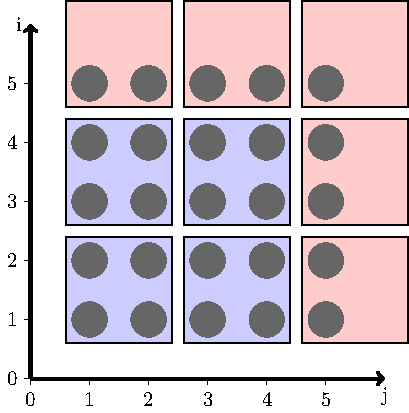
\includegraphics[width=0.8\textwidth]{figs/tile-2d_tiling}
\centering
\caption{2-dimensional tiling with partial tiles}\label{fig:2d_tiling}
\end{subfigure}%
\begin{subfigure}[b]{.5\textwidth}
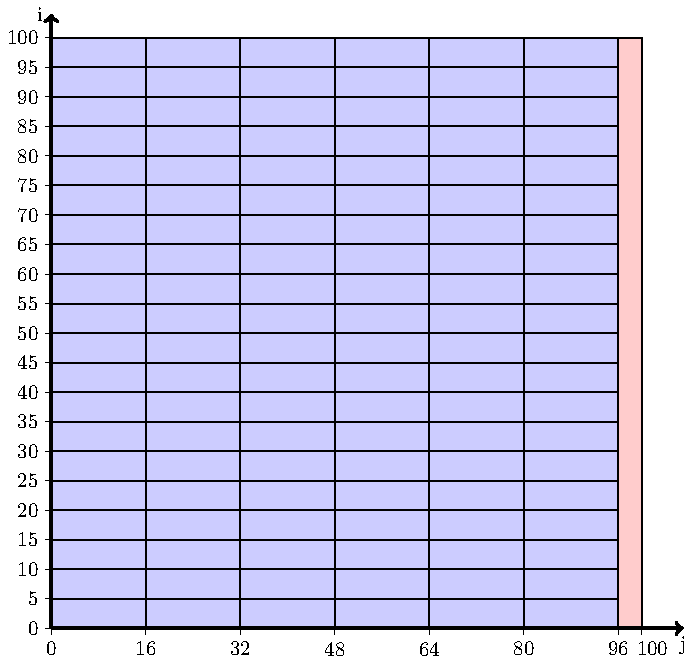
\includegraphics[width=0.85\textwidth]{figs/tile-Example_tile2}
\vspace*{2mm}
\centering
\caption{Partial tiles of Example \emph{partial\_tile.1}}\label{fig:Example_tile2}
\end{subfigure}
\caption{Tiling illustrations}
\end{figure}

In the following example, function \plc{func1} uses the \code{tile} construct
with a \code{sizes(4,16)} tiling clause.  Because the second tile dimension of
16 does not evenly divide into the iteration count of the j-loop, the
iterations corresponding to the remainder for the j-loop correspond to partial
tiles as shown in Figure~\ref{fig:Example_tile2}. Each remaining function
illustrates a code implementation that a compiler may generate to implement the
\code{tile} construct in \plc{func1}.

%Iterations with the tiles can be executed in a any order, ignoring partial tile boundaries.
% Deepak: I don't think this first sentence is true for iterations in a partial tile.
% Only the product order will be maintained for such iterations.
The order of tile execution relative to other tiles can be changed, but execution order of 
iterations within the same tile must be preserved.
Implementations must ensure that dependencies that are valid with any tile size need
to be preserved (including tile size of 1 and tiles as large as the iteration space).

Functions \plc{func2} through \plc{func6} are valid implementations of \plc{func1}.
In \splc{func2} the unrolling is illustrated as a pair of nested loops with a simple
adjustment in the size of the final iteration block in the \splc{j2} iteration space
for the partial tile.

Performance of the implementation depends on the hardware architecture, the instruction set and compiler optimization goals.
Functions \plc{func3}, \plc{func4}, and  \plc{func5} have the advantage that
the innermost loop for the complete tile is a constant size and can be replaced with SIMD instructions.
If the target platform has masked SIMD instructions with no overhead, then avoiding the construction of a
remainder loop, as in \plc{func5}, might be the best option.
Another option is to use a remainder loop without tiling, as shown in \plc{func6}, to reduce control-flow overhead.

\cexample[5.1]{partial_tile}{1}
\ffreeexample[5.1]{partial_tile}{1}


In the following example, function \plc{func7} tiles nested loops with a size of (4,16),
resulting in partial tiles that cover the last 4 iterations of the j-loop, as
in the previous example.  However, the outer loop is parallelized with a
\code{parallel} worksharing-loop construct.

Functions \plc{func8} and \plc{func9} illustrate two implementations of the tiling
with \code{parallel} and worksharing-loop directives.  Function \plc{func8} uses a single outer loop, with a \plc{min} function
to accommodate the partial tiles. Function \plc{func9}
uses two sets of nested loops, the first iterates over the complete tiles and the
second covers iterations from the partial tiles. When fissioning loops that
are in a \code{parallel} worksharing-loop region, each iteration of each workshared loop
must be executed on the same thread as in an un-fissioned loop.  The \code{schedule(static)} clause in \plc{func7}
forces the implementation to use static scheduling and allows the fission in function \plc{func8}.
When dynamic scheduling is prescribed, fissioning is not allowed.  When no scheduling is specified,
the compiler implementation will select a scheduling \plc{kind} and adhere to its restrictions.

\cexample[5.1]{partial_tile}{2}
\ffreeexample[5.1]{partial_tile}{2}



    \pagebreak
\chapter{Synchronization}
\label{chap:synchronization}

The \code{barrier} construct is a stand-alone directive that requires all threads
of a team (within a contention group) to execute the barrier and complete
execution of all tasks within the region, before continuing past the barrier.

The \code{critical} construct is a directive that contains a structured block. 
The construct allows only a single thread at a time to execute the structured block (region).
Multiple critical regions may exist in a parallel region, and may
act cooperatively (only one thread at a time in all \code{critical} regions),
or separately (only one thread at a time in each \code{critical} regions when
a unique name is supplied on each \code{critical} construct).
An optional (lock) \code{hint} clause may be specified on a named \code{critical} 
construct to provide the OpenMP runtime guidance in selection a locking 
mechanism.

On a finer scale the \code{atomic} construct allows only a single thread at 
a time to have atomic access to a storage location involving a single read, 
write, update or capture statement, and a limited number of combinations 
when specifying the \code{capture} \plc{atomic-clause} clause.  The
\plc{atomic-clause} clause is required for some expression statements, but is
not required for \code{update} statements. The \plc{memory-order} clause can be
used to specify the degree of memory ordering enforced by an \code{atomic}
construct. From weakest to strongest, they are \code{relaxed} (the default),
acquire and/or release clauses (specified with \code{acquire}, \code{release},
or \code{acq\_rel}), and \code{seq\_cst}.  Please see the details in the
\plc{atomic Construct} subsection of the \plc{Directives} chapter in the OpenMP
Specifications document.

% The following three sentences were stolen from the spec.
The \code{ordered} construct either specifies a structured block in a loop, 
simd, or loop SIMD region that will be executed in the order of the loop 
iterations.  The ordered construct sequentializes and orders the execution 
of ordered regions while allowing code outside the region to run in parallel.

Since OpenMP 4.5 the \code{ordered} construct can also be a stand-alone 
directive that specifies cross-iteration dependences in a doacross loop nest.  
The \code{depend} clause uses a \code{sink} \plc{dependence-type}, along with a 
iteration vector argument (vec) to indicate the iteration that satisfies the 
dependence.  The \code{depend} clause with a \code{source}
\plc{dependence-type} specifies dependence satisfaction.

The \code{flush} directive is a stand-alone construct for enforcing consistency
between a thread's view of memory and the view of memory for other threads (see
the Memory Model chapter of this document for more details). When the construct
is used with an explicit variable list, a \plc{strong flush} that forces a
thread's temporary view of memory to be consistent with the actual memory is
applied to all listed variables. When the construct is used without an explicit
variable list and without a \plc{memory-order} clause, a strong flush is
applied to all locally thread-visible data as defined by the base language, and
additionally the construct provides both acquire and release memory ordering
semantics.  When an explicit variable list is not present and a
\plc{memory-order} clause is present, the construct provides acquire and/or
release memory ordering semantics according to the \plc{memory-order} clause,
but no strong flush is performed. A resulting strong flush that applies to a
set of variables effectively ensures that no memory (load or store)
operation for the affected variables may be reordered across the \code{flush}
directive.

General-purpose routines provide mutual exclusion semantics through locks, 
represented by lock variables.  
The semantics allows a task to \plc{set}, and hence 
\plc{own} a lock, until it is \plc{unset} by the task that set it. A 
\plc{nestable} lock can be set multiple times by a task, and is used
when in code requires nested control of locks.  A \plc{simple lock} can
only be set once by the owning task. There are specific calls for the two
types of locks, and the variable of a specific lock type cannot be used by the
other lock type.  

Any explicit task will observe the synchronization prescribed in a 
\code{barrier} construct and an implied barrier.  Also, additional synchronizations 
are available for tasks.  All children of a task will wait at a \code{taskwait} (for 
their siblings to complete).  A \code{taskgroup} construct creates a region in which the
current task is suspended at the end of the region until all sibling tasks, 
and their descendants, have completed. 
Scheduling constraints on task execution can be prescribed by the \code{depend}
clause to enforce dependence on previously generated tasks.
More details on controlling task executions can be found in the \plc{Tasking} Chapter
in the OpenMP Specifications document. %(DO REF. RIGHT.)

    \cchapter{Data Environment}{data_environment}
\label{chap:data_environment}
The OpenMP \plc{data environment} contains data attributes of variables and
objects.  Many constructs (such as \kcode{parallel}, \kcode{simd}, \kcode{task}) 
accept clauses to control \plc{data-sharing} attributes
of referenced variables in the construct, where \plc{data-sharing} applies to
whether the attribute of the variable is \plc{shared}, 
is \plc{private} storage, or has special operational characteristics 
(as found in the \kcode{firstprivate}, \kcode{lastprivate}, \kcode{linear}, or \kcode{reduction} clause).

The data environment for a device (distinguished as a \plc{device data environment})
is controlled on the host by \plc{data-mapping} attributes, which determine the
relationship of the data on the host, the \plc{original} data, and the data on the
device, the \plc{corresponding} data.

\bigskip
DATA-SHARING ATTRIBUTES

Data-sharing attributes of variables can be classified as being \plc{predetermined},
\plc{explicitly determined} or \plc{implicitly determined}.

Certain variables and objects have predetermined attributes.  
A commonly found case is the loop iteration variable in associated loops 
of a \kcode{for} or \kcode{do} construct. It has a private data-sharing attribute.
Variables with predetermined data-sharing attributes cannot be listed in a data-sharing clause; but there are some
exceptions (mainly concerning loop iteration variables).

Variables with explicitly determined data-sharing attributes are those that are
referenced in a given construct and are listed in a data-sharing attribute
clause on the construct. Some of the common data-sharing clauses are:
\kcode{shared}, \kcode{private}, \kcode{firstprivate}, \kcode{lastprivate}, 
\kcode{linear}, and \kcode{reduction}. % Are these all of them?

Variables with implicitly determined data-sharing attributes are those
that are referenced in a given construct, do not have predetermined
data-sharing attributes, and are not listed in a data-sharing
attribute clause of an enclosing construct.
For a complete list of variables and objects with predetermined and
implicitly determined attributes, please refer to the
\docref{Data-sharing Attribute Rules for Variables Referenced in a Construct}
subsection of the OpenMP Specifications document.  

\bigskip
DATA-MAPPING ATTRIBUTES

The \kcode{map} clause on a device construct explicitly specifies how the list items in
the clause are mapped from the encountering task's data environment (on the host)
to the corresponding item in the device data environment (on the device).
The common \plc{list items} are arrays, array sections, scalars, pointers, and
structure elements (members). 

Procedures and global variables have predetermined data mapping if they appear
within the list or block of a \kcode{declare target} directive. Also, a C/C++ pointer
is mapped as a zero-length array section, as is a C++ variable that is a reference to a pointer.
% Waiting for response from Eric on this.

Without explicit mapping, non-scalar and non-pointer variables within the scope of the \kcode{target}
construct are implicitly mapped with a \plc{map-type} of \kcode{tofrom}.
Without explicit mapping, scalar variables within the scope of the \kcode{target}
construct are not mapped, but have an implicit firstprivate data-sharing
attribute. (That is, the value of the original variable is given to a private
variable of the same name on the device.) This behavior can be changed with
the \kcode{defaultmap} clause.

The \kcode{map} clause can appear on \kcode{target}, \kcode{target data} and 
\kcode{target enter/exit data} constructs.  The operations of creation and
removal of device storage as well as assignment of the original list item 
values to the corresponding list items may be complicated when the list 
item appears on multiple constructs or when the host and device storage 
is shared. In these cases the item's reference count, the number of times
it has been referenced (increment by 1 on entry and decrement by 1 on exit) in nested (structured)
map regions and/or accumulative (unstructured) mappings, determines the operation.
Details of the \kcode{map} clause and reference count operation are specified 
in the \docref{\kcode{map} Clause} subsection of the OpenMP Specifications document.


%===== Examples Sections =====
%\pagebreak
\section{\kcode{threadprivate} Directive}
\label{sec:threadprivate}
\index{directives!threadprivate@\kcode{threadprivate}}
\index{threadprivate directive@\kcode{threadprivate} directive}

The following examples demonstrate how to use the \kcode{threadprivate} directive 
 to give each thread a separate counter.

\cexample{threadprivate}{1}

\fexample{threadprivate}{1}

\pagebreak
\ccppspecificstart
The following example uses \kcode{threadprivate} on a static variable:

\cnexample{threadprivate}{2}

The following example demonstrates unspecified behavior for the initialization 
of a \kcode{threadprivate} variable. A \kcode{threadprivate}  variable is initialized 
once at an unspecified point before its first reference. Because \ucode{a} is 
constructed using the value of \ucode{x}  (which is modified by the statement 
\ucode{x++}), the value of \ucode{a.val}  at the start of the \kcode{parallel} 
region could be either 1 or 2. This problem is avoided for \ucode{b}, which uses 
an auxiliary \bcode{const} variable and a copy-constructor.

\cppnexample{threadprivate}{3}
\ccppspecificend

The following examples show non-conforming uses and correct uses of the \kcode{threadprivate} 
directive. 

\fortranspecificstart
The following example is non-conforming because the common block is not declared 
local to the subroutine that refers to it:

\fnexample{threadprivate}{2}

The following example is also non-conforming because the common block is not declared 
local to the subroutine that refers to it:

\fnexample{threadprivate}{3}

The following example is a correct rewrite of the previous example:

\fnexample{threadprivate}{4}

The following is an example of the use of \kcode{threadprivate} for local variables:
\topmarker{Fortran}

\fnexample{threadprivate}{5}

The above program, if executed by two threads, will print one of the following 
two sets of output: 

\pout{a = 11 12 13}
\\
\pout{ptr = 4}
\\
\pout{i = 15}

\pout{A is not allocated}
\\
\pout{ptr = 4}
\\
\pout{i = 5}

or

\pout{A is not allocated}
\\
\pout{ptr = 4}
\\
\pout{i = 15}

\pout{a = 1 2 3}
\\
\pout{ptr = 4}
\\
\pout{i = 5}

The following is an example of the use of \kcode{threadprivate} for module variables:
\topmarker{Fortran}

\fnexample{threadprivate}{6}
\fortranspecificend

\cppspecificstart
The following example illustrates initialization of \kcode{threadprivate} variables 
for class-type \ucode{T}. \ucode{t1} is default constructed, \ucode{t2} is constructed 
taking a constructor accepting one argument of integer type, \ucode{t3} is copy 
constructed with argument \ucode{f()}:

\cppnexample{threadprivate}{4}

The following example illustrates the use of \kcode{threadprivate} for static 
class members. The \kcode{threadprivate} directive for a static class member must 
be placed inside the class definition.

\cppnexample{threadprivate}{5}
\cppspecificend


\pagebreak
\section{\code{default(none)} Clause}
\label{sec:default_none}
\index{clauses!default(none)@\code{default(none)}}
\index{default(none) clause@\code{default(none)} clause}

The following example distinguishes the variables that are affected by the \code{default(none)} 
clause from those that are not. 

\ccppspecificstart
Beginning with OpenMP 4.0, variables with \code{const}-qualified type and no mutable member 
are no longer predetermined shared.  Thus, these variables (variable \plc{c} in the example) 
need to be explicitly listed
in data-sharing attribute clauses when the \code{default(none)} clause is specified.

\cnexample{default_none}{1}
\ccppspecificend

\fexample{default_none}{1}



\pagebreak
\section{\code{private} Clause}
\label{sec:private}
\index{clauses!private@\code{private}}
\index{private clause@\code{private} clause}

In the following example, the values of original list items \plc{i} and \plc{j} 
are retained on exit from the \code{parallel} region, while the private list 
items \plc{i} and \plc{j} are modified within the \code{parallel} construct. 

\cexample{private}{1}

\fexample{private}{1}

In the following example, all uses of the variable \plc{a} within the loop construct 
in the routine \plc{f} refer to a private list item \plc{a}, while it is 
unspecified whether references to \plc{a} in the routine \plc{g} are to a 
private list item or the original list item.

\cexample{private}{2}

\fexample{private}{2}

The following example demonstrates that a list item that appears in a \code{private} 
 clause in a \code{parallel} construct may also appear in a \code{private} 
 clause in an enclosed worksharing construct, which results in an additional private 
copy.

\cexample{private}{3}

\fexample{private}{3}



%\pagebreak
\section{Fortran Private Loop Iteration Variables}
\label{sec:fort_loopvar}
\fortranspecificstart
\index{loop variables, Fortran}

In general loop iteration variables will be private, when used in the \plc{do-loop} 
of a \kcode{do} and \kcode{parallel do} construct or in sequential loops in a 
\kcode{parallel} construct (see the \docref{Loop Construct} section and 
the \docref{Data-sharing Attribute Rules} section of 
the OpenMP 4.0 specification). In the following example of a sequential 
loop in a \kcode{parallel} construct the loop iteration variable \ucode{I} will 
be private.

\ffreenexample{fort_loopvar}{1}

In exceptional cases, loop iteration variables can be made shared, as in the following 
example:

\ffreenexample{fort_loopvar}{2}

Note however that the use of shared loop iteration variables can easily lead to 
race conditions.
\fortranspecificend


\pagebreak
\section{Fortran Restrictions on \code{shared} and \code{private} Clauses with Common Blocks}
\fortranspecificstart
\label{sec:fort_sp_common}
\index{clauses!private@\code{private}}
\index{clauses!shared@\code{shared}}
\index{private clause@\code{private} clause!common blocks, Fortran}
\index{shared clause@\code{shared} clause!common blocks, Fortran}

When a named common block is specified in a \code{private}, \code{firstprivate}, 
or \code{lastprivate} clause of a construct, none of its members may be declared 
in another data-sharing attribute clause on that construct. The following examples 
illustrate this point. 

The following example is conforming:

\fnexample{fort_sp_common}{1}

The following example is also conforming:

\fnexample{fort_sp_common}{2}
% blue line floater at top of this page for "Fortran, cont."
%\begin{figure}[t!]
%\linewitharrows{-1}{dashed}{Fortran (cont.)}{8em}
%\end{figure}
\clearpage

The following example is conforming:

\fnexample{fort_sp_common}{3}

The following example is non-conforming because \code{x} is a constituent element 
of \code{c}:

\fnexample{fort_sp_common}{4}

The following example is non-conforming because a common block may not be declared 
both shared and private:

\fnexample{fort_sp_common}{5}
\fortranspecificend



%\pagebreak
\begin{fortranspecific}[4ex]
\section{Fortran Restrictions on Storage Association with the \kcode{private} Clause}
\label{sec:fort_sa_private}
\index{clauses!private@\kcode{private}}
\index{private clause@\kcode{private} clause!storage association, Fortran}

The following non-conforming examples illustrate the implications of the \kcode{private} 
clause rules with regard to storage association. 

\pagebreak
\fnexample{fort_sa_private}{1}

\topmarker{Fortran}
\fnexample{fort_sa_private}{2}

\fnexample{fort_sa_private}{3}

\fnexample{fort_sa_private}{4}

\topmarker{Fortran}
\fnexample[5.1]{fort_sa_private}{5}
\end{fortranspecific}


%\pagebreak
\section{Passing Shared Variable to Procedure in Fortran}
\fortranspecificstart
\label{sec:fort_shared_var}
\index{clauses!shared@\kcode{shared}}
\index{shared clause@\kcode{shared} clause!storage association, Fortran}

Passing a shared variable to a procedure in Fortran may result in the use of
temporary storage in place of the actual argument when the corresponding dummy 
argument does not have the \bcode{VALUE} or \bcode{CONTIGUOUS} attribute and 
its data-sharing attribute is implementation-defined as per the rules in 
Section \docref{Variables Referenced in a Region but not in a Construct} of
the OpenMP Specification. 
These conditions effectively result in references to, and definitions of, the 
temporary storage during the procedure reference. Furthermore, the value of the 
shared variable is copied into the intervening temporary storage before the 
procedure reference when the dummy argument does not have the 
\bcode{INTENT(OUT)} attribute, and is copied out of the temporary storage into 
the shared variable when the dummy argument does not have the 
\bcode{INTENT(IN)} attribute. Any references to (or definitions of) the shared 
storage that is associated with the dummy argument by any other task must be 
synchronized with the procedure reference to avoid possible data races.

The following examples illustrate the implications of passing a shared 
variable \ucode{a} to subroutine \ucode{sub1} or \ucode{sub2} in
a \kcode{parallel} region.
For \ucode{sub1}, an implementation may or may not generate a copy-in/copy-out 
for the temporary storage associated with variable \ucode{b}. 
If there is a copy-in/copy-out, the code for copy-in/copy-out will result in 
a race condition, even though there is an \kcode{atomic}
directive for the update of variable \ucode{b(i)} in the subroutine. 
If the implementation can create a temporary descriptor for \ucode{a(::2)} 
with the correct stride and passed it to subroutine \ucode{sub1}, 
the same memory is accessed inside the subroutine and the result 
(\ucode{sum1}) is then well defined.
For \ucode{sub2}, there is the \bcode{CONTIGUOUS} attribute for 
variable \ucode{b} and the implementation will generate a copy-in/copy-out 
for the temporary storage.
The code will have a race condition and the result (\ucode{sum2}) is
not well defined.

\topmarker{Fortran}
\ffreenexample{fort_shared_var}{1}
\fortranspecificend


%\pagebreak
\section{C/C++ Arrays in a \kcode{firstprivate} Clause}
\ccppspecificstart
\label{sec:carrays_fpriv}
\index{clauses!firstprivate@\kcode{firstprivate}}
\index{firstprivate clause@\kcode{firstprivate} clause!C/C++ arrays in}

The following example illustrates the size and value of list items of array or 
pointer type in a \kcode{firstprivate} clause. The size of new list items is 
based on the type of the corresponding original list item, as determined by the 
base language.

In this example:

\begin{compactitem}
\item The type of \ucode{A} is array of two arrays of two \bcode{int}s.

\item  The type of \ucode{B} is adjusted to pointer to array of \ucode{n} 
\bcode{int}s, because it is a function parameter.

\item  The type of \ucode{C} is adjusted to pointer to \bcode{int}, because 
it is a function parameter.

\item  The type of \ucode{D} is array of two arrays of two \bcode{int}s.

\item  The type of \ucode{E} is array of \ucode{n} arrays of \ucode{n} 
\bcode{int}s.
\end{compactitem}

Note that  \ucode{B} and \ucode{E} involve variable length array types.

The new items of array type are initialized as if each integer element of the original 
array is assigned to the corresponding element of the new array. Those of pointer 
type are initialized as if by assignment from the original item to the new item.

\cnexample{carrays_fpriv}{1}
\ccppspecificend



%\pagebreak
\section{\kcode{lastprivate} Clause}
\label{sec:lastprivate}
\index{clauses!lastprivate@\kcode{lastprivate}}
\index{lastprivate clause@\kcode{lastprivate} clause}

Correct execution sometimes depends on the value that the last iteration of a loop 
assigns to a variable. Such programs must list all such variables in a \kcode{lastprivate} 
clause  so that the values of the variables are the same as when the loop is executed 
sequentially.

\cexample{lastprivate}{1}

\fexample{lastprivate}{1}

\index{lastprivate clause@\kcode{lastprivate} clause!conditional modifier@\kcode{conditional} modifier}
\index{conditional modifier@\kcode{conditional} modifier}
The next example illustrates the use of the \kcode{conditional} modifier in
a \kcode{lastprivate} clause to return the last value when it may not come from
the last iteration of a loop.
That is, users can preserve the serial equivalence semantics of the loop.
The conditional lastprivate ensures the final value of the variable after the loop 
is as if the loop iterations were executed in a sequential order.

\cexample[5.0]{lastprivate}{2}

\ffreeexample[5.0]{lastprivate}{2}

\pagebreak

\section{Reduction}
\label{sec:reduction}

This section covers ways to perform reductions in parallel, task, taskloop, and SIMD regions.

\subsection{\code{reduction} Clause}
\label{subsec:reduction}
\index{clauses!reduction@\code{reduction}}
\index{reduction clause@\code{reduction} clause}
\index{reductions!reduction clause@\code{reduction} clause}

The following example demonstrates the \code{reduction} clause; note that some 
reductions can be expressed in the loop in several ways, as shown for the \code{max} 
and \code{min} reductions below:

\cexample[3.1]{reduction}{1}

\pagebreak

\ffreeexample{reduction}{1}

A common implementation of the preceding example is to treat it as if it had been 
written as follows:

\cexample{reduction}{2}

\fortranspecificstart
\ffreenexample{reduction}{2}

The following program is non-conforming because the reduction is on the 
\emph{intrinsic procedure name} \code{MAX} but that name has been redefined to be the variable 
named \code{MAX}.

\ffreenexample{reduction}{3}
% blue line floater at top of this page for "Fortran, cont."
\begin{figure}[t!]
\linewitharrows{-1}{dashed}{Fortran (cont.)}{8em}
\end{figure}

The following conforming program performs the reduction using the 
\emph{intrinsic procedure name} \code{MAX} even though the intrinsic \code{MAX} has been renamed 
to \code{REN}.

\ffreenexample{reduction}{4}

The following conforming program performs the reduction using 
\plc{intrinsic procedure name} \code{MAX} even though the intrinsic \code{MAX} has been renamed 
to \code{MIN}.

\ffreenexample{reduction}{5}
\fortranspecificend

%\pagebreak
The following example is non-conforming because the initialization (\code{a = 
0}) of the original list item \code{a} is not synchronized with the update of 
\code{a} as a result of the reduction computation in the \code{for} loop. Therefore, 
the example may print an incorrect value for \code{a}.

To avoid this problem, the initialization of the original list item \code{a} 
should complete before any update of \code{a} as a result of the \code{reduction} 
clause. This can be achieved by adding an explicit barrier after the assignment 
\code{a = 0}, or by enclosing the assignment \code{a = 0} in a \code{single} 
directive (which has an implied barrier), or by initializing \code{a} before 
the start of the \code{parallel} region.

\cexample[5.1]{reduction}{6}

\fexample[5.1]{reduction}{6}

The following example demonstrates the reduction of array \plc{a}.  In C/C++ this is illustrated by the explicit use of an array section \plc{a[0:N]} in the \code{reduction} clause.  The corresponding Fortran example uses array syntax supported in the base language.  As of the OpenMP 4.5 specification the explicit use of array section in the \code{reduction} clause in Fortran is not permitted.  But this oversight has been fixed in the OpenMP 5.0 specification.


\cexample[4.5]{reduction}{7}

\ffreeexample{reduction}{7}

\subsection{Task Reduction}
\label{subsec:task_reduction}
\index{clauses!task_reduction@\scode{task_reduction}}
\index{task_reduction clause@\scode{task_reduction} clause}
\index{reductions!task_reduction clause@\scode{task_reduction} clause}
\index{clauses!in_reduction@\scode{in_reduction}}
\index{in_reduction clause@\scode{in_reduction} clause}
\index{reductions!in_reduction clause@\scode{in_reduction} clause}

In OpenMP 5.0 the \code{task\_reduction} clause was created for the \code{taskgroup} construct, 
to allow reductions among explicit tasks that have an \code{in\_reduction} clause.

In the \plc{task\_reduction.1} example below a reduction is performed as the algorithm
traverses a linked list. The reduction statement is assigned to be an explicit task using
a \code{task} construct and is specified to be a reduction participant with 
the \code{in\_reduction} clause.
A \code{taskgroup} construct encloses the tasks participating in the reduction, and
specifies, with the \code{task\_reduction} clause, that the taskgroup has tasks participating
in a reduction.  After the \code{taskgroup} region the original variable will contain 
the final value of the reduction.

Note: The \plc{res} variable is private in the \plc{linked\_list\_sum} routine
and is not required to be shared (as in the case of a \code{parallel} construct
reduction).


\cexample[5.0]{task_reduction}{1}

\ffreeexample[5.0]{task_reduction}{1}

\index{reduction clause@\code{reduction} clause!task modifier@\code{task} modifier}
\index{task modifier@\code{task} modifier}
In OpenMP 5.0 the \code{task} \plc{reduction-modifier} for the \code{reduction} clause was
introduced to provide a means of performing reductions among implicit and explicit tasks.

The \code{reduction} clause of a \code{parallel} or worksharing construct may
specify the \code{task} \plc{reduction-modifier} to include explicit task reductions
within their region, provided the reduction operators (\plc{reduction-identifiers})
and variables (\plc{list items}) of the participating tasks match those of the
implicit tasks.

There are 2 reduction use cases (identified by USE CASE \#) in the \plc{task\_reduction.2} example below.  

In USE CASE 1 a \code{task} modifier in the \code{reduction} clause 
of the \code{parallel} construct is used to include the reductions of any 
participating tasks, those with an \code{in\_reduction} clause and matching 
\plc{reduction-identifiers} (\code{+}) and list items (\code{x}).  

Note, a \code{taskgroup} construct (with a \code{task\_reduction} clause) in not
necessary to scope the explicit task reduction (as seen in the example above). 
Hence, even without the implicit task reduction statement (without the C \code{x++\;}  
and Fortran \code{x=x+1} statements), the \code{task} \plc{reduction-modifier} 
in a \code{reduction} clause of the \code{parallel} construct
can be used to avoid having to create a \code{taskgroup} construct 
(and its \code{task\_reduction} clause) around the task generating structure.

In USE CASE 2 tasks participating in the reduction are within a
worksharing region (a parallel worksharing-loop construct).
Here, too, no \code{taskgroup} is required, and the \plc{reduction-identifier} (\code{+})
and list item (variable \code{x}) match as required.


\cexample[5.0]{task_reduction}{2}

\ffreeexample[5.0]{task_reduction}{2}


\subsection{Reduction on Combined Target Constructs}
\label{subsec:target_reduction}
\index{reduction clause@\code{reduction} clause!on target construct@on \code{target} construct}
\index{constructs!target@\code{target}}
\index{target construct@\code{target} construct}

When a \code{reduction} clause appears on a combined construct that combines 
a \code{target} construct with another construct, there is an implicit map 
of the list items with a \code{tofrom} map type for the \code{target} construct. 
Otherwise, the list items (if they are scalar variables) would be 
treated as firstprivate by default in the \code{target} construct, which 
is unlikely to provide the intended behavior since the result of the
reduction that is in the firstprivate variable would be discarded 
at the end of the \code{target} region.

In the following example, the use of the \code{reduction} clause on \code{sum1}
or \code{sum2} should, by default, result in an implicit \code{tofrom} map for
that variable. So long as neither \code{sum1} nor \code{sum2} were already
present on the device, the mapping behavior ensures the value for
\code{sum1} computed in the first \code{target} construct is used in the
second \code{target} construct.

\cexample[5.0]{target_reduction}{1}

\ffreeexample[5.0]{target_reduction}{1}
%\clearpage

In next example,  the variables \code{sum1} and \code{sum2} remain on the
device for the duration of the \code{target}~\code{data} region so that it is
their device copies that are updated by the reductions. Note the significance
of mapping \code{sum1} on the second \code{target} construct; otherwise, it
would be treated by default as firstprivate and the result computed for
\code{sum1} in the prior \code{target} region may not be used. Alternatively, a
\code{target}~\code{update} construct could be used between the two
\code{target} constructs to update the host version of \code{sum1} with the
value that is in the corresponding device version after the completion of the
first construct.

\cexample[5.0]{target_reduction}{2}

\ffreeexample[5.0]{target_reduction}{2}


\subsection{Task Reduction with Target Constructs}
\label{subsec:target_task_reduction}
\index{in_reduction clause@\scode{in_reduction} clause}
\index{constructs!target@\code{target}}
\index{target construct@\code{target} construct}

\index{clauses!enter@\code{enter}}
\index{enter clause@\code{enter} clause}

The following examples illustrate how task reductions can apply to target tasks
that result from a \code{target} construct with the \code{in\_reduction}
clause. Here, the \code{in\_reduction} clause specifies that the target task
participates in the task reduction defined in the scope of the enclosing
\code{taskgroup} construct. Partial results from all tasks participating in the
task reduction will be combined (in some order) into the original variable
listed in the \code{task\_reduction} clause before exiting the \code{taskgroup}
region. 

\cexample[5.2]{target_task_reduction}{1}

\ffreeexample[5.2]{target_task_reduction}{1}
\clearpage

\index{reduction clause@\code{reduction} clause!task modifier@\code{task} modifier}
\index{task modifier@\code{task} modifier}
In the next pair of examples, the task reduction is defined by a
\code{reduction} clause with the \code{task} modifier, rather than a
\code{task\_reduction} clause on a \code{taskgroup} construct. Again, the
partial results from the participating tasks will be combined in some order
into the original reduction variable, \code{sum}.

\cexample[5.2]{target_task_reduction}{2a}

\ffreeexample[5.2]{target_task_reduction}{2a}

\index{in_reduction clause@\scode{in_reduction} clause!with target construct@with \code{target} construct}
\index{constructs!target@\code{target}}
\index{target construct@\code{target} construct}
Next, the \code{task} modifier is again used to define a task reduction over
participating tasks. This time, the participating tasks are a target task
resulting from a \code{target} construct with the \code{in\_reduction} clause,
and the implicit task (executing on the primary thread) that calls
\code{host\_compute}. As before, the partial results from these participating
tasks are combined in some order into the original reduction variable.

\cexample[5.2]{target_task_reduction}{2b}

\ffreeexample[5.2]{target_task_reduction}{2b}


\subsection{Taskloop Reduction}
\label{subsec:taskloop_reduction}
\index{reduction clause@\code{reduction} clause!on taskloop construct@on \code{taskloop} construct}
\index{constructs!taskloop@\code{taskloop}}
\index{taskloop construct@\code{taskloop} construct}

In the OpenMP 5.0 Specification the \code{taskloop} construct
was extended to include the reductions.

The following two examples show how to implement a reduction over an array
using taskloop reduction in two different ways.
In the first
example we apply the \code{reduction} clause to the \code{taskloop} construct. As it was
explained above in the task reduction examples, a reduction over tasks is
divided in two components: the scope of the reduction, which is defined by a
\code{taskgroup} region, and the tasks that participate in the reduction. In this
example, the \code{reduction} clause defines both semantics. First, it specifies that
the implicit \code{taskgroup} region associated with the \code{taskloop} construct is the scope of the
reduction, and second, it defines all tasks created by the \code{taskloop} construct as
participants of the reduction. About the first property, it is important to note
that if we add the \code{nogroup} clause to the \code{taskloop} construct the code will be
nonconforming, basically because we have a set of tasks that participate in a
reduction that has not been defined.

\cexample[5.0]{taskloop_reduction}{1}
\ffreeexample[5.0]{taskloop_reduction}{1}

%In the second example, we are computing exactly the same
%value but we do it in a very different way. The first thing that we do in the
%\plc{array\_sum} function is to create a \code{taskgroup} region that defines the scope of a
%new reduction using the \code{task\_reduction} clause.
%After that, we specify that a task and also the tasks generated
%by a taskloop will participate in that reduction using the \code{in\_reduction} clause
%on the \code{task} and \code{taskloop} constructs, respectively. Note that
%we also added the \code{nogroup} clause to the \code{taskloop} construct. This is allowed
%because what we are expressing with the \code{in\_reduction} clause is different
%from what we were expressing with the \code{reduction} clause. In one case we specify
%that the generated tasks will participate in a previously declared reduction
%(\code{in\_reduction} clause) whereas in the other case we specify that we want to
%create a new reduction and also that all tasks generated by the taskloop will
%participate on it.

The second example computes exactly the same value as in the preceding \plc{taskloop\_reduction.1} code section,
but in a very different way.
First, in the \plc{array\_sum} function a \code{taskgroup} region is created 
that defines the scope of a new reduction using the \code{task\_reduction} clause.
After that, a task and also the tasks generated by a taskloop participate in 
that reduction by using the \code{in\_reduction} clause on the \code{task}
and \code{taskloop} constructs, respectively. 
Note that the \code{nogroup} clause was added to the \code{taskloop} construct.
This is allowed because what is expressed with the \code{in\_reduction} clause
is different from what is expressed with the \code{reduction} clause.
In one case the generated tasks are specified to participate in a previously 
declared reduction (\code{in\_reduction} clause) whereas in the other case
creation of a new reduction is specified and also all tasks generated 
by the taskloop will participate on it.

\cexample[5.0]{taskloop_reduction}{2}
\ffreeexample[5.0]{taskloop_reduction}{2}
%\clearpage

In the OpenMP 5.0 Specification, \code{reduction} clauses for the
\code{taskloop}~\code{ simd} construct were also added. 

\index{reduction clause@\code{reduction} clause!on taskloop simd construct@on \code{taskloop}~\code{simd} construct}
\index{combined constructs!taskloop simd@\code{taskloop}~\code{simd}}
\index{taskloop simd construct@\code{taskloop}~\code{simd} construct}
The examples below compare reductions for the \code{taskloop} and the \code{taskloop}~\code{simd} constructs.
These examples illustrate the use of \code{reduction} clauses within 
"stand-alone" \code{taskloop} constructs, and the use of \code{in\_reduction} clauses for tasks of taskloops to participate
with other reductions within the scope of a parallel region.

\textbf{taskloop reductions:}

In the \plc{taskloop reductions} section of the example below, 
\plc{taskloop 1} uses the \code{reduction} clause 
in a \code{taskloop} construct for a sum reduction, accumulated in \plc{asum}. 
The behavior is as though a \code{taskgroup} construct encloses the 
taskloop region with a \code{task\_reduction} clause, and each taskloop
task has an \code{in\_reduction} clause with the specifications 
of the \code{reduction} clause.
At the end of the taskloop region \plc{asum} contains the result of the reduction.

The next taskloop, \plc{taskloop 2}, illustrates the use of the 
\code{in\_reduction} clause to participate in a previously defined
reduction scope of a \code{parallel} construct.

The task reductions of \plc{task 2} and \plc{taskloop 2} are combined
across the \code{taskloop} construct and the single \code{task} construct, as specified
in the \code{reduction(task,}~\code{+:asum)} clause of the \code{parallel} construct.
At the end of the parallel region \plc{asum} contains the combined result of all reductions.

\textbf{taskloop simd reductions:}

Reductions for the \code{taskloop}~\code{simd} construct are shown in the second half of the code.
Since each component construct, \code{taskloop} and \code{simd}, 
can accept a reduction-type clause, the \code{taskloop}~\code{simd} construct
is a composite construct, and the specific application of the reduction clause is defined
within the \code{taskloop}~\code{simd} construct section of the OpenMP 5.0 Specification.
The code below illustrates use cases for these reductions.

In the \plc{taskloop simd reduction} section of the example below,
\plc{taskloop simd 3} uses the \code{reduction} clause 
in a \code{taskloop}~\code{simd} construct for a sum reduction within a loop.
For this case a \code{reduction} clause is used, as one would use 
for a \code{simd} construct.
The SIMD reductions of each task are combined, and the results of these tasks are further 
combined just as in the \code{taskloop} construct with the \code{reduction} clause for \plc{taskloop 1}.
At the end of the taskloop region \plc{asum} contains the combined result of all reductions.

If a \code{taskloop}~\code{simd} construct is to participate in a previously defined 
reduction scope, the reduction participation should be specified with
a \code{in\_reduction} clause, as shown in the \code{parallel} region enclosing
\plc{task 4} and \plc{taskloop simd 4} code sections.  

Here the \code{taskloop}~\code{simd} construct's 
\code{in\_reduction} clause specifies participation of the construct's tasks as 
a task reduction within the scope of the parallel region.  
That is, the results of each task of the \code{taskloop} construct component 
contribute to the reduction in a broader level, just as in \plc{parallel reduction a} code section above.
Also, each \code{simd}-component construct
occurs as if it has a \code{reduction} clause, and the
SIMD results of each task are combined as though to form a single result for
each task (that participates in the \code{in\_reduction} clause).
At the end of the parallel region \plc{asum} contains the combined result of all reductions.

%Just as in \plc{parallel reduction a} the
%\code{taskloop simd} construct reduction results are combined 
%with the \code{task} construct reduction results
%as specified by the \code{in\_reduction} clause of the \code{task} construct
%and the \plc{task} reduction-modifier of the \code{reduction} clause of 
%the \code{parallel} construct.
%At the end of the parallel region \plc{asum} contains the combined result of all reductions.


\cexample[5.1]{taskloop_simd_reduction}{1}

\ffreeexample[5.1]{taskloop_simd_reduction}{1}


\subsection{Reduction with the \code{scope} Construct}
\label{subsec:reduction_scope}
\index{reduction clause@\code{reduction} clause!on scope construct@on \code{scope} construct}
\index{constructs!scope@\code{scope}}
\index{scope construct@\code{scope} construct}

The following example illustrates the use of the \code{scope} construct 
to perform a reduction in a \code{parallel} region. The case is useful for 
producing a reduction and accessing reduction variables inside a \code{parallel} region 
without using a worksharing-loop construct.

\cppexample[5.1]{scope_reduction}{1}
\clearpage

\ffreeexample[5.1]{scope_reduction}{1}


\subsection{User-Defined Reduction}
\label{subsec:UDR}
\index{reductions!user-defined}
\index{reductions!declare reduction directive@\code{declare}~\code{reduction} directive}
\index{declare reduction directive@\code{declare}~\code{reduction} directive}
\index{directives!declare reduction@\code{declare}~\code{reduction}}
\index{declare reduction directive@\code{declare}~\code{reduction} directive!initializer clause@\code{initializer} clause}
\index{declare reduction directive@\code{declare}~\code{reduction} directive!combiner}
\index{declare reduction directive@\code{declare}~\code{reduction} directive!OpenMP variable identifiers}
\index{OpenMP variable identifiers!omp_in@\scode{omp_in}}
\index{OpenMP variable identifiers!omp_out@\scode{omp_out}}
\index{OpenMP variable identifiers!omp_priv@\scode{omp_priv}}
\index{combiner}
\index{clauses!initializer@\code{initializer}}
\index{initializer clause@\code{initializer} clause}

The \code{declare}~\code{reduction} directive can be used to specify 
user-defined reductions (UDR) for user data types.

%The following examples show how user-defined reductions can be used to support user data types in the \code{reduction} clause.

%The following example computes the enclosing rectangle of a set of points. The point data structure (\code{struct}~\code{point}) is not supported by the \code{reduction} clause. Using two \code{declare}~\code{reduction} directives we define how a reduction for the point data structure is done for the \plc{min} and \plc{max} operations. Each \code{declare}~\code{reduction} directive calls the appropriate function that passes the two special variables that can be used in the user-defined reduction expression: \code{omp\_in}, which holds one of the two values to reduce, and \code{omp\_out}, which holds the other value and should hold also the result of the reduction once the expression has been executed. Note, also, that when defining the user-defined reduction for \plc{min} we specify how the private variables of each thread are to be initialized (that is, the neutral value). This is not the case for \plc{max} as the default values (that is, zero filling) are already adequate.


In the following example, \code{declare}~\code{reduction} directives are used to define
\plc{min} and \plc{max} operations for the \plc{point} data structure for computing
the rectangle that encloses a set of 2-D points.

Each \code{declare}~\code{reduction} directive defines new reduction identifiers,
\plc{min} and \plc{max}, to be used in a \code{reduction} clause. The next item in the
declaration list is the data type (\plc{struct} \plc{point}) used in the reduction,
followed by the combiner, here the functions \plc{minproc} and \plc{maxproc} perform
the min and max operations, respectively, on the user data (of type \plc{struct} \plc{point}).
In the function argument list are two special OpenMP variable identifiers, \code{omp\_in} and \code{omp\_out},
that denote the two values to be combined in the "real" function;
the \code{omp\_out} identifier indicates which one is to hold the result.

The initializer of the \code{declare}~\code{reduction} directive specifies
the initial value for the private variable of each implicit task.
The \code{omp\_priv} identifier is used to denote the private variable.

\cexample[4.0]{udr}{1}
%\clearpage

The following example shows the corresponding code in Fortran. 
The \code{declare}~\code{reduction} directives are specified as part of 
the declaration in subroutine \plc{find\_enclosing\_rectangle} and 
the procedures that perform the min and max operations are specified as subprograms.

\ffreeexample[4.0]{udr}{1}


The following example shows the same computation as \plc{udr.1} but it illustrates that you can craft complex expressions in the user-defined reduction declaration. In this case, instead of calling the \plc{minproc} and \plc{maxproc} functions we inline the code in a single expression.

\cexample[4.0]{udr}{2}

The corresponding code of the same example in Fortran is very similar
except that the assignment expression in the \code{declare}~\code{reduction}
directive can only be used for a single variable, in this case through
a type structure constructor \plc{point($\ldots$)}.

\ffreeexample[4.0]{udr}{2}


\index{OpenMP variable identifiers!omp_orig@\scode{omp_orig}}
The following example shows the use of special variables in arguments for combiner (\code{omp\_in} and \code{omp\_out}) and initializer (\code{omp\_priv} and \code{omp\_orig}) routines.  This example returns the maximum value of an array and the corresponding index value. The \code{declare}~\code{reduction} directive specifies a user-defined reduction operation \plc{maxloc} for data type \plc{struct} \plc{mx\_s}. The function \plc{mx\_combine} is the combiner and the function \plc{mx\_init} is the initializer.

\cexample[4.0]{udr}{3}

Below is the corresponding Fortran version of the above example.  The \code{declare}~\code{reduction} directive specifies the user-defined operation \plc{maxloc} for user-derived type \plc{mx\_s}.  The combiner \plc{mx\_combine} and the initializer \plc{mx\_init} are specified as subprograms.

\ffreeexample[4.0]{udr}{3}


The following example explains a few details of the user-defined reduction 
in Fortran through modules. The \code{declare}~\code{reduction} directive is declared in a module (\plc{data\_red}). 
The reduction-identifier \plc{.add.} is a user-defined operator that is
to allow accessibility in the scope that performs the reduction
operation.
The user-defined operator \plc{.add.} and the subroutine \plc{dt\_init} specified in the \code{initializer} clause are defined in the same subprogram.

The reduction operation (that is, the \code{reduction} clause) is in the main program.
The reduction identifier \plc{.add.} is accessible by use association.
Since \plc{.add.} is a user-defined operator, the explicit interface
should also be accessible by use association in the current
program unit.
Since the \code{declare}~\code{reduction} associated to this \code{reduction} clause
has the \code{initializer} clause, the subroutine specified on the clause
must be accessible in the current scoping unit.  In this case,
the subroutine \plc{dt\_init} is accessible by use association.

\ffreeexample[4.0]{udr}{4}


The following example uses user-defined reductions to declare a plus (+) reduction for a C++ class. As the \code{declare}~\code{reduction} directive is inside the context of the \plc{V} class the expressions in the \code{declare}~\code{reduction} directive are resolved in the context of the class. Also, note that the \code{initializer} clause uses a copy constructor to initialize the private variables of the reduction and it uses as parameter to its original variable by using the special variable \code{omp\_orig}.

\cppexample[4.0]{udr}{5}

The following examples shows how user-defined reductions can be defined for some STL containers. The first \code{declare}~\code{reduction} defines the plus (+) operation for \plc{std::vector<int>} by making use of the \plc{std::transform} algorithm. The second and third define the merge (or concatenation) operation for \plc{std::vector<int>} and \plc{std::list<int>}. 
%It shows how the same user-defined reduction operation can be defined to be done differently depending on the specified data type.
It shows how the user-defined reduction operation can be applied to specific data types of an STL.

\cppexample[4.0]{udr}{6}


%\pagebreak
\section{\kcode{scan} Directive}
\label{sec:scan}
\index{directives!scan@\kcode{scan}}
\index{scan directive@\kcode{scan} directive}
\index{reduction clause@\kcode{reduction} clause!inscan modifier@\kcode{inscan} modifier}
\index{inscan modifier@\kcode{inscan} modifier}

The following examples illustrate how to parallelize a loop that saves 
the \emph{prefix sum} of a reduction. This is accomplished by using 
the \kcode{inscan} modifier in the \kcode{reduction} clause for the input 
variable of the scan, and specifying with a \kcode{scan} directive whether 
the storage statement includes or excludes the scan input of the present 
iteration (\ucode{k}).

\index{scan directive@\kcode{scan} directive!inclusive clause@\kcode{inclusive} clause}
\index{scan directive@\kcode{scan} directive!exclusive clause@\kcode{exclusive} clause}
\index{clauses!inclusive@\kcode{inclusive}}
\index{inclusive clause@\kcode{inclusive} clause}
\index{clauses!exclusive@\kcode{exclusive}}
\index{exclusive clause@\kcode{exclusive} clause}
Basically, the \kcode{inscan} modifier connects a loop and/or SIMD reduction to 
the scan operation, and a \kcode{scan} construct with an \kcode{inclusive} or 
\kcode{exclusive} clause specifies whether the ``scan phase'' (lexical block 
before and after the directive, respectively) is to use an \plc{inclusive} or 
\plc{exclusive} scan value for the list item (\ucode{x}).

The first example uses the \plc{inclusive} scan operation on a composite
loop-SIMD construct. The \kcode{scan} directive separates the reduction 
statement on variable \ucode{x} from the use of \ucode{x} (saving to array \ucode{b}).
The order of the statements in this example indicates that
value \ucode{a[k]} (\ucode{a(k)} in Fortran) is included in the computation of 
the prefix sum \ucode{b[k]} (\ucode{b(k)} in Fortran) for iteration \ucode{k}.

\cexample[5.0]{scan}{1}

\ffreeexample[5.0]{scan}{1}

The second example uses the \plc{exclusive} scan operation on a composite
loop-SIMD construct. The \kcode{scan} directive separates the use of \ucode{x} 
(saving to array \ucode{b}) from the reduction statement on variable \ucode{x}.
The order of the statements in this example indicates that
value \ucode{a[k]} (\ucode{a(k)} in Fortran) is excluded from the computation 
of the prefix sum \ucode{b[k]} (\ucode{b(k)} in Fortran) for iteration \ucode{k}.

\cexample[5.0]{scan}{2}

\ffreeexample[5.0]{scan}{2}

%\pagebreak
\section{\kcode{copyin} Clause}
\label{sec:copyin}
\index{clauses!copyin@\kcode{copyin}}
\index{copyin clause@\kcode{copyin} clause}
\index{directives!threadprivate@\kcode{threadprivate}}
\index{threadprivate directive@\kcode{threadprivate} directive}

The \kcode{copyin} clause is used to initialize threadprivate data upon entry 
to a \kcode{parallel} region. The value of the threadprivate variable in the primary
thread is copied to the threadprivate variable of each other team member.

\cexample{copyin}{1}

\fexample{copyin}{1}



%\pagebreak
\section{\kcode{copyprivate} Clause}
\label{sec:copyprivate}
\index{clauses!copyprivate@\kcode{copyprivate}}
\index{copyprivate clause@\kcode{copyprivate} clause}

The \kcode{copyprivate} clause can be used to broadcast values acquired by a single 
thread directly to all instances of the private variables in the other threads. 
In this example, if the routine is called from the sequential part, its behavior 
is not affected by the presence of the directives. If it is called from a \kcode{parallel} 
region, then the actual arguments with which \ucode{a} and \ucode{b} are associated 
must be private. 

\index{constructs!single@\kcode{single}}
\index{single construct@\kcode{single} construct}
The thread that executes the structured block associated with the \kcode{single} 
 construct broadcasts the values of the private variables \ucode{a}, \ucode{b}, 
\ucode{x}, and 
\ucode{y} from its implicit task's data environment to the data environments 
of the other implicit tasks in the thread team. The broadcast completes before 
any of the threads have left the barrier at the end of the construct.

\cexample{copyprivate}{1}

\fexample{copyprivate}{1}

\index{constructs!masked@\kcode{masked}}
\index{masked construct@\kcode{masked} construct}
In this example, assume that the input must be performed by the primary thread. 
Since the \kcode{masked} construct does not support the \kcode{copyprivate} clause, 
it cannot broadcast the input value that is read. However, \kcode{copyprivate} 
is used to broadcast an address where the input value is stored. 

\cexample[5.1]{copyprivate}{2}

\fexample[5.1]{copyprivate}{2}

Suppose that the number of lock variables required within a \kcode{parallel} region 
cannot easily be determined prior to entering it. The \kcode{copyprivate} clause 
can be used to provide access to shared lock variables that are allocated within 
that \kcode{parallel} region.

\cexample{copyprivate}{3}

\begin{fortranspecific}
\fnexample{copyprivate}{3}

Note that the effect of the \kcode{copyprivate} clause on a variable with the 
\bcode{allocatable} attribute is different than on a variable with the \bcode{pointer} 
attribute. The value of \ucode{A} is copied (as if by intrinsic assignment) and 
the pointer \ucode{B} is copied (as if by pointer assignment) to the corresponding 
list items in the other implicit tasks belonging to the \kcode{parallel} region. 

\fnexample{copyprivate}{4}
\end{fortranspecific}



\begin{cppspecific}[4ex]
\section{C++ Reference in Data-Sharing Clauses}
\label{sec:cpp_reference}
\index{clauses!data-sharing, C++ reference in}
\index{data-sharing clauses, C++ reference in}

C++ reference types are allowed in data-sharing attribute clauses as of OpenMP 4.5, except
for the \kcode{threadprivate}, \kcode{copyin} and \kcode{copyprivate} clauses.  
(See the \docref{Data-Sharing Attribute Clauses} section of the 4.5 OpenMP specification.)
When a variable with C++ reference type is privatized, the object the reference refers to is privatized in addition to the reference itself.
The following example shows the use of reference types in data-sharing clauses in the usual way.
Additionally it shows how the data-sharing of formal arguments with a C++ reference type on an orphaned task generating construct is determined implicitly. (See the \docref{Data-sharing Attribute Rules for Variables Referenced in a Construct} section of the 4.5 OpenMP specification.)


\cppnexample[4.5]{cpp_reference}{1}
\end{cppspecific}

\pagebreak
\section{Fortran \code{ASSOCIATE} Construct}
\fortranspecificstart
\label{sec:associate}
\index{ASSOCIATE construct, Fortran@\code{ASSOCIATE} construct, Fortran}

The following is an invalid example of specifying an associate name on a data-sharing attribute 
clause. The constraint in the Data Sharing Attribute Rules section in the OpenMP 
4.0 API Specifications states that an associate name preserves the association 
with the selector established at the \code{ASSOCIATE} statement. The associate 
name \plc{b} is associated with the shared variable \plc{a}. With the predetermined data-sharing 
attribute rule, the associate name \plc{b} is not allowed to be specified on the \code{private} 
clause.

\fnexample[4.0]{associate}{1}

In next example, within the \code{parallel} construct, the association name \plc{thread\_id} 
is associated with the private copy of \plc{i}. The print statement should output the 
unique thread number.

\fnexample[4.0]{associate}{2}

The following example illustrates the effect of specifying a selector name on a data-sharing 
attribute clause. The associate name \plc{u} is associated with \plc{v} and the variable \plc{v} 
is specified on the \code{private} clause of the \code{parallel} construct. 
The construct association is established prior to the \code{parallel} region. 
The association between \plc{u} and the original \plc{v} is retained (see the Data Sharing 
Attribute Rules section in the OpenMP 4.0 API Specifications). Inside the \code{parallel} 
region, \plc{v} has the value of -1 and \plc{u} has the value of the original \plc{v}.

\pagebreak
\ffreenexample[4.0]{associate}{3}

% blue line floater at top of this page for "Fortran, cont."
\begin{figure}[t!]
\linewitharrows{-1}{dashed}{Fortran (cont.)}{8em}
\end{figure}
\label{sec:associate_target}

\bigskip
The following example illustrates mapping behavior for a Fortran
associate name and its selector for a \scode{target} construct.

For the first 3 \scode{target} constructs the associate name \splc{a_aray} is
associated with the selector \splc{aray}, an array.  
For the \scode{target} construct of code block TARGET 1 just the selector
\splc{aray} is used and is implicitly mapped,
likewise for the associate name \splc{a_aray} in the TARGET 2 block.  
However, mapping an associate name and its selector is not valid for the same
\scode{target} construct.  Hence the TARGET 3 block is non-conforming.


In TARGET 4, the \splc{scalr} selector used in the \scode{target} region 
has an implicit data-sharing attribute of firstprivate since it is a scalar.
Hence, the assigned value is not returned.
In TARGET 5, the associate name \splc{a_scalr} is implicitly mapped and the
assigned value is returned to the host (default \scode{tofrom} mapping behavior).
In TARGET 6, the use of the associate name and its selector in the \scode{target}
region is conforming because the scalar firstprivate behavior of the selector 
and the implicit mapping of the associate name are allowed.  
At the end of the \scode{target} region only the 
associate name's value is returned to the host. 
In TARGET 7, the selector and associate name appear in
an explicit mapping for the same \scode{target} construct, 
hence the code block is non-conforming.

\ffreenexample[5.1]{associate}{4}
\fortranspecificend




    \cchapter{Memory Model}{memory_model}
\label{chap:memory_model}

OpenMP provides a shared-memory model that allows all threads on a given
device shared access to \emph{memory}. For a given OpenMP region that may be
executed by more than one thread or SIMD lane, variables in memory may be
\emph{shared} or \emph{private} with respect to those threads or SIMD lanes. A
variable's data-sharing attribute indicates whether it is shared (the
\emph{shared} attribute) or private (the \emph{private}, \emph{firstprivate},
\emph{lastprivate}, \emph{linear}, and \emph{reduction} attributes) in the data
environment of an OpenMP region. While private variables in an OpenMP region
are new copies of the original variable (with same name) that may then be
concurrently accessed or modified by their respective threads or SIMD lanes, a
shared variable in an OpenMP region is the same as the variable of the same
name in the enclosing region. Concurrent accesses or modifications to a
shared variable may therefore require synchronization to avoid data races.

OpenMP's memory model also includes a \emph{temporary view} of memory that is
associated with each thread. Two different threads may see different values for
a given variable in their respective temporary views. Threads may employ flush
operations for the purposes of making their temporary view of a variable
consistent with the value of the variable in memory. The effect of a given
flush operation is characterized by its flush properties -- some combination of
\emph{strong}, \emph{release}, and \emph{acquire} -- and, for \emph{strong}
flushes, a \emph{flush-set}. 

A \emph{strong} flush will force consistency between the temporary view and the
memory for all variables in its \emph{flush-set}.  Furthermore, all strong flushes in a
program that have intersecting flush-sets will execute in some total order, and
within a thread strong flushes may not be reordered with respect to other
memory operations on variables in its flush-set. \emph{Release} and
\emph{acquire} flushes operate in pairs. A release flush may ``synchronize''
with an acquire flush, and when it does so the local memory operations that
precede the release flush will appear to have been completed before the local
memory operations on the same variables that follow the acquire flush.

Flush operations arise from explicit \code{flush} directives, implicit
\code{flush} directives, and also from the execution of \code{atomic}
constructs. The \code{flush} directive forces a  consistent view of local
variables of the thread executing the \code{flush}.  When a list is supplied on
the directive, only the items (variables) in the list are guaranteed to be
flushed.  Implied flushes exist at prescribed locations of certain constructs.
For the complete list of these locations and associated constructs, please
refer to the \plc{flush Construct} section of the OpenMP Specifications
document.

In this chapter, examples illustrate how race conditions may arise for accesses
to variables with a \plc{shared} data-sharing attribute when flush operations
are not properly employed.  A race condition can exist when two or more threads
are involved in accessing a variable and at least one of the accesses modifies
the variable.  In particular, a data race will arise when conflicting accesses
do not have a well-defined \emph{completion order}.  The existence of data
races in OpenMP programs result in undefined behavior, and so they should
generally be avoided for programs to be correct.  The completion order of
accesses to a shared variable is guaranteed in OpenMP through a set of memory
consistency rules that are described in the \plc{OpenMP Memory Consistency}
section of the OpenMP Specifications document.

%This chapter also includes examples that exhibit non-sequentially consistent
%(\emph{non-SC}) behavior. Sequential consistency (\emph{SC}) is the desirable
%property that the results of a multi-threaded program are as if all operations
%are performed in some total order, consistent with the program order of
%operations performed by each thread. OpenMP guarantees that a correct program
%(i.e. a program that does not have a data race) will exhibit SC behavior
%so long as the only \code{atomic} constructs it uses are SC atomic directives.



% The following table lists construct in which implied flushes exist, and the
% location of their execution.
% 
% %\begin{table}[hb]
% \begin{center}
% %\caption {Execution Location for Implicit Flushes. } 
% \begin{tabular}{ | p{0.6\linewidth} | l | } 
% \hline
% \code{CONSTRUCT}                                   & \makecell{\code{EXECUTION} \\ \code{LOCATION}} \\
% \hline
% \code{parallel}                                    & upon entry and exit \\
% \hline
% \makecell[l]{worksharing \\ \hspace{1.5em}\code{for}, \code{do} 
%                          \\ \hspace{1.5em}\code{sections} 
%                          \\ \hspace{1.5em}\code{single} 
%                          \\ \hspace{1.5em}\code{workshare} }  
%                                                    & upon exit \\ 
% \hline
% \code{critical}                                    & upon entry and exit \\
% \hline
% \code{target}                                      & upon entry and exit \\
% \hline
% \code{barrier}                                     & during \\
% \hline
% \code{atomic} operation with \plc{seq\_cst} clause & upon entry and exit \\
% \hline
% \code{ordered}*                                    & upon entry and exit \\
% \hline
% \code{cancel}** and \code{cancellation point}**    & during \\
% \hline
% \code{target data}                                 & upon entry and exit \\
% \hline
% \code{target update} + \code{to} clause,   
% \code{target enter data}                           & on entry \\
% \hline
% \code{target update} + \code{from} clause, 
% \code{target exit data}                            & on exit \\
% \hline
% \code{omp\_set\_lock}                              & during \\
% \hline
% \makecell[l]{ \code{omp\_set/unset\_lock}, \code{omp\_test\_lock}*** 
%            \\ \code{omp\_set/unset/test\_nest\_lock}*** }
%                                                    & during \\
% \hline
% task scheduling point                              & \makecell[l]{immediately \\ before and after} \\
% \hline
% \end{tabular}
% %\caption {Execution Location for Implicit Flushes. } 
% 
% \end{center}
% %\end{table}
% 
% * without clauses and with \code{threads} or \code{depend} clauses \newline
% ** when \plc{cancel-var} ICV is \plc{true} (cancellation is turned on) and cancellation is activated \newline
% *** if the region causes the lock to be set or unset
% 
% A flush with a list is implied for non-sequentially consistent \code{atomic} operations
% (\code{atomic} directive without a \code{seq\_cst} clause), where the list item is the
% specific storage location accessed atomically (specified as the \plc{x} variable
% in \plc{atomic Construct} subsection of the OpenMP Specifications document).

% Examples 1-3 show the difficulty of synchronizing threads through \code{flush} and \code{atomic} directives.


%===== Examples Sections =====

%\pagebreak
\section{OpenMP Memory Model}
\label{sec:mem_model}

The following examples illustrate two major concerns for concurrent thread
execution: ordering of thread execution and memory accesses that may or may not
lead to race conditions.

In the following example, at Print 1, the value of \ucode{xval} could be either 2
or 5, depending on the timing of the threads. The \kcode{atomic} directives are
necessary for the accesses to \ucode{x} by threads 1 and 2 to avoid a data race.
If the atomic write completes before the atomic read, thread 1 is guaranteed to
see 5 in \ucode{xval}. Otherwise, thread 1 is guaranteed to see 2 in \ucode{xval}.

\index{flushes!implicit}
\index{atomic construct@\kcode{atomic} construct}
\index{constructs!atomic@\kcode{atomic}}
The barrier after Print 1 contains implicit flushes on all threads, as well as
a thread synchronization, so the programmer is guaranteed that the value 5 will
be printed by both Print 2 and Print 3. Since neither Print 2 or Print 3 are modifying
\ucode{x}, they may concurrently access \ucode{x} without requiring \kcode{atomic}
directives to avoid a data race.

\cexample[3.1]{mem_model}{1}

\ffreeexample[3.1]{mem_model}{1}

\pagebreak
\index{flushes!flush construct@\kcode{flush} construct}
\index{flush construct@\kcode{flush} construct}
\index{constructs!flush@\kcode{flush}}
The following example demonstrates why synchronization is difficult to perform
correctly through variables. The write to \ucode{flag} on thread 0 and the read
from \ucode{flag} in the loop on thread 1 must be atomic to avoid a data race.
When thread 1 breaks out of the loop, \ucode{flag} will have the value of 1.
However, \ucode{data} will still be undefined at the first print statement. Only
after the flush of both \ucode{flag} and \ucode{data} after the first print
statement will \ucode{data} have the well-defined value of 42.

\cexample[3.1]{mem_model}{2}

\fexample[3.1]{mem_model}{2}

\pagebreak
\index{flushes!flush with a list}
The next example demonstrates why synchronization is difficult to perform
correctly through variables. As in the preceding example, the updates to
\ucode{flag} and the reading of \ucode{flag} in the loops on threads 1 and 2 are
performed atomically to avoid data races on \ucode{flag}. However, the code still
contains data race due to the incorrect use of ``flush with a list'' after the
assignment to \ucode{data1} on thread 1. By not including \ucode{flag} in the
flush-set of that \kcode{flush} directive, the assignment can be reordered with
respect to the subsequent atomic update to \ucode{flag}. Consequentially,
\ucode{data1} is undefined at the print statement on thread 2.

\cexample[3.1]{mem_model}{3}

\fexample[3.1]{mem_model}{3}


The following two examples illustrate the ordering properties of 
the \plc{flush} operation. The \plc{flush} operations are strong flushes 
that are applied to the specified flush lists. 
However, use of a \kcode{flush} construct with a list is extremely error 
prone and users are strongly discouraged from attempting it. 
In the codes the programmer intends to prevent simultaneous 
execution of the protected section by the two threads.
The atomic directives in the codes ensure that the accesses to shared
variables \ucode{a} and \ucode{b} are atomic write and atomic read operations. Otherwise both examples would contain data races and automatically result 
in unspecified behavior. 

In the following incorrect code example, operations on variables \ucode{a} and
\ucode{b} are not ordered with respect to each other. For instance, nothing
prevents the compiler from moving the flush of \ucode{b} on thread 0 or the
flush of \ucode{a} on thread 1 to a position completely after the protected
section (assuming that the protected section on thread 0 does not reference
\ucode{b} and the protected section on thread 1 does not reference \ucode{a}).
If either re-ordering happens, both threads can simultaneously execute the
protected section.
Any shared data accessed in the protected section is not guaranteed to 
be current or consistent during or after the protected section. 

\cexample[3.1]{mem_model}{4a}
\ffreeexample[3.1]{mem_model}{4a}


The following code example correctly ensures that the protected section
is executed by only one thread at a time. Execution of the protected section
by neither thread is considered correct in this example. This occurs if both
flushes complete prior to either thread executing its \bcode{if} statement
for the protected section.
The compiler is prohibited from moving the flush at all for either thread,
ensuring that the respective assignment is complete and the data is flushed
before the \bcode{if} statement is executed.

\cexample[3.1]{mem_model}{4b}
\ffreeexample[3.1]{mem_model}{4b}


\pagebreak
\section{Memory Allocators}
\label{sec:allocators}

\index{memory allocators!allocator traits}
\index{memory allocators!memory space}
\index{memory allocators!omp_alloc routine@\scode{omp_alloc} routine}
\index{memory allocators!allocators directive@\scode{allocators} directive}

\index{omp_alloc routine@\scode{omp_alloc} routine}
\index{routines!omp_alloc@\scode{omp_alloc}}

\index{directives!allocators@\code{allocators}}
\index{allocators directive@\code{allocators} directive}
\index{allocators directive@\code{allocators} directive!allocator clause@\code{allocator} clause}

\index{clauses!allocator@\code{allocator}}
\index{allocator clause@\code{allocator} clause}
\index{omp_init_allocator routine@\scode{omp_init_allocator} routine}
\index{routines!omp_init_allocator@\scode{omp_init_allocator}}

OpenMP memory allocators can be used to allocate memory with
specific allocator traits.  In the following example an OpenMP allocator is used to
specify an alignment for arrays \plc{x} and \plc{y}. The
general approach for attributing traits to variables allocated by
OpenMP is to create or specify a pre-defined \plc{memory space}, create an
array of \plc{traits}, and then form an \plc{allocator} from the
memory space and trait.
The allocator is then specified
in an OpenMP allocation (using an API \plc{omp\_alloc()} function
for C/C++ code and an \code{allocators} directive for Fortran code
in the \splc{allocators.1} example).

In the example below the \plc{xy\_memspace} variable is declared
and assigned the default memory space (\plc{omp\_default\_mem\_space}).
Next, an array for \plc{traits} is created. Since only one
trait will be used, the array size is \plc{1}.
A trait is a structure in C/C++ and a derived type in Fortran,
containing 2 components: a key and a corresponding value (key-value pair).
The trait key used here is \plc{omp\_atk\_alignment} (an enum for C/C++
and a parameter for Fortran)
and the trait value of 64 is specified in the \plc{xy\_traits} declaration.
These declarations are followed by a call to the
\plc{omp\_init\_allocator()} function to combine the memory
space (\plc{xy\_memspace}) and the traits (\plc{xy\_traits})
to form an allocator (\plc{xy\_alloc}).

%In the C/C++ code the API  \plc{omp\_allocate()} function is used 
%to allocate space, similar to \plc{malloc}, except that the allocator 
%is specified as the second argument.  
%In Fortran an API allocation function is not available. 
%An \code{allocate} construct is used (with \plc{x} and \plc{y} 
%listed as the variables to be allocated), along
%with an \code{allocator} clause (specifying the \plc{xy\_alloc} as the allocator)
%for the following Fortran \plc{allocate} statement.

In the C/C++ code the API  \plc{omp\_allocate()} function is used
to allocate space, similar to \plc{malloc}, except that the allocator
is specified as the second argument.
In Fortran an \code{allocators} directive is used to specify an allocator
for the following Fortran \plc{allocate} statement.
A variable list in the \scode{allocate} clause may be supplied if the allocator
is to be applied to a subset of variables in the Fortran allocate
statement.
Here, the \plc{xy\_alloc} allocator is specified
in the modifier of the \code{allocator} clause,
and the set of all variables used in the \plc{allocate} statement is specified in the list.

%"for a following Fortran allocation statement" (no using "immediately" here)
% it looks like if you have a list, the allocation statement does not need
% to follow immediately.(?)
% spec5.0 157:19-20 The allocate directive must appear in the same scope as
% the declarations of each of its list items and must follow all such declarations.

%\pagebreak

\cexample[5.0]{allocators}{1}
\ffreeexample[5.2]{allocators}{1}


When using the \scode{allocators} construct with optional clauses in Fortran code, 
users should be aware of the behavior of a reallocation.

In the following example, the \splc{a} variable is allocated with 64-byte
alignment through the \scode{align} clause of the \scode{allocators} construct.
%The alignment of the newly allocated object, \splc{a}, in the (reallocation)
%assignment \splc{a = b} may not be the same as before.  
The alignment of the newly allocated object, \splc{a}, in the (reallocation)
assignment \splc{a = b} will not be reallocated with the 64-byte alignment, but
with the 32-byte alignment prescribed by the trait of the \splc{my_alloctr} 
allocator. It is best to avoid this problem by constructing and using an
allocator (not the \scode{align} clause) with the required alignment in 
the \scode{allocators} construct.
Note that in the subsequent
deallocation of \splc{a} the deallocation must precede the destruction
of the allocator used in the allocation of \splc{a}.

\ffreeexample[5.2]{allocators}{2}

When creating and using an \scode{allocators} construct within a Fortran procedure
for allocating storage (and subsequently freeing the allocator storage with an 
\scode{omp_destroy_allocator} construct), users should be aware of the necessity
of using an explicit Fortran deallocation instead of relying on auto-deallocation.

In the following example, a user-defined allocator is used in the allocation
of the \splc{c} variable, and then the allocator is destroyed.
Auto-deallocation at the end of the \splc{broken_auto_deallocation} procedure
will fail without the allocator, hence an explicit deallocation should be used 
(before the \scode{omp_destroy_allocator} construct).
Note that an allocator may be specified directly in the \scode{allocate} clause
without using the \scode{allocator} complex modifier, so long as no other modifier 
is specified in the clause.

\ffreeexample[5.2]{allocators}{3}

\index{directives!allocate@\code{allocate}}
\index{allocate directive@\code{allocate} directive}
\index{allocate directive@\code{allocate} directive!allocator clause@\code{allocator} clause}

The \scode{allocate} directive is a convenient way to apply an OpenMP 
allocator to the allocation of declared variables.

This example illustrates the allocation of specific types of storage in a program 
for use in libraries, privatized variables, and with offloading.

Two groups of variables, \{\plc{v1, v2}\} and \{\plc{v3, v4}\}, are used with the \scode{allocate} 
directive, and the \{\plc{v5, v6}\} pair is used with the \scode{allocate} clause. 
Here we explicitly use predefined allocators \scode{omp_high_bw_mem_alloc} and \scode{omp_default_mem_alloc}
with the \scode{allocate} directive in CASE 1. Similar effects are achieved for private variables of a task
by using the \scode{allocate} clause, as shown in CASE 2.  

Note, when the \scode{allocate} directive does not specify an \scode{allocator} clause, an
implementation-defined default, stored in the \splc{def-allocator-var} ICV, is used
(not illustrated here).
Users can set and get the default allocator with the \scode{omp_set_default_allocator}
and \scode{omp_get_default_allocator} API routines. 

\cexample[5.1]{allocators}{4}
\ffreeexample[5.1]{allocators}{4}

\pagebreak
\index{uses_allocators clause@\scode{uses_allocators} clause}
\index{clauses!uses_allocators@\scode{uses_allocators}}

The use of allocators in \scode{target} regions is facilitated by the
\scode{uses_allocators} clause as shown in the cases below.

In CASE 1, the predefined \scode{omp_cgroup_mem_alloc} allocator is made available on the
device in the first \scode{target} construct as specified in the \scode{uses_allocators} clause.
The allocator is then used in the \scode{allocate}
clause of the \scode{teams} construct to allocate a private array for each
team (contention group). The private \splc{xbuf} arrays that are filled by each
team are reduced as specified in the \scode{reduction} clause on the \scode{teams} construct.

In CASE 2, user-defined traits are specified in the \splc{cgroup_traits} variable.
An allocator is initialized for the \scode{target} region in the \scode{uses_allocators} clause,
and the traits specified in \splc{cgroup_traits} are included by the \scode{traits} modifier.

In CASE 3, the \splc{cgroup_alloc} variable is initialized on the host with traits
and a memory space. However, these are ignored by the \scode{uses_allocators} clause
and a new allocator for the \scode{target} region is initialized with default traits.

\cexample[5.2]{allocators}{5}
\ffreeexample[5.2]{allocators}{5}

\index{dynamic_allocators clause@\scode{dynamic_allocators} clause}
\index{clauses!dynamic_allocators@\scode{dynamic_allocators}}

The following example shows how to make an allocator available in a \scode{target} region 
without specifying a \scode{uses_allocators} clause.

In CASE 1, the predefined \scode{omp_cgroup_mem_alloc} allocator is used in the \scode{target}
region as in CASE 1 of the previous example, but without specifying a \scode{uses_allocators} clause.
This is accomplished by specifying the \scode{requires} directive with a
\scode{dynamic_allocators} clause in the same compilation unit, to remove
restrictions on allocator usage in \scode{target} regions.

CASE 2 also uses the \scode{dynamic_allocators} clause to remove allocator
restrictions in \scode{target} regions. Here, an allocator is initialized
by calling the \scode{omp_init_allocator} routine in the \code{target} region.
The allocator is then used for the allocations of array \plc{xbuf} in 
an \scode{allocate} clause of the \code{target}~\code{teams} construct 
for each team and destroyed after its use.
The use of separate \code{target} regions is needed here since
no statement is allowed between a \code{target} directive and 
its nested \code{teams} construct.

\cexample[5.2]{allocators}{6}
\ffreeexample[5.2]{allocators}{6}

\pagebreak
\section{Race Conditions Caused by Implied Copies of Shared Variables in Fortran}
\fortranspecificstart
\label{sec:fort_race}
\index{shared variables!race conditions}

The following example contains a race condition, because the shared variable, which 
is an array section, is passed as an actual argument to a routine that has an assumed-size 
array as its dummy argument. The subroutine call passing an array section argument 
may cause the compiler to copy the argument into a temporary location prior to 
the call and copy from the temporary location into the original variable when the 
subroutine returns. This copying would cause races in the \code{parallel} region.

\ffreenexample{fort_race}{1}
\fortranspecificend





    \cchapter{Program Control}{program_control}
\label{chap:program_control}

Basic concepts and mechanisms for directing and controlling a program compilation and execution
are provided in this introduction and illustrated in subsequent examples.

\bigskip
CONDITIONAL COMPILATION and EXECUTION

Conditional compilation can be performed with conventional \#ifdef directives
in C, C++, and Fortran, and additionally with OpenMP sentinel (\code{!\$}) in Fortran. 
The \code{if} clause on some directives
can direct the runtime to ignore or alter the behavior of the construct.
Of course, the base-language \code{if} statements can be used to control the execution
of stand-alone directives (such as \code{flush}, \code{barrier}, \code{taskwait}, 
and  \code{taskyield}).
However, the directives must appear in a block structure, and not as a substatement.
The \code{metadirective} and \code{declare}~\code{variant} directives provide conditional 
selection of directives and routines for compilation (and use), respectively.
The \code{assume} and \code{requires} directives provide invariants
for optimizing compilation, and essential features for compilation 
and correct execution, respectively.


\bigskip
CANCELLATION

Cancellation (termination) of the normal sequence of execution for the threads in an OpenMP region can
be  accomplished with the \code{cancel} construct.  The construct uses a
\plc{construct-type-clause} to set the region-type to activate for the cancellation. 
That is, inclusion  of one of the \plc{construct-type-clause} names \code{parallel}, \code{for}, 
\code{do}, \code{sections} or \code{taskgroup} on the directive line 
activates the corresponding region.  
The \code{cancel} construct is activated by the first encountering thread,  and it
continues execution at the end of the named region.
The \code{cancel} construct is also a cancellation point for any other thread of the team 
to also continue execution at the end of the named region.  

Also, once the specified region has been activated for cancellation any thread that encounters
a \code{cancellation}~\code{point} construct with the same named region (\plc{construct-type-clause}),
continues execution at the end of the region.

For an activated \code{cancel taskgroup} construct, the tasks that
belong to the taskgroup set of the innermost enclosing taskgroup region will be canceled. 

A task that encounters a \code{cancel}~\code{taskgroup} construct continues execution at the end of its
task region. Any task of the taskgroup that has already begun execution will run to completion,
unless it encounters a \code{cancellation}~\code{point}; tasks that have not begun execution may be
discarded as completed tasks.

\bigskip
CONTROL VARIABLES 

  Internal control variables (ICV) are used by implementations to hold values which control the execution
  of OpenMP regions.  Control (and hence the ICVs) may be set as implementation defaults, 
  or set and adjusted through environment variables, clauses, and API functions.  
 %Many of the ICV control values are accessible through API function calls.  
  Initial ICV values are reported by the runtime
  if the \code{OMP\_DISPLAY\_ENV} environment variable has been set to \code{TRUE} or \code{VERBOSE}. 

 %As an example, the \plc{nthreads-var} is the ICV that holds the number of threads
 %to be used in a \code{parallel} region.  It can be set with the \code{OMP\_NUM\_THREADS} environment variable, 
 %the \code{omp\_set\_num\_threads()} API function, or the \code{num\_threads} clause.  The default \plc{nthreads-var}
 %value is implementation defined.  All of the ICVs are presented in the \plc{Internal Control Variables} section
 %of the \plc{Directives} chapter of the OpenMP Specifications document.  Within the same document section, override 
 %relationships and scoping information can be found for applying user specifications and understanding the 
 %extent of the control.

\bigskip
NESTED CONSTRUCTS

Certain combinations of nested constructs are permitted, giving rise to \plc{combined} constructs
consisting of two or more directives.  These can be used when the two (or several) constructs would be used
immediately in succession (closely nested). A \plc{combined} construct can use the clauses of the component
constructs without restrictions.
A \plc{composite} construct is a combined construct which has one or more clauses with (an often obviously)
modified or restricted meaning, relative to when the constructs are uncombined. %%[appear separately (singly).

%The combined \code{parallel do} and \code{parallel for} constructs are formed by combining the \code{parallel}
%construct with one of the loops constructs \code{do} or \code{for}.  The
%\code{parallel do SIMD} and \code{parallel for SIMD} constructs are composite constructs (composed from
%the parallel loop constructs and the \code{SIMD} construct), because the \code{collapse} clause must
%explicitly address the ordering of loop chunking \plc{and} SIMD ``combined'' execution.

Certain nestings are forbidden, and often the reasoning is obvious.  For example, worksharing constructs cannot be nested, and
the \code{barrier} construct cannot be nested inside a worksharing construct, or a \code{critical} construct. 
Also, \code{target} constructs cannot be nested, unless the nested target is a reverse offload.

The \code{parallel} construct can be nested, as well as the \code{task} construct.  
The parallel execution in the nested parallel construct(s) is controlled by the 
\code{OMP\_MAX\_ACTIVE\_LEVELS} environment variable, and the \code{omp\_set\_max\_active\_levels} routine. 
Use the \code{omp\_get\_max\_active\_levels} routine to determine the maximum levels provided by an implementation.
As of OpenMP 5.0, use of the \code{OMP\_NESTED} environment variable and the \code{omp\_set\_nested} routine 
has been deprecated.

More details on nesting can be found in the \plc{Nesting of Regions} of the \plc{Directives} 
chapter in the OpenMP Specifications document.


%===== Examples Sections =====
%\pagebreak
\section{Conditional Compilation}
\label{sec:cond_comp}
\index{conditional compilation!_OPENMP macro@\kcode{_OPENMP} macro}
\index{conditional compilation!sentinel}

\begin{ccppspecific}
The following example illustrates the use of conditional compilation using the 
OpenMP macro \kcode{_OPENMP}. With OpenMP compilation, the \kcode{_OPENMP} 
macro becomes defined.

\cnexample{cond_comp}{1}
\end{ccppspecific}

\begin{fortranspecific}
The following example illustrates the use of the conditional compilation sentinel. 
With OpenMP compilation, the conditional compilation sentinel \scode{!$} is recognized 
and treated as two spaces. In fixed form source, statements guarded by the sentinel 
must start after column 6.

\fnexample{cond_comp}{1}
\end{fortranspecific}


\pagebreak
\section{Internal Control Variables (ICVs)}
\label{sec:icv}
\index{internal control variables}

According to Section 2.3 of the OpenMP 4.0 specification, an OpenMP implementation must act as if there are ICVs that control 
the behavior of the program.  This example illustrates two ICVs, \plc{nthreads-var} 
and \plc{max-active-levels-var}. The \plc{nthreads-var} ICV controls the 
number of threads requested for encountered parallel regions; there is one copy 
of this ICV per task. The \plc{max-active-levels-var} ICV controls the maximum 
number of nested active parallel regions; there is one copy of this ICV for the 
whole program.

In the following example, the \plc{nest-var}, \plc{max-active-levels-var}, 
\plc{dyn-var}, and \plc{nthreads-var} ICVs are modified through calls to 
the runtime library routines \code{omp\_set\_nested},\\ \code{omp\_set\_max\_active\_levels},\code{ 
omp\_set\_dynamic}, and \code{omp\_set\_num\_threads} respectively. These ICVs 
affect the operation of \code{parallel} regions. Each implicit task generated 
by a \code{parallel} region has its own copy of the \plc{nest-var, dyn-var}, 
and \plc{nthreads-var} ICVs.

In the following example, the new value of \plc{nthreads-var} applies only to 
the implicit tasks that execute the call to \code{omp\_set\_num\_threads}. There 
is one copy of the \plc{max-active-levels-var} ICV for the whole program and 
its value is the same for all tasks. This example assumes that nested parallelism 
is supported.

The outer \code{parallel} region creates a team of two threads; each of the threads 
will execute one of the two implicit tasks generated by the outer \code{parallel} 
region.

Each implicit task generated by the outer \code{parallel} region calls \code{omp\_set\_num\_threads(3)}, 
assigning the value 3 to its respective copy of \plc{nthreads-var}. Then each 
implicit task encounters an inner \code{parallel} region that creates a team 
of three threads; each of the threads will execute one of the three implicit tasks 
generated by that inner \code{parallel} region.

Since the outer \code{parallel} region is executed by 2 threads, and the inner 
by 3, there will be a total of 6 implicit tasks generated by the two inner \code{parallel} 
regions.

Each implicit task generated by an inner \code{parallel} region will execute 
the call to\\ \code{omp\_set\_num\_threads(4)}, assigning the value 4 to its respective 
copy of \plc{nthreads-var}.

The print statement in the outer \code{parallel} region is executed by only one 
of the threads in the team. So it will be executed only once.

The print statement in an inner \code{parallel} region is also executed by only 
one of the threads in the team. Since we have a total of two inner \code{parallel} 
regions, the print statement will be executed twice -- once per inner \code{parallel} 
region.

\pagebreak
\cexample{icv}{1}

\fexample{icv}{1}


%\pagebreak
\section{Placement of \kcode{flush}, \kcode{barrier}, \kcode{taskwait} 
and \kcode{taskyield} Directives}
\label{sec:standalone}
\index{standalone directive placement}
\index{constructs!flush@\kcode{flush}}
\index{constructs!barrier@\kcode{barrier}}
\index{constructs!taskwait@\kcode{taskwait}}
\index{constructs!taskyield@\kcode{taskyield}}
\index{flush construct@\kcode{flush} construct}
\index{barrier construct@\kcode{barrier} construct}
\index{taskwait construct@\kcode{taskwait} construct}
\index{taskyield construct@\kcode{taskyield} construct}

The following example is non-conforming, because the \kcode{flush}, \kcode{barrier}, 
\kcode{taskwait}, and \kcode{taskyield}  directives are stand-alone directives 
and cannot be the immediate substatement of an \bcode{if} statement. 

\cexample[3.1]{standalone}{1}

The following example is non-conforming, because the \kcode{flush}, \kcode{barrier}, 
\kcode{taskwait}, and \kcode{taskyield}  directives are stand-alone directives 
and cannot be the action statement of an \bcode{if} statement or a labeled branch 
target.

\ffreeexample[3.1]{standalone}{1}

\pagebreak
The following version of the above example is conforming because the \kcode{flush}, 
\kcode{barrier}, \kcode{taskwait}, and \kcode{taskyield} directives are enclosed 
in a compound statement. 

\cexample[3.1]{standalone}{2}

The following example is conforming because the \kcode{flush}, \kcode{barrier}, 
\kcode{taskwait}, and \kcode{taskyield} directives are enclosed in an \bcode{if} 
construct or follow the labeled branch target.

\ffreeexample[3.1]{standalone}{2}



\pagebreak
\section{Cancellation Constructs}
\label{sec:cancellation}
\index{cancellation!cancel construct@\code{cancel} construct}
\index{constructs!cancel@\code{cancel}}
\index{cancel construct@\code{cancel} construct}

\index{cancellation!for parallel region@for \code{parallel} region}
\index{cancellation!for worksharing region}
The following example shows how the \code{cancel} directive can be used to terminate 
an OpenMP region. Although the \code{cancel} construct terminates the OpenMP 
worksharing region, programmers must still track the exception through the pointer 
ex and issue a cancellation for the \code{parallel} region if an exception has 
been raised. The primary thread checks the exception pointer to make sure that the 
exception is properly handled in the sequential part. If cancellation of the \code{parallel} 
region has been requested, some threads might have executed \code{phase\_1()}. 
However, it is guaranteed that none of the threads executed \code{phase\_2()}.

\cppexample[4.0]{cancellation}{1}


\index{cancellation!cancellation point construct@\code{cancellation}~\code{point} construct}
\index{constructs!cancellation point@\code{cancellation}~\code{point}}
\index{cancellation point construct@\code{cancellation}~\code{point} construct}
The following example illustrates the use of the \code{cancel} construct in error 
handling. If there is an error condition from the \code{allocate} statement, 
the cancellation is activated. The encountering thread sets the shared variable 
\code{err} and other threads of the binding thread set proceed to the end of 
the worksharing construct after the cancellation has been activated. 

\ffreeexample[4.0]{cancellation}{1}

\clearpage

\index{cancellation!for taskgroup region@for \code{taskgroup} region}
The following example shows how to cancel a parallel search on a binary tree as 
soon as the search value has been detected. The code creates a task to descend 
into the child nodes of the current tree node. If the search value has been found, 
the code remembers the tree node with the found value through an \code{atomic} 
write to the result variable and then cancels execution of all search tasks. The 
function \code{search\_tree\_parallel} groups all search tasks into a single 
task group to control the effect of the \code{cancel taskgroup} directive. The 
\plc{level} argument is used to create undeferred tasks after the first ten 
levels of the tree.

\cexample[5.1]{cancellation}{2}


The following is the equivalent parallel search example in Fortran.

\ffreeexample[5.1]{cancellation}{2}



%\pagebreak
\section{\kcode{requires} Directive}
\label{sec:requires}
\index{directives!requires@\kcode{requires}}
\index{requires directive@\kcode{requires} directive}

The declarative \kcode{requires} directive can be used to 
specify features that an implementation must provide to compile and 
execute correctly.

\index{requires directive@\kcode{requires} directive!unified_shared_memory clause@\kcode{unified_shared_memory} clause}
\index{clauses!unified_shared_memory@\kcode{unified_shared_memory}}
\index{unified_shared_memory clause@\kcode{unified_shared_memory} clause}
In the following example the \kcode{unified_shared_memory} clause 
of the \kcode{requires} directive ensures that the host and all 
devices accessible through OpenMP provide a \plc{unified address} space
for memory that is shared by all devices.

The example illustrates the use of the \kcode{requires} directive specifying
\plc{unified shared memory} in file scope, before any device 
directives or device routines. No \kcode{map} clause is needed for
the \ucode{p} structure on the device (and its address \ucode{\&p}, for the C++ code,
is the same address on the host and device).
However, scalar variables referenced within the \kcode{target}
construct still have a default data-sharing attribute of \kcode{firstprivate}.
The \ucode{q} scalar is incremented on the device, and its change is
not updated on the host.
% will defaultmap(toform:scalar) make q use shared address space? 
%Or will it be ignored at this point.
% Does before device routines also mean before prototype?

%\pagebreak

\cppexample[5.0]{requires}{1}

\ffreeexample[5.0]{requires}{1}

\pagebreak
\section{\code{declare}~\code{variant} Directive}
\label{sec:declare_variant}
\index{directives!declare variant@\code{declare}~\code{variant}}
\index{declare variant directive@\code{declare}~\code{variant} directive}
\index{declare variant directive@\code{declare}~\code{variant} directive!match clause@\code{match} clause}
\index{clauses!match@\code{match}}
\index{match clause@\code{match} clause}

\index{directives!declare target@\code{declare}~\code{target}}
\index{declare target directive@\code{declare}~\code{target} directive}

\index{directives!begin declare target@\code{begin}~\code{declare}~\code{target}}
\index{begin declare target directive@\code{begin}~\code{declare}~\code{target} directive}

%A \code{declare variant} directive specifies that the following function is an alternate function, 
%a \plc{function variant}, to be used in place of the specified \plc{base function} 
%when the trait within the \code{match} clause has a valid context.

A \code{declare}~\code{variant} directive specifies an alternate function, 
\plc{function variant}, to be used in place of the \plc{base function} 
%when the trait within the \code{match} clause has a valid context.
when the trait within the \code{match} clause matches the OpenMP context at a given call site.
The base function follows the directive in the C and C++ languages.
In Fortran, either a subroutine or function may be used as the \plc{base function},
and the \code{declare}~\code{variant} directive must be in the specification 
part of a subroutine or function (unless a \plc{base-proc-name}
modifier is used, as in the case of a procedure declaration statement). See
the OpenMP 5.0 Specification for details on the modifier.

When multiple \code{declare}~\code{variant} directives are used 
a function variant becomes a candidate for replacing the base function if the
%base function call context matches the traits of all selectors in the \code{match} clause.
context at the base function call matches the traits of all selectors in the \code{match} clause.
If there are multiple candidates, a score is assigned with rules for each
of the selector traits. The scoring algorithm can be found in the OpenMP 5.0 Specification.

In the first example the \plc{vxv()} function is called within a \code{parallel} region,
a \code{target} region, and in a sequential part of the program.  Two function variants, \plc{p\_vxv()} and \plc{t\_vxv()},
are defined for the first two regions by using \plc{parallel} and \plc{target} selectors (within
the \plc{construct} trait set) in a \code{match} clause.  The \plc{p\_vxv()} function variant includes
a \code{for} construct (\code{do} construct for Fortran) for the \code{parallel} region, 
while \plc{t\_vxv()} includes a \code{distribute}~\code{simd} construct for the \code{target} region.
The \plc{t\_vxv()} function is explicitly compiled for the device using a declare target directive.

Since the two \code{declare}~\code{variant} directives have no selectors that match traits for the context
of the base function call in the sequential part of the program, the base \plc{vxv()} function is used there, 
as expected.
(The vectors in the \plc{p\_vxv} and \plc{t\_vxv} functions have been multiplied
by 3 and 2, respectively, for checking the validity of the replacement. Normally
the purpose of a function variant is to produce the same results by a different method.)

%Note: a \code{target teams} construct is used to direct execution onto a device, with a
%\code{distribute simd} construct in the function variant. As of the OpenMP 5.0 implementation
%no intervening code is allowed between a \code{target} and \code{teams} construct. So
%using a \code{target} construct to direct execution onto a device, and including 
%\code{teams distribute simd} in the variant function would produce non conforming code.

%\pagebreak
\cexample[5.1]{declare_variant}{1}

\ffreeexample[5.0]{declare_variant}{1}


%\pagebreak

In this example, traits from the \plc{device} set are used to select a function variant.
In the \code{declare}~\code{variant} directive, an \plc{isa} selector
specifies that if the implementation of the ``\plc{core-avx512}'' 
instruction set is detected at compile time the \plc{avx512\_saxpy()}
variant function is used for the call to \plc{base\_saxpy()}.  

A compilation of \plc{avx512\_saxpy()} is aware of
the AVX-512 instruction set that supports 512-bit vector extensions (for Xeon or Xeon Phi architectures). 
Within \plc{avx512\_saxpy()}, the \code{parallel}~\code{for}~\code{simd} construct performs parallel execution, and
takes advantage of 64-byte data alignment. 
When the \plc{avx512\_saxpy()} function variant is not selected, the base \plc{base\_saxpy()} function variant
containing only a basic \code{parallel}~\code{for} construct is used for the call to \plc{base\_saxpy()}.

%Note:
%An allocator is used to set the alignment to 64 bytes when an OpenMP compilation is performed.  
%Details about allocator variable declarations and functions
%can be found in the allocator example of the Memory Management Chapter.

%\pagebreak
\cexample[5.0]{declare_variant}{2}

\ffreeexample[5.0]{declare_variant}{2}

\pagebreak
\section{Metadirectives}
\label{sec:metadirective}
\index{directives!metadirective@\code{metadirective}}
\index{metadirective directive@\code{metadirective} directive}

\index{metadirective directive@\code{metadirective} directive!when clause@\code{when} clause}
\index{metadirective directive@\code{metadirective} directive!otherwise clause@\code{otherwise} clause}
\index{clauses!when@\code{when}}
\index{when clause@\code{when} clause}
\index{clauses!otherwise@\code{otherwise}}
\index{otherwise clause@\code{otherwise} clause}
A \code{metadirective} directive provides a mechanism to select a directive in
a \code{when} clause to be used, depending upon one or more contexts:  
implementation, available devices and the present enclosing construct. 
The directive in an \code{otherwise} clause is used when a directive of the 
\code{when} clause is not selected.

\index{context selector!construct@\plc{construct}}
In the \code{when} clause the \plc{context selector} (or just \plc{selector}) defines traits that are
evaluated for selection of the directive that follows the selector. 
This "selectable" directive is called a \plc{directive variant}.
Traits are grouped by \plc{construct}, \plc{implementation} and 
\plc{device} \plc{sets} to be used by a selector of the same name.

\index{context selector!device@\plc{device}}
In the first example the architecture trait \plc{arch} of the 
\plc{device} selector set specifies that if an \plc{nvptx} architecture is
active in the OpenMP context, then the \code{teams}~\code{loop} 
\plc{directive variant} is selected as the directive; otherwise, the \code{parallel}~\code{loop}
\plc{directive variant} of the \code{otherwise} clause is selected as the directive.
That is, if a \plc{device} of \plc{nvptx} architecture is supported by the implementation within
the enclosing \code{target} construct, its \plc{directive variant} is selected.
The architecture names, such as \plc{nvptx}, are implementation defined.
Also, note that \plc{device} as used in a \code{target} construct specifies
a device number, while \plc{device}, as used in the \code{metadirective}
directive as selector set, has traits of \plc{kind}, \plc{isa} and \plc{arch}.


\cexample[5.2]{metadirective}{1}

\ffreeexample[5.2]{metadirective}{1}

%\pagebreak
\index{context selector!implementation@\plc{implementation}}
In the second example, the \plc{implementation} selector set is specified
in the \code{when} clause to distinguish between platforms. 
Additionally, specific architectures are specified with the \plc{device} 
selector set.

In the code, different \code{teams} constructs are employed as determined
by the \code{metadirective} directive.
The number of teams is restricted by a \code{num\_teams} clause
and a thread limit is also set by a \code{thread\_limit} clause for 
\plc{vendor} platforms and specific architecture
traits.  Otherwise, just the \code{teams} construct is used without
any clauses, as prescribed by the \code{otherwise} clause.


\cexample[5.2]{metadirective}{2}

\ffreeexample[5.2]{metadirective}{2}
\clearpage

\index{context selector!construct@\plc{construct}}

\index{directives!declare target@\code{declare}~\code{target}}
\index{declare target directive@\code{declare}~\code{target} directive}

\index{directives!begin declare target@\code{begin}~\code{declare}~\code{target}}
\index{begin declare target directive@\code{begin}~\code{declare}~\code{target} directive}

In the third example, a \plc{construct} selector set is specified in the \code{when} clause.  
Here, a \code{metadirective} directive is used within a function that is also
compiled as a function for a target device as directed by a declare target directive.
The \plc{target} directive name of the \code{construct} selector ensures that the
\code{distribute}~\code{parallel}~\code{for/do} construct is employed for the target compilation.
Otherwise, for the host-compiled version the \code{parallel}~\code{for/do}~\code{simd} construct is used.

In the first call to the \plc{exp\_pi\_diff()} routine the context is a
\code{target}~\code{teams} construct and the \code{distribute}~\code{parallel}~\code{for/do}
construct version of the function is invoked,
while in the second call the \code{parallel}~\code{for/do}~\code{simd} construct version is used.

%%%%%%%%
This case illustrates an important point for users that may want to hoist the 
\code{target} directive out of a function that contains the usual 
\code{target}~\code{teams}~\code{distribute}~\code{parallel}~\code{for/do} construct
(for providing alternate constructs through the \code{metadirective} directive as here).
While this combined construct can be decomposed into a \code{target} and
\code{teams distribute parallel for/do} constructs, the OpenMP 5.0 specification has the restriction:
``If a \code{teams} construct is nested within a \code{target} construct, that \code{target} construct must
contain no statements, declarations or directives outside of the \code{teams} construct''.
So, the \code{teams} construct must immediately follow the \code{target} construct without any intervening
code statements (which includes function calls).  
Since the \code{target} construct alone cannot be hoisted out of a function, 
the \code{target}~\code{teams} construct has been hoisted out of the function, and the 
\code{distribute}~\code{parallel}~\code{for/do} construct is used
as the \plc{variant} directive of the \code{metadirective} directive within the function.
%%%%%%%%

\cexample[5.2]{metadirective}{3}

\ffreeexample[5.2]{metadirective}{3}

\index{context selector!user@\plc{user}}
\index{context selector!condition selector@\code{condition} selector}
The \code{user} selector set can be used in a metadirective
to select directives at execution time when the 
\code{condition(}~\plc{boolean-expr}~\code{)} selector expression is not a constant expression.
In this case it is a \plc{dynamic} trait set, and the selection is made at run time, rather
than at compile time.

In the following example the \plc{foo} function employs the \code{condition}
selector to choose a device for execution at run time. 
In the \plc{bar} routine metadirectives are nested.
At the outer level a selection between serial and parallel execution in performed
at run time, followed by another run time selection on the schedule kind in the inner
level when the active \plc{construct} trait is \code{parallel}. 

(Note, the variable \plc{b} in two of the ``selected'' constructs is declared private for the sole purpose 
of detecting and reporting that the construct is used. Since the variable is private, its value 
is unchanged outside of the construct region, whereas it is changed if the ``unselected'' construct
is used.)

%(Note: The value of \plc{b} after the \code{parallel} region remains 0 for the 
%\code{guided} scheduling case, because its \code{parallel} construct also contains
%the \code{private(}~\plc{b}~\code{)} clause. 
%The variable \plc{b} is employed for the sole purpose of distinguishing which 
%\code{parallel} construct is selected-- for testing.)

%While there might be other ways to make these decisions at run time, such as using 
%an \code{if} clause on a \code{parallel} construct, this mechanism is much more general.  
%For instance, an input ``gpu\_type'' string could be used and tested in boolean expressions 
%to select from one of several possible \code{target} constructs.
%Also, setting the scheduling variable (\plc{unbalanced}) within the execution through a 
%``work balance'' function might be a more practical approach for setting the schedule kind.


\cexample[5.2]{metadirective}{4}

\ffreeexample[5.2]{metadirective}{4}

Metadirectives can be used in conjunction with templates as shown in the C++ code below.
Here the template definition generates two versions of the Fibonacci function.
The \splc{tasking} boolean is used in the \scode{condition} selector to enable tasking.
The true form implements a parallel version with \scode{task} and \scode{taskwait}
constructs as in the \splc{tasking.4.c} code in Section~\ref{sec:task_taskwait}. 
The false form implements a serial version without any tasking constructs.
Note that the serial version is used in the parallel function for optimally
processing numbers less than 8.

\cppexample[5.0]{metadirective}{5}


%\pagebreak
\section{Nested Loop Constructs}
\label{sec:nested_loop}
\index{nested loop constructs}

The following example of loop construct nesting is conforming because the inner 
and outer loop regions bind to different \kcode{parallel} regions:

\cexample{nested_loop}{1}

\fexample{nested_loop}{1}

The following variation of the preceding example is also conforming:

\cexample{nested_loop}{2}

\fexample{nested_loop}{2}



\pagebreak
\section{Restrictions on Nesting of Regions}
\label{sec:nesting_restrict}

\index{region nesting rules}
The examples in this section illustrate the region nesting rules. 

The following example is non-conforming because the inner and outer loop regions 
are closely nested:

\cexample{nesting_restrict}{1}

\fexample{nesting_restrict}{1}

The following orphaned version of the preceding example is also non-conforming:

\cexample{nesting_restrict}{2}

\fexample{nesting_restrict}{2}

The following example is non-conforming because the loop and \code{single} regions 
are closely nested:

\cexample{nesting_restrict}{3}

\fexample{nesting_restrict}{3}

The following example is non-conforming because a \code{barrier} region cannot 
be closely nested inside a loop region:

\cexample{nesting_restrict}{4}

\fexample{nesting_restrict}{4}

The following example is non-conforming because the \code{barrier} region cannot 
be closely nested inside the \code{critical} region. If this were permitted, 
it would result in deadlock due to the fact that only one thread at a time can 
enter the \code{critical} region:

\cexample{nesting_restrict}{5}

\fexample{nesting_restrict}{5}

The following example is non-conforming because the \code{barrier} region cannot 
be closely nested inside the \code{single} region. If this were permitted, it 
would result in deadlock due to the fact that only one thread executes the \code{single} 
region:

\cexample{nesting_restrict}{6}

\fexample{nesting_restrict}{6}



%\pagebreak
\section{Target Offload}
\label{sec:target_offload}
\index{environment variables!OMP_TARGET_OFFLOAD@\kcode{OMP_TARGET_OFFLOAD}}
\index{OMP_TARGET_OFFLOAD@\kcode{OMP_TARGET_OFFLOAD}}

In the OpenMP 5.0 implementation the \kcode{OMP_TARGET_OFFLOAD}
environment variable was defined to change default offload behavior.
By default the target code (region) is executed on the host if the target device
does not exist or the implementation does not support the target device.  
%Last sentence uses words of the 5.0 spec pg. 21 lines 7-8

In an OpenMP 5.0 compliant implementation, setting the 
\kcode{OMP_TARGET_OFFLOAD} variable to \vcode{MANDATORY} will 
force the program to terminate execution when a \kcode{target} 
construct is encountered and the target device is not supported or is not available.
With a value \vcode{DEFAULT} the target region will execute on a device if the
device exists and is supported by the implementation,
otherwise it will execute on the host.
Support for the \vcode{DISABLED}
value is optional; when it is supported the behavior is as if only the 
host device exists (other devices are considered non-existent to the runtime), 
and target regions are executed on the host.  

The following example reports execution behavior for different 
values of the \kcode{OMP_TARGET_OFFLOAD} variable. A handy routine 
for extracting the \kcode{OMP_TARGET_OFFLOAD} environment variable
value is deployed here, because the OpenMP API does not have a routine 
for obtaining the value. %(\texit{yet}).

Note: 
The example issues a warning when a pre-5.0 implementation is used,
indicating that the \kcode{OMP_TARGET_OFFLOAD} is ignored.
The value of the \kcode{OMP_TARGET_OFFLOAD} variable is reported 
when the \kcode{OMP_DISPLAY_ENV} 
environment variable is set to \vcode{TRUE} or \vcode{VERBOSE}.

%\pagebreak
\cexample[5.0]{target_offload_control}{1}[1]

%\pagebreak
\ffreeexample[5.0]{target_offload_control}{1}[1]


% OMP 4.5 target offload  15:9-11
%If the target device does not exist or the
%implementation does not support the target device, all target regions associated with that device
%execute on the host device.

%\pagebreak
\section{\kcode{omp_pause_resource} and \\
  \kcode{omp_pause_resource_all} Routines}
\label{sec:pause_resource}
\index{routines!omp_pause_resource@\kcode{omp_pause_resource}}
\index{omp_pause_resource routine@\kcode{omp_pause_resource} routine}
\index{routines!omp_get_max_threads@\kcode{omp_get_max_threads}}
\index{omp_get_max_threads routine@\kcode{omp_get_max_threadsi} routine}
\index{routines!omp_get_initial_device@\kcode{omp_get_initial_device}}
\index{omp_get_initial_device routine@\kcode{omp_get_initial_device} routine}

Sometimes, it is necessary to relinquish resources created or allocated
for the OpenMP runtime environment to avoid interference with subsequent
actions as illustrated by the following example.  In the beginning 
either a call to the \kcode{omp_get_max_threads} routine 
or the subsequent \kcode{parallel} construct may trigger resource allocation
by the OpenMP runtime, which may cause unexpected side effects 
for the subsequent \ucode{fork} call.
It is desirable to relinquish OpenMP resources allocated before 
the fork by using the \kcode{omp_pause_resource} routine for a given
device, in this case the host device.  The host device number is returned by 
the \kcode{omp_get_initial_device} routine.
The \kcode{omp_pause_hard} value is used here to free as many
OpenMP resources as possible.
After the fork, the child process will initialize its OpenMP runtime
environment when encountering the \kcode{parallel} construct.

\cexample[5.0]{pause_resource}{1}
\pagebreak

\index{routines!omp_pause_resource_all@\kcode{omp_pause_resource_all}}
\index{omp_pause_resource_all routine@\kcode{omp_pause_resource_all} routine}
The following example illustrates a different use case. 
After executing the first parallel code (parallel region 1), 
the \ucode{relinquish} program switches to executing an external parallel program
(called \ucode{subprogram}, which is compiled from \example{pause_resource.2b}).  
In order to make resources available for the external
subprogram, \ucode{relinquish} calls \kcode{omp_pause_resource_all}
to relinquish OpenMP resources used by the current program before
calling \ucode{execute_command_line} to execute \ucode{subprogram}.
The \kcode{omp_pause_soft} value is used here to allow subsequent
OpenMP regions (parallel region 2) to restart more quickly.

\ffreeexample[5.0]{pause_resource}{2a}
\ffreeexample{pause_resource}{2b}

%\pagebreak
\section{Controlling Concurrency and Reproducibility with 
the \kcode{order} Clause}
\label{sec:reproducible_modifier}

\index{clauses!order(concurrent)@\kcode{order(concurrent)}}
\index{order(concurrent) clause@\kcode{order(concurrent)} clause}

The \kcode{order} clause is used for controlling the parallel execution of 
loop iterations for one or more loops that are associated with a directive. 
It is specified with a clause argument and optional modifier. 
The only supported argument, introduced in OpenMP 5.0, is the keyword 
\kcode{concurrent} which indicates that the loop iterations may execute 
concurrently, including iterations in the same chunk per the loop schedule. 
Because of the relaxed execution permitted with an \kcode{order(concurrent)} 
clause, codes must not assume that any cross-iteration data dependences 
would be preserved or that any two iterations may execute on the same thread.

The following example in this section demonstrates the use of 
the \kcode{order(concurrent)} clause, without any modifiers, for controlling 
the parallel execution of loop iterations.
The \kcode{order(concurrent)} clause cannot be used for the second and third 
\kcode{parallel for}/\kcode{do} constructs because of either having 
data dependences or accessing threadprivate variables.

\cexample[5.0]{reproducible}{1}

\ffreeexample[5.0]{reproducible}{1}

\index{order(concurrent) clause@\kcode{order(concurrent)} clause!reproducible modifier@\kcode{reproducible} modifier}
\index{order(concurrent) clause@\kcode{order(concurrent)} clause!unconstrained modifier@\kcode{unconstrained} modifier}
Modifiers to the \kcode{order} clause, introduced in OpenMP 5.1, may be 
specified to control the reproducibility of the loop schedule for 
the associated loop(s). A reproducible loop schedule will consistently 
yield the same mapping of iterations to threads (or SIMD lanes) if the 
directive name, loop schedule, iteration space, and binding region remain 
the same. The \kcode{reproducible} modifier indicates the loop schedule must 
be reproducible, while the \kcode{unconstrained} modifier indicates that 
the loop schedule is not reproducible.
If a modifier is not specified, then the \kcode{order} clause does not affect 
the reproducibility of the loop schedule.

The next example demonstrates the use of the \kcode{order(concurrent)} clause 
with modifiers for additionally controlling the reproducibility of a loop's 
schedule.
The two worksharing-loop constructs in the first \kcode{parallel} construct
specify that the loops have reproducible schedules, thus memory effects from iteration \ucode{i} from the first loop will be observable to iteration \ucode{i}
in the second loop. 
In the second \kcode{parallel} construct, the \kcode{order} clause does not 
control reproducibility for the loop schedules. However, since both loops 
specify the same static schedules, the schedules are reproducible and the 
data dependences between the loops are preserved by the execution.
In the third \kcode{parallel} construct, the \kcode{order} clause indicates 
that the loops are not reproducible, overriding the default reproducibility
prescribed by the specified static schedule. Consequentially, 
the \kcode{nowait} clause on the first worksharing-loop construct should not 
be used to ensure that the data dependences are preserved by the execution.

\cexample[5.1]{reproducible}{2}

\ffreeexample[5.1]{reproducible}{2}


%\pagebreak
\section{\kcode{interop} Construct}
\label{sec:interop}
\index{constructs!interop@\kcode{interop}}
\index{interop construct@\kcode{interop} construct}

The \kcode{interop} construct allows OpenMP to interoperate with foreign runtime environments.
In the example below, asynchronous cuda memory copies and a \ucode{cublasDaxpy} routine are executed 
in a cuda stream. Also, an asynchronous target task execution (having a \kcode{nowait} clause) 
and two explicit tasks are executed through OpenMP directives.  Scheduling dependences (synchronization) are
imposed on the foreign stream and the OpenMP tasks through \kcode{depend} clauses. 

\index{interop construct@\kcode{interop} construct!init clause@\kcode{init} clause}
\index{init clause@\kcode{init} clause}
\index{clauses!init@\kcode{init}}
\index{interop construct@\kcode{interop} construct!depend clause@\kcode{depend} clause}
\index{depend clause@\kcode{depend} clause}
\index{clauses!depend@\kcode{depend}}
First, an interop object, \ucode{obj}, is initialized for synchronization by including the
\kcode{targetsync} \plc{interop-type} in the interop \kcode{init} clause 
(\kcode{init(targetsync, \ucode{obj})}).  
The object provides access to the foreign runtime.
The \kcode{depend} clause provides a dependence behavior
for foreign tasks associated with a valid object.

\index{routines!omp_get_interop_int@\kcode{omp_get_interop_int}}
\index{omp_get_interop_int routine@\kcode{omp_get_interop_int} routine}
Next, the \kcode{omp_get_interop_int} routine is used to extract the foreign 
runtime id (\kcode{omp_ipr_fr_id}), and a test in the next statement ensures 
that the cuda runtime (\kcode{omp_ifr_cuda}) is available.

\index{routines!omp_get_interop_ptr@\kcode{omp_get_interop_ptr}}
\index{omp_get_interop_ptr routine@\kcode{omp_get_interop_ptr} routine}
\index{interop construct@\kcode{interop} construct!destroy clause@\kcode{destroy} clause}
\index{destroy clause@\kcode{destroy} clause}
\index{clauses!destroy@\kcode{destroy}}
Within the block for executing the \ucode{cublasDaxpy} routine, a stream is acquired 
with the \kcode{omp_get_interop_ptr} routine, which returns a cuda stream (\ucode{s}).
The stream is included in the cublas handle, and used directly in the asynchronous memory
routines.  The following \kcode{interop} construct, with the \kcode{destroy} clause, 
ensures that the foreign tasks have completed.

\cexample[5.1]{interop}{1}

\pagebreak
\section{Utilities}
\label{sec:utilities}
This section contains examples of utility routines and features.

%---------------------------
\subsection{Timing Routines}
\label{subsec:get_wtime}
\index{routines!omp_get_wtime@\kcode{omp_get_wtime}}
\index{omp_get_wtime routine@\kcode{omp_get_wtime} routine}
\index{routines!omp_get_wtick@\kcode{omp_get_wtick}}
\index{omp_get_wtick routine@\kcode{omp_get_wtick} routine}

The \kcode{omp_get_wtime} routine can be used to measure the elapsed wall
clock time (in seconds) of code execution in a program.
The routine is thread safe and can be executed by multiple threads concurrently.
The precision of the timer can be obtained by a call to
the \kcode{omp_get_wtick} routine. The following example shows a use case.

\cexample{get_wtime}{1}

\ffreeexample{get_wtime}{1}


%---------------------------
\subsection{Environment Display}
\label{subsec:display_env}
\index{environment display!OMP_DISPLAY_ENV@\kcode{OMP_DISPLAY_ENV}}
\index{environment variables!OMP_DISPLAY_ENV@\kcode{OMP_DISPLAY_ENV}}
\index{OMP_DISPLAY_ENV@\kcode{OMP_DISPLAY_ENV}}
\index{environment display!omp_display_env routine@\kcode{omp_display_env} routine}
\index{routines!omp_display_env@\kcode{omp_display_env}}
\index{omp_display_env routine@\kcode{omp_display_env} routine}

The OpenMP version number and the values of ICVs associated with the relevant
environment variables can be displayed at runtime by setting 
the \kcode{OMP_DISPLAY_ENV} environment variable to either 
\vcode{TRUE} or \vcode{VERBOSE}.
The information is displayed once by the runtime.

A more flexible or controllable approach is to call 
the \kcode{omp_display_env} API routine at any desired
point of a code to display the same information.
This OpenMP 5.1 API routine takes a single \ucode{verbose} argument.
A value of 0 or \bcode{.false.} (for C/C++ or Fortran) indicates
the required OpenMP ICVs associated with environment variables be displayed,
and a value of 1 or \bcode{.true.} (for C/C++ or Fortran) will include
vendor-specific ICVs that can be modified by environment variables.

The following example illustrates the conditional execution of the API
\kcode{omp_display_env} routine.  Typically it would be invoked in
various debug modes of an application. 
An important use case is to have a single MPI process (e.g., rank = 0) 
of a hybrid (MPI+OpenMP) code execute the routine,
instead of all MPI processes, as would be done by 
setting the \kcode{OMP_DISPLAY_ENV} to \vcode{TRUE} or \vcode{VERBOSE}.

\cexample[5.1]{display_env}{1}

\ffreeexample[5.1]{display_env}{1}
\clearpage

A sample output from the execution of the code might look like:
{\small\begin{verbatim}
 OPENMP DISPLAY ENVIRONMENT BEGIN
    _OPENMP='202011'
   [host] OMP_AFFINITY_FORMAT='(null)'
   [host] OMP_ALLOCATOR='omp_default_mem_alloc'
   [host] OMP_CANCELLATION='FALSE'
   [host] OMP_DEFAULT_DEVICE='0'
   [host] OMP_DISPLAY_AFFINITY='FALSE'
   [host] OMP_DISPLAY_ENV='FALSE'
   [host] OMP_DYNAMIC='FALSE'
   [host] OMP_MAX_ACTIVE_LEVELS='1'
   [host] OMP_MAX_TASK_PRIORITY='0'
   [host] OMP_NESTED: deprecated; max-active-levels-var=1
   [host] OMP_NUM_THREADS: value is not defined
   [host] OMP_PLACES: value is not defined
   [host] OMP_PROC_BIND: value is not defined
   [host] OMP_SCHEDULE='static'
   [host] OMP_STACKSIZE='4M'
   [host] OMP_TARGET_OFFLOAD=DEFAULT
   [host] OMP_THREAD_LIMIT='0'
   [host] OMP_TOOL='enabled'
   [host] OMP_TOOL_LIBRARIES: value is not defined
 OPENMP DISPLAY ENVIRONMENT END
\end{verbatim}}


%---------------------------
\subsection{\kcode{error} Directive}
\label{subsec:error}
\index{directives!error@\kcode{error}}
\index{error directive@\kcode{error} directive}
\index{error directive@\kcode{error} directive!at clause@\kcode{at} clause}
\index{clauses!at@\kcode{at}}
\index{at clause@\kcode{at} clause}
\index{error directive@\kcode{error} directive!severity clause@\kcode{severity} clause}
\index{clauses!severity@\kcode{severity}}
\index{severity clause@\kcode{severity} clause}

The \kcode{error} directive provides a consistent method for C, C++, and Fortran to emit a \kcode{fatal} or
\kcode{warning} message at \kcode{compilation} or \kcode{execution} time, as determined by a \kcode{severity}
or an \kcode{at} clause, respectively. When \kcode{severity(fatal)} is present, the compilation 
or execution is aborted. Without any clauses the default behavior is as if \kcode{at(compilation)} 
and \kcode{severity(fatal)} were specified.

The C, C++, and Fortran examples below show all the cases for reporting messages.

\cexample[5.2]{error}{1}
\ffreeexample[5.2]{error}{1}





    \cchapter{OMPT Interface}{ompt_interface}
\label{chap:ompt_interface}
OMPT defines mechanisms and an API for interfacing with tools in the OpenMP program.

The OMPT API provides the following functionality:
\begin{itemize}
  \addtolength{\itemindent}{1cm}
  \item  examines the state associated with an OpenMP thread
  \item  interprets the call stack of an OpenMP thread
  \item  receives notification about OpenMP events
  \item  traces activity on OpenMP target devices
  \item  assesses implementation-dependent details
  \item  controls a tool from an OpenMP application
\end{itemize}

The following sections will illustrate basic mechanisms and operations of the OMPT API.


\pagebreak
\section{OMPT Start}
\label{sec:ompt_start}

There are three steps an OpenMP implementation takes to activate a tool.
This section explains how the tool and an OpenMP implementation interact to accomplish tool activation.

\index{OMPT interface!activating}
\index{OMPT interface!ompt_start_tool routine@\scode{ompt_start_tool} routine}
\index{routines!ompt_start_tool@\scode{ompt_start_tool}}
\index{ompt_start_tool routine@\scode{ompt_start_tool} routine}
Step 1. \emph{Determine Whether to Initialize}
\begin{adjustwidth}{2.5em}{0pt}
A tool is activated by the OMPT interface when it returns a non-NULL pointer to an \code{ompt\_start\_tool\_result\_t} structure on a call to \code{ompt\_start\_tool} by the OpenMP implementation.
There are three ways that a tool can provide a definition of \code{ompt\_start\_tool} to an OpenMP implementation:
(1) Statically linking the tool's definition of \code{ompt\_start\_tool} into an OpenMP application.
(2) Introducing a dynamically linked library that includes the tool's definition of
\code{ompt\_start\_tool} into the application's address space.
(3) Providing the name of a dynamically linked library appropriate for the architecture
and operating system used by the application in the \plc{tool-libraries-var} ICV.
\end{adjustwidth}

Step 2. \emph{Initializing a First-Party tool}
\begin{adjustwidth}{2.5em}{0pt}
If a tool-provided implementation of \code{ompt\_start\_tool} returns a non-NULL pointer
to an \code{ompt\_start\_tool\_result\_t} structure, the OpenMP implementation will invoke
the tool initializer specified in this structure prior to the occurrence of any OpenMP event.
\end{adjustwidth}


\index{OMPT interface!ompt_set_callback routine@\scode{ompt_set_callback} routine}
\index{routines!ompt_set_callback@\scode{ompt_set_callback}}
\index{ompt_set_callback routine@\scode{ompt_set_callback} routine}
Step 3. \emph{Monitoring Activity on the Host}
\begin{adjustwidth}{2.5em}{0pt}
To monitor execution of an OpenMP program on the host device, a tool's initializer
must register to receive notification of events that occur as an OpenMP program executes.
A tool can register callbacks for OpenMP events using the runtime entry point known
as \code{ompt\_set\_callback}, which has the following possible return codes: \hfill \break
 \code{ompt\_set\_error},
 \code{ompt\_set\_never},
 \code{ompt\_set\_impossible},
 \code{ompt\_set\_sometimes},
 \code{ompt\_set\_sometimes\_paired},
 \code{ompt\_set\_always}.

If the \code{ompt\_set\_callback} runtime entry point is called outside a tool's initializer,
registration of supported callbacks may fail with a return code of \code{ompt\_set\_error}.
All callbacks registered with \code{ompt\_set\_callback} or returned by \code{ompt\_get\_callback}
use the dummy type signature \code{ompt\_callback\_t}. While this is a compromise, it is
better than providing unique runtime entry points with precise type signatures
to set and get the callback for each unique runtime entry point type signature.
\end{adjustwidth}

----------------

To use the OMPT interface a tool must provide a globally-visible implementation
of the \code{ompt\_start\_tool} function.
The function returns a pointer to an \code{ompt\_start\_tool\_result\_t} structure 
that contains callback pointers for tool initialization and finalization as well 
as a data word, \plc{tool\_data}, that is to be passed by reference to these callbacks.
A \code{NULL} return indicates the tool will not use the OMPT interface.
The runtime execution of \code{ompt\_start\_tool} is triggered by the first OpenMP 
directive or OpenMP API routine call.


In the example below, the user-provided \code{ompt\_start\_tool} function
performs a check to make sure the runtime OpenMP version that OMPT supports 
(provided by the \texttt{omp\_version} argument) is identical to the 
OpenMP implementation (compile-time) version.
Also, a \code{NULL} is returned to indicate that the OMPT interface is not
used (no callbacks and tool data are specified). 

\emph{Note}: The \texttt{omp-tools.h} file is included.

\cexample[5.0]{ompt_start}{1}




    \setcounter{chapter}{0}  % restart chapter numbering with "letter A"
    \renewcommand{\thechapter}{\Alph{chapter}}%
    \appendix
    \cchapter{Feature Deprecations and Updates in Examples}{deprecated_features}
\label{chap:deprecated_features}
\label{sec:deprecated_features}
\index{deprecated features}

\newcommand\tabpcont[1]{\multicolumn{2}{l}{\small\slshape table continued #1 page}}
\newcommand\tabpheader{\textbf{Version} & \textbf{Deprecated Feature} &
  \textbf{Replacement}}
\newcommand\tabuheader{\textbf{Example Name} & \textbf{Earlier Version} &
  \textbf{Feature Updated}}
\newcommand\dpftable[1]{
  \renewcommand{\arraystretch}{1.0}
  \tablefirsthead{%
    \hline\\[-2ex]
    \tabuheader\\[2pt]
    \hline\\[-2ex]
  }
  \tablehead{%
    \tabpcont{from previous}\\[2pt]
    \hline\\[-2ex]
    \tabuheader\\[2pt]
    \hline\\[-2ex]
  }
  \tabletail{%
    \hline\\[-2.5ex]
    \tabpcont{on next}\\
  }
  \tablelasttail{\hline\\[-1ex]}
  \tablecaption{Updated Examples for Features Deprecated in Version #1\label{tab:Updated Examples #1}}
}


Deprecation of features began in OpenMP 5.0. 
Examples that use a deprecated feature have been updated with an equivalent 
replacement feature.  

Table~\ref{tab:Deprecated Features} summarizes deprecated features and 
their replacements in each version.  Affected examples are updated 
accordingly and listed in Section~\ref{sec:Updated Examples}.

\nolinenumbers
\renewcommand{\arraystretch}{1.4}
\tablefirsthead{%
  \hline
  \tabpheader\\
  \hline\\[-3.5ex]
}
\tablehead{%
  \tabpcont{from previous}\\
  \hline
  \tabpheader\\
  \hline\\[-3ex]
}
\tabletail{%
  \hline\\[-4ex]
  \tabpcont{on next}\\
}
\tablelasttail{\hline\\[-2ex]}
\tablecaption{Deprecated Features and Their Replacements\label{tab:Deprecated Features}}
\begin{supertabular}{p{0.4in} p{2.3in} p{2.2in}}
6.0 & \kcode{declare reduction(}\plc{reduction-id}: \plc{typename-list}: \plc{combiner}\kcode{)} 
    & \kcode{declare reduction(}\plc{reduction-id}: \plc{typename-list}\kcode{)} \kcode{combiner(\plc{combiner-exp})} \\ 
\hline
5.2 & \kcode{default} clause on metadirectives 
    & \kcode{otherwise} clause \\
5.2 & delimited \kcode{declare target} directive for C/C++ 
    & \kcode{begin declare target} directive \\
5.2 & \kcode{to} clause on \kcode{declare target} directive 
    & \kcode{enter} clause \\
5.2 & non-argument \kcode{destroy} clause on \kcode{depobj} construct 
    & \kcode{destroy(\plc{argument})} \\
5.2 & \kcode{allocate} directive for Fortran \bcode{ALLOCATE} statements 
    & \kcode{allocators} directive \\
5.2 & \kcode{depend} clause on \kcode{ordered} construct 
    & \kcode{doacross} clause \\
5.2 & \kcode{linear(\plc{modifier(list): linear-step})} clause 
    & \kcode{linear(\plc{list:} step(\plc{linear-step})\plc{, modifier})} clause \\
\hline
5.1 & \kcode{master} construct 
    & \kcode{masked} construct \\
5.1 & \kcode{master} affinity policy 
    & \kcode{primary} affinity policy \\
\hline
5.0 & \kcode{omp_lock_hint_*} constants 
    & \kcode{omp_sync_hint_*} constants \\[2pt]
\end{supertabular}

\linenumbers
These replacements appear in examples that illustrate, otherwise, earlier features.
When using a compiler that is compliant with a version prior to 
the indicated version, the earlier form of an example for a previous
version is listed as a reference.

\newpage
\section{Updated Examples for Different Versions}
\label{sec:Updated Examples}

The following tables list the updated examples for different versions as 
a result of feature deprecation. The \emph{Earlier Version} column of 
the tables shows the version tag of the earlier version. It also shows
the prior name of an example when it has been renamed.


Table~\ref{tab:Updated Examples 6.0} lists the updated examples for 
features deprecated in OpenMP 6.0
in the Examples Document Version
\href{https://github.com/OpenMP/Examples/tree/v6.0}{6.0}.
The \emph{Earlier Version} column of the table lists the earlier version
tags of the examples that can be found in 
the Examples Document Version 
\href{https://github.com/OpenMP/Examples/tree/v5.2}{5.2}.

\index{clauses!combiner@\kcode{combiner}}
\index{combiner clause@\kcode{combiner} clause}

\nolinenumbers
\dpftable{6.0}
\begin{supertabular}{p{1.7in} p{1.1in} p{2.2in}}
  \hexentry{udr.1}[f90]{4.0} &
    \plc{combiner} expression in \kcode{declare} \\
  \hexentry{udr.2}[f90]{4.0} & 
    \kcode{reduction} directive changed to use \\
  \hexentry{udr.3}[f90]{4.0} & \kcode{combiner} clause \\
  \hexentry[f90]{udr.4}{4.0} & \\
  \hexentry[cpp]{udr.5}{4.0} & \\
  \hexentry[cpp]{udr.6}{4.0} & \\[2pt]
\end{supertabular}

\linenumbers
Table~\ref{tab:Updated Examples 5.2} lists the updated examples for
features deprecated in OpenMP 5.2
in the Examples Document Version \examplesref{5.2}.
The \emph{Earlier Version} column of the table lists the earlier version
tags of the examples that can be found in 
the Examples Document Version \examplesref{5.1}.

\index{clauses!default@\kcode{default}}
\index{clauses!otherwise@\kcode{otherwise}}
\index{clauses!to@\kcode{to}}
\index{clauses!enter@\kcode{enter}}
\index{clauses!depend@\kcode{depend}}
\index{clauses!doacross@\kcode{doacross}}
\index{clauses!linear@\kcode{linear}}
\index{clauses!destroy@\kcode{destroy}}
\index{default clause@\kcode{default} clause}
\index{otherwise clause@\kcode{otherwise} clause}
\index{to clause@\kcode{to} clause}
\index{enter clause@\kcode{enter} clause}
\index{depend clause@\kcode{depend} clause}
\index{doacross clause@\kcode{doacross} clause}
\index{linear clause@\kcode{linear} clause}
\index{destroy clause@\kcode{destroy} clause}
\index{directives!begin declare target@\kcode{begin declare target}}
\index{begin declare target directive@\kcode{begin declare target} directive}
\index{allocate directive@\kcode{allocate} directive}
\index{allocators directive@\kcode{allocators} directive}

\nolinenumbers
\dpftable{5.2}
\begin{supertabular}{p{1.7in} p{1.2in} p{2.1in}}
  \hexentry{error.1}[f90]{5.1} & 
    \kcode{default} clause on metadirectives \\
  \hexentry{metadirective.1}[f90]{5.0} & 
    replaced with \kcode{otherwise} clause \\
  \hexentry{metadirective.2}[f90]{5.0} & \\
  \hexentry{metadirective.3}[f90]{5.0} & \\
  \hexentry{metadirective.4}[f90]{5.1} & \\
  \hexentry{target_ptr_map.4}{5.1} & \\
  \hexentry{target_ptr_map.5}[f90]{5.1} & \\[2pt]
\hline\\[-2ex]
  \hexentry[f90]{array_shaping.1}{5.0} &
    \kcode{to} clause on \kcode{declare target} \\
  \hexentry{target_reverse_offload.7}{5.0} &
    directive replaced with \kcode{enter} clause \\
  \hexentry{target_task_reduction.1}[f90]{5.1} & \\
  \hexentry{target_task_reduction.2a}[f90]{5.0} & \\
  \hexentry{target_task_reduction.2b}[f90]{5.1} &\\[2pt]
\hline\\[-2ex]
  \hexentry{array_shaping.1}{5.0} & 
    delimited \kcode{declare target} \\
  \hexentry{async_target.1}{4.0} & 
    directive replaced with \\
  \hexentry{async_target.2}{4.0} & 
    \kcode{begin declare target} \\
  \hexentry{declare_target.1}{4.0} & 
    directive for C/C++ \\
  \hexentry[cpp]{declare_target.2c}{4.0} & \\
  \hexentry{declare_target.3}{4.0} & \\
  \hexentry{declare_target.4}{4.0} & \\
  \hexentry{declare_target.5}{4.0} & \\
  \hexentry{declare_target.6}{4.0} & \\
  \hexentry{declare_variant.1}{5.0} & \\
  \hexentry{device.1}{4.0} & \\
  \hexentry{metadirective.3}{5.0} & \\
  \hexentry{target_ptr_map.2}{5.0} & \\
  \hexentry{target_ptr_map.3a}{5.0} & \\
  \hexentry{target_ptr_map.3b}{5.0} & \\
  \hexentry{target_struct_map.1}{5.0} & \\
  \hexentry[cpp]{target_struct_map.2}{5.0} & \\
  \hexentry{target_struct_map.3}{5.0} & \\
  \hexentry{target_struct_map.4}{5.0} & \\[2pt]
\hline\\[-2ex]
  \hexentry{doacross.1}[f90]{4.5} &
    \kcode{depend} clause on \kcode{ordered} \\
  \hexentry{doacross.2}[f90]{4.5} &
    construct replaced with \kcode{doacross} \\
  \hexentry{doacross.3}[f90]{4.5} &
    clause \\
  \hexentry{doacross.4}[f90]{4.5} & \\[2pt]
\hline\\[-2ex]
  \hexentry[cpp]{linear_modifier.1}[f90]{4.5} &
    modifier syntax change for \kcode{linear} \\
  \hexentry[cpp]{linear_modifier.2}[f90]{4.5} &
    clause on \kcode{declare simd} directive \\
  \hexentry{linear_modifier.3}[f90]{4.5} & \\[2pt]
\hline\\[-2ex]
  \hexentry[f90]{allocators.1}{5.0} &
    \kcode{allocate} directive replaced with \kcode{allocators} directive
    for Fortran \bcode{allocate} statements \\[2pt]
\hline\\[-2ex]
  \hexentry{depobj.1}[f90]{5.0} &
    argument added to \kcode{destroy} clause on \kcode{depobj} 
    construct \\[2pt]
\end{supertabular}

\linenumbers
\newpage
Table~\ref{tab:Updated Examples 5.1} lists the updated examples for
features deprecated in OpenMP 5.1
in the Examples Document Version \examplesref{5.1}.
The \emph{Earlier Version} column of the table lists the earlier version
tags and prior names of the examples that can be found in 
the Examples Document Version \examplesref{5.0.1}.

\index{affinity!master policy@\kcode{master} policy}
\index{affinity!primary policy@\kcode{primary} policy}
\index{constructs!master@\kcode{master}}
\index{constructs!masked@\kcode{masked}}
\index{master construct@\kcode{master} construct}
\index{masked construct@\kcode{masked} construct}

\nolinenumbers
\dpftable{5.1}
\begin{supertabular}{p{1.8in} p{1.4in} p{1.8in}}
  \hexentry{affinity.5}[f]{4.0} &
    \kcode{master} affinity policy replaced with \kcode{primary} policy \\[2pt]
\hline\\[-2ex]
  \hexentry{async_target.3}[f90]{5.0} & 
    \kcode{master} construct replaced \\
  \hexentry{cancellation.2}[f90]{4.0} & 
    with \kcode{masked} construct \\
  \hexentry{copyprivate.2}[f]{3.0} & \\
  \hexentry[f]{fort_sa_private.5}{3.0} & \\
  \hexentry{lock_owner.1}[f]{3.0} & \\
  \hexmentry{masked.1}[f]{3.0}{master.1} & \\
  \hexmentry{parallel_masked_taskloop.1}[f90]{5.0}{parallel_master_taskloop.1} &\\
  \hexentry{reduction.6}[f]{3.0} & \\
  \hexentry{target_task_reduction.1}[f90]{5.0} & \\
  \hexentry{target_task_reduction.2b}[f90]{5.0} & \\
  \hexentry{taskloop_simd_reduction.1}[f90]{5.0} & \\
  \hexentry{task_detach.1}[f90]{5.0} & \\[2pt]
\end{supertabular}

\linenumbers
Table~\ref{tab:Updated Examples 5.0} lists the updated examples for
features deprecated in OpenMP 5.0
in the Examples Document Version \examplesref{5.1}.
The \emph{Earlier Version} column of the table lists the earlier version
tags of the examples that can be found in 
the Examples Document Version \examplesref{5.0.1}.

\nolinenumbers
\dpftable{5.0}
\begin{supertabular}{p{1.6in} p{1.3in} p{2.1in}}
 \hexentry{critical.2}[f]{4.5} &
   \kcode{omp_lock_hint_*} constants \\
 \hexentry[cpp]{init_lock_with_hint.1}[f]{4.5} &
   replaced with \kcode{omp_sync_hint_*} constants \\[2pt]
\end{supertabular}

\linenumbers


    \cchapter{Document Revision History}{history}
\label{chap:history}

%=====================================
\section{Changes from 5.2.1 to 5.2.2}
\label{sec:history_521_to_522}

\begin{itemize}
\item To improve the style of the document, a set of macros was introduced
  and consistently used for language keywords, names, concepts, and user codes
  in the text description of the document.  Refer to the content of 
  \examplesblob{v5.2.2/Contributions.md}
  for details.

\item Added the following examples:
\begin{itemize}
  \item Orphaned and nested \kcode{loop} constructs (\specref{sec:loop})
  \item \kcode{all} variable category for the \kcode{defaultmap} clause
    (\specref{sec:defaultmap})
  \item \kcode{target update} construct using a custom mapper
    (\specref{subsec:target_update_mapper})
  \item \kcode{indirect} clause for indirect procedure calls in a
    \kcode{target} region (\specref{subsec:indirect})
  \item \kcode{omp_target_memcpy_async} routine with depend object
    (\specref{subsec:target_mem_and_device_ptrs})
  \item Synchronization hint for atomic operation (\specref{sec:atomic_hint})
  \item Implication of passing shared variable to a procedure
    in Fortran (\specref{sec:fort_shared_var})
  \item Assumption directives for providing additional information
    about program properties (\specref{sec:assumption})
  \item Mapping behavior of scalars, pointers, references (C++) and associate names
        (Fortran) when unified shared memory is required
    (\specref{sec:requires})
  \item \kcode{begin declare variant} paired with \kcode{end declare variant}
    example to show use of nested declare variant 
    directives (\specref{subsec:declare_variant})
  \item Explicit scoring in context selectors
    (\specref{subsec:context_selector_scoring})
\end{itemize}

\item Miscellaneous changes:
\begin{itemize}
  \item Included a general statement in Introduction about the number of 
    threads used throughout the examples document (\specref{sec:examples})
  \item Clarified the mapping of virtual functions in \kcode{target} regions
    (\specref{sec:virtual_functions})
  \item Added missing \kcode{declare target} directive for procedures
    called inside \kcode{target} region in \example{Examples} 
    \example{declare_mapper.1.f90} (\specref{sec:declare_mapper}),
    \example{target_reduction.*.f90} (\specref{subsec:target_reduction}), 
    and \example{target_task_reduction.*.f90}
    (\specref{subsec:target_task_reduction})
  \item Added missing \kcode{end target} directive in 
    \example{Example declare_mapper.3.f90}
    (\specref{sec:declare_mapper})
  \item Removed example for \kcode{flush} without a list from Synchronization 
    since the example is confusing and the use of \kcode{flush} is already
    covered in other examples
    (\specref{chap:synchronization})
  \item \docref{declare variant Directive} and \docref{Metadirective} sections were moved to
         subsections in the new \docref{Context-based Variant Selection} section, 
         with a section introduction on context selectors.
    (\specref{sec:context_based_variants})
  \item Fixed a typo (`\kcode{for}' $\rightarrow$ `\kcode{do}') in 
    \example{Example metadirective.4.f90}
    (\specref{subsec:metadirective})
\end{itemize}

\end{itemize}

%=====================================
\section{Changes from 5.2 to 5.2.1}
\label{sec:history_52_to_521}

\begin{itemize}
\item General changes:
\begin{itemize}
\item Updated source metadata tags for all examples to use an improved form
 (see \examplesblob{v5.2.1/Contributions.md})
\item Explicitly included the version tag \verlabel[pre\_]{3.0} in those 
 examples that did not contain a version tag previously
\end{itemize}

\item Added the following examples for the 5.2 features:
\begin{itemize}
  \item \kcode{uses_allocators} clause for the use of allocators in 
  \kcode{target} regions (\specref{sec:allocators})
\end{itemize}
\item Added the following examples for the 5.1 features:
\begin{itemize}
  \item The \kcode{inoutset} dependence type (\specref{subsec:task_concurrent_depend})
  \item Atomic compare and capture (\specref{sec:cas})
\end{itemize}
\item Added the following examples for the 5.0 features:
\begin{itemize}
  \item \kcode{declare target} directive with \kcode{device_type(nohost)}
     clause (\specref{subsec:declare_target_device_type})
  \item \kcode{omp_pause_resource} and \kcode{omp_pause_resource_all}
     routines (\specref{sec:pause_resource})
\end{itemize}

\item Miscellaneous fixes:
\begin{itemize}
  \item Cast to implementation-defined enum type \kcode{omp_event_handle_t} 
    now uses \bcode{uintptr_t} (not \bcode{void *}) in
    \example{Example task_detach.2.c}
    (\specref{sec:task_detachment})
  \item Moved Fortran \kcode{requires} directive into program main (\ucode{rev_off}), 
    the program unit, in \example{Example target_reverse_offload.7.f90}
    (\specref{subsec:target_reverse_offload})
  \item Fixed an inconsistent use of mapper in \example{Example target_mapper.3.f90}
    (\specref{sec:declare_mapper})
  \item Added a missing semicolon at end of \ucode{XOR1} class definition in
    \example{Example declare_target.2a.cpp}
    (\specref{subsec:declare_target_class})
  \item Fixed the placement of \kcode{declare simd} directive in 
    \example{Examples linear_modifier.*.f90} (\specref{sec:linear_modifier})
    and added a general statement about where a Fortran declarative
    directive can appear (\specref{chap:directive_syntax})
  \item Fixed mismatched argument list in \example{Example fort_sa_private.5.f}
    (\specref{sec:fort_sa_private})
  \item Moved the placement of \kcode{declare target enter}
    directive after function declaration
    (\specref{subsec:target_task_reduction})
  \item Fixed an incorrect use of \kcode{omp_in_parallel} routine in 
    \example{Example metadirective.4}
    (\specref{subsec:metadirective})
  \item Fixed an incorrect value for \kcode{at} clause
    (\specref{subsec:error})
\end{itemize}

\end{itemize}

%=====================================
\section{Changes from 5.1 to 5.2}
\label{sec:history_51_to_52}

\begin{itemize}
\item General changes:
\begin{itemize}
\item Included a description of the semantics for OpenMP directive syntax
 (see \specref{chap:directive_syntax})
\item Reorganized the Introduction Chapter and moved the Feature 
Deprecation Chapter to Appendix~\ref{chap:deprecated_features}
\item Included a list of examples that were updated for feature deprecation
and replacement in each version (see Appendix~\ref{sec:Updated Examples})
\item Added Index entries
\end{itemize}

\item Updated the examples for feature deprecation and replacement in OpenMP 5.2.
See Table~\ref{tab:Deprecated Features} and 
Table~\ref{tab:Updated Examples 5.2} for details.

\item Added the following examples for the 5.2 features:
\begin{itemize}
  \item Mapping class objects with virtual functions
     (\specref{sec:virtual_functions})
  \item \kcode{allocators} construct for Fortran \bcode{allocate} statement
     (\specref{sec:allocators})
  \item Behavior of reallocation of variables through OpenMP allocator in
     Fortran (\specref{sec:allocators})
\end{itemize}

\item Added the following examples for the 5.1 features:
\begin{itemize}
  \item Clarification of optional \kcode{end} directive for strictly structured 
      block in Fortran (\specref{sec:fortran_free_format_comments})
  \item \kcode{filter} clause on \kcode{masked} construct (\specref{sec:masked})
  \item \kcode{omp_all_memory} reserved locator for specifying task dependences
      (\specref{subsec:depend_undefer_task})
  \item Behavior of Fortran allocatable variables in \kcode{target} regions
      (\specref{sec:fort_allocatable_array_mapping})
  \item Device memory routines in Fortran
      (\specref{subsec:target_mem_and_device_ptrs})
  \item Partial tiles from \kcode{tile} construct
      (\specref{sec:incomplete_tiles})
  \item Fortran associate names and selectors in \kcode{target} region
      (\specref{sec:associate_target})
  \item \kcode{allocate} directive for variable declarations and 
      \kcode{allocate} clause on \kcode{task} constructs
      (\specref{sec:allocators})
  \item Controlling concurrency and reproducibility with \kcode{order} clause
      (\specref{sec:reproducible_modifier})
\end{itemize}

\item Added other examples:
\begin{itemize}
  \item Using lambda expressions with \kcode{target} constructs
     (\specref{sec:lambda_expressions})
  \item Target memory and device pointer routines
     (\specref{subsec:target_mem_and_device_ptrs})
  \item Examples to illustrate the ordering properties of 
     the \plc{flush} operation (\specref{sec:mem_model})
  \item User selector in the \kcode{metadirective} directive
     (\specref{subsec:metadirective})
\end{itemize}

\end{itemize}

%=====================================
\section{Changes from 5.0.1 to 5.1}
\label{sec:history_501_to_51}

\begin{itemize}
\item General changes:
\begin{itemize}
  \item Replaced \kcode{master} construct example with equivalent \kcode{masked} construct example (\specref{sec:masked})
  \item Primary thread is now used to describe thread number 0 in the current team
  \item \kcode{primary} thread affinity policy is now used to specify that every 
      thread in the team is assigned to the same place as the primary thread (\specref{subsec:affinity_primary})
  \item The \kcode{omp_lock_hint_*} constants have been renamed \kcode{omp_sync_hint_*} (\specref{sec:critical}, \specref{sec:locks})
\end{itemize}

\item Added the following new chapters:
\begin{itemize}
  \item Deprecated Features (on page~\pageref{chap:deprecated_features})
  \item Directive Syntax (\specref{chap:directive_syntax})
  \item Loop Transformations (\specref{chap:loop_transformations})
  \item OMPT Interface (\specref{chap:ompt_interface})
\end{itemize}

\item Added the following examples for the 5.1 features:
\begin{itemize}
  \item OpenMP directives in C++ \plc{attribute} specifiers
    (\specref{sec:attributes})
  \item Directive syntax adjustment to allow Fortran \bcode{BLOCK} ... 
    \bcode{END BLOCK} as a structured block 
      (\specref{sec:fortran_free_format_comments})
  \item \kcode{omp_target_is_accessible} API routine
      (\specref{sec:pointer_mapping})
  \item Fortran allocatable array mapping in \kcode{target} regions (\specref{sec:fort_allocatable_array_mapping})
  \item \kcode{begin declare target} (with
        \kcode{end declare target}) directive
      (\specref{subsec:declare_target_class})
  \item \kcode{tile} construct             (\specref{sec:tile})
  \item \kcode{unroll} construct           (\specref{sec:unroll})
  \item Reduction with the \kcode{scope} construct
      (\specref{subsec:reduction_scope})
  \item  \kcode{metadirective} directive with dynamic \kcode{condition} selector
      (\specref{subsec:metadirective})
  \item \kcode{interop} construct  (\specref{sec:interop})
  \item Environment display with the \kcode{omp_display_env} routine
      (\specref{subsec:display_env})
  \item \kcode{error} directive  (\specref{subsec:error})
\end{itemize}

\item Included additional examples for the 5.0 features:
\begin{itemize}
  \item \kcode{collapse} clause for non-rectangular loop nest
      (\specref{sec:collapse})
  \item \kcode{detach} clause for tasks (\specref{sec:task_detachment})
  \item Pointer attachment for a structure member (\specref{sec:structure_mapping})
  \item Host and device pointer association with the \kcode{omp_target_associate_ptr} routine (\specref{sec:target_associate_ptr})
  
  \item Sample code on activating the tool interface 
      (\specref{sec:ompt_start})
\end{itemize}

\item Added other examples:
\begin{itemize}
  \item The \kcode{omp_get_wtime} routine (\specref{subsec:get_wtime})
\end{itemize}
\end{itemize}


%=====================================
\section{Changes from 5.0.0 to 5.0.1}
\label{sec:history_50_to_501}

\begin{itemize}
\item Added version tags \verlabel{\plc{x.y}} in example labels 
and the corresponding source codes for all examples that feature
OpenMP 3.0 and later. 

\item Included additional examples for the 5.0 features:

\begin{itemize}
\item Extension to the \kcode{defaultmap} clause
(\specref{sec:defaultmap})
\item Transferring noncontiguous data with the \kcode{target update} directive in Fortran (\specref{sec:array-shaping})
\item \kcode{conditional} modifier for the \kcode{lastprivate} clause                             (\specref{sec:lastprivate})
\item \kcode{task} modifier for the \kcode{reduction} clause                                      (\specref{subsec:task_reduction})
\item Reduction on combined target constructs                                                     (\specref{subsec:target_reduction})
\item Task reduction with \kcode{target} constructs 
   (\specref{subsec:target_task_reduction})
\item \kcode{scan} directive for returning the \emph{prefix sum} of a reduction                  (\specref{sec:scan})

\end{itemize}

\item Included additional examples for the 4.x features:

\begin{itemize}
\item Dependence for undeferred tasks
(\specref{subsec:depend_undefer_task})
\item \kcode{ref}, \kcode{val}, \kcode{uval} modifiers for \kcode{linear} clause (\specref{sec:linear_modifier})

\end{itemize}

\item Clarified the description of pointer mapping and pointer attachment in 
\specref{sec:pointer_mapping}.
\item Clarified the description of memory model examples
in \specref{sec:mem_model}.

\end{itemize}


\section{Changes from 4.5.0 to 5.0.0}
\label{sec:history_45_to_50}

\begin{itemize}
\item Added the following examples for the 5.0 features:

\begin{itemize}
\item Extended \kcode{teams} construct for host execution     (\specref{sec:host_teams})
\item \kcode{loop} and \kcode{teams loop} constructs specify loop iterations that can execute concurrently 
                                                             (\specref{sec:loop})
\item Task data affinity is indicated by \kcode{affinity} clause of \kcode{task} construct
                                                             (\specref{sec: task_affinity})
\item Display thread affinity with \kcode{OMP_DISPLAY_AFFINITY} environment variable or \kcode{omp_display_affinity()} API routine
                                                             (\specref{sec:affinity_display})
\item \kcode{taskwait} with dependences                       (\specref{subsec:taskwait_depend})
\item \kcode{mutexinoutset} task dependences                  (\specref{subsec:task_dep_mutexinoutset})
\item Multidependence Iterators (in \kcode{depend} clauses)   (\specref{subsec:depend_iterator})
\item Combined constructs: \kcode{parallel master taskloop} and \kcode{parallel master taskloop simd}
                                                                                  (\specref{sec:parallel_masked_taskloop})
\item Reverse Offload through \kcode{ancestor} modifier of \kcode{device} clause.    (\specref{subsec:target_reverse_offload})
\item Pointer Mapping  - behavior of mapped pointers                              (\specref{sec:pointer_mapping})   %Example_target_ptr_map*
\item Structure Mapping  - behavior of mapped structures                          (\specref{sec:structure_mapping}) %Examples_target_structure_mapping.tex target_struct_map*
\item Array Shaping with the \plc{shape-operator}                                 (\specref{sec:array-shaping})
\item The \kcode{declare mapper} directive                                  (\specref{sec:declare_mapper})
\item Acquire and Release Semantics Synchronization: Memory ordering 
      clauses \kcode{acquire}, \kcode{release}, and \kcode{acq_rel} were added
      to flush and atomic constructs
                                                                                  (\specref{sec:acquire_and_release_semantics})
\item \kcode{depobj} construct provides dependence objects for subsequent use in \kcode{depend} clauses
                                                                                  (\specref{sec:depobj})
\item \kcode{reduction} clause for \kcode{task} construct                           (\specref{subsec:task_reduction})
\item \kcode{reduction} clause for \kcode{taskloop} construct                       (\specref{subsec:taskloop_reduction})
\item \kcode{reduction} clause for \kcode{taskloop simd} construct           (\specref{subsec:taskloop_reduction})
\item Memory Allocators for making OpenMP memory requests with traits             (\specref{sec:allocators})
\item \kcode{requires} directive specifies required features of implementation     (\specref{sec:requires})
\item \kcode{declare variant} directive - for function variants
(\specref{subsec:declare_variant})
\item \kcode{metadirective} directive  - for directive variants
(\specref{subsec:metadirective})
\item \kcode{OMP_TARGET_OFFLOAD} Environment Variable  - controls offload behavior (\specref{sec:target_offload})
\end{itemize}

\item Included the following additional examples for the 4.x features:
\begin{itemize}
\item more taskloop examples (\specref{sec:taskloop})
\item user-defined reduction (UDR) (\specref{subsec:UDR})
%NEW 5.0
%\item \code{target} \code{enter} and \code{exit} \code{data} unstructured data constructs  (\specref{sec:target_enter_exit_data}) %Example_target_unstructured_data.* ?

\end{itemize}
\end{itemize}

\section{Changes from 4.0.2 to 4.5.0}
\begin{itemize}
\item Reorganized into chapters of major topics
\item Included file extensions in example labels to indicate source type
\item Applied the explicit \kcode{map(tofrom)} for scalar variables 
      in a number of examples to comply with 
      the change of the default behavior for scalar variables from 
      \kcode{map(tofrom)} to \kcode{firstprivate} in the 4.5 specification
\item Added the following new examples:

\begin{itemize}
\item \kcode{linear} clause in loop constructs     (\specref{sec:linear_in_loop})
\item \kcode{priority} clause for \kcode{task} construct (\specref{sec:task_priority})
\item \kcode{taskloop} construct                   (\specref{sec:taskloop})
\item \plc{directive-name} modifier in multiple \kcode{if} clauses on
a combined construct                              (\specref{subsec:target_if})
\item unstructured data mapping                   (\specref{sec:target_enter_exit_data})
\item \kcode{link} clause for \kcode{declare target} directive 
                                                  (\specref{subsec:declare_target_link})
\item asynchronous target execution with \kcode{nowait} clause (\specref{sec:async_target_exec_depend})
\item device memory routines and device pointers  (\specref{subsec:target_mem_and_device_ptrs})
\item doacross loop nest                          (\specref{sec:doacross})
\item locks with hints                            (\specref{sec:locks})
\item C/C++ array reduction                       (\specref{subsec:reduction})
\item C++ reference types in data sharing clauses (\specref{sec:cpp_reference})
\end{itemize}

\end{itemize}

\section{Changes from 4.0.1 to 4.0.2}

\begin{itemize}
\item Names of examples were changed from numbers to mnemonics
\item Added SIMD examples                         (\specref{sec:SIMD})
\item Applied miscellaneous fixes in several source codes
\item Added the revision history
\end{itemize}

\section{Changes from 4.0 to 4.0.1}

Added the following new examples:
\begin{itemize}
\item the \kcode{proc_bind} clause   (\specref{sec:affinity})
\item the \kcode{taskgroup} construct (\specref{sec:taskgroup})
\end{itemize}

\section{Changes from 3.1 to 4.0}

\begin{itemize}
\item Beginning with OpenMP 4.0, examples were placed in a separate document
      from the specification document.
\item Version 4.0 added the following new examples:

\begin{itemize}
\item task dependences                       (\specref{sec:task_depend})
\item \kcode{target} construct                (\specref{sec:target})
\item array sections in device constructs    (\specref{sec:array_sections})
\item \kcode{target data} construct    (\specref{sec:target_data})
\item \kcode{target update} construct  (\specref{sec:target_update})
\item \kcode{declare target} directive (\specref{sec:declare_target})
\item \kcode{teams} constructs                (\specref{sec:teams})
\item asynchronous execution of a \kcode{target} region using tasks (\specref{subsec:async_target_with_tasks})
\item device runtime routines                (\specref{sec:device})
\item Fortran ASSOCIATE construct            (\specref{sec:associate})
\item cancellation constructs                (\specref{sec:cancellation})
\end{itemize}

\end{itemize}


    \nolinenumbers
    \clearpage
    \phantomsection
    \addcontentsline{toc}{chapter}{Index}
    \printindex

\end{document}

